\input{/home/edoardo/Modelli/latex/template.tex}
\input{/home/edoardo/Modelli/latex/fancyh.tex}
\author{Edoardo Gabrielli}
\title{Appunti di Struttura della Materia}

\begin{document}
\maketitle
\clearpage
\tableofcontents
\clearpage
\chapter{Principi di Termodinamica}
\lez{1}{17-02-2020}{}
\subsection{Introduzione ed argomenti}%
\paragraph{Informazioni sul professore}%
Professore: Alessandro Tredicucci. Ricevimenti sotto richesta Mail (tipicamente il prof è in ufficio nel pomeriggio), ufficio 33 al primo piano.
\paragraph{Informazioni sul corso}%
Il corso spiega proprietà macroscopiche della materia in funzione di proprietà microscopiche. Il nome adatto sarebbe "stati della materia", visto il forte legame del corso con le nozioni di meccanica quantistica basilari. \\
Parleremo di gas perfetti e li useremo per modellizzare proprietà di sistemi fisici più complessi.\\
Le basi che acquisiremo con i gas perfetti ci saranno poco utili nello studio dei liquidi, quest richiederà un altro approccio (e verrà trattata meno).\\
\paragraph{Struttura del corso}%
\begin{itemize}
	\item Gas perfetti $\implies$ gas reali $\implies$ Conducibilità termica.
	\item Solidi. 
	\item Liquidi.
	\item Interazione Radiazione-Materia.
	\item Laser.
\end{itemize}
\paragraph{Libri di testo}%
Il libro di testo scelto è il \textit{David Goldstein: State Of Matter}, contiene tutti gli argomenti trattati nel corso.\\ 
In alternativa c'è il  \textit{Pathria: Statistical Mechanics} oppure \textit{Rimondo: Lezioni di struttura della materia} (attenzione agli erroretti nel testo). Dall'ultimo si prende la parte di Interazione Radiazione-Materia.\\ 
La parte dei solidi viene presa dall' \textit{Ashcroft-Mermin: Solid State Physics} e per approfondire quest'ultima c'è il \textit{Massani Crassano: Fisica dello stato solido} avente molte nozioni di Teoria dei gruppi.\\
Per la parte dei Liquidi: \textit{Marshay e Tosy??} (specifico per Liquidi), si trovano comunque le dispense della prof. Tozzini su e-learning.\\
In ogni caso tenere d'occhio il registro: il prof mette le "Reference" di ogni lezione in modo preciso.\\
E possibile sostituire una parte dell'esame con un seminario: ti prepari un argomento (es. struttura a bande del grafene) e poi lo discuti all'esame.
\paragraph{Esami}%
Le sessioni sono piazzate a fine maggio, giugno, luglio, settembre, ottobre (ti iscrivi e puoi farlo fino a natale), gennaio e febbraio. \\
La modalità di esame è: nella data prestabilità (su valutami) inizia l'appello che dura una settimana o dieci giorni.\\
Al momento dell'iscrizione è necessario scrivere nelle note la data (incluso mattina o pomeriggio) in cui vorremmo fare l'esame, se ti scordi di scrivere nella nota ripeti l'iscrizione. Se la richiesta non è soddisfabile si va in ordine di iscrizione, la lista degli iscritti arriverà per E-mail. In caso di imprevisti è necessario accordarsi con i colleghi per i cambi. L'esame può essere ripetuto a raffica, senza pregiudizi.\\
L'esame è un orale di un'ora: Si parla di due argomenti "ortogonali" del corso (una domanda può essere sostituita dal seminario usando Slide, ogni slide può essere madre di domande atroci). È richiesta la  capacità di applicare quanto visto a lezione e il significato fisico dei risultati ottenuti a lezione, non le rigorose dimostrazioni. \\
Può capitare che vengano chiesti argomenti non visti al corso ma ottenibili ragionando su cose affrontate. 
\begin{center}
	"L'esame è una discussione amichevole di fisica tra fisici :)" \quad \quad Cit. A. Tredicucci
\end{center}
Che succede se non ricordo un argomento dei due chiesti in sede di esame? Si cambia domanda e si parte un voto massimo ribassato: 24-25.\\
È fortemente consigliato dare prima Meccanica Quantistica di Struttura della materia per avere una migliore comprensione degli argomenti trattati ed una maggiore sicurezza in sede di esame.\\
Come bocciare l'esame? Non sapere le distribuzioni statistiche: Boltzmann, Fermi-Dirac, Bose-Einstein con relativi disegni (non fare studio di funzione all'esame per il disegno, va saputo e basta).

\subsection{Principi di Termodinamica Statistica}
Come introdotto sopra uno degli scopi del corso è quello di collegare il mondo macroscopico a quello microscopico, per far questo è necessario riprendere i concetti principali di Termodinamica Statistica.
\footnote{Tale campo è quello di Boltzmann e del suo allievo, entrambi si sono suicidati dopo la fama.}\\
Riallacciamoci subito ai concetti di Meccanica Quantistica: supponiamo di avere un sistema con N particelle, possiamo calcolare gli stati di queste particelle passando dalla Hamiltoniana di ognuna di loro. \\
Ottenuto il set di stati possiamo dire che il nostro sistema si troverà sicuramente in uno di questi. Ma come mettiamo in relazione questi stati con la struttura macroscopica della materia?

\paragraph{Esempio: Particelle libere nella scatola}%
Prendiamo una scatola di lato L contenente N particelle non interagente. 
\begin{figure}[H]
    \centering
    \incfig{scatola-l3}
    \caption{Scatola di lato L}
    \label{fig:scatola-l3}
\end{figure}
Ogni particella avrà energia:
\begin{align}
	\epsilon^{\left(i\right)}_{q}=\frac{p_{\left(i\right)}^2}{2m}=\frac{\hbar^2q_{\left(i\right)}^2}{2m}\quad\quad\left(\text{con } \ i = 1 \ \ldots \ N
	\quad \text{e}\quad q^2 = q^2_{x}+ q^2_{y}+q^2_{z} \right)
 .\end{align}
Prendiamo delle condizioni al contorno periodiche per la funzione d'onda:
\[
	 e^{iq_{x}\left( x+l \right) } = e^{q_{x}x} \implies e^{iq_{x}L} = 1
.\] 
Quindi $q_{x} = \left( 2\pi / L \right) l_{x}$, $l_{x} = 0, 1, \ldots N$. Quindi dato il sistema di N particelle di energia totale E avremo un numero estremamante elevato di combinazioni di stati quantistici che possono avere una tale energia:
\begin{align}
	E = \sum_{n=1}^{N} \epsilon_{q}^{\left(i\right)}
.\end{align}
Vogliamo scrivere l'Hamiltoniana come se le particelle non fossero interagenti, ma vorremmo anche che il sistema fosse in grado di passare da uno stato ad un altro (ad esempio interagendo con le pareti del contenitore o assumendo che gli stati non siano autostati perfetti).\\
Supponiamo che il sistema sia inizialmente isolato ad una certa energia E e volume $V=L^3$, ci chiediamo quale sia lo stato microscopico in cui si trova.\\
In linea di principio non è possibile colmare questo dubbio: lo stato dipenderà dall'evoluzione temporale del materiale e questa non può sempre esser nota.\\
Per poter caratterizzare meglio la situazione ci servono delle ipotesi:
\begin{itemize}
	\item Se aspettiamo un tempo sufficientemente lungo le condizioni iniziali sono irrilevanti (perdita di memoria del sistema o equilibrio termodinamico).
	\item Se il sistema ha raggiunto l'equilibrio tutti i microstati sono equiprobabili.
\end{itemize}
\paragraph{Apparente contraddizione} %
Se ho uno stato in cui tutta l'energia E sta in una particella con le altre immobili questo è egualmente probabile allo stato in cui tutte le particelle hanno la stessa energia (secondo le nostre ipotesi). \\
Questo può sembrare assurdo per il semplice motivo che sarà difficilissimo avere N-1 particelle immobili ed una soltanto con tutta l'energia! \\
In realtà la probabilità di ottenere una delle due situazioni esposte all'inizio è effettivamente la stessqa nei due casi, soltanto che il numero dei microstati in cui ogni particella ha una energia di circa $E / N$ è molto maggiore del numero dei microstati in cui una particella ha tutta l'energia.\\
Cerchiamo di costruire un metodo per trovare le configurazioni "più probabili" (più popolate), queste ci consentiranno di trovare le proprietà macroscopiche del materiale. Ci serve, in fin dei conti, solo un metodo per contare. 
\subsection*{Entropia}%
Boltzmann introduce il concetto di entropia a partire dal numero di microstati $\Gamma$ per un sistema (noti E, N, V). La sua definizione è:
\[
	S = k\cdot \ln\Gamma
.\] 
con $k = 1.38 \cdot 10^{-23} J\cdot K^{-1}$ costante di Boltzmann.\\
Visto che $\Gamma$ dipende da V e N possiamo qundi scrivere che $S = S\left( V, N \right)$. \\
Per queste definizioni è necessario l'equilibrio, altrimenti $\Gamma$ sarebbe solo un sottoinsieme degli stati possibili dipendente dalla evoluzione temporale del sistema.\\
Al crescere dell'energia E cresce anche S: se aumento l'energia ho più modi di distribuire l'energia all'interno degli stati quantici. 
\begin{center}
$\Gamma$ è una funzione monotona nell'energia $\implies$ S è monotona nell'energia.
\end{center}
Possiamo quindi scrivere $S = S(V,E,N)$, oppure invertire la relazione (vista la monotonia in E) per esprimere $E = E(S,V,N)$.\\ 
Se l'energia è finita possiamo farne una variazione infinitesima ed ottenere gli importanti potenziali termodinamici.
\paragraph{Potenziali termodinamici}%
\[
	dE = \left.\frac{dE}{dS}\right|_{V,N}ds + \left.\frac{\mbox{d} E}{\mbox{d} V} \right|_{S,N}dV + \left.\frac{\mbox{d} E}{\mbox{d} N} \right|_{S,V}dN\\
.\]
\begin{align}
	\left.\frac{\mbox{d} E}{\mbox{d} S}\right|_{V,N}= \ \ T&
	&\left.\frac{\mbox{d} E}{\mbox{d} N}\right|_{S,V} = \ \ \mu& 
	&\left.-\frac{\mbox{d} E}{\mbox{d} V} \right|_{S,N} = \ \ P&
\end{align}
Queste relazioni sono all'equilibrio (a meno che non venga specificata una perturbazione simile al campo elettrico, in qui troveremo comunque soluzioni stazionarie).
\paragraph{Potenziale chimico $\mu$}%
Il potenziale chimico è la variazione dell'energia del sistema all'aumentare del numero di particelle.\\
Saremmo portati a pensare che tale valore debba essere positivo in realtà è generalmente negativo: è la variazione di energia a \textit{Volume ed Entropia} costante, se l'entropia è costante allora resta costante anche il numero totale di configurazioni possibili. Per mantenere costante quest'ultimo devo diminurire necessariamente l'energia, da cui il fatto che esso sia negativo.
\footnote{Può essere positivo quando il sistema non può diminuire la sua energia (fermioni a bassa temperatura, grazie al principio di esclusione di Pauli).}

\lez{2}{19-02-2020}{}
Nella scorsa lezione abbiamo introdotto i \textit{sistemi all'equilibrio} (con le relative due ipotesi di lavoro), l'entropia ed i potenziali termodinamici.\\
Concentriamoci adesso su una delle equazioni dei potenziali termodinamici: quella della temperatura.
\subsection{Temperatura}
Abbiamo visto nella scorsa lezione che \[
	T = \left.\frac{\partial E}{\partial S} \right|_{V,N}
.\] 
Cerchiamo di capire il significato fisico della quantità a destra nella equazione.\\
La temperatura ci permette di valutare la possibilità che un corpo scambi energia con altri sistemi.\\
Prendiamo due sistemi isolati:\\
\begin{figure}[H]
    \centering
    \incfig{due-sistemi-isolati}
    \caption{Due sistemi isolati}
    \label{fig:due-sistemi-isolati}
\end{figure}
\noindent Dove $\Gamma_{i}$ è il numero di configurazioni possibili (microstati) di ciascun sistema.\\
Il numero totale di configurazioni possibili quando i due corpi sono staccati sarà (semplici regole di probabilità):
\[
	\Gamma_{T} = \Gamma_1\cdot  \Gamma_2
.\] 
L'energia totale invece:
\[
	E_{T}= E_1+E_2
.\] 
Mettiamo adesso a contatto i due sistemi: la temperatura iniziale dei due sistemi sarà indice del flusso di energia che scorre tra questi ultimi. Ad esempio se non c'è flusso di energia se le due temperature sono le stesse. 
\begin{figure}[H]
    \centering
    \incfig{sistemi-collegati}
    \label{fig:sistemi-collegati}
\end{figure}
\noindent Ipotizziamo che dopo un tempo $t$ stacchiamo nuovamente i corpi, vogliamo vedere cosa avviene a $\Gamma_{T}$ dopo la separazione una volta raggiunto un nuovo equilibrio. Per generalità diciamo che alla fine del processo tutte le variabili di stato elencate in \hyperref[fig:due-sistemi-isolati]{Figura 2} sono primate (esempio: $T_1'$).\\
Prendiamo ad esempio l'energia finale dei due sistemi: $E_1', \ E_2'$, entrambe avranno una certa probabilità di esistere quando i sistemi sono nuovamente staccati. Tale probabilità sarà proporzionale al numero di microstati che esistono con tali energie per ciascun sistema: $\Gamma_1', \ \Gamma_2'$.\\ 
Quindi la probabilità di trovare il primo sistema con l'energia $E_1'$ ed il secondo con l'energia $E_2'$ sarà proporzionale a $\Gamma_1'\cdot \Gamma_2'$.\\
Quando separo i due sistemi l'energie più probabili sono quelle che massimizzano il prodotto tra i microstati corrispettivi: $\Gamma_1'\cdot \Gamma_2'$.\\
L'entropia del sistema sarà allora:
\[
	S' = k \ln \Gamma_1'\cdot \Gamma_2'
.\] 
O in alternativa:
\[
	S' = S_1' + S_2'
.\] 
Come conseguenza della prima equazione l'entropia dopo la separazione sarà la massima possibile!\\
Supponiamo che vi sia una differenza di energia tra istante finale ed istante iniziale per ogni sistema, possiamo esprimerla come:
\begin{align}
	&\delta E_1= E_1'-E_1 = T_1 \delta S_1\\
	&\delta E_2 = E_2' - E_2 = T_2 \delta S_2
.\end{align}
L'ultima uguaglianza deriva dal fatto che possiamo considerare variazioni infinitesime e applicare la prima equazione di questa sezione.\\
Essendo tutto isolato dall'esterno si ha anche che:
\[
	\delta \left( E_1 + E_2 \right) = 0 \implies \delta E_1 = - \delta E_2
.\] 
E sostituendo con quanto ottenuto sopra:
\[
	T_1 \delta S_1 + T_2 \delta S_2 = 0
.\] 
Cerchiamo adesso la configurazione in cui non c'è stato flusso di energia durante il contatto: tale configurazione sarà quella per cui l'entropia prima del contatto era già su un massimo. Di conseguenza in questa situazione:
\[
	\delta S = \delta S_1 + \delta S_2 = 0
.\] 
Di conseguenza non vi è flusso di energia proprio quando le temperature dei due corpi erano inizialmente le stesse:
\[
	T_1 = T_2
.\] 
Allo stesso modo possiamo imporre $\delta S\ge 0$ e vedere che in tal caso $\delta E_{i}$ sarà positivo per un corpo e negativo per l'altro e quindi dedurre una disuguaglianza tra le due temperature iniziali.

\begin{framed}
\noindent \textbf{Nota}: \\
Potremmo fare gli stessi ragionamenti
\begin{itemize}
	\item per la pressione: prendiamo due sistemi isolati e li mettiamo a contatto, adesso questi due potranno scambiare volume.
	\item per il potenziale chimico $\mu$: prendiamo due sistemi isolati e mettiamoli a contatto, apriamo poli tra le membrane per permettere lo scambio di sole particelle.
\end{itemize}
\end{framed}
\noindent 
Se fossimo in grado di calcolare il $\Gamma$ saremmo in grado di calcolare $E\left( S \right)$, di conseguenza potremmo sapere tutto del nostro sistema, infatti:
\[
	T\left( S,V,N \right)  = \left.\frac{\partial E}{\partial S} \right|_{V,N}
.\] 
\[
	- P \left( S,V,N \right) = \left.\frac{\partial E}{\partial V} \right|_{S,V}
.\] 
Dalla prima possiamo ricavare $S\left( T \right)$ ed inserirla nella seconda ottenendo $P\left( T,V,N \right)$. Nel caso dei gas perfetti si ottiene proprio l'equazione di stato $P\cdot V = nRT$.\\
Il metodo esposto, per quanto ragionevole, non è affatto pratico. Tuttavia ci dà molte informazioni su come procedere operativamente in varie situazioni, ad esempio se abbiamo il numero di particelle ci bastano due variabili per descrivere il sistema (ad esempio V e T).\\ 
\paragraph{Indeterminazione dell'energia}%
Nel ragionamenti per mostrare che la temperatura si comporta effettivamente come ci aspettiamo ci siamo persi qualche passaggio.\\ 
Siamo partiti da due sistemi all'equilibrio con ciascuno le sue variabili di stato, anche solo considerando $T_1= T_2$ (quindi mettendoli a contatto anche dal punto di vista macroscopico non succede niente) dopo "l'interazione" ci siamo persi la variabile di stato energia: non sarà più unicamente determinata per i due corpi ma avrà una distribuzione (che massimizza il prodotto $\Gamma_1\cdot \Gamma_2$), quindi qualcosa è cambiato!\\ 
Siamo quindi passati da energie ben definite e fissate a quelle più probabili: abbiamo introdotto una indeterminazione.\\
Fortunatamente per sistemi macroscopici la configurazione che massimizza l'entropia è più probabile di tutte le altre configurazioni messe insieme, questo giustifica il nostro ragionamento ed il fatto che consideriamo le energie finali unicamente definite.\\
In realtà abbiamo indeterminazione anche nell'energia di partenza, questa non viene dal nulla: è stata passata ai corpi in qualche istante molto precedente a quello considerato. Quindi anche le energie iniziali non sono in realtà semplici numeri ma distribuzioni, proprio come le energie finali.\\
Abbiamo inoltre una ulteriore indeterminazione nel conto del $\Gamma$: il fatto che il nostro sistema non ha nemmeno una energia ben definita per via della meccanica quantistica. \\
Abbiamo dato come necissità che il nostro sistema possa passare da uno stato ad un altro, anche se le particelle non interagiscono, allora il nostro microstato quantistico del sistema ha un tempo di vita media $\tau$, quindi per il principio di indeterminazione:
\[
	\delta E \gtrsim \frac{\hbar}{\tau}
.\] 
Anche l'energia stessa avrà quindi una indeterminazione aggiuntiva dovuta alla meccanica quantistica, questo comporta un problema nel calcolo di $\Gamma$.
Fortunatamente le incertezze introdotte dalla meccanica quantistica nei conti termodinamici non contano molto grazie alla definizione di entropia:
\[
	S = k \ln\Gamma
.\] 
Il numero di configurazioni entra con un logaritmo, sbagliando di un'ordine di grandezza su $\Gamma$ sbaglio di un fattore misero il conto dell'entropia.\\
C'è un altro modo per aggirare il problema dell'indeterminazione dell'energia (utile perchè maggiormente applicabile a sistemi non isolati \footnote{tratteremo in genere sistemi che sono all'equilibrio termico con il mondo che li circonda}).
Sarà utile a questo scopo la funzione 
\[
	\rho_{E} = \frac{\mbox{d} \Gamma}{\mbox{d} E} 
.\] 
Ovvero la densità di stati in energia, piuttosto che $\Gamma$. La funzione $\rho_{E}$ ci dice quanti stati ci sono per unità di energia.
\begin{framed}
\noindent \textbf{Nota}: \\
Stiamo implicitamente assumendo che l'entropia S non sia nulla: in tal caso avremmo un solo stato accessibile al sistema, il sistema si trova necessariamente nello stato fondamentale.
Analogamente se il sistema ha temperatura nulla, in tal caso il sistema non può cedere energia al mondo esterno, quindi è necessariamente nel fondamentale.
\end{framed}
\noindent 
Torniamo ai nostri due oggetti di temperatura diversa, il sistema è un genere fuori equilibrio globalmente ma possiamo considerarlo composto (localmente) a tanti piccoli sistemi che sono localmente all'equilibrio. Per questi sistemi locali sono ben definiti i concetti di entropia, temperatura, ecc\ldots
\begin{framed}
\noindent \textbf{Nota}: \\
Il concetto di equilibrio non è una configurazione fissa e immutabile: il sistema, raggiunto l'equilibrio, sarà soggetto a fluttuazioni attorno ad una configurazione media. Il concetto di equilibrio è quindi un concetto dinamico.
\end{framed}
\noindent 
\subsection{Principi classici della termodinamica sotto l'ottica statistica}
Vediamo adesso il rapporto tra gli argomenti visti ed i principi classici della termodinamica.
\paragraph{Principio 1}%
La variazione di energia è data dal calore scambiato dal sistema più il lavoro fatto dal sistema.
\[
	dE = dQ + dL
.\] 
Affrontiamo adesso una \textit{Trasformazione adiabatica}.
Prendiamo il classico esempio del pistone:
\begin{figure}[H]
    \centering
    \incfig{cilindro-con-pistone}
    \caption{Cilindro con pistone}
    \label{fig:cilindro-con-pistone}
\end{figure}
\noindent Supponiamo di spostare il pistone del tratto infinitesimo $\Delta x$, questo richiede una forza $F$. Il lavoro fatto sul sistema sarà 
 \[
	dL = F \Delta x
.\] 
d'altra parte la pressione è definita da
\[
	P = \frac{F}{A}
.\] 
Quindi 
\[
	dL = P\left( A \Delta x \right) = -PdV
.\] 
Se il sistema è rimasto isolato per tutta la durata della spinta del pistone si ha che $dQ=0$, quindi:
\[
	\left.\frac{\mbox{d} E}{\mbox{d} V}\right|_{Q} = -P
.\] 
Confrontandolo con il differenziale dell'energia:
\[
	dE = TdS - P dV + \mu dN
.\] 
Sembrerebbe che una trasformazione adiabatica sia una trasformazione isoentropica \footnote{dN non varia perchè ipotizziamo che il cilindro non abbia perdite di particelle dalle pareti}. Diamone una interpretazione statistica.\\
Prendiamo un sistema che si trova in un macrostato con energia E, entropia S, N, V ecc\ldots e scriviamo i livelli energetici delle sue singole molecole, ad esempio:
\begin{figure}[H]
    \centering
    \incfig{distribuzione-livelli-molecole}
    \label{fig:distribuzione-livelli-molecole}
\end{figure}
\noindent
Se facciamo la trasformazione adiabatica molto lentamente quello che facciamo è semplicemente spostare i livelli verso l'alto (aumentiamo l'energia di ogni singolo livello), senza modificarne la struttura.
\begin{figure}[H]
    \centering
    \incfig{livelli-energetici-alzati}
    \label{fig:livelli-energetici-alzati}
\end{figure}
\noindent
Quindi il numero di livelli ed il numero di configurazioni possibile resta lo stesso, da cui la conservazione dell'entropia iniziale.\\
Vediamo adesso il processo speculare: una trasformazione con il \textit{solo scambio di calore}. \\
Non essendoci lavoro sul sistema si ha, dal primo principio:
\[
	dE = dQ = TdS
.\] 
\paragraph{Principio 2}%
Il sistema fuori equilibrio termodinamico tende ad evolvere verso una configurazione che massimizza l'entropia.
\paragraph{Principio 3}%
Tutti i corpi a temperatura uguale zero hanno entropia nulla.\\
\begin{framed}
\noindent \textbf{Nota}: \\
Temperatura nulla significa che il nostro sistema non è in grado di cedere energia ad un altro sistema, quindi il sistema si trova nello stato fondamentale (minima energia) e per definizione in questo stato l'entropia è nulla. Ma entropia nulla significa che $\Gamma=1$, questo vuol dire che lo stato fondamentale non può essere degenere.
\end{framed}
\noindent 

\paragraph{Estensione del concetto di variabili termodinamiche}%
Partiamo da un sistema con un numero di particelle fissato, l'energia diventa una semplice funzione di S e V
\[
	dE = TdS - PdV
.\] 
\begin{framed}
\noindent \textbf{Nota}: \\
Nella equazione precedente abbiamo due termini accoppiati a destra: la temperatura è accoppiata con l'entropia e la pressione con il volume.\\
Le grandezze così accoppiate come quelle sopra sono dette in termodinamica \textit{Grandezze Coniugate} e tipicamente sono una estensiva ed una intensiva.
\begin{itemize}
	\item Grandezza estensiva: raddoppiando le dimensioni del sistema raddoppia anche la grandezza (Volume, Entropia).
	\item Grandezza intensiva: Grandezze che non ci diconon nulla sulla dimensione del sistema (Temperatura, Pressione).
\end{itemize}
\end{framed}
\noindent 
Se riusciamo a scrivere $E\left( S,V,N \right)$ abbiamo risolto il problema termodinamico, (S,V, N) sono dette in generale le variabili proprie del sistema. Nel nostro caso ci bastano (S,V) perchè abbiamo fissato il numero di particelle. \\
Potremmo dire lo stesso con (T,V)? No, non sono sufficienti, non hanno abbastanza informazioni.\\
Abbiamo allora un problema sperimentale: l'entropia non è facilmente misurabile, dobbiamo definire l'energia a partire da oggetti che possano essere misurati con semplicità. Sulla base di questo problema nascono gli altri potenziali termodinamici. 
\subsection{Utili potenziali termodinamici}
\paragraph{Energia libera di Halmotz}%
\[
	F = E - TS
.\] 
Differenziando questa quantità si ottiene:
\[
	dF = -SdT - PdV
.\] 
Quindi F = $F\left( T,V \right)$ e si ricava facilmente che:
\[
	F\left( T,V \right) \implies 
	\begin{cases}
	S = - \left.\frac{\partial F}{\partial T} \right|_{V} \\ 
		\\
	P = - \left.\frac{\partial F}{\partial V} \right|_{T}
	\end{cases}
.\] 
Questa è molto utile per studiare sistemi non isolati e mantenuti ad esempio a temperatura T.\\
Si può inoltre verificare che 
\[
	\left.\delta F\right|_{T} = -P \left.\delta V\right|_{T} = \delta L
.\] 
F ci toglie il problema di trovare l'entropia del sistema e capire come è legata all'energia (che è complicato). Sfortunatamente con F ci perdiamo la connessione con il numero di microstati, quindi questa legge è utile al livello macroscopico ma è complicato poi trarne conclusioni a livello microscopico.
\paragraph{Energia libera di Gibbs}%
\[
	\phi = F + PV
.\] 
\[
	d\phi = -SdT + VdP
.\] 
Quindi si ricavano le relazioni:
\begin{align}
	&S = -\left.\frac{\partial \phi}{\partial T}\right|_{P}\\
	&V = \left.\frac{\partial \phi}{\partial P} \right|_{T}
.\end{align}
Questa è utile se si va a studiare l'equilibrio tra fasi diverse (esempio: evaporazione di un liquido: Avremo curve caratteristiche in pressione quando andiamo ad imporre che il $\phi$ del liquido sia uguale al $\phi$ del gas).\\
\paragraph{Entalpia}%
\[
	W = \phi + TS
.\] 
\[
	dW = TdS + VdP
.\] 
Quindi si hanno le relazioni:
\begin{align}
	&T = \left.\frac{\partial W}{\partial S}\right|_{P}\\
	&V = \left.\frac{\partial W}{\partial P} \right|_{S}
.\end{align}
e si ha anche:
\[
	 \left.\delta W\right|_{P} = T \left.\delta S\right|_{P}= \left.\delta Q\right|_{P}
.\] 
In questa abbiamo uno scambio di calore a pressione costante, è nota come funzione del calore.\\
Alle volte è comodo non passare direttamente dai potenziali termodinamici ma fare delle derivate seconde incrociate, ad esempio:
\[
	\left.\frac{\partial P}{\partial T} \right|_{V}=
	\left.\frac{\partial }{\partial T} \left.\left( -\frac{\partial F}{\partial V}\right|_{T}  \right) \right|_{V}
	= -\left.\frac{\partial }{\partial V}\left(  \left.\frac{\partial F}{\partial T} \right|_{V}  \right) \right|_{T} =
	-\left.\frac{\partial S}{\partial V} \right|_{T} 
.\] 
E in questo modo possiamo trovare delle utili relazioni dette \textit{Relazioni di Maxwell}.\\
Effettuando una \textit{Trasformazione di scala} (vedi Goldstein) si conclude che:
\[
	d\mu = - \frac{S}{N}dT + \frac{V}{N}dP 
.\]
Quindi abbiamo che:
\[
	\phi\left( P,T \right) = \mu N
.\] 
e possiamo concludere un'altra importante relazione tra i potenziali termodinamici:
\[
	\left.\delta E\right|_{S,V} = \left.\delta F\right|_{T,V} = \left.\delta \phi\right|_{T,P} = \left.\delta W\right|_{S, P}
.\] 
\paragraph{Potenziale di Landau}%
\[
	\Omega = F - \mu N
.\] 
\[
	d\Omega = -SdT - PdV - Nd\mu
.\] 
Si dimostra anche che $\Omega = -PV$ e che:
\[
	\left.\delta \Omega\right|_{T,V,\mu} = \left.\delta E\right|_{S, V, N}= \ldots
.\] 
Rivediamo adesso il nostro principio variazionale e la nostra posizione di equilibrio studiando un caso specifico:
\paragraph{Corpo immerso in un bagno termico}%
Consideriamo un sistema immerso in un bagno termico (un sistema con caratteristiche tali da rimanere imperturbato a livello energetico dal contatto con il sistema immerso al suo interno).
\begin{figure}[H]
    \centering
    \incfig{bagno-termico}
    \caption{Bagno termico}
    \label{fig:bagno-termico}
\end{figure}
\noindent
Tutto quanto è mantenuto alla temperatura T.\\
Per il bagno termico possiamo scrivere che:
\[
	dE' = TdS'
.\] 
Sappiamo inoltre che il tutto è isolato, quindi:
\[
	\delta\left( E+E' \right) = 0 \implies
	\delta E + \delta E' = 0
.\]
Per quanto visto sopra abbiamo:
\[
	\delta E + T\delta S' = 0 
.\] 
quindi \[
	\delta S' = - \frac{\delta E}{T}
.\] 
Il nostro sistema inizialmente era fuori equilibrio (tutto: sistemino + bagno termico) allora avremo che $\delta S \ge 0$:
\[
	\delta S + \delta S' \ge  0
.\] 
E sostituendo l'equazione ricavata prima:
\[
	T\delta S - \delta E \ge 0 \implies
	\delta \left( E- TS \right) \le 0
.\] 
Ma $E-TS = F$, quindi abbiamo che: 
\[
	\delta F \le 0
.\] 
Quindi per un sistema fuori equilibrio immerso in un bagno termico la condizione di equilibrio è quella che minimizza l'energia libera di Halmotz.
Nel caso in cui può variare anche N si avrebbe più in generale che:
\[
	\Omega = F - \mu N \implies \delta \Omega \le  0
.\] 

\subsection{Capacità termica e compressibilità}%
Si arriva alla capacità termica ed alla compressibilità a partire dalle derivate seconde di alcuni potenziali termodinamici:
\[
	C_{V} = T\cdot \left.\frac{\partial S}{\partial T} \right|_{V} = \left.\frac{\partial E}{\partial T} \right|_{V}=
			- T \left.\frac{\partial ^2 F}{\partial T^2 } \right|_{V}
.\] \label{eq:capacita-termica}
\[
	C_{p} = T \left.\frac{\partial S}{\partial T} \right|_{P} = \ldots = - T \left.\frac{\partial ^2 \phi}{\partial T^2} \right|_{P}
.\] 
Analogamente per la compressibilità isoterma o adiabatica:
\[
	k_{P}= -\frac{1}{V} \left.\frac{\partial V}{\partial P} \right|_{T} =
	-\frac{1}{V} \left.\frac{\partial ^2 \phi}{\partial P^2} \right|_{T}
.\] 
\[
	k_{S} = -\frac{1}{V}\left.\frac{\partial V}{\partial P} \right|_{S}=
	\left[ V\cdot \left.\frac{\partial^2 E}{\partial V^2} \right|_{S} \right] ^{-1}
.\] 
Questi sono importanti dal punto di vista pratico: la capacità termica e la compressibilità sono cose che si misurano molto bene.

\lez{3}{21-02-2020}{}
Le grandezze introdotte a fine della scorsa lezione non sono tutte indipendenti tra loro, ci sono delle relazioni che si saranno utili:
\[
	\frac{C_{V}}{T}= \left.\frac{\partial S}{\partial T} \right|_{V}= \left.\frac{\partial S}{\partial P} \right|_{T} \left( \frac{\partial P}{\partial T}  \right) _{V} + \left.\frac{\partial S}{\partial T} \right|_{P}
.\] 
Quindi usando la relazione di Maxwell
\[
	\left.\frac{\partial S}{\partial P} \right|_{T}= - \left.\frac{\partial V}{\partial T} \right|_{P}
\]
Possiamo arrivare alla relazione:
\[
	 \frac{C_{P}- C_{V}}{T}= \left.\frac{\partial V}{\partial T} \right|_{P} \left.\frac{\partial P}{\partial T} \right|_{V}
.\] 
Questa relazione può essere riscritta in anche altri termini considerando la permutazione ciclica delle derivate:
\[
	\left.\frac{\partial V}{\partial T} \right|_{P} \left.\frac{\partial T}{\partial P} \right|_{V} \left.\frac{\partial P}{\partial V} \right|_{T} = -1
.\] 
Per esempio possiamo eliminare una delle variabili per scrivere alcune relazioni che mettono in corrispondenza i calori specifici con la compressibilità:
\[
	C_{P}- C_{V}= TVk_{T} \left[ \left.\frac{\partial P}{\partial T} \right|_{V} \right] ^2 
		= \frac{T}{V k_{T}} \left[ \left.\frac{\partial V}{\partial T} \right|_{P} \right]^2
.\]
\subsection{Segno delle capacità termiche}%
La capacità termica è una quantità sempre positiva. Dal punto di vista intuitivo risulta naturale: se aumento la temperatura di un oggetto sto aumentando l'entropia e di conseguenza anche l'energia \footnote{Nella definizione abbiamo la variazione di energia.}.\\
È comunque possibile dimostrarlo a partire dalle condizioni di equilibrio che abbiamo trovato. 
\paragraph{Dimostrare che la capacità termica e la compressibilità sono sempre positive}%
Consideriamo il seguente sistema:
\begin{figure}[H]
    \centering
    \incfig{cvpositiva}
    \caption{Sistema di due volumi divisi da una membrana immersi in un bagno termico.}
    \label{fig:cvpositiva}
\end{figure}
\noindent
Il sistema è costituito da un gas diviso tra due volumi da una membrana libera di muoversi, il tutto è immerso in un bagno termico a temperatura T. \\
Cerchiamo la condizione di equilibrio del sistema. Abbiam visto che, non essendo il sistema isolato, la funzione da utilizzare è l'energia libera F. La condizione di equilibrio sarà data dal fatto che l'energia libera deve essere in un minimo \footnote{Questo deve essere vero per tutte le variabili da cui dipende l'energia libera}. \\
Visto le caratteristiche del sistema la variazione di volume totale sarà per ogni istante nulla:
\[
	dV_1 + dV_2= 0
.\] 
Cerchiamo adesso la derivata dell'energia libera totale rispetto a $V_1$:
\[
	\frac{\partial F}{\partial V_1} = \frac{\partial \left( F_1+F_2 \right) }{\partial V_1} = \frac{\partial F_1}{\partial V_1} - \frac{\partial F_2}{\partial V_2}= P_1 - P_2 
.\] 
Essendo all'equilibrio la quantità che stiamo calcolando deve essere nulla:
\[
	P_1 = P_2
.\] 
Avendo imposto che sia un minimo la derivata seconda deve essere positiva:
\[
	\frac{\partial ^2 F}{\partial V_1^2} = \frac{\partial }{\partial V_1} \left( P_2-P_1 \right) = - \frac{\partial P_1}{\partial V_1} - \frac{\partial P_2}{\partial V_2} >0
.\] 
Visto che $\frac{\partial P}{\partial V} = -VK_{T}$ (definizione) si ha:
\[
	\frac{1}{K_{T_1}V_1} + \frac{1}{k_{T_2}V_2} >0
.\] 
Se il gas nei due setti è lo stesso allora abbiamo anche che $k_{T_1}$ = $k_{T_2}$
\[
	k_{T} >0
.\] 
Quindi abbiamo ottenuto una proprietà generale: \textit{La compressibilità è sempre positiva}. \\
\begin{framed}
\noindent \textbf{Nota}: \\
Se $k_{T}<0$ ci troveremmo in una buffa situazione, avremmo che è verificata la disequazione:
\[
	\left.\frac{\partial V}{\partial P} \right|_{T}<0 \quad \text{Con $k_{T}$ negativa}
.\] 
Quindi il volume aumenterebbe all'aumentare della pressione \footnote{A temperatura costante!}, non si raggiungerebbe mai un equilibrio perchè il sistema andrebbe ad esplodere occupando tutto l'universo.\\
\end{framed}
\noindent 
Possiamo ripetere quanto fatto con $k_{T}$ per dimostrare che anche la capacità termica deve essere positiva, infatti basta prendere un sistema isolato diviso in due parti
\begin{figure}[H]
    \centering
    \incfig{sistema-isolato}
    \caption{Sistema a due setti isolato termodinamicamente.}
    \label{fig:sistema-isolato}
\end{figure}
\noindent
Sfruttiamo questa volta l'entropia:
\[
	\frac{\partial S}{\partial E_1} = \frac{1}{T_1}- \frac{1}{T_2}
.\] 
Per la conservazione dell'energia del sistema si ha:
\[
	dE_1 + dE_2=0
.\] 
Imponendo l'equilibrio si ha che S è sicuramente in un massimo, quindi facendo passaggi analoghi a sopra si troverebbe banalmente che è necessario $T_1 = T_2$.\\
Se ci concentriamo sulla derivata seconda di S rispetto ad una delle due enrgie invece si ha:
\[
	\frac{\partial }{\partial E_1} \left( \frac{1}{T_1} \right) + \frac{\partial }{\partial E_2} \left( \frac{1}{T_2} \right) =
	-\frac{1}{T_1^2}\frac{\partial T_1}{\partial E_1} -\frac{1}{T_2^2}\frac{\partial T_2}{\partial E_2} = 
	-\frac{1}{C_{V_1}T_1^2}-\frac{1}{C_{V_2}T_2^2} \le 0
.\] 
L'ultima disuguaglianza è dovuta al fatto che S è in un massimo. Se imponiamo che nei due setti vi sia la stessa sostanza allora si conclude anche qui:
\[
	C_{V}>0
.\] 
Notiamo che se $C_{V}$ è positivo a maggior ragione $C_{P}$ è maggiore di zero per via delle relazioni che li legano trovate ad inizio lezione.

\subsection{Transizioni di fase di un sistema}%
\label{sec:transizioni-di-fase}
Prendiamo un generale diagramma di fase di un materiale: un Plot (P,T).
\begin{figure}[H]
    \centering
    \incfig{diagramma-di-fase-generico}
    \caption{Diagramma di fase generico}
    \label{fig:diagramma-di-fase-generico}
\end{figure}
\noindent
Le linee che separano le fasi ci indicano zone in cui due fasi sono in equilibrio tra loro, quindi in queste condizioni varie fasi possono coesistere. \\
Se ad esempio abbiamo fase liquida e solida in una zona di coesistena allora fissata la temperatura sarà fissata automaticamente anche la pressione, essa sarà vincolata su una curva dipendente da T.\\
Tipicamente le curve hanno una "Slope" positiva, i casi in cui questo non è vero sono pochi, vedremo qualche esempo più tardi.\\
\begin{defn}[Punto Triplo]{defn:Punto Triplo}
Il punto in cui coesistono tutte le fasi è detto \textit{punto triplo}.
\end{defn}

\paragraph{Curve di coesistenza}%
Per studiare le zone di coesistenza possiamo possiamo prendere un sistema composto da un recipiente di N atomi dello stesso elemento diviso in due sottosistemi contenente le due fasi: ad esempio liquida e gassosa\\
\begin{figure}[H]
    \centering
    \incfig{sistema-diviso-in-due-fasi}
    \caption{Sistema diviso in due fasi}
    \label{fig:sistema-diviso-in-due-fasi}
\end{figure}
\noindent
È facile immaginare questo sistema: di solito nella separazione di fase varia la densità e quindi la gravità divide spontaneamente i due stai.\\
Per trovare il diagramma di fase a partire da questo sistema supponiamo che la temperatura del sistema sia fissatta, imponiamo le condizioni di equilibrio (F minimo) in funzione del numero di particelle nel recipiente:
\[
	\frac{\partial F}{\partial N_1} = \frac{\partial F}{\partial N_2} 
.\] 
Ma $\frac{\partial F}{\partial N} $ è il potenziale chimico $\mu$ \footnote{Il parametro che ci dice quando due sottosistemi che possono scambiare particelle tra di loro sono all'equilibrio}.
Quindi dobbiamo trovare $\mu_1$ del liquido e $\mu_2$ del gas ed imporre che siano uguali. Visto che $\mu$ è una buona grandezza termodinamica delle variabili (P,T).  Di conseguenza abbiamo fissato una curva (P,T) quando due specie sono all'equilibrio termodinamico.\\
Possiamo inoltre notare che nel punto triplo abbiamo 2 uguaglianze:
\[
	\mu_{\text{solido}}=\mu_{\text{liquido}}= \mu_{\text{gas}}
.\] 
Che individuano anzichè una curva un punto nel piano (P,T), che è compatibile con quanto affermato fin'ora.

\paragraph{Punto Critico}%
La curva disegnata ha un "limite" detto punto critico, oltre il tale non esistono più fase liquida e gassosa ma abbiamo soltanto una unica fase (fluida) e le curve smettono di esistere. 
\begin{figure}[H]
    \centering
    \incfig{punto-critico}
    \caption{Punto critico}
    \label{fig:punto-critico}
\end{figure}
\noindent
Questo punto si osserva perchè non si riesce più ad osservare una transizione di fase: non si ha nessuna discontinuità di grandezze fisiche della sostanza nel sistema.
\begin{framed}
\noindent \textbf{Nota}: \\
In linea di principio possiamo inventarci una trasformazione che porti da gas a liquido senza aver effettuato una transizione di fase passando da sopra le curve del diagramma di fase! 
\end{framed}
\noindent 
Tra lo stato solido e lo stato liquido non ci sono prove sperimentali sul fatto che esista un punto critico. 

\paragraph{Diagramma (P,V)}%
Oltre allo spazio (P,T) possiamo fare anche un diagramma delle fasi nello spazio (P,V). Tipicamente tale diagramma prende la forma:
\begin{figure}[H]
    \centering
    \incfig{diagramma-pv}
    \caption{Diagramma PV}
    \label{fig:diagramma-pv}
\end{figure}
\noindent
Tale grafico è utile per analizzare le zone di coesistenza (quelle in basso, dove non vi sono stati definiti gli stati) che nell'altro grafico erano semplicemente puntiformi.\\
Possiamo vedere come si trasformano le curve isoterme dal grafico (P,T) al grafico (P, V):
\begin{figure}[H]
    \centering
    \incfig{curve-isoterme-pt-pv}
    \caption{curve isoterme PT PV}
    \label{fig:curve-isoterme-pt-pv}
\end{figure}
\noindent

\paragraph{Sistemi particolari}%
Alcuni sistemi non hanno entrambe le slope positive, il classico esempio è l'acqua:
\begin{figure}[H]
    \centering
    \incfig{diagramma-di-fase-dell'acqua}
    \caption{Diagramma di fase dell'acqua}
    \label{fig:diagramma-di-fase-dell'acqua}
\end{figure}
\noindent
In cui la Slope della curva di separazione tra solido e liquido è negativa.\\
Un caso ancora più strano è quello dell'elio:
\begin{figure}[H]
    \centering
    \incfig{diagramma-di-fase-dell'elio}
    \caption{Diagramma di fase dell'elio}
    \label{fig:diagramma-di-fase-dell'elio}
\end{figure}
\noindent
In questo caso abbiamo una curva di coesistenza del gas "normale", ma la curva del solido non incontra mai quella del gas. \\
La cosa più strana è che le fasi liquide sono due: quella standard e quella superfluida.\\
Cerchiamo di capire a cosa è legata la pendenza della curva.
\paragraph{Pendenza delle curve di separazione delle fasi}%
Prendiamo come esempio il caso dell'acqua e mettiamoci in una zona di separazione tra gas e liquido alla temperatura $T_0$ e pressione $P_0$ in una condizione di equilibrio termodinamico:\\
\begin{figure}[H]
    \centering
    \incfig{punto-sulla-separazione-gas-liquido-per-l'acqua}
    \caption{Punto sulla separazione gas-liquido per l'acqua}
    \label{fig:punto-sulla-separazione-gas-liquido-per-l'acqua}
\end{figure}
\noindent
Cambiamo la temperatura di $dT$ infinitesimo, è possibile supporre di essere ancora in uno stato di equilibrio per una variazione sufficientemente piccola \footnote{O comunque che dopo poco tempo il sistema si riassesti all'equilibrio}.\\
per una trasformazione del genere si ha in generale una variazione della pressione ed anche dei potenziali termodinamici, supponiamo che in questo caso la piccola variazione no induca un cambiamento di questi ultimi. In particolar modo non si induce allora una variazione nel potenziale chimico delle due fasi, la cui variazione ricordiamo essere:
 \[
	d\mu=-\frac{S}{N}dT + \frac{V}{N}dP
.\] 
Visto che siamo ancora all'equilibrio $d\mu_1$ = $d\mu_2$, dove il pedice indica lo stato (liquido o gassoso), quindi abbiamo:
\[
	-s_1 dT + v_1 dP = -s_2 dT + v_2 dP
.\] 
Dove si introduce la notazione per ciascuna specie:
\begin{align}
	&s = S/N \quad \text{Entropia per particella}\\
	&v = V/N \quad \text{Volume per particella}
.\end{align}
Notiamo che $v$ è l'inverso del volume.\\
Possiamo allora esprimere la pendenza della curva di separazione tra gli stati nel grafico PT come:
\[
	\frac{\mbox{d} P}{\mbox{d} T} = \frac{s_1-s_2}{v_1-v_2}
.\] 
Che è la relazione di \textit{Klausius-Clapeiron}.\\
Possiamo definire anche un calore latente quando avviene una transizione di fase: 
\begin{defn}[Calore latente]{defn:Calore latente}
\[
	L = T \Delta s = T \left( s_1-s_2 \right) 
.\]
\end{defn}
Che è la quantità di calore per particella da fornire per far avvenire la transizione di fase.\\
Tramite $L$ possiamo scrivere la relazione di Klausius-Clapeiron in modo più compatto:
\begin{fact}[Relazione di Clausius-Klapeiron]{fact:relazione di Clausius-Klapeiron}
\[
	\frac{\mbox{d} P}{\mbox{d} T} = \frac{L}{T\left( v_1-v_2 \right) }
.\] 
\end{fact}
Adesso possiamo capire perchè questa quantità è in generale positiva: ci aspettiamo ad esempio che andando da gas (stato 1) verso il liquido (stato 2) l'entropia ed il volume specifico diminuiscano. Quindi nella relazione sopra numeratore e denominatore sono nella maggior parte dei casi positivi.\\
Per l'acqua la Slope solido-liquido è negativa per il semplice motivo che il ghiaccio è meno denso dell'acqua liquida, questo inverte il segno al denominatore nella equazione sopra.\\
Nel caso dell'elio invece abbiamo una transiozione da solido a superfluido con dei punti in cui la slope è zero. Qui la densità non c'entra: è una questione di entropia. \\
Si ha infatti che il superfluido può avere entropia minore del solido! Questo sarà collegato al Condensato di Bose-Einstein che vedremo.

\subsection{Conteggio degli stati $\Gamma$}%
Preso il sistema con (E,V,N) abbiamo definito l'entropia $S = k \ln\Gamma$, da qui abbiamo costruito tutta la nostra teoria termodinamica partendo dal concetto di equilibrio. Adesso dobbiamo trovare come calcolare il numero di stati associato con le variabili di stato.\\
In linea di principio se avessimo un gas perfetto composto da particelle indipendenti, non interagenti, all'equilibrio termodinamico, senza gradi di libertà interni ecc\ldots potremmo prendere gli stati di una singola particella nella scatola di volume V e vedere come sono distribuite queste N particelle negli stati in modo tale che la loro energia sia complessivamente E.\\
Questo funziona quando abbiamo poche particelle, se abbiamo $10^{23}$ particelle inizia ad essere complicato. \\
Inoltre potrebbero nascere dei problemi dalle indeterminazioni intrinseche dei livelli energetici come abbiamo discusso. \\
Un ulteriore problema è dato dal fatto che non possiamo considerare sistemi isolati a livello pratico, quindi è pressochè impossibile tenere l'energia fissata.\\
Cerchiamo allora di risolvere la questione per un sistema immerso in un bagno termico. Abbiamo già affrontato tale sistema dal punto di vista termodinamico trovando l'energia libera ed altri potenziali termodinamici.\\
È necessario definire il modo in cui tenere il sistema a temperatura fissata, per questo consideriamo il seguente:
\begin{figure}[H]
    \centering
    \incfig{sistema-nel-bagno-termico-per-il-conteggio-degli-stati}
    \caption{Sistema nel bagno termico per il conteggio degli stati}
    \label{fig:sistema-nel-bagno-termico-per-il-conteggio-degli-stati}
\end{figure}
\noindent
Dove le variabili primate sono quelle del bagno termico, quelle con lo zero sono quelle globali: del bagno termico e del sistema al suo interno.\\
Supponiamo il contenitore talmente grande da assumere che sia sempre in equilibrio in modo indipendente da ciò che accade al sistema immerso.\\
Il sistema totale ha una entropia all'equilibrio termico ben definita:
\[
	S_0 = k \ln \Gamma_0
.\] 
Dove $\Gamma_0$ è il numero possibile di stati associati a questa energia $E_0$.\\
Se il sistemino non è ancora l'equilibrio possiamo immaginarci che il numero di stati disponibili a tutto l'universo sia:
\[
	\Gamma_{t}\le  \Gamma_0
.\] 
Quindi anche l'entropia $S$ sarà inferiore di  $S_0$.\\
Il discorso è diverso per il bagno termico, che è sempre all'equilibrio. Possiamo scrivere per lui:
\[
	dE' = TdS' -PdV' + \mu dN'
.\] 
Nonostante il bagno termico sia sempre e comunque all'equilibrio i valori $E'$ ed $N'$ devono dipendere da quanto valgono $E$ ed $N$ per preservare l'energia totale e il numero N totale dell'universo.\\
Assumiamo anche che il potenziale $\mu$ sia fissato per il bagno termico. Per poter considerare il bagno termico sempre all'equilibro è necessario imporre qualche condizione su quali stati del sistemino sono accessibili a quest'ultimo.\\
Infatti se attribuiamo al sistemino uno stato $\alpha$ avente tutta l'energia dell'universo allora è facile capire che il bagno termico a contatto conil sistema avente tutta l'energia avrà qualche problema nel preservare il suo equilibrio. \\
In modo analogo non possiam pensare di avere uno stato $\alpha$ per il sistemino contenente tutte le $S_0$ particelle dell'universo.\\
Dobbiamo restringerci a considerare stati $\alpha$ per il sistemino piccolo che hanno energie e numero di particelle molto minore di $E_0$ e $N_0$.
\begin{align}
	&E_{\alpha}\ll E_0\\
	&N_{\alpha}\ll N_0
.\end{align}
Vedremo che queste approssimazioni saranno ragionevoli alla fine del conto.\\
L'approssimazione può essere riscritta in questi termini:
\[
	\frac{\partial E'}{\partial S'} = T \frac{\partial E'}{\partial N'} = \mu \text{ (costanti)}
.\] 
mettiamoci ora in una configurazione in cui il nostro sistema ha $\Gamma$ stati possibili associati, il bagno termico ne avrà $\Gamma'$ mentre il numero di stati possibili totali sarà:
\[
	\Gamma_{T}= \Gamma\cdot \Gamma'
.\] 
inoltre abbiamo anche che l'entropia totale è:
\[
	S_{T}= S+ S'
.\] 
Se il piccolo sistema è all'equilibrio con il bagno termico inoltre:
\begin{align}
	&\Gamma_{T}=\Gamma_0\\
	&S_{T}= S_0
.\end{align}
Nella condizione di equilibrio la probabilità di ciascuno degli stati di tutto l'universo sarà:
\[
	W_{q}= \frac{1}{\Gamma_0}
.\]
Mettiamoci adesso fuori dall'equilibrio scegliamo l'energia ed il numero di particelle del sistemino $E_{\alpha}$, $N_{\alpha}$ di un particolare stato $\alpha$.\\
Allora il bagno termico avrà energia $E_0- E_{\alpha}$, avrà numero di particelle $N_0-N_{\alpha}$ ed avrà associato un numero di stati $\Gamma'_{\alpha}$.\\
In questa configurazione fuori equilibrio abbiamo che il numero di stati possibili dell'universo totale è esattamente $\Gamma_{\alpha}'$ \footnote{Abbiamo forzato il sistemino a stare nello stato $\alpha$, quindi nel conteggio degli stati possibili $\Gamma_{\text{sistemino}}=1$, $\Gamma_{T, \alpha}=1\cdot \Gamma_{\alpha}'$.}.\\
Tornando all'equilibrio, in cui tutti gli stati sono equiprobabili, la probabilità di trovare il sistemino nel nostro stato $\alpha$ scelto sarà data da:
\[
	W_{\alpha}= \frac{\Gamma_{T,\alpha}}{\Gamma_0}= \frac{\Gamma_{\alpha}'}{\Gamma_0}
.\] 
Questo numero è incredibilmente utile perché se volessimo calcolare una qualunque grandezza fisica $f$ del sistemino, imponendo che sia all'equilibrio termico con il bagno termico, troveremo un valore medio per la grandezza dato da:
\begin{fact}[Valore medio di una qualunque grandezza]{fact:Valore medio di una qualunque grandezza}
\[
	\overline{f}= \sum_{\alpha}^{} W_{\alpha}f_{\alpha} \quad \quad \quad \sum_{\alpha}^{} W_\alpha= 1
.\] 
Dove $f_{\alpha}$ è il valore della grandezza sullo stato $\alpha$.
\end{fact}
Dobbiamo concentrarci adesso sulla ricerca della $W_{\alpha}$, è interessante notare che per far ciò adesso non serve più fare i conti sul sistemino, bensì sul bagno termico grazie alla dipendenza da $\Gamma'_{\alpha}$.\\
Troviamo l'entropia del bagno termico quando il sistemino si trova nello stato $\alpha$ :
\[
	S_{\alpha}'= k\ln\Gamma_{\alpha}'
.\] 
Sicuramente tale energia sarà funzione di 
\[
	S_{\alpha}'= S'\left( E_0-E_{\alpha}, N_0-N_{\alpha} \right) 
.\] 
L'entropia dell'universo invece:
\[
	S_0= k \ln \Gamma_0
.\] 
Quindi possiamo scrivere che:
\[
	S_0-S_{\alpha}'= -k \ln \frac{\Gamma_{\alpha}'}{\Gamma_0}
	\label{eq:Walpha}
.\] 
Questa $S_0- S_{\alpha}$ non è l'entropia del nostro sistemino, l'entropia del sistemino nello stato fissato $\alpha$ è nulla ($S_{\text{sistemino}} = k\ln1
=0$). Tuttavia l'energia media del sistemino in generale non è nulla:
\[
	S_0- \overline{S_{\alpha}'}= - \overline{k\ln W_{\alpha}}= -\sum_{\alpha}^{} W_{\alpha} \left( k\ln W_{\alpha} \right)  
.\] 
Dove abbiamo esplicitato l'operazione di media utilizzando la funzione $W_{\alpha}$. 
Possiamo esplicitare il termine $W_\alpha$ nell'Equazione \ref{eq:Walpha}:
\[
	W_{\alpha}= e^{\left( -\frac{S_0-S_{\alpha}'}{k} \right)}  
.\] 
Visto che $S_0$ (l'entropia dell'universo) non dipende da $\alpha$ lo possiamo considerare come una costante ottenendo una importante definizione.
\begin{defn}[Probabilità di stato $\alpha$]{defn:Probabilità di stato alpha}
La probabilità di trovare il nostro sistema in uno stato $\alpha$ quando il sistemino è all'equilibrio nel bagno termico a teperatura T e potenziale chimico $\mu$ è:
\[
	W_{\alpha}= A \exp{\left( \frac{S_{\alpha}'}{k} \right) }
.\] 
Dove $S'_\alpha$ è l'entropia del bagno termico quando il sistemino si trova nello stato $\alpha$.
\end{defn}
Se siamo nelle ipotesi che $N_{\alpha}$ e $E_{\alpha}$ siano piccoli possiamo sviluppare $S_{\alpha}'$ vicino all'equilibrio e scrivere:
\[
	S_{\alpha}' = S'\left( E_0- E_{\alpha}, N_0- N_{\alpha} \right) \approx S' \left( E_0, N_0 \right) -
	\left.\frac{\partial S'}{\partial E'} \right|_{V', N'} E_{\alpha} - \left.\frac{\partial S'}{\partial N'} \right|_{E', V'} N_{\alpha}
.\] 
Sappiamo cosa sono le derivate, mentre il primo termine non è nient'altro che una costante, allora:
\[
	S_{\alpha}' = \text{cost} - \frac{E_{\alpha}}{T} + \frac{\mu N_{\alpha}}{T}
.\] 
Possiamo adesso sostituire nella equazione di $W_{\alpha}$ :
\[
	W_{\alpha} = B \exp\left( - \frac{E_{\alpha - \mu N_{\alpha}}}{kT} \right) 
.\]
Dove B è la costante di normalizzazione:
\[
	B = \frac{1}{\sum_{\alpha}^{} \exp \left[ -\left( E_{\alpha}-\mu N_\alpha \right)/kT  \right] }
.\] 
Adesso che abbiamo la probabilità in linea di principio possiamo trovarci il numero medio di particelle nel nostro sistema:
\[
	N = \frac{\sum_{\alpha}^{} N_{\alpha} \exp\left( - \frac{E_{\alpha}- \mu N_{\alpha}}{kT} \right) }{\sum_{\alpha}^{} \exp\left( -\frac{E_{\alpha}-\mu N_{\alpha}}{kT} \right) }
.\] 
Analogamente per l'energia:
\[
	E = \frac{\sum_{\alpha}^{} E_{\alpha}\exp\left( -\frac{E_{\alpha}-\mu N_{\alpha}}{kT} \right) }{\sum_{\alpha}^{} \exp\left( -\frac{E_{\alpha}-\mu N_{\alpha}}{kT} \right) }
.\] 
Abbiamo in linea di principio finito, tuttavia abbiamo la soluzione in termini di $T, V, \mu$, che sappiamo non essere le variabili giuste.\\ 
Va meglio se partiamo invece dal valor medio dell'entropia:
\[
	S = -k \sum_{\alpha}^{} W_{\alpha} \ln W_\alpha.\] 
Che se vi sostituiamo il valore di $W_{\alpha}$ e delle quantità $E$ ed $N$ in forma di sommatorie ci porta a:
\[
	S=-k \ln B + \frac{E-\mu N}{T}
.\] 
Quindi abbiamo la relazione per trovare il potenziale $\Omega$ :
\[
	kT \ln B = E - TS - \mu N = \Omega
.\] 
\begin{defn}[Potenziale di Landau in termini di energia degli stati]{defn:Potenziale di Landau in termini di energia degli stati}
\[
	\Omega = -kT \ln \sum_{\alpha}^{} \exp\left( -\frac{E_{\alpha}-\mu N_{\alpha}}{kT} \right) 
.\] 
\end{defn}
Questa ci va bene perché è funzione di ($T, \mu, V$)\footnote{Infatti l'energia $E_\alpha$ è funzione del volume (se pensiamo ad una particella confinata
nella scatola si ha ad esempio $ E_\alpha\propto L^{-2} \propto V^{-\frac{2}{3}}$)} che sono variabili buone per descrivere il sistema. A livello formale abbiamo una soluzione, lavoreremo più avanti per semplificarla e renderla utilizzabile.\\
Se assumiamo che $N_{\alpha}$ è fissato allora possiamo supporre che per ogni stato $N_{\alpha}$ sia sempre lo stesso e, ricordando la forma di F, si ha:
\[
	F = -kT \ln\left( \sum_{\alpha}^{} \exp\left( -\frac{E_{\alpha}}{kT} \right)  \right) 
.\] 
E inoltre anche $W_{\alpha}$ si semplifica moltissimo.
\[
	W_{\alpha}= c \exp\left( -\frac{E_{\alpha}}{kT} \right) 
.\] 
Per normalizzare questa funzione si possono definire le seguenti quantità a seconda del contesto:
\begin{defn}[Funzione di partizione]{defn:Funzione di partizione}
    Se il sistema non scambia particelle con il mondo esterno:
\[
	Z = \sum_{\alpha}^{} \exp\left( -\frac{E_{\alpha}}{kT} \right) 
.\] 
\end{defn}
\begin{defn}[Funzione di gran partizione]{defn:Funzione di gran partizione}
    Se il sistema non scambia particelle con il mondo esterno:
\[
	\L = \sum_{\alpha}^{} \exp\left( - \frac{E_{\alpha}-\mu N_{\alpha}}{kT} \right) 
.\] 
\end{defn}
In questo modo i potenziali termodinamici si scrivono nella forma compatta:
\[
	F = -kT \ln Z
.\] \label{eq:F_Z}
\[
	\Omega = -kT \ln \L
.\] 
Prossimamente il nostro obbiettivo sarà il calcolo di $\L$.
	

\lez{4}{24-02-2020}{}

Abbiamo concluso nella lezione precedente che la probabilità di trovare il sistema con una energia $E_{\alpha}$ ed un numero di particelle $N_{\alpha}$ è:
\[
	W_{\alpha} = \frac{\exp\left(- \frac{E_{\alpha}-\mu N_{\alpha}}{kT} \right) }{\L}
.\] 
Se si conserva il numero di particelle invece:
\[
	W_{\alpha} = \frac{\exp(-\frac{E_{\alpha}-\mu N_{\alpha}}{kT})}{Z}
.\] 
\subsection{Probabilità di trovare il sistema in uno stato vs probabilità di trovarlo con una certa energia.}%
Quindi la probabilità di trovare il sistema con una energia $E_{\alpha}$ decresce esponenzialmente con l'energia. \\
Nonostante questo sembri controintuitivo dobbiamo tener di conto che più energia mettiamo all'interno del sistemino meno energia sarà disponibile per il bagno termico \footnote{Visto che la totale si deve conservare} e quindi meno cofigurazioni ($\Gamma_{\alpha}$) saranno disponibili a quest'ultimo. \\
L'esperienza ci dice l'esatto contrario: non sembra plausibile che lo stato, ad una certa temperatura T, abbia grandi possibilità di trovarsi nello stato meno energetico (fondamentale). Tuttavia queste due ultime affermazioni non si escludono.\\
La confusione generata nelle ultime due affermazioni deriva da una possibile cattiva interpretazione della $W_{\alpha}$:\\
 $W_{\alpha}$ è la probabilità di trovare il sistema in uno stato specifico, non la probabilità di trovare il sistema con l'energia $E_{\alpha}$. La differenza è che ci sono un sacco di stati $\varphi$ aventi energia $E_{\alpha}$, mentre $W_{\alpha}$ mira proprio al singolo stato scelto $\alpha$. \\
Se volessimo invece la probabilità di avere l'energia $E_{\alpha}$ il conto da fare sarebbe il seguente:
\[
	W\left( E_{\alpha} \right) = W_{\alpha}\cdot \varrho_{E_{\alpha}}
.\] 
con $\varrho_{E_{\alpha}}$  il numero di configurazioni aventi energia  $E_{\alpha}$.\\
Con questa cosa si risolve un problema:\\
La probabilità provate $W_{\alpha}$ sembrava dipendere soltanto dalla energia dello stato $\alpha$. Tuttavia il bagno termico conosce soltanto l'energia che lui ha a disposizione ed il numero di stati associati a tale energia nel sistemino.\\
Dal punto di vista del bagno termico dire che il sistemino ha energia $E_{\alpha}$ o che il sistemino sta in uno stato preciso $\alpha$ è la stessa cosa, non sembra quindi chiaro facendo il conto sul bagno termico \footnote{Come nella lezione precedente.} da dove venga fuori la sottile differenza tra le probabilità discussa in questo paragrafo.\\
La soluzione sta nel fatto che è l'universo a portare le informazioni necessarie ad arrivare alla $W_{\alpha}$, infatti il numero di configurazioni dell'universo $\Gamma_{t}$ non sono le stesse nei due casi citati sopra:
\begin{itemize}
	\item Se il bagno termico conosce solo lo stato preciso $\alpha$ del sistemino allora il numero di stati possibili dell'universo è: $\Gamma_{t}= \Gamma_{\alpha}'$
	\item Se il bagno termico conosce l'energia $E_{\alpha}$ allora il numero di configurazioni possibili dell'universo è $\Gamma_{t}= \Gamma_{\alpha}' \varrho_{E_{\alpha}}$, con $\varrho_{E_{\alpha}}$ numero di configurazioni possibili con $E_{\alpha}$.
\end{itemize}
È ovvio che il secondo caso è molto più grande rispetto al primo. Quindi possiamo dimostrare l'equazione della probabilità di avere l'energia $E_{\alpha}$:
\[
	W\left( E_{\alpha} \right)  = \frac{\varrho_{E_\alpha}\Gamma'_{\alpha}}{\Gamma_0} = W_{\alpha}\cdot \varrho_{E_{\alpha}}
.\] 
Questo ci spiega perchè non abbiamo grandi possibilità di trovarci nel sistema fondamentale: \\
La probabilità di essere nello stato $\alpha$ decresce con $E_{\alpha}$, invece il numero di configurazioni possibili con energia $E_{\alpha}$ cresce con $E_{\alpha}$. Si ha quindi una situazione in cui la distribuzione in energia del sistemino è della forma:
\begin{figure}[H]
    \centering
    \incfig{andamento-energia-sistemino}
    \caption{Andamento dell'energia per il sistemino}
    \label{fig:andamento-energia-sistemino}
\end{figure}
\noindent
Vedremo che la distribuzione in figura è molto piccata attorno al valore medio nel limite di tante particelle. Andremo inoltre a quantificare le fluttuazioni attorno a tale valore in alcuni casi.\\
Quindi la probabilita di avere una energia $E_{\alpha}$ sarà \footnote{Togliamo la variazione del numero di particelle.}:
\[
	W_{\alpha} = \frac{1}{Z} \varrho_{E_{\alpha}} \exp\left( -\frac{E_{\alpha}}{kT} \right) 
.\]
Quindi $Z$ si può scrivere anche in modo tale da normalizzare quest'ultima 
\[
	Z = \sum_{E_{\alpha}}^{} \varrho_{E_{\alpha}}\exp\left( -\frac{E_{\alpha}}{kT} \right) 
.\] 
Quindi avendo una funzione che ci dice il numero di stati per ciascuna energia ci dice che invece di fare le somme su $\alpha$ possiamo sommare sulle energie del sistema.\\

\subsection{Passagio al continuo per le energie del sistemino}%
Tipicamente, se il sistema è macroscopio, le energie possibili $E_{\alpha}$ saranno estremamente vicine tra loro \footnote{Questo perchè gia per una singola particella il momento confinato scala come $\frac{1}{L}$, le energie come $\frac{1}{L^2}$, se $L$ è molto grande l'energia tende ad essere confinata molto rapidamente. Per $10^{23}$ particelle il discorso è accentuato.}. Essenzialmente possiamo passare da una descrizione discreta di energie possibili ad una descrizione continua, trattando il sistema di conseguenza:
\[
	W\left( \epsilon \right) = \frac{1}{Z} \rho\left( E \right) \exp \left(- \frac{\epsilon}{kT} \right) 
.\] 
Adesso la $\rho\left( E \right) $ sarà la densità di stati tra energia $E$ ed $E+dE$. Anche quest'ultima deve essere normalizzata, questa volta però con l'integrale:
Inoltre per essere normalizzata avremo:
\[
	\int_{0}^{\infty} W\left( \epsilon \right) d\epsilon = 1
.\] 
La nuova definizione di Z sarà:
\[
	Z = \int_{0}^{\infty}\rho\left( \epsilon \right) \exp\left( -\frac{\epsilon}{kT} \right) 
.\] \label{eq:DefZ}
Quindi adesso non ci serve più conoscere il numero di stati esattamente per unità di energia ma semplicemente conoscere come sono distribuiti, questo rinforza anche la struttura teorica che, come abbiamo visto, aveva un pò di problemi quando si andava a parlare di indeterminazione dell'energia.\\
Data una grandezza fisica possiamo riscivere il suo valore medio come:
\[
	\overline{f} = \int_{0}^{\infty} f\left( \epsilon \right) \rho\left( \epsilon \right) \exp\left( -\frac{\epsilon}{kT} \right) 
.\] 
Analogamente possiamo fare per l'energia libera:
\[
	F = -kT \ln \int_{o}^{\infty} f\left( \epsilon \right) \exp\left( - \frac{\epsilon}{kT} \right) 
.\] 
Cercheremo di calcolarci la densità di stati per varie situazioni: gas di fotoni, gas di elettroni in un metallo, vibrazioni di un cristallo ecc\ldots\\
Notiamo che abbiamo integrato da 0 a $\infty$ sulle energie del sistemino nonostante queste fossero limitate dalla approssimazione fatta per argomentare sul bagno termico nella scorsa lezione \footnote{Dovedano essere molto minori dell'energia totale dell'universo}.\\
Ci è permesso usare l'estremo di integrazione $\infty$ se assumiamo che la distribuzione in energia sia piccata attorno al valore medio e vada a zero molto rapidamente fuori.\\
Cerchiamo di capire come sono distribuite le proprietà di alcune grandezze principali attorno al valore massimo dell'energia. \\
Se il nostro sistema ha una energia $E_{\alpha}$ allora l'entropia dell'universo sarà:
\[
	S_{t}\left( E_{\alpha} \right) = k \ln \varrho_{E_{\alpha}} \Gamma'_{\alpha}
.\] 
E come la scorsa lezione possiamo scrivere:
\[
	S_0-S_{t}\left( E_{\alpha} \right) = -k \ln\left( W\left( E_{\alpha} \right)  \right) 
.\] 
\[
	W\left( E_{\alpha} \right) = A \exp \left( \frac{S_{t}\left( E_{\alpha} \right) }{k} \right) 
.\] 
Con $A$ che è la stessa costante della scorsa lezione. Quindi potremmo arrivare a questa equazione per quallunque grandezza del sistema piccolo $x$ :
\[
	W\left( x \right) = A \exp\left( \frac{S_{t}\left( x \right) }{k} \right) 
.\] 
Dal momento che abbiamo una distribuzione molto piccata sul valor medio possiamo assumere che:
\[
	\left.\frac{\partial S_{t}}{\partial x} \right|_{x = \overline{x}}=0
.\] 
Perchè si ha un massimo in tale valore. Mentre per la derivata seconda si avrà:
\[
	\left.\frac{\partial ^2 S_{t}}{\partial x^2 } \right|_{x = \overline{x}} < 0
.\] 
Quindi nelle vicinanze del picco siamo autorizzati a fare lo sviluppo:
\[
	S_{t}\left( x \right) = S_{t}\left( \overline{x} \right) - \frac{1}{2} \beta \left( x - \overline{x} \right) ^2
.\] 
Con:
\[
	\beta = - \left.\frac{\partial ^2 S_{t}}{\partial x^2} \right|_{x =\overline{x}}
.\] 
Abbiamo fatto questa cosa perchè in un intorno di $\overline{x}$ possiamo approssimare $W\left( x \right) $ con una gaussiana:
\[
	W\left( x \right) = D \exp \left[ - \frac{\beta}{2k} \left( x - \overline{x} \right) ^2\right] 
.\] \label{eq:Gauss-approx} 
Con $D$ che viene dalla normalizzazione della probabilità:
\[
	\int_{0}^{\infty} W\left( x \right) = 1  = D \sqrt{\frac{2\pi k}{\beta}} 
.\] 
Questo metodo ci permetterà di stimare la larghezza del picco, quindi per stimare le fluttuazioni al valor medio delle quantità studiate \footnote{Questa approssimazione gaussiana per stimare le fluttuazioni è stata introdotta nella prima pubblicazione di Albert Einstein.}.\\
Ricordando come possiamo scrivere i vari potenziali:
\[
	E = F +TS
.\] 
\[
	S = - \frac{\partial F}{\partial T} = k \ln Z + \frac{kT}{Z}\frac{\partial Z}{\partial T} 
.\] 
\[
	E = -kT \ln Z + kT \ln Z + \frac{kT^2}{Z} \frac{\partial Z}{\partial T} = \frac{kT^2}{Z}\frac{\partial Z}{\partial T} 
.\] 
Possiamo anche scrivere il numero medio di particelle N:
\[
	N = - \left.\frac{\partial \Omega}{\partial \mu}\right|_{V,T} = \frac{kT}{\L} \left.\frac{\partial \L}{\partial \mu} \right|_{T,V} 
.\] 
\subsection{Conteggio degli stati con particelle interagenti e non interagenti}%
Una proprietà importante della Z è la seguente:\\
Supponiamo che i livelli di $E_{\alpha}$ possano sempre essere scritti come contributo di due pezzi aventi ognuno il suo numero quantico:
\[
	E_{\alpha} = H_{i}+ G_{j}
.\] 
Ad esempio, per una particella, questi potrebbero essere i contributi all'energia dalla cordinata x e y.\\
In tal caso la Z sarebbe:
\[
	Z = \sum_{i,j}^{} \exp\left( -\frac{H_{i}+G_{j}}{kT} \right) = \sum_{i}^{\infty} \exp\left( - \frac{H_{i}}{kT} \right) \cdot \sum_{j}^{} \exp\left( -\frac{G_{j}}{kT} \right) = Z_{H}\cdot Z_{G}
.\] 
Se abbiamo un gas di N particelle che non interaziscono tra loro allora avremo una funzione di partizione:
\[
	Z_{t} = Z_1^{N}
.\] 
Prendiamo un sistema contenente due tipi di particelle, ciascuna con due stati possibili, in questo caso è facile contare gli stati:
\begin{align}
	&1: \ \ket{1_{A},1_{B}}\\
	&2: \ \ket{2_{A},1_{B}}\\
	&3: \ \ket{1_{A},2_{B}}\\
	&4: \ \ket{2_{A},2_{B}}
.\end{align}
Quindi abbiamo quattro stati possibili se contiamo come abbiamo fatto nella scorsa lezione.\\
Avremmo potuto ragionare pensando a quante particelle ci sono in ciascuno stato:
\begin{align}
	&1: \text{Due particelle nello stato 1 } \ \ket{1_{A},1_{B}}\\
	&2: \text{Due particelle nello stato 2 } \ \ket{2_{A},2_{B}}\\
	&3: \text{Una particella nello stato 1 e una nell'altro stato  } \ \ket{1_{A},2_{B}}\\
.\end{align}
Questi due modi di contare non differiscono soltanto di un conteggio, hanno una differenza concettuale: nel secondo caso si suppone di non poter distinguere le particelle.\\
Il modo corretto di contare è il secondo nella meccanica quantistica. In tal caso non ha senso infatti fare la distinsione tra le particelle.\\
Il nostro sistema quindi è nella maggior parte dei casi inutilizzabile.\\
Il conteggio "giusto" rimane relativamente facile nel caso in cui le particelle non interagiscono, nel caso della interazione sarebbe un vero casino.\\
Ci sono dei modi per correggere la situazione invece nel caso di particelle indistinguibili anche quando le particelle sono interagenti correggendo il conteggio laddove serve.\\
Sarebbe comunque bello vedere se ci sono dei regimi in cui sia possibile usare la nostra Z introducendo una convenzione per rimuovere il doppio conteggio, oppure trovare delle situazioni in cui le particelle sono davvero distinguibili.\\
Vediamo adesso il secondo caso: quello delle particelle distinguibili.\\
\subsection{Solido cristallino con campo magnetico}%
Prendiamo un solido cristallino, le particelle sono fissate a stare all'interno del cristallo in una certa posizione fissa. Proviamo a fare i conti per questo sistema considerando un sistema di spin nucleari in un solido. Supponiamo che in nuclei abbiano Spin $\pm 1 /2$ e ci mettiamo un campo magnetico. Le particelle, fissate sul reticolo cristallino, saranno distinguibili perchè si orienteranno a seconda del loro spin!\\
I livelli energetici saranno:
\[
	E = \pm \mu B
.\] 
Quindi per la funzione di partizione possiamo usare il caso di particelle distinguibili:
\[
	Z_1 = \exp\left( \frac{\mu B}{kT} \right) + \exp \left( - \frac{\mu B}{kT} \right) = 2 \cosh\left( \frac{\mu B}{kT} \right) 
.\] 
Con la funzione totale che è invece:
\[
	Z = Z_1^{N}
.\] 
Possiamo trovare allora le popolazioni: il numero di particelle con un determinato spin.
\[
	N_{\downarrow} = \frac{1}{Z_1}\exp{\left( \frac{\mu B}{kT} \right) }
.\] 
\[
	N_{\uparrow} = \frac{1}{Z_1}\exp{\left( \frac{-\mu B}{kT} \right) }
.\] 
Supponiamo di essere nella condizione di piccoli campi magnetic per approssiamare $Z_1$ :
\[
	\frac{\mu B}{kT}\ll 1 \implies Z\sim 2
.\] 
\[
	N_{\downarrow}=\frac{N}{2} \left( 1 + \frac{\mu B}{kT} \right) 
.\] 
\[
	N_{\uparrow}=\frac{N}{2} \left( 1 - \frac{\mu B}{kT} \right) 
.\] 
E la magnetizzazione media all'equilibrio sarà:
\[
	M = \mu N_{\downarrow} -\mu N_{\uparrow}= N \frac{\mu^2 B}{kT}
.\] 
Potremmo trovare ad esempio l'energia media del sistema:
\[
	E = N_{\uparrow}\mu B- N_{\downarrow} \mu B = \mu B N \tanh \left( \frac{\mu B}{kT} \right) 
.\]  
E da questa calcolare il calore specifico del sistema:
\[
	C = \frac{\partial E}{\partial T} = N \frac{\mu^2B^2}{kT^2} \frac{1}{\cosh^2\left( \frac{\mu B}{kT} \right) }
.\] 
Questo calore specifico è interessante per un motivo:\\
Per $T \rightarrow 0$ si ha $C \rightarrow 0$ perchè a basse temperature, quando gli stati non sono più continui, ad un certo punto non si ha una temperatura sufficiente per far fare il salto di energia al nostro sistema.\\
Inoltre abbiamo anche che $C \rightarrow 0 $ anche per $ T \rightarrow \infty$, questo è caratteristico di sistemi che sono limitati con il numero di stati. \\

\paragraph{Demagnetizzazione adiabatica}%
Il sistema ha un forte interesse per la tecnica di \textit{demagnetizzazione adiabatica} che è una tecnica di raffreddamento tra le più potenti:\\
Con questo metodo si riescono a raggiungere temperature dell'ordine del $\mu K$ anche per i solidi. \\
Come suggerisce il nome della tecnica avremo a che fare con l'entropia del sistema, essa è data da:
 \[
	S = Nk \ln Z + NkT \frac{\mbox{d} \ln Z_{1}}{\mbox{d} T} 
.\] 
Tralasciamo l'espressione matematica che non è molto importante, la cosa importante è il fatto che troviamo una $S$ che è funzione di $\frac{\mu B}{kT}$, quindi B e T restano sempre in rapporto fra di loro nella espressione finale.\\
L'andamento della funzione è il seguente:
\begin{figure}[H]
    \centering
    \incfig{entropia-per-sistema-con-due-spin}
    \caption{Entropia per un sistema con due spin}
    \label{fig:entropia-per-sistema-con-due-spin}
\end{figure}
\noindent
L'abbiamo graficata in funzione di $T$, è interessante vedere quello che succede alla curva al variare di $B$:
\begin{figure}[H]
    \centering
    \incfig{demagnetizzazione-magnetica}
    \caption{Demagnetizzazione magnetica}
    \label{fig:demagnetizzazione-magnetica}
\end{figure}
\noindent
Se il campo magnetico è maggiore vuol dire che i due livelli sono maggiormente separati e l'entropia è minore\footnote{O meglio, per avere la stessa entropia con i due campi magnetici dovrei essere a temperatura maggiore, vista la dipendenza di S. Tuttavia qua T è fissata\ldots}.\\
La demagnetizzazione adiabatica funziona in queso modo: prendiamo un oggetto alla temperatura $T_{\text{in}}$ a contatto con un bagno termico,  aumentiamo il campo magnetico facendo una traslazione verticale nel grafico precedente (Trasformazione (1) in \hyperref[fig:demagnetizzazione-adiabatica-1]{Figura 19}).\\
A questo punto scolleghiamo il cristallo dal mondo esterno isoldolo, spengiamo il campo magnetico fino a tornare a quello di partenza. \\
Quest'ultima trasformazione è adiabatica, quindi isoentropica. Per tornare alla situazione iniziale quindi abbiamo necessariamente raffreddato il cristallo (trasformazione (2) in \hyperref[fig:demagnetizzazione-adiabatica-1]{Figura 19}).
\begin{figure}[H]
    \centering
    \incfig{demagnetizzazione-adiabatica-1}
    \caption{Demagnetizzazione Magnetica: il funzionamento del processo di raffreddamento.}
    \label{fig:demagnetizzazione-adiabatica-1}
\end{figure}
\noindent
Il rapporto seguente sarà lasicato invariato dalla trasformazione:
\[
	\frac{B_2}{T_{in}} = \frac{B_1}{T_{fin}}
.\] 
Quindi 
\[
	T_{f} = T_{i}\cdot \frac{B_1}{B_2}
.\] 
La fregatura è che $B_1=0$ non si può fare, anche se mettiamo il campo esterno a zero nella posizine di ogni singolo magnete non avremo mai $B = 0$ per via della magnetizzazione interna nel solido che non può essere spenta.\\
\subsection{Correzione al conteggio degli stati eliminando i conteggi ripetuti.}%
Cerchiamo adesso di correggere il modo di contare cercando di evitare gli stati che contiamo più di una volta.\\
Prendiamo un sistema contenente N particelle, utilizzando la tecnica che ci ha portati alla funzione di partizione Z conteremo gli stati più di una volta e come accennato prima questo conteggio risulta incorretto sulla base della meccanica quantistica.\\
Per provare a buttare giu una correzione al metodo continuiamo a considerare particelle distinguibili.\\
Mettiamoci in condizione di avere l'energia media del sistema molto grande, tale che:
\[
	\frac{E}{N} = \mathcal{E} 
.\] 
Quindi dobbiamo essere nella situazione in cui il numero di stati per singola particella avente energia $\mathcal{E}$ sia molto maggiore del numero di particelle \footnote{Essenzialmente tutte le particelle potrebbero stare sus tati diversi.}, questo significa avere poche particelle per unità di volume e temperature elevate.\\
Se prendiamo un qualunque stato la probabilità di trovarlo occupato è bassa, mentre è nulla quella di trovarlo con più di una particella.\\
In questo caso sappiamo come correggere il conto: ad ogni particella attribuiamo uno stato diverso, ad esempio associando un numero a ciascuna particella possiamo disporle come si dispongono N palline su uno scaffale pieno di spazio senza poterne mettere due sullo stesso posto:
\begin{align}
	&1 \implies N \text{ possibilità}\\
	&2 \implies N-1 \text{ possibilità}\\
	&3 \implies N-2 \text{ possibilità}\\
	&\ldots\\
	&N \implies 1 \text{ possibilità}
.\end{align}
Quindi abbiamo la correzione nel caso di particelle indistinguibili.
\[
	Z_{N} = \frac{Z_1^{N}}{N!}
.\] 
Quella che facciamo è una approssimazione, stiam correggendo per tutti gli stati nella funzione di partizione, anche ad esempo per il fontamentale in cui non c'era da corregere niente. Inoltre stiamo ancora guardando al picco della nostra distribuzione in energia nel conteggio degli stati.\\
Questo tipo di funzione di partizione si chiama funzione classica o funzione di partizione di Boltzmann. Un sistema in queste condizioni si chiama \textit{Gas ideale}.
\begin{itemize}
	\item Gas perfetto: assenza di interazioni.
	\item Gas ideale: ogni particella sta in uno stato diverso (sotto caso del gas perfetto).
\end{itemize} \label{def:gas-ideale}
Quindi avremo per esempio che
\[
	F = -NkT \ln \left( Z_1 \right) + kT \ln N!
.\] 
Con cui possiamo calcolare l'entropia:
\[
	S = - \frac{\partial F}{\partial T} 
.\] 
In cui resta la dipendenza da $Z_1$ sotto forma di logaritmo dopo aver fatto la derivata.\\
Possiamo calcolare anche la pressione:
\[
	P\left( T,V \right) = - \frac{\partial F}{\partial V} = \frac{NkT}{Z_1} \frac{\partial Z_1}{\partial V} 
.\] 
Tenendo conto del fatto che $V = L^3$ e che l'energia della singola particella è $\mathcal{E}_{\alpha}= \alpha L^{-2} = c \cdot V^{-2 /3}$ possiamo trovare $\partial Z_1 /\partial V $ :
\[
	\frac{\partial Z_1}{\partial V}  = - \frac{1}{kT} \frac{\partial \mathcal{E}_{q}}{\partial V} \exp\left( - \frac{\mathcal{E}_{q}}{kT} \right) = 
	\frac{2 /3}{VkT} \sum_{q}^{} \mathcal{E}_{q}\exp\left( -\frac{\mathcal{E}_{q}}{kT} \right) 
.\] 
dove abbiamo fatto:
\[
	\frac{\partial \mathcal{E}_{q}}{\partial V} = -\frac{2}{3}\frac{V^{-2 /3}}{V}\cdot \alpha\cdot  \mathcal{E}_{q}
.\] 
proseguendo il conto
\[
	P = \frac{2}{3}\frac{N}{V}\overline{\mathcal{E}} \quad \quad \text{con} \quad \quad \overline{\mathcal{E}} = \frac{\sum_{q}^{\infty} \mathcal{E}_{q}\exp\left( - \frac{\mathcal{E}_{q}}{kT} \right) }{Z_1}
.\] 
Abbiamo una relazione per P che vale per tutti i gas ideali.\\
Possiamo passare al caso continuo  imponendo degli integrali su $\mathcal{E}$ per una singola particella:
\[
	\overline{\mathcal{E}} = \frac{\int_{0}^{\infty} \mathcal{E}\cdot  \rho\left( \mathcal{E} \right) \exp\left( -\frac{\mathcal{E}}{kT} \right) d\mathcal{E}}{\int_{0}^{\infty}\rho\left( \mathcal{E} \right) \exp \left( -\frac{\mathcal{E}}{kT} \right) d\mathcal{E}}
.\] 
Facciamo adesso il conto con un altro metodo: contando per ogni stato di singola particella quante particelle ci sono.\\
Adesso abbiamo considerato il sistema di N particelle come un insieme di tanti sistemini composti da una singola particella e applicando le opportune correzioni. Adesso invece di prendere come insiemi la singola particella prendiamo insiemi di un singolo stato. In questo modo il nostro sistema risulta idenditficato dal $\overline{q}$.\\
In questo caso ragioniamo per un numero di particelle di un sottosistema variabile $N_{\overline{q}}$, l'energia dello stato di questo sistema sarà:
\[
	 \mathcal{E}_{\overline{q}}\cdot n_{\overline{q}}
.\] 
Ovvero l'energia dello stato per il numero di particelle che ci stanno dentro. Quali saranno gli stati per questo sotto-sistema \footnote{Che ricordiamo essere uno stato.}?\\
Saranno (1 particella, 2 particelle, ecc\ldots) ovvero quante particelle ci sono nello statto  $\overline{q}$.\\
Il potenziale di Landau $\Omega_{\overline{q}}$ del singolo sottosistema $\overline{q}$ sarà:
\[
	\Omega_{\overline{q}} = - kT 
	\ln \left[ \sum_{\text{stati con $n_{q}$}}^{} \exp\left( -\frac{\mathcal{E}_{q}n_{q}-\mu n_{q}}{kT} \right) 
\right] .\] \label{eq:Landau_gas_ideale}
A questo punto la $\Omega$ del sistema completo sarà la somma delle $\Omega_{\overline{q}}$ di tutti i sottosistemi \footnote{che sono i singoli stati di singola particella.}:
\[
	\Omega = \sum_{q}^{} \Omega_{q}
.\] 
Le ultime due che abbiamo scritto sono "corrette" per particelle indistinguibili e le useremo per tutti i regimi, quantistici e classici.\\ 
Facciamo su queste le approssiamazioni di gas ideale, per ogni $q$ :
\[
	W\left( n_{q}=0 \right) \sim 1 
.\] 
\[
	W\left( n_{q}=1 \right) \ll 1
.\] 
\[
	W\left( n_{q}=2 \right) \sim 0
.\] 
Ricordiamo che $\Omega = kT \ln B$ e che
\[
	W_{\alpha}= B \exp\left( -\frac{E_{\alpha-\mu N_{\alpha}}}{kT} \right) 
.\] 
Dalle quali possiamo scrivere che:
\[
	W_{\alpha} = \exp\left[ \frac{\Omega-\left( E_{\alpha}-\mu N_{\alpha} \right) }{kT} \right] 
.\] 


\lez{5}{26-02-2020}{}
Alla fine della scorsa lezione abbiamo cambiato punto di vista, prendendo come insiemi anzichè la singola particella il singolo stato di singola particella. \\
Per far questo abbiamo usato il potenziale di Landau. Infatti per poter contare tutti gli stati possibili \footnote{Avendo presi come insiemi gli stati stessi} è necessario considerare il numero di particelle all'interno degli stati stessi variabile, quindi il potenziale adatto è quello sopra citato. Il risultato che abbiamo ottenuto è:
\[
	\Omega_{\overline{q}} = - kT \ln \left[ \sum_{\text{stati con $n_{q}$}}^{} \exp\left( -\frac{\mathcal{E}_{q}n_{q}-\mu n_{q}}{kT} \right)\right] 
.\] \label{eq:potenziale-Landau1}
La somma è fatta sugli stati del nostro sottosistema, che sono gli stati di singola particella e sono definiti da quante particelle sono dentro allo stato di singola particella.\\
Inoltre il potenziale di Landau totale abbiamo visto essere la somma dei precedenti sugli stati $q$.\\
Questo conteggio evita di contare gli stati due volte, perchè conta attribuendo quante particelle ci sono in ogni singolo stato \footnote{Quindi di fatto considerando gia le particelle indistinguibili} e poi conta quanti stati di singola particella ci sono.\\
La probabilità di trovare il sistema complessivo di $N$ particelle in uno stato $\alpha$ abbiamo visto essere:
\[
	W_\alpha= B\cdot \exp\left( -\frac{E_{\alpha}-\mu N_{\alpha}}{kT} \right)  
.\] 
Dove le lettere maiuscole si riferiscono al sistema, le minuscole (come nella espressione sopra) si riferiscono alle quantità della singola particella, oppure alle quantità dello stato di singola particella.\\
\subsection{Distribuzione di Boltzmann}%
\label{sec:Boltzmann_distrib}
Possiamo anche chiederci la probabilità del sottosistema di trovarsi in uno dei suoi stati, ovvero la probabilità di avere $n_{q}$ particelle nello stato $q$:
\[
	W_{n_{q}} = \exp\left[ -\frac{\Omega_{q} - \left( n_{q}\mathcal{E}_{q} - \mu n_{q} \right) }{kT} \right] 
.\] 
Questa ci serve per vedere il significato della approssimazione classica di gas ideale che prevedeva una piccola probabilità di avere due particelle nello stesso stato: $W_{\hat{n}} \approx 0$ con $\hat{n} > 1$. \\
Vediamo allora come possiamo scrivere le probabilità di avere poche particelle nello stato $q$:
\begin{itemize}
	\item Probabilità di avere 0 particelle nello stato $q$:
		\[
			W_0 = \exp \left( \frac{\Omega_{q}}{kT} \right) \approx 1
		.\] 
	\item Probabilità di avere 1 particella nello stato $q$
		\[
			W_1 = \exp\left( \frac{\Omega}{kT} \right) \cdot \exp\left( - \frac{\mathcal{E}_{q}-\mu}{kT} \right) \approx
			\exp\left( - \frac{\mathcal{E}_{q}-\mu}{kT} \right) \ll 1
		.\] 
		Dove l'approssimazione è data dal fatto che $W_0 \approx 1$.
	\item Probabilità di avere un numero maggiore di particelle nello stato $q$:
		\[
			W_2 \approx W_1^2 \ll W_1
		.\] 
\end{itemize}
Deve quindi valere per ogni stato l'approssimazione 
\[
	W_1 \approx \exp\left( - \frac{\mathcal{E}_{q}-\nu}{kT}\right) \ll 1
.\]
Quindi a maggior ragione dovrà essere vero quando l'esponenziale in questione è massimo, ovvero per lo stato fondamentale di energia $\mathcal{E}_{\text{fond}}=0$, quindi troviamo una importante relazione:
\[
	\exp\left( \frac{\mu}{kT} \right) \ll 1
.\] \label{eq:ideal_gas_approx}
Quindi se questa è soddisfatta l'approssimazione di gas ideale produce dei risultati validi. Di conseguenza $\mu$ dovrà essere:
\begin{center}
	$\mu <0$\\
	$\left| \mu \right|  \gg kT$ 
\end{center}
Possiamo trovare allora nelle ipotesi di gas ideale quanto vale $n_{\overline{q}}$: il numero di particelle medio nello stato $q$ all'equilibrio sarà per definizione la media di $n_{q}$:
\[
	\overline{n}_{q}= \frac{\sum_{n_{q}}^{} n_{q}\exp\left( -\frac{n_{q}\left( \mathcal{E}_{q}-\mu \right) }{kT} \right) }
	{\sum_{n_{q}}^{} \exp\left( -\frac{n_{q}\left( \mathcal{E}_{q}-\mu \right) }{kT} \right) } .\] 
Nella approssimazione di gas ideali la somma al numeratore può essere approssimata al secondo termine con $n_{q} = 1$, mentre al denominatore di prende solo il primo termine che è unitario:
\[
	\overline{n}_{q} \approx \frac{\exp\left( - \frac{\mathcal{E}_{q}-\mu}{kT} \right) }{1} = \exp\left[ -\frac{\mathcal{E}_{q}-\mu}{kT} \right] 
.\] 
Questo è il numero medio di particelle che possiamo trovare in uno stato di energia $\mathcal{E}_{q}$, noto con il nome di distribuzione di Boltzmann.\\
Non è il numero medio di particelle aventi energia $\mathcal{E}_{q}$ perchè potrebbero esserci tanti stati con tale energia!\\
In questa approssimazione possiamo trovare anche $\Omega_{q}$ :
\[
	\Omega_{q} \approx -kT \ln \left( 1+ \exp \left[ -\frac{\mathcal{E}_{q}-\mu}{kT} \right]  \right) = -kT \ln \left[ 1+ \overline{n}_{q} \right]	\label{eq:Landau-ordine_0}
.\] 
Per Boltzmann il numero medio di singole particelle che possiamo trovare in ogni singolo stato $q$ è molto piccolo: $\overline{n}_{q}\ll 1$, possiamo allora approssimare ulteriormente.
\[
	\Omega_{q} \approx -kT \overline{n}_{q} \label{eq:Landau_Boltzmann}
.\] 
Quindi possiamo scrivere la $\Omega_{\text{tot}}$ : 
\[
	\Omega_{\text{tot}} = - PV = -kT \sum_{\overline{q}}^{} \overline{n}_{q} = -kT N
.\] 
Quindi abbiamo trovato la relazione $PV = NkT$ ben nota per i gas ideali.\\
Vediamo che $\overline{n}_{q}$ ha una forma del tipo:
\begin{figure}[H]
    \centering
    \incfig{distribuzione-di-boltzmann}
    \caption{Distribuzione di Boltzmann}
    \label{fig:distribuzione-di-boltzmann}
\end{figure}
\noindent
Quindi è un esponenziale avente esponente nullo per $\mathcal{E}_{q}$ molto negativo, a noi interessano ovviamente le energie positive quindi ci troviamo nella coda dell'esponenziale.\\
È interessante notare che non abbiamo mai assunto, nella derivazione della legge di stato dei gas ideali, che l'energia della particella fosse $\mathcal{E}= p^2 /2m$.\\
Siamo arrivati alle nostre conclusioni soltanto con ragionamenti puramente statistici che valgono per qualunque dipendenza dell'energia da $q$ \footnote{Mentre per trovare il $PV = \frac{2}{3}E$ abbiamo assunto una dipendenza dal volume, ad esempio.}.\\
Evidentemente per qualunque gas ideale si ha la validità della legge di stato. Questo è interessante perchè possiamo imparare dagli errori di alcuni fisici del passato:
\paragraph{Particelle vortice e legge di stato}%
Si pensava che gli atomi fossero dei vortici che permeavano l'etere spaziale, avevano addirittura trovato leggi che legavano l'energia del vortice all'impulso del vortice:
\[
	\mathcal{E}_{\text{vortice}} \ \alpha \ \sqrt{p} 
.\] 
A questo punto attraverso la termodinamica statistica avevano trovato la legge di stato $PV = NkT$, quindi si erano trovati rassicurati sulla loro visione del mondo dalla compatibilità con tale legge. Non sapevano che per arrivare a tale legge basta imporre le condizioni di gas ideale e poi si arriva con qualunque legge di dispersione, anche con quella del vortice!\\
Troveremo particelle con leggi del tipo $\mathcal{E} = cp$, anche per esse potremmo applicare la legge $PV = NkT$.\\

\subsection{Conteggio degli stati nel passagio al continuo}%
Per proseguire con la nostra trattazione è necessario implementare il metodo di passaggio al continuo per il conteggio degli stati. \\
Infatti preferiremmo sempre anzichè fare le somme trovare il numero di stati per unità di energia (ovvero la densità di stati) e poi integrare nell'energia per il numero di stati totali.\\
Partiamo dalla meccanica classica: qui il concetto di numero di stati ha alcune difficoltà. Infatti, se per la meccanica quantistica basta quantizzare l'impulso e mettere le condizioni al contorno sulla scatola per essere in grado di contare gli stati, in meccanica classica si ha invece una distribuzione continua di stati. Quindi il numero di stati sembrerebbe andare all'infinito in quest'ultimo caso.\\ 
Di conseguenza l'ipotesi che gli stati siano equiprobabili sembra problematica visto che questi ultimi non sono finiti. Cerchiamo allora di capire cosa significa quantizzare gli stati dal punto di vista del conteggio degli stati. \\
Se siamo in un sistema classico lo stato del nostro sistema di n particelle è definito assegnando l'insieme degli impulsi $\left\{ p_{i} \right\}$ di ogni particella e le coordinate $\left\{ r_{i} \right\}$ di ogni singola particella.\\
Una volta assegnati questi possiamo trovare l'energia totale $\mathcal{E}_{0}$ del sistema di particelle, essa sarà una funzione continua dei due oggetti sopra:
\[
	\mathcal{E}_{0} = \mathcal{E}_{0}\left( \left\{ p_{i} \right\} , \left\{ q_{i} \right\}  \right) 
.\] 
Ad esempio se abbiamo $N_0$ particelle in totale allora abbiamo $3N_0$ impulsi e $3N_0$ coordinate nel nostro spazio in considerazione. Possiamo chiamare allora $f_0$ il numero di gradi di libertà del sistema diviso 2; nel nostro caso sarà $3N_0$.\\
Data una energia $E_0$ del sistema il numero di stati classici possibili aventi tale energia è infinito, in ambito classico non vi è un modo per contarli. Possiamo fare una costruzione matematica che parte dal considerare il sistema classico per poi arrivare al sistema quantistico che ci permette effettivamente di contare gli stati $\Gamma_0$.\\
Consideriamo il nostro spazio delle fasi 6-dimensionale e disegnamone una proiezione:
\begin{figure}[H]
    \centering
    \incfig{spazio-delle-fasi-proiettato-in-due-dimensioni}
    \caption{\scriptsize Spazio delle fasi proiettato in due dimensioni, si disegna sovrapposto un elementino di volume dello spazio tridimensionale solo per fissare le idee del prossimo passaggio.}
    \label{fig:spazio-delle-fasi-proiettato-in-due-dimensioni}
\end{figure}
\noindent
Noi dovremmo contare quanti stati ci sono sulla superficie $6N_0-1$ dimensionale, a tale scopo serve un numero proporzionale all'area della superficie interessata. \\
Quindi si divide lo spazio $6N_0$ dimensionale in tante cellette unitarie aventi dimensioni proiettate bidimensionalmente di: 
\[
\Delta r_{k} \Delta p_{k} = \tau
.\]
Dove $\tau$ è il volume (o meglio, l'area) del cubetto.\\
Quindi dividiamo il nostro spazio accoppiando ciascuna coordinata ed impulso nella stessa direzione della stessa particella ed attribuendogli un volumetto $\tau$. Il nostro mondo è quindi diviso in tanti volumetti di dimensione $\tau^{3N_0} = \tau^{f_0}$.\\
In questo modo è possibile definire il numero di stati $\Gamma_0$ considerando che esso sarà proporzionale al volume della superficie $6N_0-1$ dimensionale diviso il volumetto di ciascuna cella unitaria.
\[
	\Gamma_0 = \frac{1}{\tau^{f_0}} \int\int\int\int_{f_0}^{'}d\left\{ p_{i} \right\} d\left\{ r_{i} \right\} 
.\] 
Il valore in apice all'integrale " ' " sta ad indicare che l'integrale è fatto solo sulla superficie, mentre il pedice indica il numero di gradi di libertà su cui viene fatto l'intetgrale.\\
Facendo questo conto di fatto stiamo assumendo che tale volumetto $\tau$ contenga un singolo stato, quindi contare il numero di stati diventa calcolare il volumetto della Shell definita sopra e dividerlo per il volume della cella unitaria.\\
Visto che per fare il conteggio facciamo la somma dei volumetti che stanno sulla superficie avremo che questa superficie avrà un certo spessore, come se fosse una buccia di un frutto. Proprio per questo motivo si introduce una piccola indeterminazione dell'energia pari al volume della cella unitaria.\\
Quindi potremmo fare il conto dell'integrale e poi fare il limite per $\tau \rightarrow 0$. Vedremo che questo limite non ci darà informazioni sul sistema, inducendoci a pensare che sia necessario un approccio diverso al conteggio degli stati, che è appunto quello quantistico.\\
Definiamo intanto l'entropia e le altre quantità tenendo conto della nuova definizione di $\Gamma_0$ :
\[
	S_0 = kT \ln\Gamma_0 = k\ln \int\int_{f_0}^{'} d\left\{ p_{i} \right\} d\left\{ q_{i} \right\} - k \ln \left( \tau^{f_0} \right) 
.\] 
Possiamo trovare anche l'entropia del bagno termico quando il sistema che stiamo considerando è nello stato $\alpha$: $S_{\alpha}'$. \\
Dovremmo fare l'integrale su un'altra superficie " $''$ " che corrisponde ad una energia del bagno termico 
\[
	\mathcal{E}_{\alpha}' = \mathcal{E}_0 - \mathcal{E}_{\alpha}
.\]
e su dei gradi di libertà $f'$. Questi saranno i gradi di libertà del bagno termico quando il nostro sistema è nello stato $\alpha$; quindi l'entropia del bagno:
\[
	S_{\alpha}' = k\ln \int\int_{f'}^{''}d\left\{ p_{i} \right\} d\left\{ q_{i} \right\} - k \ln \left( \tau^{f'} \right) 
.\] 
Allora siamo anche in grado di trovare l'entropia del sistema semplicemente facendo la seguente sottrazione:
\[
	S = S_0- \overline{S'}_{\alpha}= k \ln \int\int_{f_0}^{'}d\left\{ p_{i} \right\} d\left\{ q_{i} \right\} - k\ln \int\int_{f'}^{''}d\left\{ p_{i} \right\} d \left\{ q_i \right\} - k \ln \left( \tau^{\left( f_0-f' \right) } \right)
.\] 
Possiamo notare che $f_0- f' = f$ è proprio il numero di gradi di libertà del sistema. Noto questo compattiamo l'ultima come:
\[
	S = S_0- \overline{S'}_{\alpha}= k \ln \int\int_{f_0}^{'}d\left\{ p_{i} \right\} d\left\{ q_{i} \right\} - k\ln \int\int_{f'}^{''}d\left\{ p_{i} \right\} d \left\{ q_i \right\} - fk\ln\left( \tau \right) \label{eq:entropia1}
.\] 
Adesso risultano evidenti i problemi legati al fatto che non è lecito mandare  $\tau$ a zero, l'entropia diverge. Inoltre questo $\tau$ in linea di principio non dipende dal tipo di sistema, sembra un numero fondamentale non nullo. Si vede quindi che $\tau$ assomiglia molto alla costante di Plank $h$. \\
Vorremmo allora passare da un oggetto che fa la somma sugli stati ad un integrale nella densità di energia, per fare questo passaggio sfruttiamo la meccanica classica:
\[
	\sum_{\text{Stati}}^{} \longrightarrow \int \rho \left( \mathcal{E} \right) d\mathcal{E}=
	\frac{1}{\tau^{f}}\int\int d\left\{ p_{i} \right\} d\left\{ q_{i} \right\} 
.\] 
Quindi sfruttiamo il formalismo continuo proveniente dalla meccanica classica per contare gli stati a patto di normalizzare con $\tau^{f}$. La normalizzazione è quella che ci permette di contare nel modo corretto gli stati \footnote{Ricordiamo che è costruito in modo tale da far si che in ogni stato ci sia al massimo una particella, la probabilità che ve ne stiano due è piccolissima}. \\
La densità degli stati può essere definita sotto questa ottica di passaggio al continuo: il numero di stati quantistici associati a ciascun elemento infinitesimo di spazio delle fasi classico (scegliendo invece che impulso e coordinate la variabile energia, tuttavia questo è solo un cambio di variabile).\\
Dal momento che $\tau$ è universale possiamo provare a calcolarlo per la singola particella nella scatola unidimensionale:

\subsection{La costante di Plank nel conteggio degli stati}%
Prendiamo una scatola unimensionale di lunghezza $L$, l'energia sarà:
\[
	\mathcal{E}_{q} = \frac{\hbar^2 p^2}{2m}
.\] 
Mentre $p$ è quantizzato: $p = \left( 2\pi /L  \right) l$, con $l = \left( 0,1,2,\ldots \right)$. \\
Chiaramente le soluzioni di questo problema sono le onde piane, quindi le particelle non hanno dipendenza da $q$ e le energie sono distribuite lungo tutte le dimensioni della scatola.\\
Quindi facendo il differenziale della relazione sopra per $p$ abbiamo una relazione che ci permette di trovare direttamente il numero di stati in un intervallo di impulso tra $p$ e  $p + \Delta p$:
\[
	\Delta p = \frac{2\pi}{L}\Delta l
.\] 
Di conseguenza il numero di stati $\Delta l$ sempre tra $p$ e $p + \Delta p$ lo possiamo scrivere anche come:
\[
	\Delta l = \frac{L}{2\pi \hbar\Delta p}
.\]
Quindi la somma sugli stati è di fatto già fatta. Questo è il numero di stati nel volume dello spazio delle fasi di dimensioni $L$ e $\Delta p$.\\
Facciamolo classicamente:
\[
	\frac{1}{\tau} \int_{L}\int_{\Delta p} dp dr = \frac{L \Delta p}{\tau}
.\]  
E quindi uguagliando il metodo classico con il metodo quantistico abbiamo 
\[
	\tau = 2\pi\hbar = h
.\]
Quindi effettivamente abbiamo che  $\tau$ è la costante di Plank. \\


\subsection{Calcolo della $\rho\left( \mathcal{E} \right)$}%
\label{subsec:dens-stati}
Calcoliamo adesso la densità di stati, sarà necessario fare soltanto un cambio di variabili visto che abbiamo già tutte le quantità che ci servono nel nostro metodo.\\
Partiamo dalla densità di stati per una singola particella \footnote{Che è direttamente l'elemento infinitesimo dello spazio delle fasi discusso sopra}, successivamente sfrutteremo le proprietà della $\Omega$ o della $Z$ per generalizzare a $N$ particelle. In particolare abbiamo visto che tramite la $\rho\left( \mathcal{E} \right)$ della singola particella potevamo gia calcolare l'energia media della singola particella e quindi la $Z$ facendo $Z = Z^{N}/N!$. È allora evidente la potenza di questa quantità $\rho\left( \mathcal{E} \right)$.\\
Quello che dobbiamo fare è passare dall'integrale per una singola particella negli elementi dello spazio delle fasi ad un integrale in $d\mathcal{E}$ per una particella avente energia $ \mathcal{E} = p^2/2m$:
\begin{align}
	\frac{d^3p d^3r}{\left( 2\pi\hbar \right)^3 }&  
	&\longrightarrow&  
	&\int&\rho\left( \mathcal{E} \right) d\mathcal{E}
.\end{align}
Possiamo già integrare sulle variabili $r$, queste ci portano fuori un volume:
\begin{align}
	\frac{d^3p d^3r}{\left( 2\pi\hbar \right)^3 } = V \frac{d^3p}{\left( 2\pi \hbar  \right)^3} 
.\end{align}
Possiamo scrivere il $d^3p$ come $4\pi p^2 dp$ ipotizzando il sistema isotropo con l'energia indipendente dall'angolo:
\begin{align}
	\frac{d^3p d^3r}{\left( 2\pi\hbar \right)^3 } = V \frac{4\pi p^2 dp}{\left( 2\pi\hbar \right)^3 } 
.\end{align}
Ora possiamo procedere con qualche sostituzione per il cambio di variabile:
\begin{align}
	\frac{d^3p d^3r}{\left( 2\pi\hbar \right)^3 } = \frac{4\pi V}{h^3}p^2 \frac{\mbox{d} p}{\mbox{d} \mathcal{E}} d\mathcal{E} 
.\end{align}
Visto che 
 \[
	\frac{\mbox{d} \mathcal{E}}{\mbox{d} p} = \frac{p}{m} = \sqrt{\frac{2\mathcal{E}}{m}} 
.\] 
Possiamo concludere il calcolo:
\begin{align}
	\frac{d^3p d^3r}{\left( 2\pi\hbar \right)^3 } =&\frac{4\pi V}{h^3}2m\mathcal{E}\frac{m ^{1 /2}}{\sqrt{2} \sqrt{\mathcal{E}}} d\mathcal{E} =\\
	=&\frac{4\pi \sqrt{2} m ^{3 /2} V}{h ^3} \mathcal{E}^{1 /2} d\mathcal{E}
.\end{align}
Quindi la densità di stati per la singola particella in tre dimensioni scala come $ m ^{3 /2} \cdot  \mathcal{E}^{1 /2}$ e questo vale solo per particelle massive aventi l'energia $p^2 /2m$. \\
Se fossimo in due dimensioni invece cambierebbe:
\begin{align}
	\frac{d^2p d^2r}{\left( 2\pi \hbar  \right)^2} =& \frac{A 2\pi p dp}{\left( 2\pi \hbar \right)^2 }
.\end{align}
Quindi il calcolo risulta analogo al caso tridimensionale con una piccola differenza sulle potenze delle varie quantita. Procediamo per trovare $\rho\left( \mathcal{E} \right)$ anche in questo caso:
\[
	\rho\left( \mathcal{E} \right) _{\text{2D}} = \frac{Am}{2\pi \hbar^2} d\mathcal{E}
.\] 
Quindi in dimensioni la densità di stati è una costante, non più una radice. \\
Notiamo che facendo in una dimensione allora la densità di stati va come $\mathcal{E}^{-1 /2}$, assolutamente controintuitivo! Questo è alla base di particolari fenomeni di sistemi a bassa dimensionalità.

\paragraph{Esempio}%
Prendiamo delle particelle aventi la seguente legge di dispersione $\mathcal{E} = c p$. In questo caso si ha, tralasciamo i passaggi:
\[
	\rho\left( \mathcal{E} \right) = \frac{4\pi V \mathcal{E}^2d\mathcal{E}}{h^3 c^3}
.\] 
Mentre con il caso precente si aveva:
\[
	\rho\left( \mathcal{E} \right) = \frac{4\pi \sqrt{2} V m ^{2 /3}}{h^3} \mathcal{E}^{1 /2}
.\] 
L'ultima legge di dispersione è utile per elettroni in un campo elettrico oppure per le vibrazioni in un cristallo a lunghezze d'onda lunghe (onde sonore, onde elastiche).\\
\subsection{Calcolo dell'energia media di singola particella}%
Per calcolare $\overline{\mathcal{E}}$ è necessario mediare $\mathcal{E}$ moltiplicata per la densità di stati:
\[
\overline{\mathcal{E}} = \frac
			{\int \mathcal{E}\rho\left( \mathcal{E} \right) \exp\left( -\frac{\mathcal{E}}{kT} \right) }
			{\int\rho\left( \mathcal{E} \right) \exp\left( -\frac{\mathcal{E}}{kT} \right)}
.\] 
Facendo il seguente cambio di variabile:
\[
 x = \frac{\mathcal{E}}{kT}
 .\] 
 Si semplifica l'espressione, che diventa:
\[
	\overline{\mathcal{E}} = kT \frac
	{\int_{0}^{\infty}x^{3 /2} e^{-x}}
	{\int _{0}^{\infty}x^{1 /2}e^{-x}}
.\] 
Vediamo in questo modo che i due integrali nella frazione non son altro che la funzione $\Gamma$ di Eulero:
\[
	\Gamma\left( n+1 \right) = \int_{0}^{\infty}x^{n}e^{-x}dx
.\] 
Tale funzione ci è utile perchè gode della seguente proprietà:
\[
	n = \frac{\Gamma\left( n+1 \right) }{\Gamma\left( n \right) }
.\] 
Nel nostro caso abbiamo la $\Gamma\left( 5 /2 \right)$ al numeratore e la $\Gamma \left( 3 / 2 \right)$ al denominatore, quindi il risultato della frazione è $3 / 2$ e l'espressione per l'energia diventa semplicemente: 
\[
	\overline{\mathcal{E}} =\frac{3}{2}kT
.\] 
E visto che nella scorsa lezione avevamo ricavato la legge:
\[
	PV = \frac{2}{3}\mathcal{E}
.\] 
Possiamo ricavare l'equazione di stato $PV = NkT$ direttamente dalla espressione calcolata con la funzione di partizione classica invece che fare l'approssimazione della $\Omega$.\\
Cercheremo di ricondurre ogni sistema ad un gas ideale in questo modo sarà possibile ricavare informazioni su tali sistemi semplicemente tramite il modello teorico che abbiamo costruito adesso.

\chapter{Fluttuazioni classiche}
\lez{6}{28-02-2020}{}
\subsection{Gas ideale con particelle interagenti.}%
Abbiamo concluso la scorsa lezione dicendo che cercheremo di descrivere i sistemi che incontreremo per analogia con i gas perfetti, è necessario notare che non sarà sempre possibile far questo. Un esempio di sistema per cui non è possibile sono i liquidi.\\
Abbiamo introdotto il concetto di densità di stati come l'elemento di volume dello spazio delle fasi pesato sulla dimensione della celletta unitaria:
\[
	\rho\left( \mathcal{E} \right) d\mathcal{E} = \frac{d\left\{ p_{i} \right\}d\left\{ r_{i} \right\}   }{\left( 2\pi h \right)^{f}}
.\] 
con $f = 3N$.\\
Nella descrizione ci siamo "dimenticati" del fatto che se il nostro sistema contiene N particelle stiamo contando gli stati nuovamente male: infatti abbiamo preso una restrizione a tanti spazi separati, ognuno etichettato con la sua particella; non abbiamo considerato l'indistinguibilità di ogni particella dalle altre. Per questo motivo se vogliamo fare il conto per la funzione di partizione dovremo dividere per $N!$:
\[
	\rho\left( \mathcal{E} \right) d\mathcal{E} =\frac{1}{N!} \frac{d\left\{ p_{i} d\left\{ r_{i} \right\}  \right\} }{\left( 2\pi h \right)^{f}}
.\]
Vediamo allora fino a che punto possiamo spingerci nel trattare sistemi generici per capire quando è possibile rientrare nella approssimazione di gas ideale, proviamo a prendere sistemi che composti da particelle aventi una correzione all'energia totale data da un termine potenziale di interazione e vediamo come cambiano le principali quantità termodinamiche.\\
Partiamo dalla funzione di partizione, questa si scrive in generale come:

\[
	Z = \frac{1}{\left( 2\pi \hbar  \right) ^{3N}N!} \int \int \exp\left( -\frac{E}{kT} \right) d\left\{ p_{i} \right\} d\left\{ r_{i} \right\} 
.\] 
Dove abbiamo inserito l'energia grande perché questa è riferita a molti corpi, non a singola particella.\\
Adesso quindi consideriamo come energia totale del sistema la seguente:
\[
	E=\sum_{i =1}^{3N} \frac{p_{i}^2}{2m} + U\left(  r_{i}  \right) 
.\] 
In cui rispetto alla trattazione fatta fin'ora abbiamo inserito il termine correttivo $U\left( r_{i} \right) $ che tiene di conto del fatto che il nostro sistema non è un gas perfetto. Tale termine dipenderà in generale dalle coordinate di tutte le particelle. \\
La funzione di partizione si decompone allora in due termini:
\[
	Z = \frac{1}{\left( 2\pi \hbar  \right) ^{3N}N!} \int \int \exp\left( - \sum_{}^{} \frac{p_{i}^2}{2m} \right) d\left\{ p_{i} \right\} 
	\int\int \exp\left( -\frac{U}{kT} \right) d\left\{ r_{i} \right\} 
.\] 
Quest'ultima espressione, sebbene si riferisca ad un gas ideale avente le particelle interagenti, approssima abbastanza bene anche liquidi ideali.\\
Restringiamoci adesso per fare i conti al caso tridimensionale, abbiamo che l'energia cinetica di una singola particella può essere scritta come:
\[
	\mathcal{E} = \frac{p^2}{2m} = \frac{p_{x}^2+p_{y}^2+ p_{z}^2}{2m}
.\] 
Quindi ipotizzando le particelle ancora indistinguibili questa energia sarà la stessa per tutte le particelle, allora la parte cinetica dell'integrale precedente può essere scomposta nel prodotto di N integrali tutti uguali, da cui il seguente:
\[
	Z = \frac{1}{N! \left( 2\pi\hbar \right)^{3N} }
	\left[ \int\exp\left( -\frac{p^2}{kT2m} \right) d^3p \right] ^{N} 
	\int\exp\left( -\frac{U}{kT} \right) d^3r 
.\] 
Dividendo e moltiplicando per $V^{N} =  \left[\int d^3r \right]^{N}$:
\[
	Z = \frac{1}{N! \left( 2\pi\hbar \right)^{3N} V^{N}}
	\left[\int \int d^3r \exp\left( -\frac{p^2}{kT2m} \right) d^3p \right] ^{N} 
	\int\exp\left( -\frac{U}{kT} \right) d^3 r 
.\] 
Abbiamo fatto questa ultima operazione in modo da poter alleggerire la notazione: adesso il termine
\[
	Z_{IG} = \frac{1}{N! \left( 2\pi\hbar \right)^{3N}}
	\left[\int \int d^3r \exp\left( -\frac{p^2}{kT2m} \right) d^3p \right] ^{N}
.\] 
È la funzione di partizione per il gas ideale ricavata nella \hyperref[eq:DefZ]{Lezione 4}, con l'accortezza di sostituire all'energia la sola energia cinetica ed alla $\rho\left( \mathcal{E} \right)$ quella ricavata tramite la meccanica classica.\\
Definendo inoltre la parte di energia potenziale come $Q$ si conclude che:
\[
	Z = \frac{Z_{IG}}{V^{N}}Q
.\] 
Quindi abbiamo la stessa Z di un gas ideale con la correzione del volume e di Q. \\
Possiamo esplicitare ulteriormente la $Z_{IG}$ facendo uso della funzione $\Gamma$ di Eulero introdotta alla fine della lezione 5:
\begin{align}
	Z_{IG} \propto& \int \exp\left( -\frac{\mathcal{E}}{kT} \right) d^3p = \\
	=& 4\pi\sqrt{2} \left( mkT \right) ^{3 /2} \int \exp\left( -x \right) x^{1 /2}dx=\\
	=&4\pi\sqrt{2} \left( mkT \right) ^{3 /2} \Gamma\left( \frac{3}{2} \right) 
.\end{align}
Quindi se reinseriamo i termini davanti alla espressione \footnote{E considerando che l'integrale della $\Gamma\left( 3 / 2 \right)$ fa $\sqrt{\pi}/2$} possiamo riscriverla introducendo una nuova funzione:
 \[
	 Z_{IG} = \frac{1}{N!} \frac{V^{N}}{\Lambda^{3N}} = \left( \frac{V}{\Lambda^3} \right)^{N} \frac{1}{N!} 
.\] 
dove $\Lambda$ è la lunghezza d'onda termica di De Broglie: 
\[
	\Lambda = \frac{2\pi \hbar }{\sqrt{2\pi m kT} }
.\] 
Con questa nuova notazione riscriviamo la Z del fluido:
\[
	Z = \frac{Q}{N! \Lambda^{3N}}
.\] 
Allo stesso modo possiamo scrivere l'energia libera:
\[
	F = F_{IG}- NkT \ln V - kT \ln Q
.\] 
Estendendo la trattazione al caso in cui il numero di particelle non è conservato tramite $\L$, la funzione di gran partizione può essere scritta:
\[
	\L = \sum_{N}^{} \frac{z^{N} Q_{N}}{N! \Lambda^{3N}}
.\] 
Nell'ultima abbiamo introdotto la z che è detta fugacità. La fugacità è definita come: 
\[
	z = \exp\left( \frac{\mu}{kT} \right) 
.\] 
\subsection{Fluttuazioni}%
Parliamo adesso delle fluttuazioni, abbiamo detto che il nostro metodo funziona nel limite in cui i valori medi ed i più probabili delle nostre grandezze termodinamiche coincidono e che la distribuzione di probabilità sia estremamente piccata nel punto di maggiore probabilità.\\
Quindi cerchiamo di stimare quali sono il limiti di applicabilità del nostro modello. Indaghiamo inoltre qual'è la probabilità di trovare una fluttuazione: una differenza rispetto al valore medio atteso.\\
\paragraph{Fluttuazioni dell'energia.}%
Ad esempio possiamo isolare il nostro sistema, fin'ora all'equilibrio con il bagno termico, misuriamo la sua energia. Ci aspettiamo di trovare sempre la stessa energia tranne qualche fluttuazione che adesso andiamo appunto a stimare. \\
Abbiamo detto che l'energia totale è
\[
	E = \frac{1}{2m}\sum_{1}^{3N} p_{i}^2
.\] 
Ipotizziamo adesso di fissare una energia per il sistema. Come abbiamo visto, nello spazio delle fasi, fissare una energia significa fissare una superficie sferica \footnote{Una sfera 3N dimensionale}, il raggio di questa superficie sarà dato da $P^{*}$ tale che:
\[
	\left( P^* \right)^2 = 2mE = \sum_{i}^{} p_{i}^2
.\] 
La probabilità di trovare il nostro sistema con una certa energia è la stessa della scorsa lezione:
\[
	W\left( E \right) = \frac{1}{Z}\rho\left( E \right) \exp\left( -\frac{E}{kT} \right) 
.\] 
dove $\rho\left( E \right)$ è tale che il volume della buccia spessa $\delta E$ intorno alla energia $E$ nello spazio delle fasi che stiamo considerando, questa densità rispetta la relazione:
\[
	\rho\left( E \right) \delta E \propto \delta V^*
.\]
\begin{figure}[H]
    \centering
    \incfig{calcolo-delle-fluttuazioni}
    \caption{Calcolo delle fluttuazioni: buccia di spessore $\delta E$ nello spazio delle fasi.}
    \label{fig:calcolo-delle-fluttuazioni}
\end{figure}
\noindent
Quindi se il raggio di tale sfera nello spazio delle fasi è $P^*$ allora possiamo considerare il volume sotteso a tale raggio come  $V^{*}$:
\[
	V^* \propto \left( P^* \right)^{3N}
.\] 
Se consideriamo un $\delta E$ sufficientemente piccolo allora possiamo sviluppare $\delta V^{*}$:
\begin{align}
	\rho\left( E \right) \delta E \propto& \frac{\partial V^*}{\partial E}\delta E  \propto\\
	\propto &\left( P^* \right) ^{3N-1}\frac{\partial P^*}{\partial E} \delta E \propto\\
	\propto &\left( E^{1 / 2} \right) ^{3N-1}E^{- 1 / 2} \delta E
.\end{align}
Dove nell'ultimo passaggio si è sfruttato il fatto che $\left( P^{*} \right) \propto E$. Si ottiene la seguente relazione: 
\[
	\rho\left( E \right) \delta E \propto E ^{\frac{3N}{2} -1}\delta E 
.\] 
Questo risultato è coerente con il fatto che inserendo una singola particella ri-otteniamo $\rho\left( E \right) \propto E^{1 /2}$ come discusso nella lezione precedente.\\
Quindi il nostro $W \left( E \right) $ può essere scritto come:
\[
	W\left( E \right)  = C^{N} E^{\left( \frac{3N}{2}-1 \right)}\exp\left( -\frac{E}{kT} \right) 
.\] 
La costante $C^{N}$ dipende dal numero di particelle. La si ottiene tramite:
\[
	1 = \int W\left( E \right) dE
.\] Ciò che si otterrebbe da questo conto è molto simile a quanto fatto nel caso di singola particella:
\[
	\frac{1}{C^{N}}= \Gamma \left( \frac{3N}{2} \right) \left( kT \right) ^{\frac{3N}{2}}
.\] 
e mettendo tutto indieme:
\[
	W\left( E \right) = \frac{1}{\Gamma\left( \frac{3N}{2} \right) }\left( \frac{E}{kT} \right) ^{\left( \frac{3N}{2}-1 \right) }\cdot 
	\frac{1}{kT}\exp\left( -\frac{E}{kT} \right) 
.\] 
Il valore più probabile lo avremo quando la probabilità ha un massimo rispetto all'energia, quindi:
\[
	0 = \frac{\partial }{\partial E} \left[ W\left( E \right) \right] \propto \frac{\partial }{\partial E} \left[ E^{\frac{3N}{2}-1} \exp\left( -\frac{E}{kT} \right) \right] 
.\] 
Risolvendo il problema algebrico di minimo si conclude che il massimo di $W\left( E \right)$ lo si ha per il valore di energia $E_{\text{max}}$ tale che:
\[
	E_{\text{max}} = \left( \frac{3N}{2}-1 \right) kT
.\] 
Se il nostro modello è corretto questo sarà anche il valore per cui la nostra distribuzione $W\left( E \right)$ è particolarmente piccata. \\
Cerchiamo di caratterizzare tale distribuzione, il valore medio dell'energia si trova con:
\[
	\overline{E} = \int E W\left( E \right) dE = C_{N} \int E^{\frac{3}{2}N}\exp\left( -\frac{E}{kT} dE \right) 
.\] 
Cambiando variabili come nel caso di singola particella ($E /( kT )=x$), questa volta si ottiene:
\[
	\overline{E} = C_{N} \left( kT \right) ^{\frac{3}{2}N-1} \Gamma \left( \frac{3}{2}N +1 \right) = \frac{3}{2}N kT
.\] 
Quindi nel limite $N\gg 1$ energia media e massimo della distribuzione coincidono. Non si può dire lo stesso per $N= 1$.
\begin{figure}[H]
    %This is a custom LaTeX template!
    \centering
    \incfig{andamento-della-distribuzione-di-energia-al-variare-di-n}
    \caption{\scriptsize Andamento della distribuzione di energia al variare di N, notiamo che nella funzione scritta al centro nel caso di una singola particella si scrive con $\mathcal{E}$, non con $E$.}
    \label{fig:andamento-della-distribuzione-di-energia-al-variare-di-n}
\end{figure}
\noindent
Abbiamo già scoperto un limite della nostra trattazione, possiamo applicare il modello termodinamico di passaggio al continuo dell'energia solo nel caso di sistemi aventi $N \gg 1$. Altrimenti la distribuzione in energia non può essere considerata "piccata". Ci concentriamo allora adesso su sistemi aventi un grande numero di particelle per poter procedere con la nostra trattazione.\\
Cerchiamo di quantificare le fluttuazioni: possiamo vedere le fluttuazioni come la larghezza della curva piccata. Per far questo semplifichiamo la notazione sul valore medio: $\overline{E} = E$.
\[
	E =  \overline{E} = \int E W( E ) dE
.\] 
Quindi l'energia del sistema che misuriamo una volta staccato dal bagno termico la chiamiamo $\mathcal{E}$ \footnote{La notazione è cambiata rispetto alla scorsa lezione: adesso questa $\mathcal{E}$ è l'energia totale del sistema misurata, non l'energia della singola particella.}, ed è vero anche che $\overline{\mathcal{E}}= E$. La fluttuazione in questa notazione si scrive come:
\[
	\Delta E = \mathcal{E}- E 
.\] 
facendo il valore medio di $\Delta E $ otteniamo zero, quindi facciamone il valor medio quadro:
\[
	\overline{\left( \Delta E \right) ^2} = \overline{\left( \mathcal{E} - E \right)^2 } = \overline{\mathcal{E}^2- 2\mathcal{E} E + E^2}= 
	\overline{\mathcal{E}^2} - 2 E^2 + E^2 = \overline{\mathcal{E}^2} - E^2
.\] 
Risultato in linea con le basi di statistica. \\
Il valore $\overline{\mathcal{E}^2}$ è dato da:
\[
	\overline{\mathcal{E}^2} = \int \mathcal{E}^2 W( \mathcal{E}) d\mathcal{E}
.\] 
Potremmo metterci a fare il conto direttamente con l'energia, tuttavia possiamo utilizzare un metodo più facile che consiste nel considerare la funzione di partizione. Visto che la funzione di partizione è la somma di tutte le probabilità essa tiene di conto della forma della distribuzione di energia. Inoltre ha un legame molto utile con l'energia libera, procediamo quindi a calcolarla. Nella approssimazione continua tale funzione prende la forma:
\[
	Z = \int\rho\left( \mathcal{E} \right) \exp\left( -\frac{\mathcal{E}}{kT} \right) d\mathcal{E}
.\] 
Con l'energia libera che si scrive in funzione di Z:
\[
	F = -kT \ln Z
.\]
Facciamo la derivata seconda di questa funzione rispetto alla temperatura:
\begin{align}
	\frac{\partial ^2 F}{\partial T^2} =& \frac{\partial ^2}{\partial T^2} \left( -kT \ln Z \right) =\\
	=&\frac{\partial }{\partial T} \left( -k\ln Z -kT \frac{1}{Z} \frac{\partial Z}{\partial T}  \right) =\\
	=&-k \frac{1}{Z}\frac{\partial Z}{\partial T} 
		- k \frac{1}{Z}\frac{\partial Z}{\partial T} 
		+ kT \frac{1}{Z^2}\left( \frac{\partial Z}{\partial T}  \right) ^2 
		- \frac{kT}{Z}\frac{\partial ^2 Z}{\partial T^2} 
.\end{align}
Quindi inserendo la Z scritta sopra e facendone le derivate \footnote{Provando si nota che la derivata seconda della Z è nulla.} otteniamo:
\[
	\frac{\partial ^2 F}{\partial T^2} = \frac{1}{kT^3} 
	\left[
		\frac{\left( \int \mathcal{E}\rho(\mathcal{E})\exp\left( -\frac{\mathcal{E}}{kT}  \right)d\mathcal{E} \right)^2  }{Z^2}  
		- \frac{1}{Z}\int \mathcal{E}^2\rho\left( \mathcal{E} \right) \exp\left( - \frac{\mathcal{E}}{kT} \right)d\mathcal{E}  
	\right]
.\] 
Riconosciamo i due termini nell'integrale, formano proprio la differenza che stavamo cercando: le fluttuazioni \footnote{A meno di un segno.}.
\[
	\frac{\partial ^2 F}{\partial T^2} = \frac{E^2-\overline{\mathcal{E}^2}}{kT^3}
.\] 
Quindi ricordando come si definisce la \hyperref[eq:capacita-termica]{Capacità termica} a volume costante si ottiene anche che: 
i
\[
	\overline{\left( \Delta E \right) ^2} = -kT^3 \frac{\partial ^2 F}{\partial T^2} = kT^2 C_{v}
.\] 
Inoltre ricordando che abbiamo derivato sia l'energia media:
\[
	E = \frac{3}{2}N kT
.\] 
Che la capacità termica:
\[
	C_{v} = \left.\frac{\partial E}{\partial T} \right|_{V} =  \frac{3}{2}Nk
.\] 
Possiamo calcolarci la fluttuazione e normalizzarla sull'energia media:
\[
	\frac{\sqrt{\overline{\left( \Delta E \right) ^2}} }{E} = \frac{\sqrt{kT^3 \frac{3}{2}Nk} }{\frac{3}{2}NkT} = \frac{\sqrt{N} }{\sqrt{\frac{3}{2}}N}\sim \frac{1}{\sqrt{N} }
.\] 
L'ampiezza relativa delle fluttuazioni scala come $N^{-1 /2 }$. coerente con il fatto che la larghezza della distribuzione decresce con il numero di particelle.\\
\paragraph{Fluttuazioni del numero di particelle.}%
Potremmo assumere che il nostro sistema possa scambiare particelle con il bagno termico, in tal caso potremmo calcolare l'andamento delle fluttuazioni del numero di particelle. 
Per calcolare questa fluttuazione si procede in modo del tutto analogo a quanto fatto con l'energia ma si considera (anzichè l'energia libera) il \hyperref[eq:potenziale-Landau1]{Potenziale di Landau} \footnote{Naturalmenta a P e V costanti.} facendo la derivata rispetto al Potenziale chimico.
\[
	\left( \frac{\partial ^2 \Omega}{\partial \mu^2}  \right)  = \frac{\partial ^2}{\partial \mu^2} \left[ -kT \ln \left( \sum_{\alpha}^{} \exp\left( -\frac{E_{\alpha}-\mu N_{\alpha}}{kT} \right)  \right)  \right] 
.\] 
Quindi analogamente a sopra si ottiene:
\[
	\frac{\partial ^2\Omega}{\partial \mu^2} = -\frac{1}{kT}\left( \overline{N_{\alpha}^2}- N^2 \right) \implies
	\overline{\left( \Delta N \right) ^2} = - kT \left( \frac{\partial ^2\Omega}{\partial \mu^2}  \right) _{T,V} \label{eq:flut-num-particelle}
.\] 
visto che il numero medio di particelle è definito da:
\[
	N = -\left.\frac{\partial \Omega}{\partial\mu} \right|_{T,V}
.\] 
Riscriviamo la fluttuazione di particelle come:
\[
	\overline{\left( \Delta N \right) ^2} = kT \left.\frac{\partial N}{\partial \mu} \right|_{T,V}
.\] 
Ricordiamo che $\mu$ è una funzione di (P,T), e le sue derivate ci permettono di scrivere, introducento la densità di particelle come $\rho = N /V$: 
\[
	\left.\frac{\partial \mu}{\partial N} \right|_{T,V} = \frac{1}{N}\left( \frac{\partial P}{\partial \rho}  \right) _{T,V}
.\] 
Ma $\left.\frac{\partial P}{\partial \rho} \right|_{T,V}$ è legato alla $k_{T}$ :
\[
	k_{T} = \frac{1}{V}\left( \frac{\partial V}{\partial P}  \right) _{T} = \frac{1}{\rho}\left( \frac{\partial \rho}{\partial P}  \right) _{T}
.\] 
quindi si ha:
\[
	\overline{\left( \Delta N \right) ^2}= NkT \rho k_{T}
.\]
Con una fluttuazione relativa:
\[
	\frac{\sqrt{\overline{\left( \Delta N \right) ^2}} }{N} = \frac{kT}{V}k_{T}
.\] 
\paragraph{Esempio: gas ideale}%
Nel caso di gas ideale si ha $PV=NkT$, quindi la compressibilità si ottiene tramite:
\[
	k_{T} =- \frac{1}{V}\frac{\partial }{\partial P} \left( \frac{NkT}{P} \right) = \frac{NkT}{P^2V}=   \frac{1}{P} 
.\] 
Che sostituito nella fluttuazione relativa ci da lo stesso risultato che abbiamo ottenuto per la energia:
\[
	\frac{\sqrt{\overline{\left( \Delta N \right) ^2}} }{N} = \frac{1}{\sqrt{N} }
.\] 
Quindi la fluttuazione di energia relativa e la fluttuazione di particelle relativa vanno allo stesso modo nel caso di gas ideale.\\
Notiamo che concettualmente le due fluttuazioni sono diverse, per la fluttuazione di energia abbiamo trovato tale quantità fissando volume e numero di particelle, nel secondo caso abbiamo fissato soltanto il volume. Tuttavia nel secondo caso oltre alla variazione del numero di particelle ci sara anche una variazione in energia e quindi una fluttuazione dell'energia del sistema!\\
Non possiamo assumere che quest'ultima fluttuazione sia la stessa che nel caso in cui il numero di particelle sia fissato perchè altrimenti la variazione del numero di particelle non influirebbe con la variazione di energia e questo risulta impossibile in generale \footnote{Ad esempio quando interagiscono l'una con l'altra tramite un potenziale l'energia dipende dal numero di particelle interagenti.}.\\
Spesso troveremo fluttuazioni di quantità termodinamiche strettamente connesse tra loro, questo giocherà a nostro favore perchè potremo ricavare l'una dall'altra. Un esempio è la fluttuazione di temperatura.
\paragraph{Fluttuazioni della temperatura}%
Per un sistema con numero di particelle e volume costante si ha:
\[
	\Delta T = \left.\frac{\partial T}{\partial E} \right|_{V,N}\Delta E= \frac{\Delta E}{c_{V}}
.\] 
\[
	\overline{\left( \Delta T\right) ^2} = \frac{kT^2}{c_{V}}
.\] 
\subsection{Fluttuazioni dipendenti ed indipendenti}%
Possiamo anche trovare delle espressioni più generali per le fluttuazioni partendo dallo sviluppo gaussiano delle distribuzioni discusso nella \hyperref[eq:Gauss-approx]{Lezione 4}. \\
Supponiamo ci interessi trovare il nostro sistema in una determinata grandezza fisica x e di voler prevedere le fluttuazioni del sistema dal valore centrale di quella grandezza. Dobbiamo partire dalla dipendenza dell'entropia da quella variabile x e sviluppiamo al secondo ordine. Con questo procedimento si arriva alla espressione Gaussiana della lezione sopra citata.\\
Supponiamo per semplicità di metterci nella situazione $\overline{x} = 0 $, in questo modo il valor medio di $x^2$ sarà già il valor medio della fluttuazione:
\[
	\overline{x^2}= \sqrt{\frac{B}{2\pi}} \int_{-\infty}^{\infty} x^2 \exp\left( -\frac{1}{2}\beta x^2 \right) dx = \frac{1}{\beta}
.\] 
Questa è la trattazione da cui partiamo, vediamo se si riesce a dare una formulazione generale della ampiezza delle fluttzioni che ci permetta anche di individuare quali fluttuazioni sono correlate l'una all'altra e quali invece sono indipendenti.\\
Partiamo dalla probabilità di avere la fluttuazione \footnote{Adesso la fluttuazione è proprio $\Delta x = x - \overline{x} = x$}: 
\[
	W\left( x \right) \propto \exp\left( \frac{\Delta S_{t}\left( x \right) }{k} \right) 
.\] 
Dove $\Delta S_{t}\left( x \right) = S_{t}\left( x \right) - S_{t}\left( 0 \right) $, con $S_{t} = S + S'$ entropia dell'universo. \\
La variazione di entropia del bagno termico può essere calcolata, visto che lui resta sempre all'equilibrio nelle nostre approssimazioni. Questa sarà:
\[
	\Delta S ' = \frac{\Delta E' + P \Delta V'}{T} = 
	- \frac{\Delta E + P \Delta V}{T}
.\]
Questo perchè l'universo in considerazione è isolato, quindi le quantità complessive del sistemino con il bagno termico si devono conservare. Avendo l'entropia del bagno termico possiamo calcolare l'entropia dell'universo: $\Delta S_{t} = \Delta S + \Delta S'$\\
Quindi la probabilità di avere questa fluttuazione di energia e volume sarà proporzionale a:
\[
	W \ \alpha \ \exp\left( - \frac{\Delta E -T \Delta S + P \Delta V}{kT} \right) 
.\] 
Visto che $W$ ha valore massimo nella posizione di equilibrio possiamo sviluppare $\Delta E$ al secondo ordine attorno al valore più probabile :
\[
	\Delta E = \frac{\partial E}{\partial S} \Delta S  
	+ \frac{\partial E}{\partial V} \Delta V 
	+ \frac{1}{2} \frac{\partial ^2 E}{\partial S^2} \left( \Delta S \right) ^2 
	+ \frac{\partial ^2 E}{\partial S \partial V} \Delta S \Delta V
	+  \frac{1}{2} \frac{\partial ^2E}{\partial V^2} \left( \Delta V \right) ^2 
.\] 
Ci sono molti termini che possono essere riscritti come variabili termodinamiche: 
\[
	\frac{\partial E}{\partial S} = T
.\] 
\[
	\frac{\partial E}{\partial V} = -P
.\] 
Di conseguenza nell'espansione dell'esponenziale i termini al primo ordine vanno via e rimane solo la dipendenza dal secondo ordine:
\begin{align}
	\Delta E - T \Delta S + P \Delta V = &
	\frac{1}{2}\left[
		\frac{\partial ^2 E }{\partial S^2} \left( \Delta S \right) ^2 +
		2 \frac{\partial ^2 E}{\partial S \partial V} \Delta S \Delta V  +
		\frac{\partial ^2 E}{\partial V^2} \left( \Delta V \right) ^2
	\right] =\\
	=&\frac{1}{2}\left[ 
		\Delta S \left( 
			\frac{\partial ^2E}{\partial S^2} \Delta S +
			\frac{\partial ^2E}{\partial S \partial V}\Delta V  
		\right) 
		+ \Delta V \left( 
			\frac{\partial ^2 E}{\partial S \partial V} \Delta S + 
			\frac{\partial ^2 E }{\partial V^2} \Delta V 
		\right) 
	\right] 
.\end{align}
Il termine nella prima parentesi tonda è la variazione della derivata di $E$ rispetto a  $S$, Quello nella seconda parentesi tonda invece è la variazione della derivata di E rispetto a V, allora rimane:
\[
	\Delta E - T \Delta S + P \Delta V = 
	\Delta S \Delta\left( \frac{\partial E}{\partial S}  \right) + \Delta V \Delta \left( \frac{\partial E}{\partial V}  \right) =
	\Delta S \Delta T - \Delta V \Delta P
.\] 
Reinserendo nell'esponenziale per $W$ si ha:
\[
	W \ \alpha \ \exp\left( -\frac{\Delta T \Delta S - \Delta P \Delta V}{2kT} \right) 
.\] 
Abbiamo ottenuto una espressione di quattro variabili termodinamiche, tuttavia noi sappiamo che ne bastano due per descrivere l'intero sistema. Usando le relazioni di Maxwell o i calori specifici possiamo trovare ad esempio quanto valgono $\Delta P$ e $\Delta S$ in funzione di $\Delta T$ e $\Delta V$:
\[
	\Delta T \Delta S - \Delta P \Delta V = 
	\frac{c_{V}}{T}\left( \Delta T \right) ^2 + \frac{1}{Vk_{T}}\left( \Delta V \right) ^2
.\] 
Quindi la probabilità di avere una fluttuazione $\Delta T$ e $\Delta V$ è proporzionale a: 
\[
	W\left( \Delta T, \Delta V \right) \propto \exp\left[ -\frac{c_{V} \left( \Delta T \right)^2 }{2kT^2}- \frac{\left( \Delta V \right) ^2}{2kTVk_{T}} \right]
.\] 
Abbiamo il prodotto di due Gaussiane indipendenti! Quindi possiamo fattorizzare la distribuzione nel prodotto di due distribuzioni, qundi facendo il calcolo del valor medio un pezzo diventa unitario, l'altro invece da il valore cercato:
\[
	\overline{\left( \Delta T \right) ^2} = \frac{kT^2}{c_{V}}
.\] 
\[
	\overline{\left( \Delta V \right) ^2} = kTVk_{T}
.\] 
Inoltre abbiamo anche l'informazione che le fluttuazioni su $T$ e $V$ sono scorrelate \footnote{Nel sistema in cui può variare tutto.}:
\[
	\overline{\left( \Delta T \right) \left( \Delta V \right) }= 0
.\] 
In modo analogo, se avessimo usato altre relazioni avremmo ottenuto che $P$ ed $S$ sono indipendenti.
\[
	\overline{\left( \Delta S \right) ^2} = kC_{P}
.\] 
\[
	\overline{\left( \Delta P \right) ^2} = - \frac{kT}{V}k_{S}
.\] 
Tipicamente variabili intensive ed estensive sono indipendenti l'una dall'altra.

\chapter{Statistica di Fermi-Dirac e Bose-Einstein}
\lez{7}{02-03-2020}{}
\subsection{Stati equiprobabili e teoria degli Ensamble}%
Dobbiamo rivedere adesso l'assunzione che tutti gli stati siano equalmente probabili per un sistema isolato, possiamo ottimizzarla con due assunzioni più dettagliate:
\begin{itemize}
	\item Sistema ergodico: tutti gli stati sono accessbibli nell'evoluzione temporale del sistema.
	\item Teorema di Liuville: il volume di un elemento dello spazio delle fasi si conserva nella evoluzione temporale.
\end{itemize}
Nel caso quantistico per avere gli stati equiprobabili è necessario aggiungere il \textit{Principio del bilancio dettagliato}:\\
Presi due stati $a$, $b$ la probabilità di andare da $a$ a $b$ è la stessa di andare da $b$ a $a$.
\[
	P_{a,b} = P_{b,a}
\]
Quindi il rate di passaggio da $a$ a $b$ è la stessa del passaggio opposto: 
\[
R_{a,b} = P_{a,b} W_{a} = R_{b,a}= P_{b,a} W_{b}
\]
Si può dimostrare a partire da questa che $W_{a}=W_{b}$. Infatti basta scrivere la derivata di $W_{a}$ :
\[
	\dot{W}_{a} = \sum_{b}^{} W_{b}P_{a,b} - W_{a}\sum_{b}^{} P_{a,b} = 0
.\] 
In cui il primo termne indica il rate di stati che transitano da tutti gli altri possibili ad $a$, il secondo indica quelli che invece transiscono da $a$ ad uno degli altri.\\
All'equilibrio questa derivata deve essere nulla per definizione di equilibrio stesso. Per il principio dettagliato si ha che $P_{a, b} = P_{b,a}$. di conseguenza:
\[
	0 = \sum_{b}^{} P_{a,b} ( W_{a}-W_{b}) 
.\] 
Da cui l'uguaglianza delle due $W$ risulta obbligata, a meno che il determinante di $P_{a, b}$ non sia nullo. In generale non è vero che questo determinante è nullo, quindi abbiamo la tesi.\\
Notiamo che non è detto che le $P_{a,b}$ siano tutte dello stesso ordine, tuttavia non possono nemmeno essere tutte nulle altrimenti non varrebbe più l'ergodicità. Possono esistere stati con tale quantità molto piccola, in tal caso entrare in quello stato è molto difficile ma è molto difficile anche uscirne per il principio del bilancio dettagliato.\\
In meccanica classica questi ragionamenti sono più complessi: l'ergodicità non sembra soddisfatta \footnote{Ad esempio giocando a biliardo la pallina dopo esser stata lanciata fa determinate traiettorie e si ferma, non va ad occupare l'intero tavolo da gioco.}.
Per questo in meccanica classica è stato introdotta l'idea di Ensemble: evitiamo di fare misure temporali. Così facendo il concetto di misura non è più quello di fare misure in successione temporale, bensì si fanno N copie del sistema stesso e misuriamo la probabilità facendo misure su ciascuno di questi sistemi.\\
A questo punto nelle nostre ipotesi di sistemi all'equilibrio noi abbiamo una certa probabilità di trovare il sistema di una certa energia ed il fatto di aver effettuato una misura non influnenza le successive perchè stiamo prendendo sistemi completamente equivalenti ed indipendenti.\\
Quindi nel caso classico le medie non sono medie temporali ma sono medie su campioni (copie identiche dello stesso sistema) a cui è associata una probabilità di trovare il sistema in un determinato stato.\\
In quantistica invece l'ergodicità vale quindi non ci sono problemi a fare misure temporali o "parallele".\\
Per citare la teoria dell'Ensemble possiamo riconoscere adesso che quando abbiamo usato il potenziale di Landau \footnote{Scambio di particelle ed energia con il bagno termico} abbiamo lavorato in \textit{Ensamble Gran Canonico}, con l'energia libera \footnote{Scambio di sola energia} si trattava invece di \textit{Ensamble Canonico} e quando abbiamo assunto il sistema isolata allora ci trovavamo nell' \textit{Ensamble Microcanonico}.

\subsection{Oltre il modello di gas ideale.}%
Ci sono due modi per "rovinare" il modello di gas ideale:
\begin{itemize}
	\item Facciamo cadere l'ipotesi di idealità:
	\[
		\exp\left( \frac{\mu }{kT} \right) \not\ll 1 
	.\] 
	In tal caso non funziona più il modello alla Boltzmann \footnote{Abbiamo assunto una funzione di partizione e successivamente corretto con N!} sviluppato nella \hyperref[eq:ideal_gas_approx]{Lezione 5}. \\
	Abbiamo inoltre visto che il potenziale di Landau può essere scritto in generale come:
	\[
		\Omega = \sum_{q}\Omega _{q} \implies \Omega _{q}=-kT
		\ln \left[ \sum_{n_{q}}^{} \exp\left( -\frac{n_{q}\left( \mathcal{E} _{q}-\mu  \right) }{kT} \right)  \right] 
	.\] 
	Dove ricordiamo che $q$ identifica uno stato di singola particella 
	\footnote{In un gas perfetto no interagente, dove ogni particella ha le sue $q_{x}$, $q_{y}$, $q_{z}$.} mentre $n_{q}$ è il numero di particelle che si trovano nello stato $q$.\\
	Abbiamo visto che con le approssimazioni di gas ideale possiamo riscrivere questo potenziale come nella \hyperref[eq:Landau_gas_ideale]{Lezione 4} :
	\[
		\Omega _{q} = - kT \ln \left[ 1+ \exp \left( - \frac{\mathcal{E} _{q}-\mu }{kT} \right)  \right] 
	.\]
	\[
		\overline{n_{q}} = - \frac{\delta \Omega _{q}}{\partial \mu } = \exp \left( - \frac{\mathcal{E} _{q}- \mu }{kT} \right) 	
	.\] 

\[
		\Omega _{q} = -kT \ln\left( 1+ \overline{n_{q}} \right) \sim -kT \overline{n}_{q}
	.\] 
	\[
		N = \sum_{q}^{} \overline{n}_{q} \implies PV = NkT
	.\] 
	\item Le particelle sono interagenti, abbiamo visto come si modifica il modello di gas ideale in questo caso.
\end{itemize}
Un modo pratico per uscire dalla approssimazione di gas ideale è aumentare la densità del gas: $\overline{n}_{q}$, in questo modo si rompono entrambe le approssimazioni. Possiamo notare tuttavia che la prima approssimazione a cadere nei sistemi concreti è l'approssimazione di gas perfetto: le particelle diventano interagenti \footnote{È il motivo per cui si possono trattare i liquidi classici partendo da una Z e dividendo per $N!$.}. \\
Nelle prossime lezioni invece consideriamo gas perfetti per cui non vale più la prima delle due approssimazioni. Quindi questo è il caso di gas perfetto ma non ideale \footnote{Come da definizione al paragrafo \hyperref[def:gas-ideale]{1.4.5}.}.\\
Potrebbe sembrare poco interessante studiare questo caso, tuttavia vedremo che molti sistemi (tra cui gli elettroni in un metallo) rientrano proprio in questo caso. Quest'ultimo è quindi il caso in cui fallisce la statistica di Boltzmann, è necessario trovare statistiche in grado di descrivere questi sistemi.\\

\subsection{Significato quantistico della approssimazione classica ed espressione completa di $\Omega $.}%
Anche se abbiamo tirato fuori dal formalismo la legge di stato dei gas ideali non abbiamo mai ricavato $\Omega $ dalle sue variabili indipendenti $T,V,\mu $, cerchiamo di farlo adesso con le nostre nuove conoscienze.\\
Vogliamo arrivare a scrivere $\Omega ( T, V , \mu ) $ oppure l'energia libera di Gibbs: $\Phi ( \mu , T,P) = \mu  N$, per tale scopo partiamo dal numero di particelle totale $N$ che sappiamo calcolare facilmente:
\[
	N = \sum_{q}^{} \overline{n}_{q}= \int_{0}^{\infty} \exp\left( - \frac{\mathcal{E} -\mu }{kT} \right) \rho ( \mathcal{E} ) d\mathcal{E} 
.\] 
Abbiamo trovato la densità di stati di singola particella nel caso tridimensionale:
\[
	\rho ( \mathcal{E} ) = \frac{4\pi \sqrt{2} m  ^{3 /2}}{h^3} \mathcal{E} ^{1 /2} 
.\] 
Si arriva facendo il cambio di variabile nell'integrale $x = \frac{\mathcal{E} }{kT}$ ed utilizzando la lunghezza d'onda di De Broglie $\Lambda$ ricavata nella scorsa lezione:
\[
	\Lambda = \frac{2\pi \hbar }{\sqrt{2\pi mkT} }
.\] 
Si arriva infine a:
\[
	N = \frac{V}{\Lambda ^3} \exp\left( \frac{\mu }{kT} \right)  
.\]
Possiamo invertire questo risultato per arrivare a $\mu $:
\[
	\mu = -kT \ln \frac{kT}{P\Lambda ^3} \label{eq:mu_classico}
.\] 
Quindi in conclusione a $\Phi $:
\[
	\Phi = -kT N \ln \frac{kT}{P\Lambda ^3}
.\] 
Adesso abbiamo quello che ci serve, possiamo calcolare ad esempio
\[
	V = \left.\frac{\partial \Phi }{\partial P} \right|_{T,\mu }
.\] 
Oppure possiamo calcolarci l'entropia (avendo cura di sostituire in $\Phi $ la lunghezza d'onda $\Lambda $):
\begin{align}
	S =& -\left.\frac{\partial \Phi }{\partial T} \right|_{P, \mu }=\\
		=& -Nk\ln P + \frac{5}{2}Nk \ln kT + Nk\left[ \frac{5}{2}+ \frac{3}{2}\ln \left( \frac{m}{2\pi \hbar^2} \right)  \right] =\\
		=&-Nk \ln \left( \frac{N}{V} \right) + \frac{3}{2} Nk \ln kT +Nk \left[ \frac{5}{2}+ \frac{3}{2} \ln\left( \frac{m}{2\pi \hbar ^2} \right)  \right] \\
.\end{align} 
Dove nell'ultimo passaggio abbiamo eliminato $P$ con l'equazione di stato dei gas perfetti (infatti abbiamo tolto un $N\ln kT$).\\ 
Quindi dal penultimo passaggio ricaviamo $C_{P}$, mentre dall'ultimo $C_{V}$:
\[
	C_{P} = T \left.\frac{\partial S}{\partial T} \right|_{P}= \frac{5}{2}Nk
.\] 
\[
	C_{V} = T \left.\frac{\partial S}{\partial T} \right|_{V} = \frac{3}{2} Nk
.\] 
Vista l'espressione di $\mu $ la condizione di gas perfetti si traduce allora in 
\[
	\frac{kT}{P \Lambda ^3} \gg 1
.\] 
oppure, sostituendo l'equazione dei gas perfetti:
\[
	\frac{N}{V} \Lambda ^3\ll 1 \quad \quad \text{ Approssimazione classica}
.\] 
Questa vale se la densità è molto piccola oppure se la temperatura è molto grande. Inoltre se definiamo $1 /\Lambda ^3 = d_{\text{MQ}}$ la diseguaglianza sembra affermare che la densità del gas debba essere molto minore della densità "quantistica" $d_{MQ}$. \\
Per comprendere il significato fisico della relazione sopra possiamo immaginare che l'energia media ad una certa temperatura a disposizione di una particella sia dell'ordine di $kT$, quindi il suo impulso sarà dell'ordine $\sqrt{2mkT}$.\\
L'incertezza che possiamo avere sull'impulso di una particella sarà anch'essa al massimo $\sqrt{2mkT} $, di conseguenza possiamo localizzare la funzione d'onda su dei pacchetti aventi un'incertezza dell'ordine:
\[
	 \frac{\hbar }{\sqrt{2mkT}} \sim \Lambda 
.\] 
Questo ci dice che se siamo su scale di lunghezza molto maggiore di $\Lambda $ possiamo trascurare gli effetti quantistici. Capiamo anche perchè l'ultima disuguaglianza viene detta approssimazione classica: in queste condizioni le particelle sono distanti tra loro (in media) molto più della indeterminazione quantistica che hanno sulla loro stessa posizione. In questo senso la statistica di Boltzmann viene chiamata classica.\\
Quando la disuguaglianza in questione non è più rispettata allora le particelle sono più vicine di quanto sono le loro dimensioni quantistiche (ovvero di quanto sono localizzate le loro funzioni d'onda).\\
Dal punto di vista termodinamico quando non funziona più la statistica di Boltzmann vuol dire che le particelle del gas si "accorgeranno" della loro natura quantistica, questo si traduce nell'accorgersi che le funzioni d'onda devono avere una parità ben definita a seconda dello spin.\\
Tornando alla termodinamica siamo arrivati a $\Phi $ partendo da $\Omega $, abbiamo lavorato allora nel gran canonico. In questo Ensamble abbiamo ricavato con l'algebra la funzione di stato dei gas perfetti.\\ 
Abbiamo già trovato l'equazione di stato partendo dalla Z, giudicando successivamente le particelle indistinguibili e dividendo quindi per $N!$, dobbiamo verificare che le due trattazioni sono equivalenti.\\
Rifacciamo allora il conto partendo dalla $F$ \footnote{È necessario ricordare il risultato ottenuto al termine della \hyperref[eq:F_Z]{Lezione 3} per F.}:
\[
	F = -NkT \ln \frac{V}{\Lambda ^3} + kT \ln N!
.\] 
Ma la $F$ si può calcolare anche dalla $\Phi $:
\[
	F = \Phi  - PV = -NkT \ln \frac{V}{N\Lambda ^3} - NkT
.\] 
Le due sarebero uguali se 
\[
	\ln N! \sim N \ln N-N
.\]
Visto che questa non è altro che la formula di Stirling, si ha che con $N\gg 1$ le due formulazioni danno lo stesso risultato.\\
Abbiamo fatto il conto con Z nell'ansamble canonico, poi con $\Phi $ nel gran canonico, le due trattazioni nel limite di $N\gg 1$ danno la stessa cosa perchè le fluttuazioni del numero di particelle tendono a 0 con un elevato numero di particelle.\\
Notiamo che l'entropia dell'equazione \eqref{eq:entropia1} ha una dipendenza da $-f k \ln \left( 2\pi\hbar  \right)$, con $f$ i gradi di libertà. Notiamo che questa è corretta nel caso di gas ideale, quindi in questo caso non sarà possibile utilizzarla in questa nuova statistica che stiamo costruendo.\\
Possiamo inotre notare che per i sistemi gassosi anche a basse temperature continuano a soddisfare la condizione di gas ideale, il motivo è che per ogni diminuzione della temperatura si ha una decrescita della densità per via dei passaggi di stato che inevitabilmente avvengono.\\
L'entropia sopra citata spiega molto bene questa tendenza dei gas a rimanere nello stato ideale: per un sistema qualunque tenderebbe a infinito al calare della temperatura, mentre per un gas (ad esempio l'elio) al diminire di T diminuisce anche N permettendo all'entropia di non esplodere.

\subsection{Sistemi fuori da approssimazione di gas ideale.}%
Vediamo adesso sistemi in cui le particelle sono più vicine delle loro dimensioni quantistiche. Sappiamo che le particelle in Meccanica Quantistica sono indistinguibili , di conseguenza non possiamo più correggere con $N!$ e dobbiamo utilizzare l'espressione della $\Omega$ trovata sopra.\\
Possiamo cercare di capire quali stati le particelle possono occupare.\\
Prendiamo ad esempio un caso di due particelle $( 1) $ e $( 2) $, queste saranno descritte da una funzione d'onda $\varphi_{1,2}$ che dipenderà dalle coordinate e dagli inìmpulsi delle due particelle. Se queste sono indistinguibili significa che:
\[
	\varphi ( 1,2): \left| \varphi ( 1,2)  \right| ^2 = \left| \varphi ( 2,1)  \right| ^2
.\] 
Questa ci lascia una certa libertà sulla simmetria della funzione d'onda:
\[
\varphi( 1,2) = \pm \varphi( 2,1) 
.\] 
In linea di principio potremmo assumere che ci sia una fase, tuttavia se questa fase è diversa da 0 o $\pi$ facendo un doppio scambio non si torna alla situazione iniziale, e questo non va bene per il nostro sistema \footnote{Ci sono delle particelle particolare chiamate anioni che hanno questa particolarità, le si incontrano nei corsi di fisica teorica.}.
Assumeremo da adesso che la funzione d'onda sia simmetrica o antisimmetrica scegliendo quindi soltanto le fasi $0$ e $\pi$.\\
La simmetria per scambio della funzione d'onda è connessa allo spin delle particelle di quest'ultimo:
\begin{itemize}
	\item Funzione d'onda asimmetrica: Particella con spin semi intero.
	\item Funzione d'onda simmetrica: Particella con Spin intero.
\end{itemize}
Un sistema contenente particelle con funzioni d'onda simmetriche non porta nessuna conseguenza sulla probabilità di occupazione degli stati, succedono cose strane invece per sistemi contenenti particelle con funzione d'onda antisimmetriche.
\paragraph{Distribuzione di Fermi-Dirac e Fermioni}%
Supponendo che le particelle si trovino in due stati $A$ e $B$ e che la funzione d'onda sia antisimmetrica allora si ha che:
\[
	\varphi_{A,B} \propto \Phi _{a}( 1) \Phi _{b}( 2) - \Phi _{a}( 2) \Phi _{b}( 1) 
.\] 
Abbiamo così una funzione antisimmetrica, tuttavia se adesso prendiamo i due stati $A$ e $B$ uguali si ha che $\varphi = 0$. Quindi non di può avere più di una particella in ogni singolo stato. \\
Nota: Per rendere asimmetrica una funzione d'onda ad esempio con tre particelle si procede così:
 \[
	 \Phi _{a}( 1) \Phi _{b }( 2) \Phi _{c}( 3)  - \Phi _{a}( 2) \Phi _{b }( 1) \Phi _{c}( 3) +   \Phi _{a}( 2) \Phi _{b }( 3) \Phi _{c}( 1)
.\] 
Quindi se volessimo calcolare la $\Omega _{q}$ dello stato $q$:
\[
	\Omega _{q}= -kT \ln \sum_{n_{q}}^{} \exp\left( - \frac{n_{q}\left( \mathcal{E} _{q}- \mu  \right) }{kT} \right) \label{eq:Landau-Generic}
.\] 
Non si deve più sommare su tutte le possibili $n_{q}$, la somma si ferma al primo termine poichè al massimo una sola particella può stare in uno stato:
\[
	\Omega _{q} = - k T \ln \left[ 1 + \exp\left( \frac{\mu - \mathcal{E} _{q}}{kT} \right)  \right] 
.\] 
Questa è la stessa che abbiamo trovato nel modello dei gas ideali approssimando (Sezione \ref{sec:Boltzmann_distrib}), solo che questa non è una approssimazione: è esatta! Inoltre trovoata la $\Omega _{q}$ siamo costretti a fermarci: non è più vero che $\overline{n_{q}}\ll 1$ come invece abbiamo imposto nella \ref{eq:Landau_Boltzmann}. \\
Troviamo allora il numero medio di particelle che stanno in ciascun stato di singola particella $\overline{n}_{q}$ tramite la relazione del potenziale di Landau:
\[
	\overline{n}_{q} = - \frac{\partial \Omega _{q}}{\partial \mu } =
	\frac{\exp\left( \frac{\mu - \mathcal{E} _{q}}{kT} \right)  }{1 + \exp\left( \frac{\mu - \mathcal{E} _{q}}{kT} \right) } = \frac{1}{\exp\left( \frac{\mathcal{E}_{q}-\mu }{kT} \right) +1}
.\] 
Dalla funzione notiamo che $\overline{n_{q}}<1$, questo è coerente con quanto detto in precedenza su le particelle aventi funzione d'onda asimmetrica (quindi spin semintero): più di una particella in un singolo stato non ci può stare.
Abbiamo ricavato una prima importante distibuzione:

\begin{defn}[Distribuzione di Fermi-Dirac]{def:Distribuzione di Fermi-Dirac}
	Il numero medio di particelle negli stati di singola particella $q$ per un gas di fermioni è dato da:
	\[
		\overline{n}_{q} = \frac{1}{\exp\left( \frac{\mathcal{E} _{q}-\mu}{kT} \right) +1}
	.\] 
	L'energia $\mu$ a temperatura $T = 0$ è detta energia di Fermi $\mathcal{E}_{F}$.
\end{defn}
La forma di questa funzione è la seguente:
\begin{figure}[H]
	\centering
	\includegraphics[width=0.9\textwidth]{figures/fermi_dirac.png}
	\caption{\scriptsize Distribuzione di fermi dirac realizzata in python per varie temperature e per $\mu = 30$ MeV, tipico dei gas di elettroni atomici.}
	\label{fig:figures-fermi_dirac-png}
\end{figure}
\noindent
Notiamo come a basse temperature ($kT \ll \mu$) la funzione sia praticamente un gradino che crolla sulla $\mu$, in questo caso lo smusso del gradino è proprio dell'ordine di $kT$.\\
Di fatto a $T\approx 0$ si ha che le particelle si dispongono in modo da minimizzare l'energia (andranno nei livelli energetici più bassi), quindi se voglio aggiungere una particella al sistema dovrò aggiungerla con una energia maggiore di quella delle particelle già presenti perchè tutti gli stati con energia inferiore sono occupati. Quindi per aggiungere questa particella dorvò dare una energia di almento $\mu$. L'energia $\mu = \mathcal{E}_{0}$ a temperatura nulla rappresenta di fatto la linea di demarcazione tra gli stati occupati e gli stati vuoti.\\
Questo ci da informazioni sul fatto che, se $T \to 0$, il potenziale chimico non potrà essere negativo perchè in tal caso il numero di particelle medio per ogni stato è nullo, quindi sparirebbero tutte le particelle dal sistema.\\
Ricordiamo che stiamo sempre considerando il sistema all'equilibrio con un bagno termico in cui abbiamo tenuto $\mu $ costante \footnote{Questo a livello fisico significa poter variare il numero di particelle al variare della temperatura, infatti il potenziale chimico è la variazione dell'energia del sistema rispetto al numero di particelle: per mantenerlo costante al variare dell'energia serve che cambi il numero di particelle.}, variare la temperatura significa variare la temperatura di questo "universo".\\
Spesso nei sistemi veri dobbiamo tener di conto che il numero di particelle del sistema in considerazione (bagno termico escluso) potrebbe essere fissato. In questo caso la legge resta valida però $\mu$ non è più fissato.\\
In questo caso possiamo aspettarci che esista una temperatura oltre il quale torniamo nella approssimazione classica di Boltzmann quindi il potenziale chimico dovrà tornare negativo e molto grande. \\
Possiamo dire anche qualcosa in più sul numero di particelle totali per questa distribuzione:
\[
	N = \sum_{q}^{} \overline{n}_{q} = \int_{0}^{\infty} \rho ( \mathcal{E} ) \cdot \frac{1}{\exp\left( \frac{\mathcal{E} -\mu }{kT} + 1 \right) } d\mathcal{E} 
.\] 
\paragraph{Distribuzione di Bose-Einstein e Bosoni}%
Nel caso in cui le particelle abbiano spin intero non abbiamo più nesuna condizione sulla occupazione degli stati, quindi non possiamo più tagliare al secondo termine nella sommatoria \ref{eq:Landau-Generic}, possiamo invece fare un cambio di variabile:
\begin{align}
	x = \exp\left( \frac{\mu -\mathcal{E} }{kT} \right) \implies
	\Omega _{q} = -kT \ln \left[ \sum_{n_{q}}^{} x^{n_{q}} \right] 
.\end{align}
Sappiamo che per non esplodere questa serie geometrica necessita che $x<1$, quindi che $\mu < \mathcal{E} _{q}$.
L'ultima disuguaglianza deve essere vera per tutti gli $\mathcal{E}_{q}$, quindi nel caso peggiore per lo stato con $\mathcal{E} = 0$, abbiamo allora una condizione sul potenziale chimico per la convergenza della serie:
\[
	\mu < 0
.\] 
Questo ci va bene perchè è conforme con quanto detto per il regime classico, dove anche in quel caso $\mu$ doveva essere negativo (in tal caso c'era una ulteriore condizione: doveva essere molto negativo).\\
Visto che la serie per $\Omega _{q}$ è geometrica si ha che la somma vale:
 \[
	 \Omega _{q} = kT \ln\left( 1-\exp\left( -\frac{\mathcal{E} _{q}-\mu }{kT} \right)  \right) 
.\] 
Quindi ci ricaviamo il numero medio di particelle: 
\[
	\overline{n}_{q} = - \frac{\partial \Omega _{q}}{\partial \mu } = \frac{1}{\exp\left( \frac{\mathcal{E} _{q}- \mu }{kT} \right)-1 }
.\] 
Abbiamo ottenuto una distribuzione simile alla Fermi-Dirac con un segno diverso, quel segno cambia pesantemente la forma della distribuzione che chiameremo:
\begin{defn}[Distribuzione di Bose-Einstein]{def:Distribuzione di Bose-Einstein}
	Il numero medio di particelle negli stati di singola particella $q$ per un gas di bosoni è dato da:
	\[
		\overline{n}_{q} = \frac{1}{\exp\left( \frac{\mathcal{E} _{q}-\mu}{kT} \right) - 1}
	.\]
\end{defn}
Graficamente la distribuzione con $\mu$ fissato è così fatta:
\begin{figure}[H]
	\centering
	\includegraphics[width=0.95\textwidth]{figures/bose_einstein.png}
	\caption{\scriptsize Distribuzione di Bose-Einstein per $\mu = -10$ eV fissato.}
	\label{fig:figures-bose_einstein-png}
\end{figure}
\noindent
Questa è la Bose Einstein, e le particelle di spin intero sono perciò detti Bosone.\\
Tenere $\mu $ fissato anche in questo caso significa tenere libero il numero di particelle del sistema che quindi potrà essere scambiato con il bagno termico. La conseguenza che ne risulta dal grafico è che al diminuire della temperatura le particelle tenderanno a scappare dal sistema per spalmarsi in tutto l'universo (nei livelli di energia più bassa disponibili).\\
Nel limite classico entrambe le distribuzioni tornano al limite di Boltzmann classico.

\lez{8}{04-03-2020}{}
Abbiamo visto nella scorsa lezione che per un gas di Bosoni che può scambiare particelle con il bagno termico se la temperatura tende a zero allora numero di particelle medie per cella tende a zero: il sistema si svuota.\\
Noi considereremo più spesso casi in cui il numero di particelle è fissato, in tal caso il potenziale chimico diventa una funzione della temperatura.\\
Siccome il numero totale di particelle è dato da:
\[
	\int_{0}^{\mathcal{E} } \rho ( \mathcal{E} ) \overline{n}( \mathcal{E} ) d\mathcal{E} = N 
.\] 
È necessario che il potenziale chimico cresca e tenda quindi a zero cercando di mantenere costante l'integrale sotteso alla curva per energie positive.
\begin{figure}[H]
    %This is a custom LaTeX template!
    \centering
    \incfig{bose-einstein-con-t-tendente-a-zero-e-numero-di-particelle-fissato}
    \caption{\scriptsize Bose-Einstein con T tendente a zero e numero di particelle fissato.}
    \label{fig:bose-einstein-con-t-tendente-a-zero-e-numero-di-particelle-fissato.}
\end{figure}
\noindent
Quindi a $T=0$ abbiamo che l'unico stato occupato è lo stato fondamentale. Prossimamente discuteremo l'andamento di $\mu $ al variare di T, vedremo che $\mu $ diventa effettivamente zero per una temperatura di poco maggiore dello zero assoluto, raggiungendo uno stato della materia in cui il numero di particelle nello stato fondamentale è macroscopico \footnote{detto condensato di Bose-Einstein}.
\subsection{Fluttuazioni quantistiche vs fluttuazioni termodinamiche}%
Nella derivazione delle due distribuzioni abbiamo effettuato con leggerezza il passaggio al continuo, dovremmo almeno verificare che questo passaggio è lecito avendo abbandonato il regime di gas ideale.\\
Se chiamiamo $\delta \mathcal{E} $ la distanza media tra gli stati dobbiamo verificare che:
\[
	\delta \mathcal{E} \ll \sqrt{\overline{\left( \Delta \mathcal{E}  \right) ^2}} 
.\] 
In questo modo le fluttuazioni termodinamiche sono più importanti delle fluttuazioni quantistiche e ci è permesso fare un passaggio al continuo come già argomentato.\\
Le fluttuazioni termodinamiche dell'energia della singola particella sono dell'ordine di $kT$, mentre quelle quantistiche  $\frac{\hbar^2}{2m}\left( \frac{2\pi}{L} \right) ^2$ (nel caso di particelle confinate in una scatola di dimensioni caratteristiche linearri L).\\
Se prendiamo $L \approx 1cm$, $m \sim 10^{-24}g$ otteniamo che per avere $\overline{\left( \Delta \mathcal{E}  \right) ^2}\gg \delta \mathcal{E} $ serve $T> 10^{-10}K$. Per questo motivo in sistemi fisici reali non abbiamo problemi di fluttuazioni quantistiche.\\

\subsection{Spin nel calcolo della $\rho ( \mathcal{E} ) $}%
Quando a partire dagli impulsi siamo passati all'energia nella sezione \ref{subsec:dens-stati} ci siamo dimenticati dello spin che è un'altra variabile delle nostre particelle. Sappiamo che la degenerazione di spin è $2s+1$ \footnote{Dove $s$ è lo spin appunto}. Quindi se chiamiamo la densità di stati senza considerare lo spin $\rho '( \mathcal{E} ) $ si ha che la correzione dovuta allo spin su questa è: 
\[
	\rho ( \mathcal{E} ) = \rho'( \mathcal{E} ) \cdot  \left( 2s + 1 \right)   = g \rho '( \mathcal{E} ) 
.\] 
Visto che noi parliamo di fermioni e bosoni le nostre correzioni sono relativamente 2 e 1, fatta eccezione per i fotoni ed i fononi \footnote{Questi ultimi si occupano delle vibrazioni dei cristalli, sono quanti o quasi-particelle.}.
Infatti nel caso dei fononi abbiamo tre degenerazioni dovute ai gradi di liberta vibrazionali, mentre per i fotoni sappiamo invece che abbiamo due degenerazioni dovute alle possibili polarizzazioni.\\
La densità di stati che continueremo ad usare per qualche lezione è quella ricavata nella sezione citata sopra:
\[
	\rho ( \mathcal{E} ) d\mathcal{E} = \frac{4\pi\sqrt{2} V m_{3 /2}}{\left( 2\pi \hbar \right)^3 } \mathcal{E} ^{1 /2} g d\mathcal{E} 
.\] 
Relativa ad un sistema tridimensionale di particelle con energia $p^2/2m$.

\subsection{Correzione al secondo ordine per l'equazione di stato dei gas ideali}%
Cerchiamo di capire cosa succede quando siamo in condizioni tali da non poter usare l'approssimazione di gas ideali "per poco" quindi quando la disuguaglianza \ref{eq:ideal_gas_approx} non è forte, ma è soltanto una disuguaglianza.\\ 
Per farlo andiamo all'ordine successivo nelle approssimazioni fatte con quella disuguaglianza, che ricordiamo essere:
\[
	\exp\left( \frac{\mu }{kT} \right) \ll 1
.\] 
Quindi vediamo come si modifica l'equazione di stato dei gas ideali quando iniziamo a tener di conto degli effetti quantistici.\\
Il potenziale di Landau nei due casi studiati sopra è:
\[
	\Omega^{\text{FD}}_{\text{BE}} = \mp kT \sum_{q}^{} \ln\left[ 1 \pm \exp\left( - \frac{\mathcal{E} _{q}-\mu }{kT} \right)  \right] 
.\] 
Dove il segno superiore è per la Fermi-Dirac, il segno inferiore è per la Bose-Einstein.\\
Per arrivare alla approssimazione classica nella abbiamo tenuto soltanto i termini al primo ordine in $x$, adesso usando l'espressione di $\Omega$ per bosoni e fermioni possiamo anche andare al secondo ordine $x^2$:
\[
	\Omega = -kT \sum_{q}^{} \exp\left( - \frac{\mathcal{E} _{q}-\mu }{kT} \right) \pm \frac{kT}{2}\sum_{q}^{} \exp\left[ - \frac{2 \left( \mathcal{E} _{q}-\mu  \right) }{kT} \right] 
.\]
Mentre la prima parte è il potenziale di Landau già trovato in ambito classico il secondo pezzo inizia a differenziarsi nel caso si tratti di fermioni o bosoni:
\[
	\Omega = \Omega _{\text{class}} \pm \frac{kT}{2}\sum_{q}^{} \exp\left[ - \frac{2 \left( \mathcal{E} _{q}-\mu  \right) }{kT} \right] 
.\]
Possiamo fare il conto della correzione passando al continuo visto la valutazione sulle fluttuazioni fatta due sezioni sopra:
\[
	\sum_{q}^{} \exp\left( -\frac{2\mathcal{E} _{q}}{kT} \right) = \int_{0}^{\infty}  \rho ( \mathcal{E} ) \exp\left( - \frac{2\mathcal{E} }{kT} \right) d\mathcal{E} =
	\left( \frac{1}{2} \right) ^{3 /2}\int_{0}^{\infty} \rho ( \overline{\epsilon }) \exp\left( - \frac{\overline{\epsilon }}{kT} \right) d \overline{\epsilon } 
.\] 
Dove abbiamo fatto il cambio di variabile $\overline{\epsilon }= 2\mathcal{E} $, abbiamo inoltre considerato il fatto che in $\rho ( \mathcal{E} ) \propto \mathcal{E} ^{1 /2}$ quindi esce quel fattore alla $3 /2$ dall'integrale.
Quindi la correzione alla $\Omega _{\text{class}}$ è la seguente:
\[
	\pm kT \left( \frac{1}{2} \right) ^{5 /2} \exp\left( \frac{\mu }{kT} \right) \int_{0}^{\infty} \rho ( \overline{\epsilon }) \exp\left( - \frac{\overline{\epsilon }}{kT} \right) d \overline{\epsilon } 
.\] 
Notiamo adesso che la maggior parte della correzione che abbiamo ottenuto non è altro che $\Omega _{\text{class}}$ stessa, possiamo allora compattare l'espressione raggruppando questa quantità (ponendo attenzione ai segni):
\[
	\Omega = \Omega _{\text{class}} \left[ 1 \mp \frac{\exp\left( \frac{\mu }{kT} \right) }{2^{5 /2}} \right] 
.\] 
Siamo pronti a ricavare l'equazione del gas perfetto con effetti quantistici:
\[
	\Omega  = - PV
.\]  
\[
	\Omega _{\text{class}} = -NkT
.\]
allora avviamo la correzione
\[
	PV = NkT\left[ 1 \mp \frac{\exp\left( \frac{\mu }{kT} \right) }{2^{5 /2}} \right] \label{eq:eq-id-corretta_1}
.\] 
Possiamo chiederci se questa correzione ha senso, alla luce del fatto che la correzione per i fermioni è negativa e che per questi non possiamo avere più di una particella per stato. Una forma equivalente è la seguente:
\[
	P = \frac{N}{V} kT \left[ 1 -+ \frac{\exp\left( \frac{\mu }{kT} \right) }{2^{ 5 /2}} \right] 
.\] 
Quindi per un gas di fermioni alla temperatura T con densità $N /V$ la pressione è inferiore a quella di un gas classico, mentre per un gas di bosoni la pressione la pressione è inferiore. \\
Questo è assolutamente contro intuitivo: i fermioni (che hanno al massimo una particella per stato) ci aspettiamo abbiano una "repulsione intrinseca" maggiore dei bosoni che non hanno problemi ad ammassarsi negli stati a bassa energia. Di conseguenza ci si aspetta anche che per i fermioni la pressione sia maggiore che per i gas ideali e viceversa per i bosoni. \\
Il segno del secondo termine nella \ref{eq:eq-id-corretta_1} dovrebbe essere allora invertito per soddisfare il nostro intuito. Tuttavia la derivazione che abbiamo seguito sembra corretta, non ci sono evidenze di errori algebrici. Deve esserci qualcosa di concettualmente sbagliato quindi.\\
Possiamo provare con un'altra derivazione passando questa volta dalla energia libera F, ricordiamo la proprietà che lega le variazioni dei potenziali termodinamici durante una trasformazione sul sistema:
\[
	\left.\delta F\right|_{T,V,N} = \left.\delta \Omega \right|_{T,V,\mu }
.\]
La variazione che consideriamo è la correzione da sistema classico a sistema "leggermente quantistico" come spiegato all'inizio.
Possiamo scrivere che:
\[
	\Omega ( T,V,\mu )  = \Omega _{\text{class}} + \delta \left.\Omega \right|_{T,V,\mu }
.\] 
Con $\left.\delta \Omega \right|_{T,V, \mu}$ che è quella calcolata prima. Avremo di conseguenza per la F:
\[
	F( T,V,N) = F_{\text{class}} + \left.\delta F\right|_{T,V,N}
.\] 
Quindi la correzione trovata per il potenziale di Landau sarà la stessa di quella per l'energia libera, l'unica accortezza da tenere è che nel primo caso era fissato il potenziale chimco, nel secondo il numero di particelle. Vedremo che la chiave del "mistero" sopra sarà esattamente questa.\\
Abbiamo trovato che:
\[
	\delta \Omega = \mp \Omega _{\text{class}}\frac{\exp\left( \mu  \right)kT }{2^{5 / 2}} = \pm NkT \frac{\exp\left( \frac{\mu }{kT} \right) }{2 ^{5 /2}}
.\] 
Quello che vorremmo fare adesso è eliminare la dipendenza esplicita da $\mu $ di questa correzione per poterla sostituire in F in funzione delle sue variabili predilette, per farlo ricordiamo l'equazione \ref{eq:mu_classico} del caso classico:
\[
	\mu _{\text{class}} = -kT \ln\left( \frac{V}{N\Lambda ^3} \right) 
.\] 
Per toglierci di mezzzo $\mu $ basterà sostituirlo in $\delta \Omega $, infatti la correzione su $\mu _{\text{class}}$ inserita all'interno della variazione sul potenziale di Landau genera una correzione all'ordine successivo che possiamo trascurare. Dalla sostituzione si ricava che:
\[
	F = F_{\text{class}} \pm \frac{N^2kT\Lambda ^3}{2^{5 /2}V}
.\] 
Quindi ricaviamo la legge di stato:
\[
	P = - \frac{\partial F}{\partial V} = P_{\text{class}} \pm \frac{N^2kT\Lambda ^3}{2^{5 /2}V^2} = \frac{NkT}{V}\left( 1 \pm \frac{N\Lambda ^3}{2^{5 /2}V} \right) 
.\] 
Abbiamo ottenuto i segni che intuitivamente ci si aspetterebbe, resta tuttavia il problema che i due metodi hanno prodotto risultati all'apparenza contrastanti.\\
Nel primo caso abbiamo trovato la pressione da $\Omega $, nel secondo partendo da $F$. Ragionando con la $\Omega $ il numero di particelle non è costante durante una compressione. Questo ci porta in errore quando facciamo ragionamenti di intuito come abbiamo fatto sopra. Il modo giusto (nel quale ha senso applicare il nostro ragionamento) è quello di partire dalla $F$. Infatti quello che ci aspettiamo fisicamente è che, durante una compressione, il numero di particelle resti invariato.\\
Resta il fatto che non abbiamo trovato l'inghippo matematico alla base del problema, infatti quello che abbiamo fatto nel secondo caso è prendere la correzione calcolata con $\Omega $ ed inserirla nell'espressione per $F$, quindi l'errore avrebbe dovuto comparire anche alla fine del secondo ragionamento.\\ 
Dobbiamo stare attenti al fatto che nel primo caso $N = N ( \mu ) $ ed in particolare si ha che, fissato un $\mu $:
\[
N = N_{\text{class}}( \mu ) \neq N_{2^o\text{ordine}}( \mu ) 
\]
Abbiamo quindi un abuso di notazione, il numero di particelle $N$ che consideriamo per il nostro sistema non è più quello classico ma è anch'esso corretto al secondo ordine.\\
Quindi quando facciamo la differenza rispetto alla funzione classica e cerchiamo di capire se ci tornano le considerazioni su fermioni e bosoni sbagliamo nel fatto il numero di particelle non è lo stesso rispetto al caso classico.\\
Non possiamo dire lo stesso del secondo caso, infatti il numero di particelle in  $F$ è fissato, il chè non ci porta in errore quando sostituiamo l'equazione dei gas perfetti per eliminare $P_{\text{class}}$.

\subsection{Gas di Fermioni: elettroni di conduzione in un metallo}%
Riprendiamo la distribuzione di Fermi-Dirac per trattare un gas di elettroni in un metallo.\\
La prima cosa da fare è calcolare il numero di particelle $N$ :
\[
	N = \int_{0}^{\infty} \frac{\rho ( \mathcal{E} ) d\mathcal{E} }{\exp\left( \frac{\mathcal{E} -\mu }{kT}+1 \right) }
.\] 
Normalmente questo sarebbe integrato da $0$ ad $\infty$, nel limite di $T \to 0$ si può approssimare la distribuzione da un gradino unitario, quindi:
\[
	N \to \int_{0}^{\mathcal{E} _{F}}  \rho ( \mathcal{E} ) d\mathcal{E}  
.\] 
Quindi possiamo, anzichè integrare la $\rho ( \mathcal{E} ) $ brutta, possiamo prendere il volume della sfera nello spazio delle fasi di raggio $p _{F}$ tale che $\mathcal{E} _{F} = p_{F}^2 /2m$, moltiplicarlo per il volume in questione $V$, dividere per il volume della cella unitaria (senza scordarsi dello spin).
\[
	N = \frac{g V \left( \frac{4}{3} \pi p_{F}^3 \right) }{\left( 2\hbar \pi \right) ^3} 
.\] 
Possiamo ricavare $p_{F}$ da quest'ultima oppure direttamente $\mathcal{E} _{F}$ dall'integrale, quello che si ottiene è sempre:
\[
	\mu _{0} = \mu ( 0) = \mathcal{E} _{F} = \frac{\left( 2\pi \hbar  \right) ^2}{2m} \left( \frac{N}{V} \right) ^{2 /3} \left( \frac{3}{4\pi q} \right) ^{2 /3}
.\]
Possiamo trovare l'energia media a $T\to 0$:
\[
	\overline{\mathcal{E} } = \frac{\int_{0}^{\mathcal{E} _{F}} \mathcal{E} \rho ( \mathcal{E} ) d\mathcal{E} }{\int_{0}^{\mathcal{E} _{F}} \rho ( \mathcal{E} ) d\mathcal{E}  }=
	\frac{\int_{0}^{\mathcal{E} _{F}} \mathcal{E} ^{3 /2}d\mathcal{E}  }{\int_{0}^{\mathcal{E} _{F}} \mathcal{E} ^{ 1/ 2}d \mathcal{E}  } = 
	\frac{3}{5} \mathcal{E} _{F}	
.\] 
Di conseguenza l'energia totale sarà:
\[
	E( T=0)  = N \overline{\mathcal{E} } = \frac{3}{5} \mathcal{E}_{F} N
.\] 
Mentre la pressione è data da:
\[
	P = - \left.\frac{\partial E}{\partial V} \right|_{N} = \frac{2}{3}\frac{E}{V}
.\] 
Quest'ultima l'avevamo già ricavata a partire dal fatto che la legge di dispersione dell'energia è $p^2/2m$, senza nessuna assunzione. Notiamo che la pressione a $T = 0$ non va a zero. Questo non succede per il gas classico.\\
Vediamo invece come cambiano le cose se la temperatura non è nulla ma vale 
\[
T \ll T_{F} 
\]
Dove $T_{F}$ è la temperatura definita a partire da $kT_{F} = \mathcal{E} _{F}$, ed è detta temperatura di Fermi. Visto che abbiamo espresso $\mathcal{E} _{F}$ possiamo esprimere anche $T_{F}$
\[
	T_{F} = \frac{\left( 2\pi \hbar  \right)^2}{2m k} \left( \frac{3}{4\pi q} \right)^{2 /3} \left( \frac{N}{V} \right) ^{2 /3}
.\] 
Per $T\ll T_{F}$ si ha che la distribuzione di Fermi è molto simile al gradino, questo ci permetterà di fare delle approssimazioni. Vediamo adesso con un esempio pratico se in condizioni normali tale disuguaglianza è rispettata.\\
Visto che conosciamo la densità di elettroni liberi in un metallo possiamo calcolare la $T_{F}$ di quest'ultimo. Nel rame abbiamo ad esempio $\rho _{e}= 8.5 \cdot 10^{22}$ e/cm$^3$, messa nella formula per la temperatura di Fermi ci restituisce:
\[
	T_{F, \text{rame}} = 8.5 \cdot 10^{4} K
.\] 
Se ne conclude che a temperatura ambiente siamo sempre nel regime $T \ll T_{F}$.\\
Tipicamente la $T_{F}$ è maggiore della temperatura di fusione dei metalli. Questo ci dice che gli elettroni nei metalli sono essenzialmete quantistici, abbiamo una distribuzione di questi nei livelli completamente diversa da quella prevista da Boltzmann.
\begin{defn}[Gas Degenere]{def:Gas Degenere}
	Un gas si dice degenere quando si trova in un regime in cui non vale più l'approssimazione di gas ideale, tale gas sarà quindi descritto da una distribuzione non classica come la Fermi-Dirac oppure la Bose-Einstein.\\
	Sono ad esempio degeneri gli elettroni di un metallo.
\end{defn}
Abbiamo tuttavia delle precisazioni da fare, poichè gli elettroni in un metallo non solo fanno cadere l'approssimazione di gas ideale ma potrebbero uscire anche dalla approssimazione di gas perfetto!\\
Infatti stiamo operando in situazioni in cui questi sono degeneri (quindi il più compatti possibile nei limiti imposti dalla Fermi-Dirac), la loro vicinanza ci induce a pensare che non si possa più trascurare l'interazione coluombiana. Inoltre sono all'interno di un metallo che idealmente sta perdendo elettroni in continuazione, quindi saranno immersi in una miriade di ioni che sono un'altra possibile fonte di interazione.\\
Fortunatamente la situazione si risolve assumendo che gli elettroni abbiano lunghezze d'onda grandi rispetto alla distanza tra gli atomi del solido.\\
In questo modo gli elettroni è come se vedessero un background di carica uniforme proveniente da tutti gli ioni, questo può essere il fondo della buca di potenziale dato dalla scatola \footnote{In questo ragionamento il "confinamento" dovuto alle pareti della scatola ed il background di ioni sono la stessa cosa!}. Inoltre il fondo positivo scherma l'interazione culoumbiana tra gli elettroni, quindi in questa ottica possiamo tenerci gli elettroni come gas perfetto.\\
Ci aspettiamo inoltre che gli elettroni possano comunque scatterare o interagire per collisioni, tuttavia se $T \ll T_{F}$ questi fermioni non avranno comunque livelli liberi per cambiare la loro energia qualunque tipo di interazione facciano. \\
Possiamo anticipare che i fenomeni di scattering coincolgeranno solo gli elettroni aventi energie prossime all'energia di fermi perchè sono gli unici ad avere un pò di stati vuoti nelle vicinanze per potersi spostare.\\
Essenzialmente, quando faremo il modello di gas di elettroni nei solidi, potremo trattare tutto come un gas perfetto, l'unica cosa che cambia è che la massa nella relazione:
\[
	\mathcal{E} = \sum_{}^{} \frac{P^2}{2m}
.\] 
Non sarà la massa dell'elettrone libero, sarà una massa efficace che tiene conto del fatto che gli elettroni non si muovono in uno spazio vuoto ma sono "vincolati" in uno spazio occupato da altri elettroni e nuclei.\\
Storicamente il fatto che all'interno dei metalli vi fossero elettroni liberi fu accolto in modo positivo dalla comunità scentifica che iniziò subito ad attrezzarsi per misurare e verificare questo fatto.\\ 
I fisici tirarono fuori una densità media di elettroni all'interno del metallo facendo delle misure, furono quindi in grado di tirare fuori un calore specifico sperimentale. Essi si aspettavano che il calore specifico per questo gas di particelle libere nel metallo fosse quello classico: 
\[
	C_{V}= \frac{3}{2}Nk
.\] 
Quest'ultima risultò incompatubile con le misure. Il calore specifico ottenuto era molto inferiore di quello atteso. Noi sappiamo che il motivo proviene dal fatto che la statistica non è più quella di Boltzmann. \\
Se ad esempio consideriamo la statistica di Fermi-Dirac per $T \approx 0$ ed aumentiamo di poco la temperatura si ha che gli unici elettroni che cambiano energia sono quelli che stanno in un intorno largo $kT$ dell'energia di fermi, per tutti gli altri non cambia assolutamente nulla.\\ 
Ci aspettiamoche il numero totale di elettroni che contribuiscono al calore specifico non sia $N$ ma sia solo una frazione:
\[
	N_{C_{V}} \sim N\cdot \frac{T}{T_{F}}
.\] 
Il guadagno di energia di questi elettroni per fare un salto di energia sarà:
\[
	\Delta E = \frac{N kT^2}{T_{F}}
.\] 
Quindi per definizione di calore specifico si ha che:
\[
	C_{V} \approx \frac{\Delta E}{\Delta  T} = \alpha \frac{T}{T_{F}} 
.\] 
In effetti si riscontra che il calore specifico nei metalli ha proprio questo andamento lineare nella temperatura.\\
Cerchiamo di sviluppare le proprietà termiche del gas di elettroni, le useremo per esempio per descrivere il calore specifico. Non faremo più gli integrali in modo da approssimare la Fermi-Dirac come funzione a gradino ma ci teniamo l'espressione con la dipendenza dalla temperatura.
\[
	\Omega = -\frac{2}{3} \frac{4\pi V g \sqrt{2}  m ^{3 /2}  }{\left( 2\pi\hbar  \right) ^3} \int_{0}^{\infty} \frac{\mathcal{E} ^{3 /2}d\mathcal{E} }{\exp\left( \frac{\mathcal{E} -\mu }{kT} \right) +1 } 
.\] 
Siamo comunque nelle ipotesi in cui $T\ll T_{F}$, quindi cercheremo di riscrivere l'integrale di sopra con una correzione all'ordine opportuno in questo modo:
\[
	I = \int_{0}^{\infty} \frac{f( \mathcal{E} ) }{\exp\left( \frac{\mathcal{E} -\mu }{kT} \right) +1 }d\mathcal{E}  = I_0 + \delta  I 
.\] 
Dove il termine $I_0$ introdotto è:
\[
	I_0 = \int_{0}^{\mathcal{E} _{F}} f( \mathcal{E} ) d\mathcal{E} 
.\] 
Cercheremo di fare una espansione di $I$ in funzione della temperatura:
\[
	I = I_0 + \left.\frac{\partial I}{\partial T} \right|_{T =0} + \frac{1}{2}\left.\frac{\partial ^2I}{\partial T^2} \right|_{T = 0} T^2 + \ldots
.\] 
Prima di procedere dobbiamo chiederci se ci basta una correzione al primo ordine o se dobbiamo correggere con ordini successivi. Questo possiamo capirlo dalla forma della distribuzione nell'intorno della energia di fermi:
\begin{figure}[H]
    %This is a custom LaTeX template!
    \centering
    \incfig{correzione-per-il-potenziale-di-landau-nella-statistica-di-fermi-dirac}
    \caption{\scriptsize Correzione per il potenziale di Landau nella statistica di Fermi-Dirac, in tratteggiato la curva con $T=0$, in continuo la linea con $T\ll T_{F}$}
    \label{fig:correzione-per-il-potenziale-di-landau-nella-statistica-di-fermi-dirac}
\end{figure}
\noindent
La variazione sull'area $I$ cercata sarà la differenza tra la curva tratteggata e la curva continua, possiamo vedere intuitivamente come al primo ordine questa differenza debba annullarsi per simmetria. Per questo la correzione al primo ordine si annulla, quindi al primo ordine $N$ resta costante.\\ 
Per calcolare le correzioni al secondo ordine facciamo un cambio di variabile: passiamo da $\mathcal{E} $ a $z = \exp\left( \frac{\mathcal{E} -\mu }{kT} \right) $ ed introduciamo due funzioni: 
 \begin{align*}
	&g_1( z)  = \begin{cases}
		0 \quad z <0\\
		\frac{1}{e^{z}+1} \quad z > 0
	\end{cases}\\
	&g_0( z) =
 \begin{cases}
		\frac{1}{e^{-z}+1} \quad z < 0 \\
		0 \quad z >0
	\end{cases}
.\end{align*}
Vediamo che queste non sono altro che le due "fette" che differiscono tra la distribuzione a temperatura nulla e quella a temperatura molto bassa, soltanto che la $g_0$ è la parte in alto ribaltata:
\begin{figure}[H]
    %This is a custom LaTeX template!
    \centering
    \incfig{g1-e-g0}
    \caption{\scriptsize Plot delle due funzioni scritte sopra.}
    \label{fig:g1-e-g0}
\end{figure}
La differenza dell'integrale della fermi dirac tra $T=0$ e  $T\ll T_{F}$ sarà dato da:
\[
	\delta I = \int_{-\infty}^{\infty} f( \mathcal{E} ) \left[ g_1( z) - g_0( z)  \right] d\mathcal{E}   = \int_{-\infty}^{\infty}  f ( \mu + kTz) 
	\left[ g_1( z) - g_0( 0)  \right] kT dz
.\] 
L'estremo inferiore di integrazione sarebbe dato dal fatto che $\mathcal{E} _{\text{min}}=0 \implies z_{\text{min}}= - \mu /kT$, tuttavia possiamo anche mandarlo a $-\infty$ poichè per il valore di $z_{\text{min}}$ la differenza tra le $g_{i}$ è praticamente ormai nulla, quindi andare a $-\infty$ non compromette il risultato della somma.\\
Procediamo al calcolo dell'ultimo integrale, dal momento che l'integrale è pesato solo attorno al potenziale chimico possiamo sviluppare $f( \mu + kTz) $ attorno a $0$:
\[
	f( \mu + kTz) = f( \mu )  + kTz \left.\frac{\partial f}{\partial \mathcal{E}  } \right|_{\mathcal{E} =\mu } + \ldots= f( \mu )+ kTzf'( z)  
.\] 
Sostituendo troviamo:
\[
	\delta I = kTf( \mu )  \int_{-\infty}^{\infty} \left[ g_1( z)- g_0( z)   \right] dz + ( kT) ^2f'( z) \int_{-\infty}^{\infty} z \left[ g_1( z) -g_0( z)  \right] dz  
.\] 
Quindi aver fatto lo sviluppo attorno al potenziale chimico della $f$ è stato equivalente a fare lo sviluppo agli ordini successivi della temperatura di $\delta I$.\\
Il primo pezzo (che è il primo ordine) è esattamente zero perchè le due aree delle $g_{i}$ si elidono in questi estremi di integrazione per simmetria. Il secondo pezzo avendo z nell'integrale "rompe la simmetria" delle $g$ permettendo così che si sommino i contributi di queste due.

\lez{9}{09-03-2020}{}
Procediamo al calcolo del secondo integrale nella precedente, abbiamo le espressioni per le funzioni $g_{i}$ dalle \ref{eq:g_1} e \ref{eq:g_0} :
\[
	\int_{0}^{\infty} zg_1 dz - \int_{-\infty}^{0} zg_0 dz = + 2\int_{0}^{\infty} \frac{z}{e^{z}+1} dz = \frac{\pi^2}{6}
.\] 
Questo integrale ci permette di trovare la correzione alla tipologia di integrali che volevamo risolvere nella lezione precedente (che avevamo nominato $I$):
\[
	I = \int_{0}^{\mu } f( \mathcal{E} ) d\mathcal{E} + \frac{\pi^2}{6}f'( \mu ) \left( kT \right) ^2 
.\] 
Di questo tipo era il potenziale di Landau della \ref{eq:landau-lez-8}, sostituendo in quella equazione:
\[
	\Omega = - \frac{2}{3}\frac{4\pi V g \sqrt{2} m ^{3 /2}}{\left( 2\pi \hbar \right)^3 }
	\left[ \frac{2}{5}\mu ^{5 /2} + \frac{\pi^2}{4}\mu ^{1 /2} \left( kT \right) ^2 \right] 
.\] 
Grazie a questo risultato si trova anche il numero di particelle in funzione della temperatura:
\[
	N = - \frac{\partial \Omega }{\partial \mu }  = - \frac{2}{3}\frac{4\pi V g \sqrt{2} m ^{3 /2} }{\left( 2\pi \hbar \right)^3 }
	\left[ \mu ^{3 /2}+ \frac{\pi^2}{8} \frac{\left( kT \right)^2}{\mu ^{1 /2}} \right] 
.\] 
Possiamo scriverlo un funzione del numero di particelle a $T = 0$:
\[
	N_0 = - \frac{2}{3}\frac{4\pi V g \sqrt{2} m ^{3 /2}\mu ^{3 /2}}{\left( 2\pi \hbar \right)^3 }
.\] 
In questo modo si ottiene una forma più compatta del numero di particelle:
\[
	N = N_0 \left[ 1 + \frac{\pi^2}{8}\left( \frac{kT}{\mu } \right) ^2 \right] 
.\] 
Questo è il caso in cui gli elettroni sono liberi di lasciare il metallo, in realtà succede più spesso che il numero di particelle resti costante nel caso di elettroni liberi in un metallo. Quindi al variare della temperatura dovrà variare il potenziale chimico.\\
In realtà l'espressione trovata è sufficiente per trovare il potenziale chimico: chiamiamo $\mu_0$ il potenziale chimico a $T = 0$, si ha che
\[
	N_0 = \left.N\right|_{T=0, \mu_0}
.\] 
Se cambiamo la temperatura avremo la seguente espressione per il numero di particelle:
\[
	N( T, \mu_0)  = N_0\left[ 1 + \frac{\pi^2}{8}\left( \frac{kT}{\mu_0} \right)^2  \right] 
.\]
Potremmo fare la stessa cosa con un $\mu $ diverso ottenendo (ricordiamo che $N_0$ dipende da $\mu_0^{3 /2}$ ):
\[
	N( T = 0, \mu )  = N( T=0, \mu_0) \left( \frac{\mu}{\mu_0} \right) ^{3 /2} = N_0\cdot \left( \frac{\mu}{\mu_0} \right) ^{3 /2}
.\] 
Di conseguenza abbiamo:
\[
	N( T,\mu ) = N_0\cdot \left( \frac{\mu }{\mu_0} \right)^{3 /2} \left[ 1 + \frac{\pi^2}{8}\left( \frac{kT}{\mu } \right) ^2 \right] 
.\] 
Se eguagliamo $N( T, \mu ) = N( T=0, \mu_0) = N_0 $ troveremo il nostro $\mu $ rispetto a $\mu_0$ che mantiene il numero di particelle costanti:
\[
	N_0 = N_0\left[ 1 + \frac{\pi^2}{8}\left( \frac{kT}{\mu } \right) ^2 \right] \left( \frac{\mu }{\mu_0} \right) ^{3 /2}
.\] 
Possiamo ora fare l'approssimazione 
\[
\left( \frac{kT}{\mu } \right)  \to \left( \frac{kT}{\mu_0} \right) 
\]
Poichè l'errore introdotto facendo questo va all'ordine successivo nella temperatura. Si ottiene:
\[
	\mu = \mu_0\left[ 1- \frac{\pi^2}{12}\left( \frac{kT}{\mu_0} \right)^2 \right] 
.\] 
Questo vale per temperature $T \ll T_{F}$.\\
Quindi abbiamo trovato la correzione per $\mu $, è come ci aspettavamo: la correzione deve essere negativa per mantenere $N$ costante. \\
In realtà questa vale per il gas perfetto di elettroni liberi, in particolare dipende da come è fatta la densità di stati all'interno del sistema (che abbiamo infatti usato).\\
In particolare il potenziale chimico diminuisce all'aumentare dell'energia perchè la densità di stati è una funzione crescente dell'energia, vedremo che non è vero per tutti sistemi. Questo spiegherà perchè in alcuni cristalli il potenziale chimico aumenta con la temperatura.\\
Possiamo adesso trovare l'entropia del gas di fermioni:
\[
	S = - \left.\frac{\partial \Omega }{\partial T} \right|_{V,\mu } = 
		\frac{4\pi V g \sqrt{2} m ^{3 /2}}{h^3} \frac{\pi^2}{3}\mu ^{1 /2} k^2 T
.\] 
Questa in realtà è $S( T, V , \mu ) $ mentre noi vorremmo $S( T,V,N) $ ma se teniamo $N$ costante allora il cambiamento nell'entropia in $\mu $ sarebbe dell'ordine di $T^3$, visto che l'entropia ha andamento in $T$ senza effettuare il conto possiamo concludere che:
\[
	S = \frac{\pi^2}{2}Nk \frac{T}{T_{F}}
.\] 
Mentre per trovare $C_{V}$ basta fare:
\[
	C_{V} = T \left.\frac{\partial S}{\partial T} \right|_{V} = \frac{\pi^2}{2} Nk \frac{T}{T_{F}}
.\] 
Di conseguenza troviamo essenzialmete lo stesso trovato con un ragionamento molto qualitativo nella \ref{eq:stima-Cv-9}, possiamo vederla come verifica di quanto fatto.\\
Quanto visto fin'ora trova buon riscontro nei dati sperimentali, l'unica cosa che non "matcha" benissimo è che nella espressione della temperatura di fermi non avremo più la massa dell'elettrone libero ma avremo una massa efficace dovuta al fatto  che la legge di dispersione dell'elettrone non sarà più quella dell'elettrone libero ma subirà delle sensibili modifiche. \\
La massa efficace è una quantità che può essere misurata anche in modo indipendente: si può sfruttare l'effetto Hall (misura della risonanza di ciclotrone). Si applica un campo magnetico costante al metallo del quale vogliamo conoscere la massa efficace degli elettroni, sappiamo che se applichiamo uno di questi campi gli elettroni orbitano nel piano perpendicolare alla direzione di $B$ con una frequenza angolare:
\[
	\omega_{c}= \frac{eH}{ m ^{*}c}
.\] 
Successivamente con la spettroscopia possiamo misurare la distanza tra i livelli energetici e tiriamo fuori il valore della massa da questi.

\subsection{Gas di elettroni con campo magnetico}%
Vediamo cosa avviene al gas di elettroni con l'aggiunta di un campo magnetico $B$. Siamo nelle ipotesi in cui il campo magnetico influenzi soltanto lo spin (al momento), abbiamo già visto un esempio con la magnetizzazione diamagnetica. \\
In questo caso stiamo parlando di Fermioni con spin $1 /2$, quindi avremo due livelli possibili (up e down) con energie $\pm \mu_{m} B$ \footnote{Chiamiamo $\mu _{m}$ il momento magnetico per non confonderci con $\mu $ che è il potenziale chimico.}. L'energia della particella sarà data allora da:
\[
	E_{\uparrow \downarrow} = \frac{p^2}{2m} \pm \mu_{m}B
.\] 
Possiamo allora distinguere due popolazioni di particelle aventi diversa energia. Visto che si tratta di elettroni in un metallo dovremmo usare la statistica di Fermi-Dirac. \\
Le due popolazioni andranno a distribuirsi popolando il livelli energetici partendo da $\pm \mu_{m}B$ fino ad arrivare a $\mu$ come in figura:
\begin{figure}[H]
    %This is a custom LaTeX template!
    \centering
    \incfig{spin-up-per-gas-di-elettroni-nel-campo-magnetico}
    \caption{\scriptsize Posizione dei livelli energetici per le due popolazioni di elettroni.}
    \label{fig:spin-up-per-gas-di-elettroni-nel-campo-magnetico}
\end{figure}
\noindent
Possiamo quindi trattare il gas di elettroni come due gas di particelle diverse aventi il medesimo potenziale chimico.\\
Mettiamoci adesso nel caso in cui la distribuzione di Fermi-Dirac può essere trattata come gradino ($T = 0$) ed indichiamo $g\uparrow$, $g\downarrow$ come la densità di stati dei due gas. Possiamo graficare l'energia al variare di questa densità di stati, nel caso $B = 0$ si ha \footnote{Abbiamo visto questo caso nelle lezioni precedenti, in questo caso $g( \mathcal{E} ) = \rho ( \mathcal{E} ) \propto \sqrt{\mathcal{E} } $}:
\begin{figure}[H]
    %This is a custom LaTeX template!
    \centering
    \incfig{energia-degli-elettroni-senza-campo-b-in-funzione-della-densita-di-stati}
    \caption{\scriptsize Energia degli elettroni senza campo B in funzione della densità di stati}
    \label{fig:energia-degli-elettroni-senza-campo-b-in-funzione-della-densita-di-stati}
\end{figure}
Applicando il campo magnetico questo grafico si modifica in questo modo:
\begin{figure}[H]
    %This is a custom LaTeX template!
    \centering
    \incfig{energia-degli-elettroni-con-campo-b-in-funzione-della-densita-di-stati}
    \caption{\scriptsize Energia degli elettroni con campo B in funzione della densità di stati}
    \label{fig:energia-degli-elettroni-con-campo-b-in-funzione-della-densita-di-stati}
\end{figure}
\noindent
L'integrale della curva in figura ci da il numero di particelle in ciascuna delle due popolazioni ($N_{\uparrow}$, $N_{\downarrow}$) perchè abbiamo assunto che la Fermi-Dirac fosse il gradino unitario.\\
Se invece vogliamo la magnetizzazione avremo:
\[
	M = \left( N_{\uparrow}-N_{\downarrow} \right)\mu_{B}
.\] 
Procediamo quindi al calcolo dell'integrale, per farlo è più facile sciftare le aree in Figura \ref{fig:energia-degli-elettroni-con-campo-b-in-funzione-della-densita-di-stati} nel seguente modo:
\begin{figure}[H]
    %This is a custom LaTeX template!
    \centering
    \incfig{calcolo-del-numero-di-particelle-negli-stati-up-e-down-sciftando-le-aree}
    \caption{\scriptsize Calcolo del numero di particelle negli stati Up e Down sciftando le aree}
    \label{fig:calcolo-del-numero-di-particelle-negli-stati-up-e-down-sciftando-le-aree}
\end{figure}
\noindent
Tipicamente l'energia di fermi è molto grande rispetto a $\mu_{m}B$, questo ci permette di approssimare l'area grigia in Figura \ref{fig:calcolo-del-numero-di-particelle-negli-stati-up-e-down-sciftando-le-aree} con un rettangolo. Inoltre possiamo considerare la $g( \mathcal{E} ) $ costante in tale area \footnote{Si considera adesso la $g( \mathcal{E} ) $ per i singoli spin.} (sempre grazie alla approssimazione di cui sopra), quindi il valore di tale area sarà:
\[
	N_{\uparrow}- N_{\downarrow} = 2\mu _{m}B \cdot g( E_{F}) 
.\] 
Sapendo il valore di $g( E_{F})$ dalla \ref{eq:densita-stati-con-E-fermi} possiamo riscrivere il $\Delta N$ come:
\[
	\Delta N = \frac{3N}{2}\frac{\mu _{m}B}{E_{F}}
.\] 
Abbiamo quindi la magnetizzazione $M = \mu_{m}\Delta N$ e la suscettività 
\[
	\chi = \frac{M}{B} = \frac{3}{2}N \frac{\mu_{m}^2}{E_{F}} \label{eq:suscettivita-pauli}
.\] 
L'equazione \ref{eq:suscettivita-pauli} è detta Espressione classica del paramagnetismo di Pauli ed indica il paramagnetismo di un gas di elettroni liberi.\\
Questa $\chi$ è indipendente dalla temperatura, tuttavia tale dipendenza è data dal fatto che ci siamo fissati a $T=0$. Possiamo comunque assumere che questa resti valida anche per temperature $T\ll T_{F}$, dove ricordiamo aver definito la temperatura di Fermi in modo che  $kT_{F}=E_{F}$.\\
\subsection{Emissione termoionica.}%
Il fenomeno dell'emissione termoionica era alla base dei tubi termoionici, i predecessori dei transistor nell'elettronica. \\
Il meccanismo era basato su sistemi sottovuoto in cui da un elettrodo di metallo opportunamente riscaldato e con un campo applicato si aveva emissione di elettroni.\\
Calcoliamo adesso il Rate di elettroni emessi in un metallo ad una certa temperatura.
\[
	R = \frac{N_{\text{emessi}}}{A\cdot dt}
.\] 
Schematizziamo il metallo come una buca di potenziale:
\begin{figure}[H]
    %This is a custom LaTeX template!
    \centering
    \incfig{modello-di-buca-di-potenziale-per-un-metallo}
    \caption{\scriptsize Modello di buca di potenziale per un metallo}
    \label{fig:modello-di-buca-di-potenziale-per-un-metallo}
\end{figure}
\noindent 
Dove $W$ è l'energia che serve per staccare un elettrone da un metallo. Gli elettroni in grado di uscire sono quelli tali che, alla data temperatura, hanno un impulso $p_{z}$ tale che:
\[
	\frac{p_{z}^2}{2m} > W \implies p_{z} > \sqrt{2mW} 
.\] 
Possiamo calcolare il Rate integrando sullo spazio delle fasi sui soli elettroni aventi tali energie, visto che vogliamo una quantità che sia per unità di superficie evitiamo di integrare in $x$ e $y$. Gli elettroni che escono nell'unità di tempo $dt$ sono quelli che stano ad una distanza $dz$ dalla superficie. Quindi abbiamo nel Rate che:
\[
	R = \frac{N}{Adt} = \frac{N}{Adt}dz = \frac{N}{A}v_{z}= \frac{Np_{z}}{Am} 
.\] 
Quando si integra sullo spazio delle fasi spaziale infatti si ha:
\[
	R_{xyz} = \int\int\int \frac{dxdydz}{Adt} = \frac{A}{A}\int \frac{dz}{dt}
.\] 
Quindi l'integrale per il Rate diventerà:
\[
	R = \int_{\sqrt{2mW}}^{\infty}dp_{z} \int\int dp_{x}dp_{y} \frac{p_{z}}{m} \frac{1}{\exp\left( \frac{\mathcal{E} -\mu }{kT} \right) +1} \cdot \frac{2}{h^3} 
.\] 
Passiamo quindi ad un integrale planare:
\[
	R = \int_{\sqrt{2mW} }^{\infty} \frac{dp_{z}p_{z}}{h^3m}\int_{p_{\parallel}=0}^{p_{\parallel} = \infty} \frac{2\pi p_{\parallel} dp_{\parallel}}{\exp\left\{ \left[ \frac{p_{\parallel}^2}{2m} + \frac{p_{z}^2}{2m} -\mu  \right]/kT \right\} + 1} 
.\] 
L'integrale in $p_{\parallel}$ è risolvibile analiticamente, se risolto si ottiene:
\[
	R = \frac{4\pi kT}{h^3}\int_{\sqrt{2mW} }^{\infty} p_{z} dp_{z} \ln\left[ 1+\exp\left\{ \left( \mu - \frac{p_{z}^2}{2m} \right)/kT \right\}  \right]  
.\] 
Si passa all'integrale da $p_{z}$ all'energia $\mathcal{E} _{z}$:
\[
	R = \frac{4\pi m kT}{h^3} \int_{\mathcal{E}_{z}=W}^{\infty} d\mathcal{E} _{z} \ln\left\{ 1+\exp\left[ \left( \mu -\mathcal{E} _{z} \right) /kT \right]  \right\}  
.\] 
Mettiamoci adesso nelle ipotesi in cui il potenziale della buca sia molto maggiore dell'energia del livello di Fermi \footnote{Quindi immaziniamo i nostri elettroni che stanno proncipalmente schiacciati sul fondale della buca}:
\[
	\frac{W-\mu }{kT} \gg 1
.\] 
L'approssimazione è ragionevole, significa che gli elettroni sono vincolati a stare dentro il metallo ed in generale non escono. In queste ipotesi approssimiamo il logaritmo: $\ln( 1+x) \approx x$.
\begin{align}
	R =& \frac{4\pi m kT}{h^3}\int_{W}^{\infty} d\mathcal{E}_{z} \exp\left[ \frac{\mu -\mathcal{E}_{z}}{kT} \right] = \\
	=&\frac{4\pi m k^2T^2}{h^3}\exp\left[ \frac{\mu -W}{kT} \right] 
.\end{align}
Per avere anche la corrente termoionica è sufficiente moltiplicare l'ultima per la carica elettronica:
\[
	J = eR
.\] 
Abbiamo quindi una corrente $J \propto T^2 \exp\left(-\frac{\varphi}{kT} \right)$ avendo definito $\varphi = W - \mu$: un potenziale effettivo della barriera che tiene di conto del fatto che gli elettroni occupano tutti i livelli fino a $\mu = E_{F}$. \\
Possiamo confrontare quest'ultima con l'espressione classica, per ottenerla basta sostituire l'approssimazione classica di $\exp\left( \frac{\mu }{kT} \right)$ \footnote{Quella che avevamo chiamato Fugacità}:
\[
	\exp\left( \frac{\mu }{kT} \right) \ce{ ->[\text{ classico }] } \frac{N}{V}\frac{\Lambda ^3}{g}
.\] 
Sostituendo questa abbiamo l'andamento per la corrente classica:
\[
	J_\text{class}= \frac{N}{V}\left( \frac{k}{2\pi m} \right) ^{1 /2} T ^{1 /2} \exp\left( - \frac{W}{kT} \right) 
.\] 
Che è un andamento completamente diverso nella temperatura e all'esponenziale troviamo la barriera piena e non la barriera ridotta dalla distribuzione di Fermi-Dirac.
\[
	\varphi_{\text{class}} = W
.\] 
Questo fu uno dei primi esperimenti che evidenziarono il mal funzionamento della teoria classica.\\
Il modello adottato è una approssimazione grossolana degli elettroni in un metallo, infatti ci sono alcune ipotesi da noi usate che sono piuttosto discutibili:
\begin{itemize}
	\item Non possiamo considerare gli elettroni esattamente liberi nel metallo.
	\item La Fermi-Dirac si usa nel caso in cui gli elettroni sono all'equilibrio termodinamico, se qualche elettrone esce dal metallo allora significa che non possiamo essere in tale equilibrio.
	\item Dalla nostra formulazione sembra che aspettando del tempo prima o poi gli elettroni del metallo si esauriranno.
\end{itemize}
Per correggere la seconda dobbiamo assumere che il numero di elettroni che esce sia piccolo rispetto alla popolazione totale, in questo modo il sistema può essere approssimato all'equilibrio.\\
La terza invece si agiusta pensando che in realtà dopo un pò di tempo il sistema raggiungerà un nuovo equilibrio tra elettroni che entrano ed elettroni che escono dal metallo.\\
Possiamo anche ripensare alla necessità di avere una buca "profonda", se facciamo cadere questa ipotesi allora abbiamo la possibilità che avvenga un effetto tunnel. Se applichiamo un campo elettrico esterno siamo in grado di vedere questo ultimo effetto.

\chapter{Applicazioni delle statistiche FD-BE}
\lez{10}{11-03-2020}{}
\subsection{Effetto termoionico in presenza di un campo elettrico}%
Assumeremo oggi implicitamente di essere sempre a temperature molto inferiori a quella di Fermi, quindi anche quando facciamo variare la temperatura sarà sempre valido che $\mu \approx \epsilon _{F}$. \\
Inserendo un campo elettrico $F$ al modello fatto nella scorsa lezione la forma della buca si modifica nel seguente modo:
\begin{figure}[H]
    %This is a custom LaTeX template!
    \centering
    \incfig{buca-in-presenza-di-un-campo-elettrico}
    \caption{\scriptsize Buca in presenza di un campo elettrico}
    \label{fig:buca-in-presenza-di-un-campo-elettrico}
\end{figure}
\noindent
L'altezza della barriera $\Delta ( x) $ per $x > 0$ sarà data da:
\[
	\Delta ( x) = W - eFx - \frac{e^2}{4x}
.\] 
L'ultimo termine deriva dal fatto che il metallo tende a richiamare l'elettrone: l'elettrone appena esce dal metallo sente un richiamo verso l'interno \footnote{Ricordiamo che questa interazione si ottiene con il modello della carica immagine (carica di fronte ad un piano infinito), in cui si deve dividere per due per via del fatto che quella riflessa è una carica virtuale.}. L'effetto di quest'ultimo termine sulla buca è uno smussamento dello spigolo:
\begin{figure}[H]
    %This is a custom LaTeX template!
    \centering
    \incfig{buca-in-presenza-di-un-campo-elettrico-considerando-la-carica-immagine}
    \caption{\scriptsize Buca in presenza di un campo elettrico considerando la carica immagine}
    \label{fig:buca-in-presenza-di-un-campo-elettrico-considerando-la-carica-immagine}
\end{figure}
La posizione del massimo del profilo del potenziale può esere trovata derivando, si ottiene:
\[
	x_{\text{max}}= \left( \frac{e}{4F} \right) ^{1 /2}
.\] 
Quindi:
\[
	\Delta ( x_{\text{max}}) = W - e^{3 /2}F^{1 /2}
.\] Quindi la densità di corrente con campo $F$ applicato sarà la stessa ricavata nella lezione precedente con una correzione dovuta al campo $F$:
\[
	J_{F}= J_0\cdot \exp\left( e^{3 /2}F^{1 /2} /kT \right) 
.\] 
La correzione diventa importante quando $e^{3 /2}F^{1 /2} \sim kT$.\\
Aumentando ancora il campo $F$ diventa importante anche l'effetto tunnel attraverso la barriera, in tal caso (con un pò di quantistica) si trova che:
\[
	I_{\text{tunnel}} = \alpha F^2\exp\left( -\frac{B}{F} \right) 
.\] 
con il coefficiente $B$ che vale:
\[
	B = \frac{4}{3}\left( \frac{\sqrt{2m} }{e \hbar} \right) \phi_{b}^{3 /2}
.\] 
Dove abbiamo ridefinito l'altezza effettiva della buca come $\phi _{B} = \Delta ( x_{\text{max}}) $.\\
Possiamo quindi adesso avere un quadro di come va la corrente termoionica al variare del campo elettrico applicato:
\begin{figure}[H]
    %This is a custom LaTeX template!
    \centering
    \incfig{corrente-termoionica-in-funzione-del-campo-elettrico}
    \caption{\scriptsize Corrente termoionica in funzione del campo elettrico in scala semilogaritmica (per diverse temperature abbiamo diverse curve)}
    \label{fig:corrente-termoionica-in-funzione-del-campo-elettrico}
\end{figure}
\noindent
Nella parte alta del plot domina l'effetto tunnel, mentre per lavorare in un regime "simil-transistor" conviene stare nella parte a campi deboli \footnote{È evidente infatti l'analogia con le curve caratteristiche dei transistor.}, l'ultimo plot disegnato è detto grafico di Fowler-Nordheim in onore a quelli che hanno studiato l'effetto tunnel \footnote{Si trova in rete riportato in funzione di $1 /E$.}.\\
Questo andamento dell'effetto termoionico è applicabile anche ai semiconduttori, infatti grazie  questo possiamo vedere come sono allineati i livelli di diversi semiconduttori quando facciamo una giunzione. Infatti mandando campi "grandi" su una giunzione di semiconduttori è possibile misurare la corrente che passa e ricavare informazioni sulla barriera di potenziale tra i materiali, ottenendo così una verifica qualitativa dell'alineamento dei livelli energetici tra quest'ultimi. 

\subsection{Effetto fotoelettrico}%
Bombardando il nostro metallo con una radiazione di energia $h \nu $ nella direzione $z$ possiamo vedere come si modifica il modello di buca di potenziale studiato fin'ora. \\
Stiamo assumento che tutti gli elettroni del metallo siano eccitati dalla radiazione e che tale radiaizoine non disturbi il moto lungo $x$ e $y$. \\
In questa situazione un elettrone può uscire dal metallo se:
\[
	\frac{p_{z}^2}{2m} + h\nu > W
.\] 
Possiamo calcolarci nuovamente il Rate:
\[
	R = \frac{4\pi m kT}{h^3}\int_{\mathcal{E} _{z} = W - h\nu }^{\mathcal{E}_{z}=\infty} d\mathcal{E} _{z} \ln\left[ 1 +\exp\left( \frac{\mu -\mathcal{E} _{z}}{kT} \right)  \right] 
.\] 
Nella scorsa lezione per risolvere tale integrale abbiamo approssimato il logaritmo consideranto l'esponenziale molto più piccolo di 1, in questo caso non è più possibile farlo. Infatti $h\nu $ potrebbe essere dell'ordine di $W$, facendo partire l'estremo di integrazione addirittura da zero. Per questo è necessario risolvere l'integrale, facciamo il cambio di variabile:
\[
	x = \frac{\mathcal{E} _{z}- \mu + h\nu }{kT}
.\] 
In questo modo l'integrale va da $-\infty$ a $\infty$:
\[
	R = \frac{4\pi m }{h^3} \left( kT \right) ^2 \int_{0}^{\infty} dx \ln\left[ 1+\exp\left( \frac{h\left( \nu -\nu_0 \right) }{kT} - x \right)  \right]  
.\] 
Dove abbiamo definito anche 
\[
	h\nu_0=W-\nu 
\]
Che ci dà una idea della profondità effettiva della buca. Visto che siamo a temperature molto basse (rispetto a quella di Fermi) possiamo scrivere questa costante come:
\[
	h\nu_0 = W - \mathcal{E}_{F} = U
.\] 
Per completare la nostra semplificazione della notazione introduciamo anche
\[
	\delta = \frac{h\left( \nu -\nu_0 \right) }{kT}
\]
In conclusione l'integrale si riscrive in modo compatto come:
\[
	J = eR = \frac{4\pi m e}{h^3} k^2T^2 \int_{0}^{\infty} dx \ln\left[ 1 + \exp\left( \delta -x \right)  \right]  
.\] 
Questo integrale si può risolvere analiticamente per parti, il risultato è noto e si chiama
\[
	f_{2}(e^{\delta}) = \int_{0}^{\infty} dx \ln\left[ 1 + \exp\left( \delta - x \right)  \right]  
\]
In questo modo riscriviamo la densità di corrente come:
\[
	J =  \frac{4\pi m e}{h^3} k^2T^2 f_2(e^{\delta }) 
.\] 
Vediamo adesso alcuni limiti di questa corrente interessanti.
\paragraph{Fotoni molto più energetici del potenziale effettivo della buca}
Questa condizione corrisponde ad avere $h\left( \nu -\nu_0 \right) \gg kT$:
\begin{figure}[H]
    %This is a custom LaTeX template!
    \centering
    \incfig{elettroni-pi-energetici-della-buca-di-potenziale}
    \caption{\scriptsize Elettroni più energetici della buca di potenziale}
    \label{fig:elettroni-pi-energetici-della-buca-di-potenziale}
\end{figure}
\noindent
In questa situazione anche $e^{\delta }\gg 1$, quindi la funzione speciale $f_2( e^{\delta }) $ diventa:
\[
	f_2( e^{\delta }) \approx \frac{\delta ^2}{2}
.\] 
Di conseguenza la corrente diventa circa:
\[
	J \approx \frac{2\pi m e}{h} \left( \nu -\nu_0 \right)^2
.\] 
Scopriamo che la corrente non dipende dalla temperatura, questo ha senso perchè i fotoni hanno tutti l'energia utile a far uscire qualunque elettrone dalla buca. Non è più importante conoscere la temperatura in questo limite.\\
\paragraph{Elettroni meno energetici della altezza della buca.}
siamo adesso nel caso in cui $\nu < \nu_0$, quindi $h\left| \nu -\nu_0 \right| \ll kT$. In questo caso $e^{\delta }\ll 1$ e:
\[
	f_2( e^{\delta }) \approx e^{\delta }
.\] 
Per questo motivo la corrente in uscita per l'effetto fotoelettrico diventa:
\[
	J \approx \frac{4\pi m e k^2}{h^3}T^2 \exp\left(  \frac{h\nu - \varphi}{kT}\right) 
.\] 
Dove si definisce $\varphi = W - \mu $.\\
Notiamo che se $h\nu = 0$ troviamo l'espressione per l'effetto termoionico, soltanto che il potenziale efficiace adesso è diminuito dell'energia del fotone che arriva: È come aver ridotto la barriera di $h\nu $.
\paragraph{Fotoni con l'esatta energia della barriera di potenziale effettiva}
In questo caso abbiamo $h\nu = h\nu_0$, quindi la funzione speciale:
\[
	f_2( 1) = \frac{\pi^2}{12}
.\] 
E la densità di corrente vale:
\[
	J = \frac{\pi^3 m e k^2}{3h^3}T^2 \propto T^2
.\] 
\subsection{Condizione sulla massa di una nana bianca per il collasso gravitazionale.}%
Nell'ultima fase della loro vita le stelle sono principalmente composte di elio, le masse tipiche sono dell'ordine di $10^{33}$ g, le densità $10^{7}$ g/cm$^3$ e le temperature nel nucleo $T \sim 10^{7}$ K.  Siamo nell'ordine di energie di elettroni dell'$keV$, quindi possiamo considerare l'elio completamente ionizzato nella stella. \\
Possiamo azzardare che la massa della stella è dell'ordine:
\[
	M \approx N\left( m + 2m_{p} \right) \approx 2Nm_{p} 
.\] 
La densità di elettroni sarà:
\[
	n = \frac{N}{V} \approx \frac{M /2m_{p}}{M / \rho }= \frac{\rho}{2m_{p}} \sim 10^{30} \text{ elettroni}/cm^3
.\] 
Teniamo presente che in un metallo abbiamo circa $10^{20}$ el/cm$^3$, quindi gli elettroni sono molto compressi tra di loro nella stella.\\
L'impulso di ferrmi per questo gas sarà dell'ordine (guardando al volume dello spazio delle fasi):
\[
	p_{F} = \left( \frac{3n}{4\pi g} \right) ^{1 /3} h = \left( \frac{3n}{8\pi} \right) ^{1 /3} h \sim 10^{-17} \frac{\text{g} \cdot \text{ cm}}{s}
.\] 
Ci aspettiamo che l'energia di fermi sia dell'ordine di $\mathcal{E} _{F} \sim  mc^2$ per l'elettrone (a riposo). 
\[
	\mathcal{E} _{F} \sim  10^{6} \text{eV (grandi)}
.\] 
Quindi le temperature di fermi associate sarebbero dell'ordine: $T_{F} \sim 10^{10}$ K.\\
Anche in questo sistema $T_{F} \gg T$, quindi siamo autorizzati ad assumere il nostro gas come un gas degenere ed applicare la statistica di Fermi vista fin'ora.\\
Calcoliamo la pressione facendo un modellino di stella che considera solo gli elettroni, ci aspettiamo che i nuclei (essendo fermioni) non abbiamo un contributo imprtante alla pressione.\\
Così facendo cercheremo la pressione di espansione che stabilizza la stella, quella che compensa l'interazione gravitazionale che tende a farla collassare.\\
Dobbiamo adesso tener di conto che questo adesso è un gas di particelle relativistiche: è necessario cambiare la la legge di dispersione per l'energia.\\
Troviamo dapprima il numero di particelle totali facendo l'integrale sul volumetto di spazio delle fasi (prendendo come $\overline{n}_{q}$ la Fermi Dirac a gradino):
\[
	N = \int \overline{n}_{q}d^3p d^3r= \frac{8\pi V}{h^3}\int_{0}^{p_{F}} p^2dp = \frac{8\pi V}{3h^3}p_{F}^3 
.\] 
L'energia cinetica della particella relativistica si scrive come:
\[
	\mathcal{E} = mc^2\left[ \sqrt{1 + \left( \frac{p}{mc} \right)^2} - 1 \right] 
.\] 
Volendo con questa possiamo calcolare la velocità degli elettroni:
\[
	v = \frac{d\mathcal{E} }{dp} = c \frac{p / mc }{\left[ 1 + \left( p /mc  \right)^2 \right] ^{1 /2}}
.\] 
Inoltre possiamo adesso trovare l'energia mettendo $\mathcal{E} $ nell'integrale "dello spazio delle fasi" pesato con il volume della cella unitaria $h^3$:
\[
	E = \int\mathcal{E} _{q} \overline{n}_{q}d^3p d^3r = \frac{8\pi V}{h^3}\int_{0}^{p_{F}} mc^2\left[ \left\{ 1 + \left( \frac{p}{mc} \right)^{2} \right\}^{1 /2} -1 \right] p^2dp 
.\] 
Procediamo adesso al calcolo della pressione, possiamo ricavarcela da $\Omega $:
\[
	\Omega = - PV = - kT \sum_{q}^{} \ln\left( 1+\exp\left( \frac{\mathcal{E} _{q}-\mu }{kT} \right)  \right) 
.\] 
Quindi passando all'integrale:
\[
	\Omega = - \frac{8\pi kTV}{h^3}\int_{}^{} p^2\ln\left[ 1 + \exp\left( - \frac{\mathcal{E} - \mu }{kT} \right)  \right] dp 
.\] 
L'avevamo già calcolata, solo che adesso abbiamo un'altra legge di dispersione ($\mathcal{E} = \frac{p^2}{2m}$ ), adesso invece è più complessa. Successivamente troveremo semplicemente $P = - \frac{\Omega }{V}$.\\
Possiamo fare l'integrale si $\Omega $ per parti, usiamo $p^2$ la funzione da integrare mentre la parte con il logaritmo quella da derivare.
\[
	\Omega = \frac{8\pi kTV}{h^3}\left( - \left.\frac{p^3}{3}\ln\left[ \ldots \right] \right|_{0}^{\infty} + \frac{1}{3}\int_{0}^{\infty} p^2\cdot p \frac{\exp\left( -\frac{\mathcal{E} -\mu }{kT} \right) }{1 + \exp\left( -\frac{\mathcal{E} -\mu }{kT} \right) } \frac{1}{kT} \frac{\mbox{d} \mathcal{E} }{\mbox{d} p}  dp
 \right) 
 .\] 
IL primo pezzo tende a $0$ in entrambi gli estremi, quindi lo eliminiamo. All'interno dell'integrale invece riconosciamo proprio la Fermi-Dirac che ritorna grazie alla derivata del logaritmo. Di conseguenza per risolvere possiamo riapprossimarla come gradino lasciando l'integrale tra $0$ e $p_{F}$. \\
Inoltre sempre nell'integrale riconosciamo la velocità $v$ che proviene dalla legge di derivazione a catena. Quindi risolviamo direttamente per $P$:
\[
	P = \frac{8\pi}{3h^3}\int_{0}^{p_{F}} mc^2 \frac{\left( \frac{p}{mc} \right) ^2}{\left[ 1+ \left( \frac{p}{mc} \right) ^2 \right] ^{1 /2}} p^2 dp
.\]
In quest'ultima abbiamo anche inglobato un $p$ all'interno della espressione della velocità, moltiplicando e dividendo anche il tutto per $mc$.\\
Per calcolare questo integrale introduciamo la variabile adimensionale $\theta $:
\[
	\theta \implies p = mc\sinh( \theta ) 
.\] 
Essenzialmente ci dice quanto siamo vicini al limite relativistico in cui $p = mc$. Possiamo allora riscrivere l'energia come:
\[
	\mathcal{E} = mc^2\left( \cosh( \theta ) -1  \right) 
.\] 
E anche la velocità si scrive come:
\[
	v = c \tanh( \theta ) 
.\] 
Chiamiamo allora anche:
\[
	x = \sinh( \theta_{F})  = \frac{p_{F}}{mc}
.\] 
Otteniamo che le nostre funzioni ricavate finora si semplificano così:
\[
	N = \frac{8\pi V m^3c^3}{3h^3}x^3
.\] 
\[
	E = \frac{8\pi V m^3c^5}{3h^3}B (x ) 
.\] 
\[
	P = \frac{\pi m^{4}c ^{5}}{3h^3}A ( x) 
.\] 
con $A( x) $ e $B ( x)$ funzioni risultato degli integrali in $dp$ passando agli integrali in $d\theta $:
\[
	A( x) = x\left( x^2+1 \right) ^{1 /2}\left( 2x^2 - 3 \right) + 3 \sinh^{-1}x 
.\] 
\[
	B( x) = 8x^3\left[ \left( x^2+ 1 \right)^{1 /2}-1 \right] - A( x) 
.\] 
È interessante notare che il rapporto $A$/$B$ È correlato al rapporto tra Pressione ed Energia del nostro gas. Se facciamo tendere $x \to 0$ tale rapporto tende a 2/3, quindi abbiamo anche che:
\[
	\frac{PV}{E} \to  \frac{2}{3}
.\] 
Questo va bene perchè questa è la nota espressione per il gas perfetto con $\frac{P^2}{2m} = \mathcal{E} $:
\[
	P = \frac{2}{3}\frac{E}{V}
.\] 
Nel limite non relativistico. \\
Nel limite ultrarelativistico $x \to \infty $ si ha:
\[
	\frac{A}{B} \to \frac{1}{3}
.\] 
E quindi si ottiene 
\[
	PV = \frac{1}{3}E
.\] 
Questo lo abbiamo già ottenuto per un gas di fermioni nel limite in cui la dispersione è $\mathcal{E} = pc$.\\
Supponiamo adesso che il gas sia all'interno di una sfera e cerchiamo la variazione di energia $dE$:
\[
	dE = - P( n) dV = -P( R) 4\pi R^2dR
.\] 
Con $R$ che è il raggio della stella, $n$ la densità degli elettroni nella stella. \\
A compensare la pressione del gas ci sarà la pressione gravitazionale, calcoliamo l'energia dovuta a tale pressione:
\[
	dE_{g}= \left( \frac{\mbox{d} E_{g}}{\mbox{d} R}  \right) dR = 
	\alpha \frac{GM^2}{R^2}dR
.\] 
Dove la costante di proporzionalità dalla distribuzione di massa all'interno della stella. Non è interessante la stima del coefficiente, ci basto sapere che l'ordine di grandezza di tale energia è quello.\\
Ugualiando $dE = dE_{g}$ ricaviamo la pressione sulla pressione per mantenere l'equilibrio:
\[
	P( R) = \frac{\alpha }{4\pi}\frac{GM^2}{R^4}
.\] 
Dobbiamo adesso trovare il modo di legare questa pressione alle costanti del problema, visto che in precedenza l'abbiamo calcolata in termini di $x$ cerchiamo di riscrivere quest'ultima per poi sostituirla in $P( x) $:
\[
	x = \frac{P_{F}}{mc} = \left( \frac{9N}{32 \pi^2} \right) ^{\frac{1}{3}}
	\frac{\frac{\hbar}{mc}}{R} =
	\left( \frac{9\pi M}{8mp}\right)^{1 /3} \frac{\hbar /mc}{R} 
.\] 
In questo modo vediamo che essa è funzione della massa totale della stella, del suo raggio e della massa dell'elettrone.\\
Alla fine abbiammo la condizione di equilibrio:
\[
	A( \left( \frac{9\pi M}{8mp}\right)^{1 /3} \frac{\hbar /mc}{R} ) =
	\frac{3\alpha h^3GM^2}{4\pi^2m ^{4}c^{5}R^{4}} = 
	6\pi\alpha \left[ \frac{h /mc}{R} \right] ^3 \frac{GM^2 /R}{mc^2}
.\] 
È interessante notare i rapporti all'interno della relazione: quello tra l'energia gravitazionale della stella e l'energia a riposo dell'elettrone, il rapporto tra la lunghezza d'onda Compton e il raggio della stella. Possiamo vedere i casi estremi per questa relazione, abbiamo che:
Ricordiamo che:
\[
	M \approx 10^{33} g
.\] 
\[
	m_{p}\sim 10^{-14}g
.\] 
\[
	\frac{\hbar}{mc}\sim 10^{-11} cm
.\] 
Inoltre $x \approx 1$ se $R \sim 10^{8}$ cm, questo è un pò lo spartiacque tra i due casi estremi.\\
Se $R \gg 10^{8}$ ($x \ll 1$) allora abbiamo che:
\[
	A( x) \approx \frac{8}{5}x^{5}
.\] 
Quindi abbiamo l'espressione per il raggio:
\[
	R = \frac{3 \left( 9\pi \right) ^{2 /3}}{40\alpha }\frac{\hbar^2}{Gm_{e}m_{p}}M^{-1 /3}
.\] 
Nell'ipotesi in cui il raggio sia abbastanza grande allora $R \propto M^{-1 /3}$, questo ci dice che in questo limite maggiore è la massa e minore è il raggio.
Nel caso opposto se $R \ll 10^{8}$ cm si ha $x \gg 1$ quindi 
\[
	A( x)  \approx 2x^{4} - 2 x^2
.\] Se sostituiamo di nuovo troviamo che
\[
	R \sim \frac{\left( 9\pi \right) ^{1 /3}}{2} \frac{\hbar}{mc} \left( \frac{M}{mp} \right) ^{1 /3} \left[ 1- \left( \frac{M}{M_0} \right) ^{2 /3} \right] ^{1 /2}
.\] 
Dove 
 \[
	 M_0 = \frac{9}{64} \left( \frac{3\pi}{\alpha } \right) ^{1 /2} \frac{\left( \frac{\hbar c}{G} \right) ^{3 /2}}{m_{p}^2}
.\] 
Di nuovo troviamo un raggio che tende a diventare sempre più piccolo all'incrementare della massa, questa volta però troviamo che vi è un limite: quando $M \sim M_0$ allora $R \to 0$ e non è possibile avere $M > M_0$ perchè altrimenti la radice diventerebbe puramente immaginaria.\\
Quindi il sistema ci dice che l'equilibrio tra la pressione e la attrazione gravitazionale fa si che maggiore è la massa della stella e più diventa piccola e soprattutto abbiamo un limite oltre al quale la stella semplicemente smette di esistere!\\
Si trova che $M_0 \sim 2.5 $ e $3$ $M_{\odot}$. \\
Se la massa è superiore a $M_0$ allora la pressione del gas di fermi è insufficiente a sostenere la pressione gravitazionale e tutto collassa.

\lez{11}{13-03-2020}{}
Passiamo alla Bose Einstein, il fatto di avere $\overline{n}_{q}$ medio molto maggiore di 1 mi da delle prop interessanti. \\
Per aumentare il n di partielle a T costante devo aumentare il pot chimico (shifto la curva in avanti), quindi $\mu $ deve tendere a 0. \\
Se $\mu \to 0$ quando $N\to \infty$ non ci sarebbe problema. Calcoliamo $N$:
\[
	N = \frac{4\pi V g \sqrt{2} m ^{3 /2}}{h^3}\int_{0}^{\infty} \frac{\mathcal{E} ^{1 /2}d\mathcal{E} }{\exp\left( \frac{\mathcal{E} -\mu }{kT} \right) -1} 
.\] 
Vediamo questo come diventa con $\mu = 0$, dovrebbe divergere $N$ per avere il risultato sperato, invece \footnote{Cambio variabile nell'integrale: $x = \frac{\mathcal{E} }{kT}$}:
\[
	N_{\text{max}}= \frac{4\pi V g \sqrt{2} m ^{3 /2}}{h^3} \left( kT \right)^{3 /2} \int_{0}^{\infty} \frac{x^{1 /2}dx}{e^{x}-1} 
.\] 
Sfortunatamente l'integrale non diverge, esso fa: $ \sqrt{\pi} /2 \cdot 2.612$. Possiamo allora devinire una densità critica
\[
	\left( \frac{N}{V} \right)_{\text{c}}= \frac{2.612}{\Lambda ^3}
.\] 
Se invece teniamo la densità $N /V$ costante ed abbassando la temperatura scopriamo che c'è anche una temperatura critica:
\[
	T_{c} = \frac{1}{2.31 m k} \left( \frac{N}{V} \right)^{2 /3} \frac{\left( 2\pi \hbar  \right) ^2}{\left( 4\pi \sqrt{2}  \right) ^{2 /3}}
.\] 
Dobbiamo capire perchè ci sono queste discrepanze dalla nostra attesa, dove finiscono le particelle che mancano? Vediamo prima di correggere la condensazione in un gas classico.\\
Per un gas classico si ha:
\[
	N = \frac{PV}{kT}
.\] 
Finchè vale si ha una relazione lineare tra pressione e numero di particelle, ma se continuiamo ad aumentare la densità ad un certo punto il gas condensa. La pressione a quel punto non cambia più (pressione di vapore). Per il gas di bosoni il ruolo della tensione è giocato dall'integrale nella \ldots:
\[
	y =\int_{0}^{\infty} \frac{\mathcal{E} ^{\frac{1}{2}d\mathcal{E} }}{\exp\left( \frac{\mathcal{E} -\mu }{kT} \right)-1 } 
.\] 
Ha esattamente lo stesso andamento della pressione del gas classico. Questo ci induce a pensare che anche il gas di bosoni stia transendo di fase. Quindi le particelle mancanti nel conto devono aver formato una nuova fase, tuttavia stiamo trattando un gas perfetto (particelle non interagenti). Come è possibile transire di fase? \\
Ma le particelle le abbiamo calcolate nel modo giusto, massando da somma a integrale:
\[
	N = \sum_{q}^{} \overline{n}_{q} \to \int\ldots
.\] 
Il criterio per questo passaggio era:  \[
	kT \gg \frac{\hbar^2}{2m}\left( \frac{2\pi}{L} \right) ^2
.\] Dove il secondo pezzo sono le separazioni tra i livelli energetici.
Per $T = T_{c}$ si ha che:
\[
	N^{2 /3} \gg \frac{2.31 \left( 4\pi\sqrt{2}  \right)^{2 /3}}{2}
.\] 
Che è sicuramente rispettata. Allora forse si tratta della densità di stati $\rho ( \mathcal{E} ) $, sappiamo che 
\[
	\rho ( \mathcal{E} ) \propto \mathcal{E} ^{1 /2}
.\] 
IN oltre sappiamo che $\rho \to 0$ con $\mathcal{E} \to 0$, tuttavia noi sappiamo che in questo caso vi è lo stato fondamentale. In questo caso nel limite $\mu \to 0$ si ha che diverge $\overline{n}_{q}( \Epsilon = 0 ) \to \infty$. Quindi la densità di stati va a zero ma esplode il numero di particelle. Per questo converge l'integrale! Quindi ci stiamo perdendo, con il conto tutte le particelle che stanno nel fontamentale $N^{*}$, allora  possiamo correggere 
\[
	N = N_0 + N^{*}
.\] 
con :
\[
	N^{*} = \int_{0}^{\infty} \frac{f( \mathcal{E} ) d\mathcal{E} }{\exp\left( \frac{\mathcal{E} }{kT} \right) -1} 
.\] 
Il numero medio di partielle nel fondamentale sarebbe:
\[
	\overline{n}_{0} = \frac{\rho }{\exp\left( -\frac{\ldots}{kT} \right) }
.\] sviluppando e \ldots\\
Questo fenomeno di chiama condensazione di Bose-Einstein.\\
Il numero $N$ che abbiamo trovato sopra corrisponde al numero di particelle negli stati eccitati:
\[
	N^{*} =.. 
.\] 
Con $T< T_{c}$ \ldots Possiamo allora riscrivere che :
\[
	N^{*} = N \left( \frac{T}{T_{c}} \right)^{3 /2}
.\] 
Sempre in queste temperature il numero di particelle nel fondamentale sarà:
\[
	N_0 = N\left( 1 -\left( \frac{T}{T_{c}} \right)^{3 /2}
 \right) 
.\] 
Sopra $T>T_{c}$ invece $N_0 \sim 0$ (nonostante sia sempre il più popolato esso è solo uno a fronte dei miliardi di stati eccitati!).\\
Per lo stesso motivo per cui $N = N_0 + N^{*}$, non è corretto dire che $\mu $ sia esattamente zero sotto a $T_{c}$, è circa zero.\\
Calcoliamo adesso l'energia:
\[
	E = \int_{0}^{\infty} \frac{\mathcal{E} \rho ( \mathcal{E} ) d\mathcal{E} }{\exp\left( \frac{\mathcal{E} }{kt} \right) -1} 
.\] 
Questa è corretta perchè le particelle nel fondamentale sono ad energia nulla! 
\[
	E = \frac{4\pi V g \sqrt{2} }{h^3}\left( m k T \right) ^{3 /2} kT \int_{0}^{\infty} \frac{x^{3 /2}}{e^{x}-1}dx  
.\] 
anche questo ultimo integrale converge, abbiamo quindi una forma per l'energia:
\[
	E = 0.770 NkT \left( \frac{T}{T_{c}} \right) ^{3 /2} \alpha T
.\] 
Quindi il calore specifico:
\[
	C_{V}= \left.\frac{\partial E}{\partial T} \right|_{V} = 1.9 nk \left( \frac{T}{T_{c}} \right) ^{3 /2}
.\] 
quindi il calore specifico segue l'andamento di $N^{*}$. 
Per $T > T_{c}$ Tenendo il numero di particelle costanti adesso non si può più mettere $\mu = 0$, vediamo che succede per $T\to \infty$, dobbiamotornare da Boltzmann.Ne risulta il seguente grafico tipico delle transizioni di fase.\\
Tornando al condensato possiamo calcolarci la pressione: 
 \[
	 P = \frac{2E}{3V} = 1.2 \frac{kT}{\Lambda ^3} \propto \left( kT \right) ^{5 /2} 
.\] 
Quindi non dipende più dal volume. (P costante per compressione isoterma, congruo conil fatto che abbiamo un cambio di fase)
\subsection{Oscillatore armonico}%
per quello classico:
\[
	H( p,q) = \frac{1}{2}m\omega ^2q^2 + \frac{1}{2m}p^2
.\] 
quindi se chiamiamo $\beta  = 1 /kT$:
\[
	Z( \beta )  = \frac{1}{h}\int_{-\infty}^{\infty} \int_{-\infty}^{\infty} \exp\left( -\beta \left( H( q,p)  \right)  \right) dqdp  
.\] 
Gli integrali in $p$ e $q$ sono separabili:
\[
	Z = \ldots = \frac{1}{\beta \hbar\omega } = 
.\] 
Se abbiamo $N$ oscillatori indipendenti allora si ha $Z_{t} = Z^{N}$ \footnote{Oscillatori indistinquigili, tipicamente va bene per i sistemi ideali.}.
\label{sub:oscillatore_armonico}



\lez{12}{16-03-2020}{}
Descriviamo oggi la densità di energia del campo elettromagnetico all'equilibrio termico con la sua sorgente. Arriveremo alle famose leggi frutto del lavoro di Plank, Bose, Einstein, Wien, Rayleigh e Jeans. Stiamo ovviamente parlando di corpo nero.\\
Tale nome nasce dal modo in cui Plank iniziò ad interessarsi allo studio della radiazione della materia all'equilibrio: lui notò che le finestre delle case aperte in giornate soleggiate non permettevano di vedere cosa vi fosse all'interno, all'interno vi era il buio nonostante magari qualcuno lì dentro ci vedesse benissimo! Con questo esempio completamente senza senso venne coniata l'idea di chiamarlo corpo nero.
\subsection{Radiazione di Corpo Nero}%
Possiamo descrivere il campo elettromagnetico come un insieme di oscillatori armonici aventi ciascuno la sua frequenza di oscillazione oppure introducendo il concetto di quasi particella che può distribuirsi su tutti gli stati possibili del campo elettromagnetico secondo una Bose-Einstein avente $\mu = 0$. \\
Abbiamo visto che l'energia media del singolo oscillatore è:
\[
	\mathcal{E} = \frac{1}{2}\hbar\omega 
	\left( 1 + \frac{1}{\exp\left( \frac{\hbar \omega _{s}}{kT}-1 \right)} \right) 
.\] 
con $\left< n_{s} \right>$ descritto da una Bose-Einstein senza il $\mu $: \[
	\left<n_{s} \right> = \frac{1}{\exp\left( \frac{\hbar \omega _{s}}{kT}-1 \right) }
.\] 
Quando Plank studiò questi sistemi non inserì il termine di punto zero dell'energia $1 /2 \hbar\omega _{s}$  perché non ne aveva conoscenza. \\
Noi invece trascureremo questo termine perché porterà al massimo soltanto un offset e soprattutto non abbiamo accesso a questo termine nelle misure\footnote{Vi si accede solo quando si misura la differenza di energia "nel vuoto" per il nostro sistema}, possiamo misurare soltanto l'energia contenente il termine $\left<n_{s} \right>$.
\[
	\left<\mathcal{E}  \right> = \frac{\hbar \omega _{s}}{\exp\left( \frac{\hbar \omega _{s}}{kT} \right) -1}
.\] 
Calcoliamo il numero di modi compresi in frequenza tra $\omega $ e $\omega + \delta \omega $, questa è la densità di stati del campo elettromagnetico. Tale conto è stato fatto da Rayleigh mettendo le condizioni al contorno su una scatola di lato $L$, il suo risultato fu: 
\[
	N_{\text{modi}}=\frac{\omega ^2 d\omega }{\pi^2 c^3} \label{eq:densita-stati}
.\] 
Pensandoci bene questo è esattamente lo stesso conto che facciamo nello spazio delle fasi, in questo modo ad esempio Bose è arrivato alla sua distribuzione, ragionando sul campo elettromagnetico.\\
Per calcolarci la densità di stati è necessario conoscere la dispersione del fotone
\[
	\omega = ck 
.\] 
Ma visto che $\mathcal{E} = \hbar\omega $ e $p = \hbar k$ si ha per i fotoni:
\[
	\mathcal{E} = cp
.\] 
A noi serve fare il conto con l'elemento infinitesimo dello spazio delle fasi:
\[\begin{aligned}
	\rho ( \omega ) 
	=&
	2 \cdot \frac{2d^3r d^3p}{\left( 2\pi \hbar \right)^3}=\\
	=& \frac{2V 4\pi p^2 dp}{\left( 2\pi\hbar  \right) ^3} =\\
	=& \frac{V\mathcal{E}^2 d\mathcal{E} }{\pi^2c^3\hbar^3}=\\
	=& \frac{V\omega ^2 d\omega }{\pi^2c^3}
.\end{aligned}\]
Possiamo allora scrivere la densità di energia del campo elettromagnetico per unità di volume come:
\[
	u( \omega ) d\omega = \frac{\omega ^2 d\omega }{\pi^2 c^3}\cdot \frac{\hbar\omega }{\exp\left( \frac{\hbar\omega }{kT} \right) -1}  
.\] 
In questo modo abbiamo ricavato la nota formula di Plank:
\[
	u( \omega ) d\omega = \frac{\hbar}{\pi^2 c^3}
	\frac{\omega ^3}{\exp\left( \frac{\hbar\omega }{kT} \right) -1}d\omega 
.\] 
A questo risultato arrivò anche Bose in contemporanea a Plank, introducendo già il suo concetto di "quasi particelle". Trovò il numero di particelle medio in ogni stato di energia $\hbar\omega $ utilizzando la distribuzione di Boltzmann :
\[
	\left<n \right> = \frac{\sum_{n}^{} n \exp\left( \frac{n \hbar \omega }{kT} \right) }{\sum_{n}^{}\exp\left( \frac{n \hbar \omega }{kT} \right)}
.\] 
In questo modo Bose aveva già implicitamente considerato le particelle indistinguibili cercando la probabilità di avere un livello occupato da $n$ particelle.\\
Invece Einstein pensò ad un modo di distribuire  $n$ particelle all'interno degli stati senza imporre alcun vincolo sul numero totale di particelle. Tutti e tre arrivarono alla giusta conclusione quasi contemporaneamente.\\
L'espressione ricavata dal punto di vista della meccanica quantistica è molto chiara: abbiamo preso una singola particelle con energia $\hbar\omega $, abbiamo trovato la densità di stati e in fine abbiamo moltiplicato questa per il numero medio di particelle in ciascun livello di energia $\omega $:
\[
	\hbar \omega  \rho ( \omega ) \left<n( \omega )  \right> = u( \omega ) 
.\] 
Abbiamo così ottenuto la densità di energia tra $\omega $ e $\omega + d\omega $. La forma di questa distribuzione è la seguente:
\begin{figure}[H]
    \centering
    \incfig{distribuzione-di-plank}
    \caption{Distribuzione di Plank}
    \label{fig:distribuzione-di-plank}
\end{figure}
\noindent
Il massimo si sposta a temperature sempre più alte aumentando la densità di energia:
\[
	\omega _{\text{max}} \sim T
.\] 
Questa è la famosa legge di spostamento di Wien. \\
Possiamo fare alcuni esempi per vedere in che posizione sta il massimo per varie temperature:
\begin{itemize}
	\item Temperatura ambiente: T=300 K $\to $ medio infrarosso: $\lambda \sim \mu$m \footnote{Questo lo si ha nella nostra esperienza quotidiana, mettendoci in una stanza completamente buia per vedere qualcosa dobbiamo andare nell'infrarosso}.
	\item Temperatura del sole: T=6000 K $\to $ Visibile: siamo nel giallo.
	\item Radiazione cosmica: T=3K $\to $ lontano infrarosso: $\lambda = 100$ $\mu$m, dell'ordine dei GHz in frequenza.
\end{itemize}
Se sviluppiamo la distribuzione di Plank per
\[
	\frac{\hbar \omega }{kT} \ll 1
.\] 
In tal caso si ha che:
\[
	\exp\left( \frac{\hbar \omega }{kT} \right) = 1 - \frac{\hbar \omega }{kT}
.\] 
Quindi la distribuzione diventa circa quadratica: esce fuori la legge di Rayleigh-Jeans
\[
	u( \omega ) \propto \omega ^2 kT 
.\] 
Questa legge varrebbe se i fotoni fossero oggetti classici, infatti con questa stiamo semplicemente moltiplicando la densità di stati\footnote{Proporzionale $\omega ^2$ come nella \ref{eq:densita-stati}} per l'energia media del singolo oscillatore $\left<\mathcal{E}  \right> \sim kT$.\\
Questa formula non può funzionare per tutte le frequenze, infatti come ben sappiamo se la distribuzione di energia fosse stata effettivamente questa allora si andrebbe incontro alla famosa catastrofe ultravioletta.\\
Nel nostro conto non abbiamo assunto nessuna condizione al contorno dipendente dalla frequenza, questo equivale a dire che la risposta della nostra scatola sia indipendente dalla frequenza, in particolare la nostra scatola potrebbe essere completamente assormente a tutte le frequenze (questo è un motivo migliore per chiamare il sistema corpo nero).\\
Una volta che pensiamo in termini di fotoni all'equilibrio termodinamico il potenziale chimico nullo adesso assume un significato ben preciso, infatti togliendo il vincolo di avere la conservazione delle particelle ci resta solo la conservazione dell'energia: Tanta ne viene emessa e tanta ne viene assorbita ad esempio dalla scatola.\\
Di conseguenza potrebbe benissimo capitare che si abbia l'assorbimento di un fotone di energia $E$ e l'emissione di tre fotoni di energia $E /3$.\\
Definiamo adesso l'energia totale media per unità di volume:
\begin{align}
	\frac{\overline{E}}{V}=& \int_{0}^{\infty} u ( \omega ) d\omega  =\\
	=&\frac{\left( kT \right) ^{4}}{\pi^2\hbar^3c^3}\int_{0}^{\infty} \frac{x^3}{e^{x}-1}dx =\\ \label{eq:energia-totale-media-fotoni}
	=&\frac{\pi^2 k^{4}}{15 \hbar^3 c^3}T^{4}
.\end{align}
Che è la legge di Stephan-Boltzmann:
\[
	E = \sigma T^{4}
.\] 
Con questa si ricava l'andamento del calore specifico
\[
	C_{V} = \frac{\partial E}{\partial T} \propto T^{3}
.\] 
Possiamo adesso chiederci perchè all'aumentare della temperatura non torna il calore specifico classico del tipo $3Nk$, la risposta è semplice: il nostro gas non è mai classico.\\
Infatti il nostro sistema è costituito da gas di fotoni che infiniti modi di propagazione del campo elettromagnetico, non ho una frequenza massima dei modi all'interno della scatola. Infatti la densità di stati è proporzionale a $\omega ^2$ e noi possiamo aumentare la frequenza a piacimento, non è vincolata.\\
Quindi in maniera del tutto indipendente dalla temperatura ho sempre tantissimi modi che rispettano la relazione:
\[
	\frac{\hbar\omega }{kT}\gg 1
.\] 
Vedremo inoltre più avanti un sistema del tutto analogo a questo che invece è limitato in enegia da un $\hbar\omega _{\text{max}}$.
In tal caso i modi sono finiti e il calore specifico tenderà a quello classico:
\[
	C_{v} \to 3Nk
.\] 
In questo caso $N$ non sarà il numero di particelle all'equilibrio, bensi il numero di oscillatori armonici.\\
Tornando al gas di fotoni possiamo calcolare la pressione passando dalla $\Omega $, in questo modo otteniamo il risultato:
\[
	PV = \frac{1}{3}E \propto \left( kT \right) ^{4}
.\] 
Questo è un risultato generale, lo abbiamo calcolato per il gas perfetto con particelle massive nel caso di legge di dispersione $E = cp$ e infatti torna analogo in questo caso.
Il calore specifico invece per il gas di fotoni invece:
\[
	C_{P} \to \infty
.\] 
Perché il nostro sistema è infinitamente comprimibile
\[
	\left( \frac{\partial P}{\partial V}  \right) ^{-1} 
	\text{ è infinitamente larga per gli oscillatori armonici}
.\] 
Il fatto che la compressibilità diverga ha come conseguenza che le fluttuazioni nel numero di particelle siano molto grandi, possiamo aspettarci anche questo dal fatto che i fotoni non conservano il numero di particelle.\\
Vediamo adesso un altro sistema che si presta ad essere trattato come un gas di oscillatori armonici:
\subsection{Vibrazioni all'interno dei solidi}%
È naturale pensare alle vibrazioni di un solido come delle oscillazioni di ogni atomo attorno alla posizione di equilibrio. Possiamo pensare il nostro atomo come in una buca di potenziale quadratica (per quanto possa essere complicata una volta sviluppata avrà questa forma), quindi si ha 
\[
	u( \overline{r}) = u_0+ \frac{\alpha }{2}r^2
.\] 
In tre dimensioni avremo $3N$ oscillatori, $u_0$ sarà una costante negativa che tiene ben legati gli atomi tra loro. Classicamente abbiamo ricavato tutto, usiamo il teorema di equipartizione per ottenere:
\[
	E = 3N kT \implies C_{V} = 3Nk
.\] 
L'ultima è la legge di Duolong e Depetit.\\
Questa funziona bene per il calore specifico a temperatura ambiente, viene meno a temperature molto basse dove il calore specifico risulta sperimentalmente andare a zero.\\
Einstein suggerì di trattare gli oscillatori armonici in modo quantistico, associando ad ogni oscillatore una energia media 
\[
	E_1=\mathcal{E} _{0,\omega } + \hbar\omega \overline{n}
\]
dove $\overline{n}$ è la distribuzione di Bose-Einstein.
\[
	\overline{n} = \frac{1}{\exp\left( \frac{\hbar \omega }{kT} \right) -1}
.\] 
Mentre l'energia di punto zero vale: 
\[
	E_{0, \omega } = \frac{\hbar \omega }{2} + \frac{u_0}{3}
\]
L'energia media dell'intero sistema sarà $3N$ volte questa, quindi possiamo direttamente trovare il calore specifico in questo modello di Einstein:
\[
	C_{V} = 3Nk\left( \frac{\hbar\omega }{kT} \right) ^2 
	\frac{\exp\left( \frac{\hbar\omega }{kT} \right) }{\left[ \exp\left( \frac{\hbar\omega }{kT} \right) -1 \right] ^2}
.\] 
Plottando questa in funzione di $T$ ci si rende conto che per alte temperature ($kT \gg \hbar \omega $) torna la formula che conosciamo di calore specifico costante. 
Tuttavia, anche se con questa formula il calore specifico va a zero a basse temperature, si notò che questo non andava a zero nel modo osservato nei dati sperimentali ($\sim T^{3}$) ma con il modello di Einstei andava giù come un esponenziale.\\
Se ricordiamo sopra un andamento per $C_{V}$ cubico lo abbiamo già trovato per il gas di fotoni, evidentemente a basse temperature deve esserci qualcosa che rende molto simile il nostro sistema di vibrazioni in un solido ad un gas di fotoni.\\
La differenza tra questo sistema ed il gas di fotoni la fa sicuramente la densità di stati: abbiamo assunto qua che i $3N$ oscillatori armonici abbiano tutti la stessa frequenza di oscillazione, quindi la stessa $\hbar\omega $. Nel caso dei fotoni invece non era cosi, abbiamo preso degli $\hbar\omega $ diversi per ogni fotone, in particolar modo avevamo  $\hbar\omega = c \hbar k$.\\
Sembrerebbe sensato assumere anche per questo sistema di vibrazioni nei solidi degli oscillatori armonici con una frequenza che è linearmoente proporzionale al vettore d'onda, si tratterebbe quindi di trattarli gli oscillatori come onde. In questo modo troveremo l'andamento giusto del calore specifico a bassa temperatura.\\
Debye suggerì che considerare ogni oscillatore armonico indipendente con un potenziale uguale per tutti gli atomi non fosse una buona trattazione. A basse energie non si possono trattare le oscillazioni degli atomi indipendenti l'una dall'altra \footnote{Notiamo che nel modello iniziale si considera già, mediante le molle, l'interazione tra gli atomi del solido, soltanto che adesso facciamo cadere l'ipotesi che dopo una perturbazione il potenziale $u( r) $ resti invariato.}.\\
Avevamo assunto che tutti gli atomi avessero una frequenza di oscillazione $\omega _{E}$ ed una energia di legame $n_0$ ben definiti, avevamo assunto anche che gli atomi fossero indipendenti l'uno dall'altro. Con queste assunzioni si ha che le due quantità non dovrebbero dipendere dalla densità del materiale. Questo sarebbe problematico nel calcolo dell'emergia libera \footnote{La seguente formula è riferita a 3N oscillatori tutti con la stessa frequenza ed aggiungendo la parte relativa all'oscillazione}:
\[
	F = N n_0 + \frac{3}{2}N\hbar \omega _{E} + 3 N kT\ln\left[ 1-\exp\left( -\frac{\hbar \omega _{E}}{kT} \right)  \right] 
.\] 
Andando a calcolare la pressione e la compressibilità si otterrebbero i due risultati assurdi:

\[
	P = \frac{\partial P}{\partial V} = 0
.\] 
\[
	k = - \frac{1}{V} \left( \frac{\partial V}{\partial P}  \right) 
.\] 
Di conseguenza non possiamo trattare le vibrazioni come oscillazioni di singoli atomi in cui ognuno non vede gli atomi vicini, questo funziona solo a temperature alte.\\
Raffiniamo la nostra trattaizione iniziando a cercare i modi normali del nostro sistema di N particelle in una dimensione legate da molle. I modi normali che contribuiscono al calore specifico ed all'energia a temperature basse saranno quelli di energia più bassa possibile. Dimostriamo questa affermazione.\\
Cerchiamo questi modi in una dimensione, prendiamo la seguente catena di atomi legati insieme da molle:
\begin{figure}[H]
    \centering
    \incfig{catena-di-atomi-in-una-dimensione}
    \caption{Catena di atomi in una dimensione}
    \label{fig:catena-di-atomi-in-una-dimensione}
\end{figure}
\noindent
Il modo di oscillazione meno energetico che possiamo ottenere con questo sistema è quello in cui un solo atomo viene spostato dalla sua posizione di equilibrio, generando una sempre minore perturbazione sugli atomi a lui limitrofi:
\begin{figure}[H]
    \centering
    \incfig{perturbazione-meno-energetica-per-una-catena-di-atomi}
    \caption{Perturbazione meno energetica per una catena di atomi}
    \label{fig:perturbazione-meno-energetica-per-una-catena-di-atomi}
\end{figure}
\noindent
Nella figura il grafico di sotto corrisponde ad un passaggio al cotinuo degli atomi eccitati, la curva dello spostamento prenderebbe quella forma. Infatti se chiamiamo $a$ il passo reticolare e $\lambda $ la lunghezza d'onda generata dalla perturbazione questo è il limite in cui 
\[
	\lambda \gg a
.\] 
Il nostro solido diventa così un mezzo elastico non più discreto ma continuo, non ci accorgiamo della struttura discreta degli atomi. In questo modo valgolo le leggi di propagazione in un mezzo continuo.\\
Il vettore d'onda del sistema così perturbato sarà:
\[
	k_{\text{min}} = \frac{\pi}{Na}
.\] 
Il modo avente energia più alta possibile sarà invece quello in cui gli atomi si spostano ognuno nella direzione opposta al precedente:
\begin{figure}[H]
    \centering
    \incfig{perturbazione-più-energetica-per-una-catena-di-atomi}
    \caption{Perturbazione più energetica per una catena di atomi}
    \label{fig:perturbazione-più-energetica-per-una-catena-di-atomi}
\end{figure}
\noindent
Questa corrisponde alla frequenza massima di oscillazione. In questo caso non è possibile considerare il nostro cristallo come un mezzo elastoco continuo. \\
Se volessimo comunque associare anche a questo moto un vettore d'onda allora avremmo che:
\[
	k_{\text{max}} = \frac{\pi}{a}
.\] 
Essendo l'energia $\mathcal{E} = c_s \hbar k$ abbiamo che il primo caso corrisponde senza dubbio all'energia massima, il secondo a quella minima.\\
Ci aspettiamo quindi di poter decrivere i nostri modi normali di oscillazione come delle onde aventi $k$ limitato superiormente dal passo reticolare del cristallo ed inferiormente dalle dimensioni globali di quest'ultimo.\\
Tornando adesso al caso di Figura \ref{fig:perturbazione-meno-energetica-per-una-catena-di-atomi}, possiamo considerare in questo caso valida la legge di dispersione:
\[
	\omega = c_sk
.\] 
Dove $c_s$ è proprorzionale alla velocità del suono.\\
Tornando adesso in 3 dimensioni per questo primo caso si ha che sono possibili 3 polarizzazioni: le due tipiche dei campi EM più quella longitudinale.\\
Parliamo adesso di quella longitudinale. Sia $\rho$ la densità di un elementino di solido, $P$ la sua pressione e $v$ la sua velocità. La prima equazione cardinale può essere scritta come:
\[
	\frac{\partial P}{\partial x} + \rho \frac{\partial v}{\partial t} = 0
.\] 
Da combinare con l'equazione di continuità per la densità:
\[
	\frac{\partial \rho }{\partial t} +
	\frac{\partial }{\partial x} \left( \rho v \right) 
	= 
	0 
.\]  
Sappiamo che interpolando queste due equazioni si arriva alla legge di dispersione $\omega = c k$. \\
Per arrivarci era necessario fare un calcolo perturbativo sulla pressione e sulla densità:
\[
	\rho = \rho_0+ \rho ' 
.\] 
\[
	P = P_0 + P'
.\] 
Successivamente dovevamo introdurre queste due quantità nelle equazioni precedenti scartando i termini al secondo ordine, si ottiene:
\[
	\frac{\partial P'}{\partial x} +
	\rho_0 \frac{\partial v'}{\partial t} 
	=
	0
.\] 
\[
	\frac{\partial \rho '}{\partial t} + 
	\rho_0 \frac{\partial v' }{\partial x} 
	=
	0  
.\] 
Queste sono onde longitudinali, di pressione e densità. Vedremo che queste sono le uniche che possono propagare nei liquidi. \\
Se assumiamo anche che la densità sia funzione solo della pressione allora si ha che:
\[
	\rho 
	=
	\rho ( P_0) +
	\frac{\partial \rho }{\partial P} P'
.\] 
Si introduce in questo modo:
\[
	\rho'
	= 
	\frac{\partial \rho }{\partial P} P' 
	=
	\frac{1}{c^2} P'
.\] 
con $c^2 = 1 / k\rho $ che rappresenta la velocità di propagazione, in tale espressione si ha $k$ che è la compressibilità. \\
Sostituendo questa $\rho '$ nelle equazioni sopra si arriva alla equazione di propagazione delle onde:
\[
	\frac{\partial ^2 \rho '}{\partial x^2} - 
	\frac{1}{c^2} \frac{\partial ^2\rho '}{\partial t^2} 
	= 
	0
.\] 
Questa derivazione vale solo per le onde longitudinali.\\
Al di là della digressione sulle onde longitudinali si ha che questo solido a basse energie (e quindi basse temperature) ha una legge di dispersione del tipo  $\omega = c k$ proprio come i fotoni che abbiamo già trattato, per questo motivo in questo regime dobbiamo aspettarci un andamento del calore specifico analogo a quel caso: $\sim T^3$.\\
Ribadiamo che nel solido, a differenza che nel sistema di fotoni, i modi vibrazionali non sono infiniti per via della finitezza del passo reticolare. Tali modi saranno in tutto $3N$.\\
Quindi se vogliamo che il calore specifico vada al limite di Duolong Depetit dobbiamo limitare i modi ad un $\omega _{\text{max}}$, questo valore lo troveremo imponendo che il numero totale dei modi sia esattamente $3N$.

\lez{13}{18-03-2020}{}
\subsection{Onde nei solidi.}
\label{subsec:Onde nei solidi.}
\subsubsection{Analogie e differenze con la statistica del corpo nero.}
\label{subsubsec:Analogie e differenze con la statistica del corpo nero.}
Continuiamo la ricerca della soluzione del problema delle onde nei solidi considerando il sistema composto da N particelle accoppiate con delle molle e studiando i modi normali collettivi.\\ 
In particolare ci concentriamo sui modi di bassa energia, quelli che, nella scorsa lezione, abbiamo visto rispettare la relazione $\lambda \gg a$.
Per queste energie abbiamo la legge di dispersione tipica della propagazione delle onde in un mezzo:
\[
	\omega = c_s k
.\] 
Che moltiplicata per $\hbar$ ci restituisce la legge di dispersione che abbiamo affrontato nello studio della radiazione di corpo nero\footnote{Con una diversa velocità di propagazione, parente adesso della velocità della luce.}:
\[
	\mathcal{E} = c_s p
.\] 
L'analogia con la radiazione elettromagnetica è forte, abbiamo anche in questo caso $3N$ oscillatori caratterizzati ciascuno dal proprio $k$ e ciascuno dalla propria frequenza.\\
Anche in questo caso potremmo definire delle quasi particelle per studiare il sistema che saranno chiamate Fononi e varrà la stessa statistica costruita per i Fotoni.\\
La differenza con il caso del campo elettromagnetico sta nel fatto che adesso i possibili modi di oscillazione non sono infiniti ma sono 3N. Questo porrà il limite superiore al calore specifico dato dalla legge di Doulong-Depetit che non è presente nella trattazione elettromagnetica dove $C_V \propto T^{3}$ (ed i modi normali sono infiniti).\\
\subsubsection{Ricerca della frequenza massima di oscillazione del solido.}
\label{subsubsec:Ricerca della frequenza massima di oscillazione del solido.}
A basse energie, dove vale $\omega = c_s k$, abbiamo visto che si può utilizzare la distribuzione di Bose-einstein per le quasi particelle:
\[
	\overline{n}
	=
	\frac{1}{e^{\hbar\omega /kT}-1}
.\] 
Imponiamo adesso che si possa applicare questa distribuzione indipendentemente dal $k$ del sistema, assumendo quindi che al di sotto della $T_F$ gli unici stati popolati siano quelli di energia tale da poter utilizzare sempre la funzione di distribuzione lineare (valeva per sistemi con energia bassa).\\
Con questa assunzione sappiamo che il numero totale di stati ($3N$) sarà dato da:
\[
	3N 
	=
	\int_{0}^{\omega _\text{max} }
	\rho ( \omega ) d\omega  
	\label{eq:n-stati-onde-solidi}
.\] 
In cui la $\rho ( \omega ) $ è la stessa del caso EM con l'eccezione che adesso abbiamo 3 possibili polarizzazioni: 2 trasversali ed una longitudinali. 
Questi due casi avranno diverse velocità di propagazione $c_T$ e $c_L$,  considereremo per semplicità una velocità media di propagazione: $\overline{c}$ \footnote{Se usiamo questa velocità media dobbiamo comunque aggiungere un fattore 3 dovuto al fatto che introduciamo una degenerazione considerando tutte le velocità uguali}.
\[\begin{aligned}
	 \rho ( \omega ) 
	 =&
	 \frac{4\pi V}{\left( 2\pi \right) ^3}
	 \omega^2d\omega 
	 \left( 
	 \frac{1}{c_L^3} + \frac{2}{c_T^3}	
	 \right) =\\
	 =& 
	 \frac{4\pi V}{\left( 2\pi \right) ^3\overline{c}^3}
	 3\omega^2d\omega = \\
	 =& \frac{12\pi V}{\left( 2\pi \overline{c}\right)^3}
	 \omega^2d\omega 
.\end{aligned}\]
\paragraph{Le onde longitudinali sono più veloci di quelle trasverse}
Lo spostamendo longitudinali richiede più energia, gli atomi fanno spostamenti medi maggiori rispetto al caso trasversale, questo comporta intuitivamente una velocità longitudinale.\\
Possiamo ricavare $\omega _\text{max} $ risolvendo l'integrale nella \ref{eq:n-stati-onde-solidi} con l'espressione di $\rho ( \omega ) $ scritta sopra, svolgendo l'integrale si ottiene:
\begin{defn}[Frequenza di Debye]{def:Frequenza di Debye}
	\[
	\omega _\text{max} 
	=
	2\pi \overline{c} 
	\left( \frac{3N}{4\pi V} \right)^{1/3}
	.\]
\end{defn}
Si usa definire anche la temperatura di Debye "associata" a questa frequenza tramite la relazione:
\[
	\hbar\omega _\text{max} 
	=
	k \theta _D
.\] 
Questa temperatura varia tra quella ambiente e qualche migliaglio di K.\\
Con queste nuove definizioni l'integrale calcolato sopra può essere riscritto in funzione di questo nuovo parametro:
\[
	3N \propto \int_{0 }^{k \theta _D} \mathcal{E} ^2 d\mathcal{E}  
.\] 
Ed anche la densità di stati può essere espressa a posteriori come:
\[
	\rho ( \mathcal{E} ) 
	=
	\frac{9N}{\left( k\theta _D \right)^3}\mathcal{E}^2
.\] 
\subsubsection{Calcolo della energia media e verifica dei limiti asintodici del calore specifico.}
\label{subsubsec:Calcolo della energia media e verifica dei limiti asintodici del calore specifico.}
Calcoliamo l'energia media del sistema di oscillatori\footnote{Con la solita sostituzione $\mathcal{E} /kT = x$}:
\[\begin{aligned}
	E 
	=&
	\int_{0}^{k\theta _D} 
	\mathcal{E} \rho (\mathcal{E} ) 
	\overline{n}( \mathcal{E} ) 
	d\mathcal{E} = \\
	=& 
	9NkT 
	\left( \frac{T}{\theta _D} \right)^3
	\int_{0}^{\theta _D /T} 
	\frac{x^3}{e^x-1}
	dx
.\end{aligned}\]
L'ultimo integrale è un numero adimensionale dipendente da $T /\theta _D$. Con questa ultima relazione troviamo risultati compatibili con le misure sperimentali:
\begin{description}
	\item[A temperature basse $C_V$ è proporzionale al cubo della temperatura:]
		Se $T \ll \theta _D$ possiamo mandare l'estremo di integrazione
		all'infinito e l'integrale diventa lo stesso del caso dei fotoni 
		(\ref{eq:energia-totale-media-fotoni}) quindi riusciamo ad ottenere
		come allora $C_V \propto T^3$. 
	\item[A temperature alte abbiamo Doulong-Depetit:] 
		Se $T \gg \theta _D$ possiamo sviluppare $e^x-1 \approx x$ 
		ricavando $E = 3NkT$.
\end{description}
In conclusione possiamo disegnare l'andamento di questo calore specifico in funzione della temperatura:
\begin{figure}[H]
    \centering
    \incfig{calore-specifico-in-un-solido-al-variare-della-temperatura}
    \caption{Calore specifico in un solido al variare della temperatura}
    \label{fig:calore-specifico-in-un-solido-al-variare-della-temperatura}
\end{figure}
\noindent
Notiamo che il nostro modello descrive bene le due zone asintotiche, la parte centrale del grafico invece è quella dove con la nostra descrizione commettiamo un errore maggiore.
\subsection{Modello del trasporto semi-classico: equazione del trasporto di Boltzmann.}
\label{subsubsec:Modello del trasporto semi-classico.}
Prendiamo un gas di elettroni all'interno del nostro solido ed applichiamo un campo elettrico esterno. Grazie alla perturbazione gli elettroni non sono più all'equilibrio termodinamico.
Il modello di trasporto semi-classico tiene di conto del fatto che il sistema è fuori equilibrio assumendo che la perturbazione dall'equilibrio sia piccola.\\
Questo modello consiste nel trattare classicamente il moto degli elettroni tenendo anche di conto della statistica di Fermi-Dirac.\\
Indichiamo con $f( t, r, v) $ il numero di particelle presenti una celletta nello spazio delle fasi \footnote{Senza il campo elettrico esterno questo sarebbe proprio il numero di particelle $n_q$}.\\
Prendiamo inoltre un sistema descritto dalla Hamiltoniana:
\[
	H = \frac{p^2}{2m} + eEr
.\] 
Per il teorema di Liuville il numero di particelle $f$ rimane costane nel tempo \footnote{Implicitamente consideriamo il sistema non dissipativo.}.
\[
	f( t+dt,\bs{r}+\bs{dr}, \bs{v}+\bs{dv})
	= 
	f( t, \bs{r}, \bs{v}) 
.\] 
Il gas di elettroni è in grado di cedere energia al cristallo sotto forma di urti, tuttavia ne può riacquistare per via della presenza del campo elettrico, dopo un tempo di transito dall'accenzione di quest'ultimo si raggiunge un nuovo equilibrio.\\
Notiamo che la collisione degli elettroni può esser vista da due punti di vista differenti:
\begin{itemize}
	\item Classicamente: gli elettroni urtano contro gli atomi facendoli vibrare.
	\item Quantisticamente: gli elettroni urtano contro i fononi, ovvero contro le
		vibrazioni del cristallo.
\end{itemize}
\paragraph{Correzione collisionale}
Trascuriamo per un attimo il campo elettrico esterno, perturbiamo il sistema dall'equilibrio e valutiamo il tempo di estinzione della perturbazione (per collisioni).\\
A questo scopo introduciamo fenomenologicamente un termine collisionale nel teorema di Liuville:
\[
	\left.\frac{\partial f}{\partial t} \right|_{\text{coll}} 
		=
	- \frac{f-f_0}{\tau }
.\] 
Con $f$ che descrive lo stato attuale, $f_0$ quello all'equilibrio termodinamico e $\tau $ è il tempo medio di collisione.\\
L'andamento di ritorno ad una situazione di equilibrio sarà quindi di tipo esponenziale:
\[
	\left( f-f_0 \right)_t = \left( f-f_0 \right)_{t=0} e^{-t /\tau }
.\] 
Di conseguenza il teorema di Liuville può essere modificato nel seguente modo:
\[
	\frac{f( t+dt,\bs{r}+\bs{dr}, \bs{v}+\bs{dv}) - f( t,\bs{r},\bs{v}) }{dt}
	=
	\left.\frac{\partial f}{\partial t} \right|_{\text{coll}}
.\] 
Calcoliamo la derivata a destra con la regola di derivazione a catena, si ottiene così
\begin{defn}[Equazione del trasporto di Boltzmann]{def:Equazione del trasporto di Boltzmann}
	\[
	\left.\frac{\partial f}{\partial t} \right|_{\text{coll}}
		=
	\frac{\partial f}{\partial t} 
	+ \bs{v}\cdot\nabla_{\bs{r}} f 
	+ \bs{a} \cdot \nabla _{\bs{v}} f  
	.\]
\end{defn}
\subsection{Conduzione elettrica}
\label{subsubsec:Conduzione elettrica}
Vediamo come si modifica la distribuzione del numero di particelle negli stati in presenza di un campo elettico.\\
Per semplicità consideriamo un caso unidimenzionale, applichiamo il campo elettrico e imponiamo anche di aver raggiunto la stazionarietà \footnote{Non significa essere all'equilibrio termodinamico.} $\partial f / \partial t = 0$, l'equazione diventa:
\[
	a \frac{\partial f}{\partial v_x} 
	+ v_x \frac{\partial f}{\partial x} 
	=
	- \frac{f-f_0}{\tau}
.\] 
Isolando la $f$:
\[
	f 
	=
	f_0 - \tau 
	\left( 
	a \frac{\partial f}{\partial v_x} 
	+ 
	v_x \frac{\partial f}{\partial x}  \right) 
.\]
Considerando piccole perturbazioni $f \approx f_0$ si ha al primo ordine che possiamo inserire $f_0$ all'interno delle derivate parziali commettendo un errore dell'ordine successivo. Si arriva a:
\[
	f 
	=
	f_0 
	- 
	\tau 
	\left( 
	a \frac{\partial f_0}{\partial v_x} 
	+ 
	v_x \frac{\partial f_0}{\partial x}  
	\right) \label{eq:soluzione-trasporto-conducibilita-elettica}
.\] 
Ricordando che $f_0$ è la distribuzione all'equilibrio termodinamico (la Fermi-Dirac):
\[
	f_0
	=
	n_0
	=
	\frac{1}{e^{\left( \mathcal{E} - \mu  \right) /kT}+1}
.\] 
Possiamo esplicitare le derivate nella \ref{eq:soluzione-trasporto-conducibilita-elettica}:
\[\begin{aligned}
	\frac{\partial f_0}{\partial x} 
	=
	\frac{\partial f_0}{\partial \mu } \frac{\partial \mu }{\partial x} 
	+
	\frac{\partial f_0}{\partial T} \frac{\partial T}{\partial x} 
	\label{eq:temperatura-non-omo}
.\end{aligned}\]
Supponiamo che il nostro gas sia omogeneo in temperatura e che il potenziale chimico sia indipendente dalla posizione \footnote{Questo significa che il gas di elettroni resta distribuito in maniera omogenea nel cristallo.}, con queste assunzioni $\frac{\partial f_0}{\partial x} = 0$. 
L'altra derivata invece:
\[\begin{aligned}
	\frac{\partial f_0}{\partial v_x} 
	=&
	\frac{\partial f_0}{\partial \mathcal{E} } 
	\frac{\partial \mathcal{E} }{\partial v_x} 
	= \\
	=& mv_x 
	\frac{\partial f_0}{\partial \mathcal{E} } 
.\end{aligned}\]
Sostituendo nella \ref{eq:soluzione-trasporto-conducibilita-elettica}:
\[\begin{aligned}
	f
	=&
	f_0
	-
	\tau \frac{eE}{m}
	mv_x \frac{\partial f_0}{\partial \mathcal{E} }
	=\\
	=& f_0
	-
	\tau e E v_x
	\frac{\partial f_0}{\partial \mathcal{E} } 
.\end{aligned}\]
Se siamo a $T\ll T_F$ la Fermi-Dirac è un gradino attorno a $\mu_F$, dalla teoria delle distribuzioni:
\[
	\frac{\partial f_0}{\partial \mathcal{E} } 
	=
	\frac{\partial \overline{n}}{\partial \mathcal{E} } 
	=
	- \delta ( \mathcal{E} - \mu_F) 
.\] 
\begin{fact}[Funzione di distribuzione in presenza di un campo elettrico]{fact:Funzione di distribuzione in presenza di un campo elettrico}
	\[
		f 
		= 
		f_0
		+
		\tau e E v_x 
		\delta ( \mathcal{E} - \mu_F) 
	.\] 
\end{fact}
La densità di corrente è \footnote{Come per l'effetto termoionico gli integrali in $d^3r$ sono stati assorbiti}:
\[\begin{aligned}
	J_c 
	=&
	\int e f v_x \frac{d^3p}{h^3}= \\
	=& 
	\int e f_0 v_x \frac{d^3p}{h^3}
	+ 
	e^2 E 
	\int v_x^2 \delta ( \mathcal{E} -\mu_F) \frac{d^3p}{h^3}=\\
	=&
	e^2 E 
	\int \tau v_x^2 \delta ( \mathcal{E} -\mu_F) \frac{d^3p}{h^3}
.\end{aligned}\]
Il primo integrale si annulla perché all'equilibrio temico la corrente deve esser nulla, matematicamente si ha che $f_0$ è pari in $v_x$, moltiplicato per $v_x$ che è dispari si ottiene una funzione dispari.
Passando in coordinate polari:
\[
	J_c 
	=
	e^2 E 
	\int \tau v^2\cos^2\theta \delta ( \mathcal{E} -\mu_F) 
		\frac{\sin\theta d\theta 2\pi p^2 dp }{h^3}
.\] 
Considerando le note relazioni:
\begin{align}
	& p = \sqrt{2m\mathcal{E} } &
	& v=\frac{p}{2m}
\end{align}
Si ottiene la seguente:
\[
	J_c 
	=
	\frac{2e^2E}{4\pi^2\hbar^3}
	\int \frac{2\mathcal{E} }{m}
		\cos^2\theta  \delta ( \mathcal{E} -\mu _F) 
		\sin\theta d\theta p^2 dp
.\] 
Il fattore $\tau $ (il tempo collisionale) potrebbe dipendere dall'energia, per questo non è stato portato fuori dall'integrale.
\[\begin{aligned}
	J_c 
	=&
	\frac{2}{3}\frac{e^2E}{m\pi^2\hbar^3}
	\int \mathcal{E} \tau \delta ( \mathcal{E} -\mu_F) 
	p^2 dp=\\
	=&
	\frac{2}{3}\frac{e^2E}{m\pi^2\hbar^3}
	\int \tau \mathcal{E} \delta ( \mathcal{E} -\mu_F) 
	2\sqrt{2} m^{3 /2} \mathcal{E}^{1 /2} d\mathcal{E} =\\
	=&
	\frac{e^2E\tau ( \mu_F) }{\pi^2\hbar^3}
	\frac{2\sqrt{2} }{3}\sqrt{m} \left( \mu_F \right) ^{3 /2}=\\
	=&
	\frac{e^2E\tau }{m}\left( \frac{N}{V} \right) =\\
	=& 
	\sigma E
.\end{aligned}\]
Dove si è definita la conducibilità $\sigma $ come:
\[
	\sigma 
	=
	\frac{e^2 n }{m}\tau ( \mu_F)  
.\] 
Alla stessa formula si poteva arrivare anche con un ragionamento classico. Supponiamo di avere una distribuzione delle velocità degli elettroni, vediamo come questa cambia in presenza di un campo elettrico:
\[
	\frac{\mbox{d} \Delta v_x}{\mbox{d} t} = \frac{eE}{m}-\frac{\Delta v_x}{\tau}
.\] 
Il secondo pezzo è il termine collisionale fenomenologico, imponendo la stazionarietà abbiamo:
\[
	\Delta v_x 
	=
	\frac{eE\tau }{m}
.\] 
La densità di corrente si trova come:
\[
	J_c
	=
	e \Delta v_x n = e^2n \frac{E \tau }{m}
.\] 
Quindi abbiamo un bizzarro risultato: $\sigma _\text{Fermi-Dirac} = \sigma _\text{Classica} $. Nel secondo caso non abbiamo nemmeno dovuto chiamare in causa la distribuzione degli elettroni!\\
In realtà chiamando in causa la Fermi-Dirac abbiamo un'informazione importante che classicamente non possiamo vedere: alla conduzione contribuiscono soltanto gli elettroni che sono sul livello energetico di Fermi. Classicamente invece non si è in grado di dire quale energia devono avere gli elettroni per essere partecipi attivamente della conduzione.\\
Notiamo che un sistema con $\rho ( \mathcal{E}_F) = 0 $ non può condurre, questo sarà proprio il caso di materiali isolanti (questo classicamente non è spiegabile).
\subsection{Conduzione termica}
\label{subsubsec:conduzione termica}
Possiamo definire una conducibilità termica $k$ a partire dalla corrente di calore:
\[
	J_Q 
	=
	-k \frac{\mbox{d} T}{\mbox{d} x} 
.\] 
Per calcolare questa conducibilità riprendiamo l'equazione del trasporto di Boltzmann ed introduciamo una disomogeneità nella temperatura (il termine posto a zero nella \ref{eq:temperatura-non-omo})
\[
	f 
	= 
	f_0
	-
	\tau v_x 
	\frac{\partial f_0}{\partial T} \frac{\partial T}{\partial x} 
.\] 
La corrente di calore sarà quindi definita come:
\[
	J_Q 
	=
	\int f v_x \left( \mathcal{E} - \mu  \right)  
	\frac{d^3 p}{h^3}
.\] 
All'interno dell'integrale è stato inserito il termine $\mathcal{E} - \mu $ anziché l'intera energia perché noi vogliamo il trasporto di calore:
\[
	TdS= dE - \mu dN
.\] 
Con le stesse argomentazioni per la conducibilità elettrica si annulla l'integrale con $f_0$, resta solo:
\[
	J_Q 
	=
	-\int v_x^2\tau 
		\frac{\partial f_0}{\partial T} \frac{\partial T}{\partial x} 
		\left( \mathcal{E} -\mu  \right) 
		\frac{d^3 p}{h^3}
.\] 
Questa volta non si può mettere la distribuzione $\delta $ al posto della derivata perchè all'interno dell'integrale abbiamo il termine $( \mathcal{E} - \mu)$ che renderebbe l'integrale identicamente nullo. 
È quindi necessario fare il conto derivando senza approssimazioni la distribuzione di Fermi-Dirac e risolvendo l'integrale, i conti si trovano sulle dispense di Arimondo. 
Ci resta da risolvere l'integrale \footnote{$x = \left( \mathcal{E} - \mu_F \right) /kT$}:
\[
	J_Q 
	\propto 
	\int_{-\mu_F /kT}^{\infty} \frac{x^2 e^x}{\left( e^x + 1 \right)^2}dx
	\approx
	\int_{-\infty}^{\infty} \frac{x^2 e^x}{\left( e^x + 1 \right)^2}dx
.\] 
Dove l'approssimazione sta nel fatto che l'integrale è non nullo solo per energie prossime a $\mu_F$, troviamo in conclusione per $k$ l'espressione:
\[
	k = \frac{\pi^2}{3} \frac{n}{m} k_B^2 T \tau ( \mu_F) 
.\] 
Abbiamo anche una relazione tra la conducibilità termica ed elettrica:
\begin{defn}[Legge di Wiedman-Franz]{def:Legge di Wiedman-Franz}
	\[
		- \frac{k}{T\sigma } 
		=
		\frac{\pi^2}{3}\left( \frac{k_B}{e} \right)^2
	.\] 
\end{defn}
Dobbiamo notare che se si ha $\partial T /\partial x  \neq 0$ allora $J_c \neq 0$, questo è l'effetto termoelettrico. \\
Per colpa di questo effetto le misure di conducibilità termica possono essere sfalzate, infatti tale quantità si misura a "circuito aperto" (con $J_c = 0$) quindi stiamo bloccando il passaggio degli elettroni che invece con $\partial T / \partial x \neq 0 $ vorrebbero spostarsi.\\
Notiamo che in natura esistono materiali che non conducono elettricamente ma che hanno una elevata conducibilità termica (diamante), per questi materiali non saranno gli elettroni i "portatori" di calore \footnote{Se la densità di stati al livello di fermi è nulla non è possibile che gli elettroni conducano nemmeno calore} ma saranno i fononi. \\
Possiamo fare un modello sempre tramite l'equazione del trasporto di Boltzmann considerando adesso i fononi (metteremo la Bose-einstein senza $\mu $), dobbiamo stare però attenti al fatto che i fononi collidono con altri fononi\footnote{Descrivere queste collisioni è necessario per conoscere $\tau$}: questo è un processo di scattering complicato che necessita di considerare le non linearità del modello vibrazionale.
\subsection{Calore specifico in meno di 3 dimensioni}
\label{subsec:Calore specifico in meno di 3 dimensioni}
Per un cristallo bidimensionale come il Grafene il calore specifico a bassa temperatura il calore specifico non va come $T^2$, ad alta temperatura si ritrova inoltre $3Nk$.
Questo perché il sistema è immerso in un mondo di tre dimensioni, quindi gli atomi hanno ancora tutti e tre i possibili modi vibrazionali.

\chapter{Fluttuazioni quantistiche}
\lez{14}{20-03-2020}{}
\subsection{Fluttuazioni nelle statistiche quantistiche}
\label{subsec:Fluttuazioni nelle statistiche quantistiche}
Abbiamo visto nella lezione 6 che le fluttuazioni del numero di particelle in un sistema può essere espresso come nella \ref{eq:flut-num-particelle}:
\[
	\overline{\left( \Delta N \right)^2} 
	=
	-kT
	\left.\frac{\partial ^2 \Omega }{\partial \mu ^2} \right|_{T,V}
.\] 
Il numero medio di particelle si esprime invece a partire dalla definizione di potenziale di Landau:
\[
	\overline{N}
	=
	- \left.\frac{\partial \Omega }{\partial \mu } \right|_{T,V}
.\] 
Se applichiamo queste al singolo stato quantistico $q$ avente la propria $\omega_q$ (energia) troviamo le fluttuazioni del numero di occupazione $\overline{n}$:
\[
	\overline{\left( \Delta n \right)^2}
	=
	kT \frac{\partial \overline{n}}{\partial \mu } 
.\] 
Sostituiamo a $\overline{n}$ le funzioni di distribuzione di BE (segno di sotto) oppure di FD (segno di sopra): 
\[
	\overline{n} 
	= 
	\frac{1}{e^{\left( \mathcal{E} - \mu  \right) /kT} \pm 1}
.\] 
E facciamo la derivata per $\overline{\left( \Delta n \right)^2}$:
\[\begin{aligned}
	\overline{\left( \Delta n \right) ^2}
	=&
	\frac{e^{\left( \mathcal{E} -\mu  \right) /kT}}
	{\left( e^{\left( \mathcal{E} -\mu  \right) /kT} \pm 1 \right)^2}=\\
	=&
	\frac{e^{\left( \mathcal{E} -\mu  \right) /kT} +1 - 1}
	{\left( e^{\left( \mathcal{E} -\mu  \right) /kT} \pm 1 \right)^2}=\\
	&=  
	\frac{1}{e^{\left( \mathcal{E} -\mu  \right) /kT} \pm 1 } \mp 
	\frac{1}{\left( e^{\left( \mathcal{E} -\mu  \right) /kT} \pm 1  \right)^2}=\\
	=& 
	\overline{n}_q \mp \overline{n}_q^2
.\end{aligned}\]
Per essere più espliciti possiamo scrivere che:
\[
	\overline{\left( \Delta n \right)^2} 
	=
	\begin{cases}
		&\overline{n}_q - \overline{n}_q^2 \quad \text{Fermi-Dirac} \\
		&\overline{n}_q + \overline{n}_q^2 \quad \text{Bose-einstein}
	\end{cases}
.\] 
Se la distribuzione fosse stata quella di Boltzmann avremmo ritrovato semplicemente:
\[
	\overline{\left( \Delta n\right)^2} = \overline{n}
\] 
Notiamo che le fluttuazioni sono maggiori nel caso della Bose-Einstein rispetto al caso della Fermi-Dirac. 
Nel caso della Fermi-Dirac si ha che $\overline{n}_q \le 1$ per il principio di esclusione di Pauli, quindi sicuramente $\overline{\left( \Delta n \right)^2} \ge 0$. \\
Per i bosoni invece si ha che le fluttuazioni sono maggiori che nel caso classico. 
Inoltre se $\overline{n}_q \gg 1$ allora per la Bose-Einstein $\overline{\left( \Delta n \right)^2} \propto \overline{n}_q^2$.
\subsection{Fluttuazioni del numero medio di particelle per un insieme di stati}
\label{subsec:Fluttuazioni del numero medio di particelle per un insieme di stati}
Prendiamo un insieme di $g$ stati aventi tutti la stessa energia (degenerazione nel numero di stati), le fluttuazioni del numero di particelle per questi sarà:
\[
	\overline{\left(\Delta N\right)^2} 
	=
	-kT \left.\frac{\partial ^2 \Omega_g}{\partial \mu^2} \right|_{T,V}
.\] 
Con $\Omega_g$ quello del gruppo di stati:
\[
	\Omega _g = \sum_{j=1}^{j=g} \Omega_j = g \Omega _q 
.\] 
Quindi possiamo scrivere:
\[\begin{aligned}
	\overline{\left( \Delta N \right) ^2} 
	=&
	g \overline{\left( \Delta n \right)^2}=\\
	=&
	g \left( \overline{n} \mp \overline{n}^2 \right) =\\
	=&
	\overline{N} \mp \frac{\overline{N}^2}{g} \label{eq:fluttuazioni-g}
.\end{aligned}\]
Notiamo quindi che l'importanza della correzione quantistica diminuisce man a mano che prendiamo un numero di stati isoenergetici sempre maggiore, tale correzione è massima quando consideriamo la singola celletta dello spazio delle fasi.
\subsection{Significato fisico della correzione quantistica alle fluttuazioni}
\label{subsec:Significato fisico della correzione quantistica alle fluttuazioni}
Prendiamo un sistema composto da un certo numero di fotoni, sappiamo che per questi non vale mai la conservazione del numero di particelle nel sistema, tuttavia studiando la seconda quantizzazione otteniamo che:
\[
	n = \left< \left| E \right|^2 \right>
.\] 
Con $n$ numero medio di fotoni e $E$ ampiezza del campo elettromagnetico. \\
Cerchiamo di quantificare questa ampiezza del campo elettromagnetico e trovarne le fluttuazioni quantistiche.\\
Supponiamo di avere il seguente apparato sperimentale:
\begin{figure}[H]
    \centering
    \incfig{sistema-di-emettitori-di-fotoni-con-rilevatore}
    \caption{Sistema di $N$ emettitori di fotoni con rilevatore, ogni emettitore ha una ampiezza di radiazione $\mathcal{E} $.}
    \label{fig:sistema-di-emettitori-di-fotoni-con-rilevatore}
\end{figure}
\noindent
Al rilevatore arriverà la radiazione di ogni sorgente, ognuna avente la propria fase. Ne risulterà un campo eletrico:
\[
	E = \sum_{j}^{N} \mathcal{E} e^{i \varphi_j}
.\] 
Quindi si ha anche che:
\[\begin{aligned}
	\left| E \right|^2 
	=&
	\sum_{j}^{N} \mathcal{E} e^{i \varphi_j} 
	\sum_{l}^{N} \mathcal{E} e^{-i \varphi_l}=\\
	=&
	N\mathcal{E} ^2 
	+
	\mathcal{E} ^2 \sum_{j \neq l}^{N} e^{i\left( \varphi_j - \varphi_l \right) }
.\end{aligned}\]
Se facciamo una media sull'Ensamble (muovere gli emettitori durante la misura per variare la fase) il secondo termine si cancella per interferenza (essendo le fasi Random), quindi ci resta:
\[
	\left<\left| E \right|^2 \right> 
	= 
	N \mathcal{E} ^2
.\] 
Per quanto assunto ad inizio sezione avremo anche che:
\[
	\left<n \right> 
	=
	N \mathcal{E}^2
.\] 
Sappiamo che la fluttuazione del numero di particelle può essere scritta come:
\[
	\frac{\left<\left( \Delta n \right) ^2 \right>}{\left< n \right>^2}
	= 
	\frac{\left<n^2 \right>-\left<n \right>^2}{\left<n \right>^2}
.\] 
Visto che $\left<n^2\right> = \left< \left| E \right| ^4 \right>$ ci conviene calcolarci questa quantità per trovare le fluttuazioni (riprendendo il modulo quadro che conteneva le fasi):
\[\begin{aligned}
	\left<\left| E \right| ^4 \right> 
	=&
	\mathcal{E}^4 
	\left<
	\left[ 
	N + 2 \sum_{j >  l}^{N} \cos( \varphi_j-\varphi_l) 
	\right]^2
	\right> =\\
	=&
	\mathcal{E}^4 
	\left[ 
	N^2 
	+
	\cancel{
	4N
	\left<	
	\sum_{j>l}^{N} \cos( \varphi_j - \varphi_l)  
	\right>
	}
	+
	4 
	\left<
	\sum_{j>l}^{N} \cos^2( \varphi_j-\varphi_l) 
	\right>
	\right]=\\
	=&
	\mathcal{E} ^4 
	\left[ 
	N^2 
	+
	4 \frac{N\left( N-1 \right)}{2} \frac{1}{2} 
	\right] =\\
	=&
	2N^2 \mathcal{E}^4 
.\end{aligned}\]
Nell'ultimo passaggio ci siamo messi nella situazione di avere tante sorgenti ($N\gg 1$).
In questo modo abbiamo che:
\[
	\frac{\left<\left( \Delta n \right) ^2 \right>}{\left< n \right>^2}
	=
	\frac{2N^2\mathcal{E}^4 - N^2\mathcal{E}^4}{N^2\mathcal{E}^4}
	=
	1
.\] 
In conclusione le fluttuazioni statistiche del numero medio di fotoni rilevate dal nostro rivelatore sono:
\[
	\left<\left( \Delta n \right)^2 \right> = \left<n \right>^2
.\] 
Confrontando questo termine con quanto osservato per la Bose-Eistein possiamo avere l'intuizione che, nel calcolo delle fluttuazioni, il termine $\left<n \right>^2$ sia associato alla natura ondulatoria della materia, infatti lo abbiamo ricavato in questa sezione ragionando sulla interferenza dei fotoni, il termine $\overline{n}$ invece può essere associato alla natura corpuscolare della materia.\\
Ipotizziamo di avere un sistema di particelle con $\overline{n}\gg 1$, in questo sistema il termine classico (o corpuscolare) di fluttuazioni può essere trascurato, se riuscissi a misurare questo numero di particelle otterrei un numero di particelle nel range:
\[\begin{aligned}
	n_\text{min} &= \overline{n}-\sqrt{\overline{\left( \Delta n \right)^2}} = 0\\
	n_\text{max} &= \overline{n}+\sqrt{\overline{\left( \Delta n \right)^2}} 
	= 2\overline{n}
.\end{aligned}\]
L'ampiezza di queste fluttuazioni può essere identificata da un parametro detto contrasto:
\[
	C = \frac{I_\text{max} - I_\text{min}}{I_\text{max} + I_\text{min}} =
	\frac{n_\text{max} - n_\text{min} }{n_\text{max} + n_\text{min} }
.\] 
Come si nota il contrasto può essere definito in termini di intensità (d'onda) oppure in termini di numero di particelle. Nel caso appena analizzato abbiamo ovviamente che $C=1$.\\
Se invece di considerare una sola celletta dello spazio delle fasi (adesso lo abbiamo implicitamente fatto prendendo fotoni tutti uguali) raccogliamo fotoni provenienti da $g$ celle diverse abbiamo visto che le fluttuazioni scalano con  $g$ dalla \ref{eq:fluttuazioni-g}, quindi avremo anche che:
\[\begin{aligned}
	&N_\text{min} = \overline{N}-\frac{\overline{N}}{\sqrt{g}}\\
	&N_\text{max} = \overline{N} + \frac{\overline{N}}{\sqrt{g}}
.\end{aligned}\]
Di conseguenza il contrasto sarà:
\[
	C = \frac{1}{\sqrt{g}}
.\] 
Quindi per riuscire a vedere le fluttuazioni quantistiche è necessario prendere fotoni che stiano il più possibile nella stessa cella nello spazio delle fasi, più coinvolgiamo fotoni da altre celle e meno saremo in grado di vedere tale effetto.
\begin{fact}[Controintuitività delle fluttuazioni quantistiche]{fact:Controintuitività delle fluttuazioni quantistiche}
	Più celle dello spazio delle fasi coinvolgiamo nel nostro esperimento e meno fluttuazioni saremo in grado di vedere. 
\end{fact}
\subsection{Numero di celle coinvolte nelle fluttuazioni del numero di fotoni}
\label{subsec:Numero di celle coinvolte nelle fluttuazioni del numero di fotoni}
Calcoliamo $g$ in funzione di parametri fisici del sistema per poter prevedere se le fluttuazioni quantistiche saranno significative nel numero dei fotoni nelle varie situazioni. Possiamo esprimere $g$ come volumetto dello spazio delle fasi:
\[
	g = \frac{\Delta \Omega V p^2 dp}{h^3}
.\] 
Con $\Delta \Omega $ frazione di angolo solido dalla quale noi raccogliamo fotoni, $V$ volume spaziale in cui si raccolgono fotoni e $p$ impulso di questi ultimi. \\
Fissiamo le idee con il seguente apparato preso in considerazione è il seguente:
\begin{figure}[H]
    \centering
    \incfig{fotoni-da-una-superficie-s-raccolti-a-s}
    \caption{Fotoni da una superficie S raccolti a S'}
    \label{fig:fotoni-da-una-superficie-s-raccolti-a-s}
\end{figure}
\noindent
Il "volume" di fotoni raccolti sarà dato da:
\[
	V = S cT
.\] 
Dove $T$ è il tempo in cui abbiamo rilevato i fotoni arrivare in $S'$. Sappiamo che per i fotoni vale:
\[
	p = \frac{h\nu }{c}
.\] 
Sappiamo inoltre che $\Delta p$ è legato quantisticamente alla larghezza spettrale della nostra sorgente  $\Delta \nu $, sfruttiamo la relazione tra questi due per riscrivere $g$.\\
I fotoni saranno suddivisi in pacchetti aventi un tempo di coerenza $\tau _c$, questo corrisponde al reciproco dell'ampiezza un frequenza secondo la trasformata di Fourier:
\[
	\Delta \nu \sim  \frac{1}{\tau_c}
.\] 
Con le ultime due possiamo riscrivere il differenziale dell'impulso come:
\[
	\Delta p = \frac{h}{c}\Delta \nu \sim \frac{1}{\tau _c}
.\] 
Riscriviamo il numero di cellette dello spazio delle fasi (o stati energetici dei fotoni coinvolti) $g$:  
\[\begin{aligned}
	g 
	=&
	\frac{\Delta \Omega V p^2 dp}{h^3}=\\
	=&
	\frac{\Delta \Omega ScT }{h^3} \frac{h^2}{\lambda ^2} \frac{h}{c \tau_c}  =\\
	=&
	\frac{\Delta \Omega S}{\lambda^2}\frac{T}{\tau_c}
.\end{aligned}\]
In questa possiamo notare il rapporto tra il tempo di coerenza dei fotoni ed il tempo di osservazione, per avere $g$ più piccolo possibile sarà intanto necessario rendere questo rapporto il più vicino possibile all'unità.\\
L'ordine di grandezza dei tempi di corenza è:
\begin{itemize}
	\item Per una lampada $\tau _c \sim $ ns, quindi $\Delta \nu \sim 10^9$ Hz.
	\item Per un laser $\tau_c \sim $ ms e $\Delta \nu \sim 10^3$ Hz.
\end{itemize}
Concentriamoci adesso sulla parte spaziale dell'espressione e vediamo se può essere scritta in modo da darci informazioni utili su $g$.\\
Riscriviamo $\Delta \Omega $ in funzione dei parametri fisici del nostro apparato:
\[
	\Delta \Omega \propto \frac{S'}{R^2}
.\] 
Introduciamo anche un parametro superficiale detta \textit{Estensione del fascio}:
\[
	U = \Delta \Omega S
.\] 
Questa estensione, vista la $\Delta \Omega $ scritta sopra, può essere espresso come:
\[
	U = \frac{SS'}{R^2}
.\] 
La sorgente di superficie $S$ solitamente avrà una espansione angolare del tipo \footnote{Questo è l'angolo solido sotto al quale tipicamente viene sparpagliata la radiazione dalla sorgente.}:
\[
	\Delta \Omega \sim \frac{\lambda ^2}{S}
.\] 
Quindi abbiamo una estensione del fascio critica $U_c$:
\[
	U_c \sim \lambda ^2
.\] 
Un rivelatore che riesca a raccogliere fotoni con una estensione di queste dimensioni sicuramente raccoglierà fotoni aventi tutti la stessa energia poichè provenienti dallo stesso pacchetto coerente, vediamo infatti che la $g$ si riscrive come:
\[
	g=\frac{U}{U_c}\frac{T}{\tau _c}
.\] 
Abbiamo quindi un numero di celle che è frutto del prodotto di una coerenza spaziale ed una coerenza temporale.\\

\subsection{Esempio numerico di numero di celle occupate.}
\label{subsec:Esempio numerico di numero di celle occupate.}
Quindi abbiamo che la condizione $U / U_c \sim 1$ equivale alla condizione che si ha per vedere le frange di interferenza nell'esperiento di Young.\\
Facciamo un esempio numerico: 
se prendo $\lambda \sim $ nm ho che $U_c \sim 10^{/10}$ cm$^2$.
Se prendiamo una lampadina di dimensioni superficiali del  $\sim $ mm$^2$ ed un rivelatore di $\sim $cm$^2$ ed otteniamo $U\sim 10^{-6}$ cm$^2$. 
Di conseguenza in questo caso avremmo nella migliore delle ipotesi $U / U_c \sim 400 \sim g$. Possiamo scordarci le frange di interferenza con 400 cellette occupate.\\

\subsection{Coerenza dei fotoni ed esperimento di Young}
\label{subsec:Coerenza dei fotoni ed esperimento di Young}
Nell'esperimento di Young, schematizzato in Figura \ref{fig:esperimento-di-young} il rapporto $U /U_c$ si scrive come:
\[
	\frac{U}{U_c} = \frac{S'}{A_c}
.\] 
Dove $A_c$ è una superficie critica che ricaviamo sotto.
\begin{figure}[H]
    \centering
    \incfig{esperimento-di-young}
    \caption{Esperimento di Young, $P_1$ e $P_2$ sono le due fenditure.}
    \label{fig:esperimento-di-young}
\end{figure}
\noindent
La condizione per riuscire a vedere le frange di interferenza è:
\[
	\Delta \theta \sqrt{S}  \lesssim \lambda 
.\] 
Questo significa che i punti $P_i$ devono stare all'interno di un area critica per poter vedere le frange di interferenza, questa area critica è:
\[
	A_c \simeq \left( R \Delta \theta  \right)^2 =
	\frac{R^2 \lambda ^2}{S}
.\] 

\subsection{Ottenere la coerenza dalla radiazione stellare}
\label{subsec:Ottenere la coerenza dalla radiazione stellare}
Se si utilizza come sorgente la radiazione stellare si hanno $\Delta \Omega $ (quindi anche $U$) molto più piccoli rispetto a qualunque sorgente che possiamo costruire sulla terra.\\
Con queste sorgenti possiamo avere una estensione del fascio simile a quella di coerenza. L'idea di questi esperimenti era la seguente:
\begin{figure}[H]
    \centering
    \incfig{esperimento-per-raccogliere-la-radiazione-stellare}
    \caption{Esperimento per raccogliere la radiazione stellare: le due stelle sono in realtà una sola (vista da sue fotomoltiplicatori a distanda $d$).}
    \label{fig:esperimento-per-raccogliere-la-radiazione-stellare}
\end{figure}
\noindent
Per poter vedere interferenza dal nostro apparato dobbiamo avere:
\[\begin{aligned}
	 d 
	 <&
	 \sqrt{A_c} =\\
	 =& \frac{2}{\sqrt{\pi}}\frac{R\lambda }{a}
.\end{aligned}\]
In questo modo è possibile una misura del rapporto tra la distanza e le dimensioni della stella, anche detto parametro angolare della stella:
\[
	\alpha = \frac{a}{R}
.\] 
Per migliorare la misura è possibile costruire due fotomoltiplicatori che raccolgono la radiazione dalla stella e la amplificano verso il rilevatore nel percorso di Figura \ref{fig:esperimento-per-raccogliere-la-radiazione-stellare}.
\subsection{Correlazione tra fasci di particelle: esperimento di Hanbury Brown e Twiss.}
\label{subsec:Correlazione tra fasci di particelle}
Gli esperimenti sulla radiazione stellare vennero resi più sofisticati da Hanbury Brown e Twiss che studiarono la radiazione proveniente da Sirio.\\
Il loro scopo era una misura della correlazione tra i fotoni provenienti da questa stella raccolti da due fotomoltiplilcatori disposti sempre come in Figura \ref{fig:esperimento-per-raccogliere-la-radiazione-stellare}. \\
Se nominiamo i due fotomoltiplicatori con il pedice $_1$ e  $_2$ allora possiamo definire la correlazione tra il numero dei conteggi di fotoni di questi due strumenti come:
\[
	C = \overline{\left( N_1 - \overline{N}_1\right) \left( N_2-\overline{N}_2 \right)}
.\] 
Supponiamo di essere all'interno del diametro di coerenza avremo che $g = T /\tau_c$, quindi sappiamo che le fluttuazioni di misura dei fotomoltiplicatori saranno:
\[\begin{aligned}
	&\overline{\left( N_1-\overline{N}_1 \right)^2} 
	= 
	\overline{N}_1 + \frac{\left( \overline{N}_1 \right)^2}{g}\\
	&\overline{\left( N_2-\overline{N}_2 \right)^2} 
	= 
	\overline{N}_2 + \frac{\left( \overline{N}_2 \right)^2}{g}
.\end{aligned}\]
Anche il numero totale di fotoni avrà la stessa tipologia di fluttuazioni:
\[
	\overline{\left( N_1+N_2-\overline{N}_1-\overline{N}_2 \right)^2}
	=
	\overline{N}_1 + \overline{N}_2
	+
	\frac{\left( \overline{N}_1 + \overline{N}_2 \right)^2}{g}
.\] 
Sviluppiamo adesso i quadrati a destra e semplifichiamo quest'ultima esperessione:
\[\begin{aligned}
	\cancel{\overline{\left( N_1-\overline{N}_1 \right)^2}} 
	+
	\cancel{\overline{\left( N_2-\overline{N}_2 \right)^2}}
	+ 2 
	\overline{\left( N_1-\overline{N}_1 \right) \left( N_1-\overline{N}_2 \right) }
	=
	\cancel{\overline{N}_1} + \cancel{\overline{N}_2}
	+
	\cancel{\frac{\overline{N}_1^2}{g}} + \cancel{\frac{\overline{N}_2^2}{g}}
	+
	2 \frac{\overline{N}_1 \overline{N}_2}{g}
.\end{aligned}\]
Abbiamo in conclusione che la correlazione tra i numeri medi registrati dai due fotomoltiplicatori sarà:
\[
	C = \frac{\overline{N}_1 \overline{N}_2}{g} 
.\] 
Ricordiamo che in questo caso abbiamo assunto la totale coerenza spaziale, quindi la $g$ nella formula sarà la sola coerenza temporale. \\
Potremmo anche fare il caso opposto: teniamo la distanza tra i fotomoltiplicatori costanti ed inseriamo una asincronicità $\tau $ nella misura tra i due strumenti, in questo modo la correlazione sarebbe:
\[
	\overline{C}( \tau ) = 
	\overline{\left( N_1(\tau ) - \overline{N}_1 \right)
	\left( N_2( \tau + \overline{c}) - \overline{N}_2 \right) }
.\] 
Inoltre nel caso dei fermioni la correlazione media ha il segno opposto a quella calcolata adesso, questo significa che se un rilevatore riceve un numero superiore alla media di fermioni allora l'altro sicuramente ne riceve meno, viceversa con i bosoni.
\subsection{Dinamica delle flutuazioni: Rumore Jonshon nei circuiti elettrici}
\label{subsec:Dinamica delle flutuazioni: Rumore Jonshon nei circuiti elettrici}
Misurano una differenza di potenziale ai capi di una resistenza $R$ con un multimetro molto sensibile siamo in grado di rilevare delle piccole oscillazioni del valore misurato, queste corrispondono al rumore Jonshon.\\
Le misure effettuate da Jonshon concluserò che, per uno strumento che misura in una ampiezza di banda $\Delta f$ si ha:
\[
	\overline{V^2}_{\Delta f} 
	=
	4Rk_BT\Delta f
.\] 
Notiamo che, se non si applica esternamente alcuna ddp al sistema si ha anche che ($\overline{V}=0$):
\[
	\overline{V^2}_{\Delta f}
	= 
	\overline{\left( \Delta V \right) ^2}
	=
	\overline{V^2}
.\] 
Il fenomeno ha una dimostrazione macroscopica dovuta a Nyquist che aggira il conto statistico. Per far questo Nyquist considera la seguente linea di trasmissione:
\begin{figure}[H]
    \centering
    \incfig{linea-di-trasmissione-di-nyquist}
    \caption{Linea di trasmissione di Nyquist}
    \label{fig:linea-di-trasmissione-di-nyquist}
\end{figure}
\noindent
L'ipotesi di Nyquist consisteva nel considerare le resistenze all'equilibrio termodinamico con il campo elettromagnetico presente nella linea. In queste ipotesi la potenza del campo elettrico all'interno della linea la si ottiene mediante la teoria di corpo nero.\\
All'equilibrio tanta potenza viene assorbita dalle resistenze tramite effetto Joule quanta ne viene emessa dal campo elettromagnetico all'interno della linea. 
Quindi anche le resistenze saranno in grado di emettere radiazione per effetto Joule, questo effetto sarà allora caratteristico della agitazione termica del materiale che compone la resitenza stessa. \\
Imponendo quindi l'equilibrio sul sistema troveremo la potenza dissipata per effetto joule dal sistema e questa sarà proprio la potenza di rumore.\\
Consideriamo le onde EM all'interno della linea di trasmissione, la loro lunghezza d'onda sarà quantizzata:
\[
	L = n \frac{\lambda}{2}
.\] 
con $\lambda = c /\nu $, $c$ è la velocità di propagazione nella linea. La lunghezza della linea di trasmissione sarà data da:
\[
	L = n \frac{c}{2\nu }
	\implies
	\nu = n \frac{c}{2L}
.\] 
Quindi in un intervallo di frequenze $\Delta \nu $ avremo un numero di modi:
\[
	m = \frac{2L}{c}\Delta \nu 
.\] 
Ogni modo alla frequenza $\nu $ avrà una energia:
\[
	h\nu \overline{n} = h\nu \frac{1}{e^{h\nu /kT}-1}
.\] 
Il rumore Jonshon si manifesta a basse frequenze, possiamo tranquillamente assuere $h\nu /kT \ll 1$. Sviluppiamo allora la Bose-Einstein:
\[
	h\nu \overline{n} \sim kT
.\] 
L'energia contenuta nell'intervallo di frequenze $\Delta \nu $ sarà:
\[
	E_{\Delta \nu } \approx k_BT \frac{2L}{c}\Delta \nu 
.\] 
Il tempo che la radiazione impiega ad arrivare alle due resistenze sarà $t\approx L /c$, quindi abbiamo che la potenza media che arriva alle due resistenze è:
\[
	P_{\Delta \nu }= k_B T\Delta \nu 
.\] 
Questa deve essere la stessa che la nostra resistenza genera per effetto Joule:
\[
	I^2R = k_BT\Delta \nu 
.\] 
Quindi il potenziale $V_{\Delta \nu}$ di rumore nella nostra resistenza deve essere:
\[
	V_{\Delta \nu } = 2RI
.\] 
Sostituendo con l'uguaglianza sopra abbiamo:
\[
	\overline{V_{\Delta \nu }^2}= 4Rk_BT\Delta \nu 
.\] 
Che è proprio il risultato che si ottiene anche sperimentalmente.


\lez{15}{23-03-2020}{}
\subsection{Distribuzione spettrale delle fluttuazioni}
\label{subsec:Distribuzione spettrale delle fluttuazioni}
Supponiamo di avere la tensione di rumore ai capi di una resistenza $V(t)$, effettiamo una misura di tale tensione in un tempo $T$. Sviluppiamo tale tensione nelle sue componenti spettrali:
\[
	V( t) 
	=
	\sum_{n=1}^{\infty} 
	\left( a_n \cos( 2\pi f_n t) + b_n \sin( 2\pi f_n t)  \right) 
.\] 
Dove $f_n = n /T$.
Supponiamo che per $n=0$ si abbia $\overline{V(t)}=0$ (mediato nel tempo).\\
La notazione che adotteremo per questa lezione è:
\begin{itemize}
	\item $\overline{x}$: media temporale di $x$.
	\item $\left<x \right>$: media statistica di $x$.
\end{itemize}
La potenza dissipata nella resistenza sarà:
\[
	P_\text{diss} 
	=
	\frac{V^2( t) }{R}
.\] 
Separando la potenza media relativa alla frequenza $n$-esima:
\[\begin{aligned}
	P_n 
	=&
	\frac{\left( a_n \cos( 2\pi f_n t) + b_n\sin( 2\pi f_n t)^2  \right)^2}{R}=\\
	=&
	\frac{1}{2R}\left( a_n^2+b_n^2 \right) 
.\end{aligned}\]
Quindi la notazione per fare anche la media statistica sarà la seguente:
\[
	\left<P_n \right> 
	=
	\frac{1}{R}
	\frac{\left<a_n^2 \right>+ \left<b_n ^2\right>}{2}
.\] 
Quindi la potenza totale dissipata di rumore si potrà esprimere come:
\[
	\frac{\left<\overline{V^2}(t)\right>}{R} 
	=
	\sum_{n}^{} P_n
.\] 
\begin{defn}[Densità spettrale di rumore]{def:Densità spettrale}
	La densità spettrale di rumore $G(f_n)$ nell'intervallo di frequenze: 
	$\Delta f=(n-1/2)/T$ e $(n+1/2)/T$
	è definita come il valor medio dei quadrati delle ampiezze delle componenti 
	di Fourier, nel nostro caso:
	 \[
		 G(f_n) \Delta f 
		 =
		 \frac{\left<a_n^2 \right>+\left<b_n^2 \right>}{R}
	.\] 
\end{defn}
Nel caso del rumore Jonson dobbiamo arrivare a dimostrare che $G( f) = 4k_B T$.\\
Utilizzando questa nuova definizione possiamo riscrivere:
\[
	\frac{\left<\overline{V^2}(t)\right>}{R} 
	=
	\sum_{n}^{} G( f_n) \Delta f
.\] 
\subsection{Teorema di fluttuazione-dissipazione}
\label{subsec:Teorema di fluttuazione-dissipazione}

Sia $x( t) $ una variabile tale che
\[
	x(t) \neq 0 \Longleftrightarrow - \frac{T}{2}<t<\frac{T}{2}
.\] 

scriviamo la sua trasformata di Fourier:
\[
	x( t) 
	=
	\int_{-\infty}^{\infty} \hat{x}_{_T}(f) e^{2\pi i f t} df
.\] 
Supponiamo che $x(t)$ sia una grandezza reale:
\[\begin{aligned}
	x( t) 
	=&
	x^*( t)=\\
	=& 
	\int_{-\infty}^{\infty} \hat{x}^*_{_T} ( f) e^{-2i\pi f t}df=\\
	=&
	\int_{-\infty}^{\infty} \hat{x}^*_{_T} ( -f) e^{2i\pi f t}df
.\end{aligned}\]
Di conseguenza abbiamo che:
\[
	\hat{x}_{_T}(f)=\hat{x}^*_{_T}(-f)
.\] 
Che può anche essere riparafrasato dicendo che $\left| \hat{x}_{_T}(f) \right|^2$ è pari.\\
Appltichiamo adesso il teorema di Parseval:
\[\begin{aligned}
	\int_{-T/2}^{T/2}x^2(t)dt
	=&
	\int_{-\infty}^{\infty} \left| \hat{x}_{_T}(f)\right|^2 df =\\
	=&
	2 \int_{0}^{\infty} \left| \hat{x}_{_T}(f)\right|^2df 
.\end{aligned}\]
Mediamo temporalmente:
\[\begin{aligned}
	\overline{x^2}
	=& 
	\lim_{T \to \infty} \frac{1}{T}\int_{- T /2}^{T /2} x^2( t) dt=\\
	=&
	\lim_{T \to \infty} \int_{0}^{\infty}\left|\hat{x}_{_T}(f)\right|^2 df 
.\end{aligned}\]
Facciamo anche la media statistica:
\[\begin{aligned}
	\left< \overline{x} \right> 
	=&
	\lim_{T \to \infty} \frac{2}{T}\int_{0}^{\infty} 
	\left<\left| \hat{x}_{_T}(f) \right|^2\right>df=\\
	=&
	\int_{0}^{\infty}  
	\underbrace{
	\lim_{T \to \infty}\frac{2}{T}
	\left<\left| \hat{x}_{_T}(f) \right| \right>
	}_{G(f)}
	df
.\end{aligned}\]
In concluisione abbiamo trovato una versione più generale di $G(f)$:
\[
	\left<\overline{x} \right> = \int_{0}^{\infty} G( f) df 
.\] 
Il teorema di fluttuazione dissipazione ci lega la densità spettrale con la funzione di correlazione:
\begin{defn}[Funzione di correlazione]{def:Funzione di correlazione}
	La funzione di correlazione per una grandezza $x(t)$ dipendende dal tempo è:
	\[
		c(\tau) = \overline{\left<x(t)x(t+\tau)\right>}
	.\] 
\end{defn}
Vediamo il legame di questa quantità con la densità spettrale esplicitando $c(\tau)$:
\[\begin{aligned}
	c( \tau ) 
	=&
		\overline{\left<x( t) x( t+\tau ) \right>}= \\
	=&
		\left<
		\lim_{T \to \infty} \frac{1}{T}
		\int_{-T /2}^{T /2} x( t) x( t + \tau ) 
		\right>dt =\\
	=&
		\left<
		\lim_{T \to \infty} \frac{1}{T}
		\int_{-\infty}^{\infty}df
		\int_{-\infty}^{\infty}df'
		\int_{-T /2}^{T /2}dt
		\hat{x}_{_T} ( f) 
		e^{2i\pi f t}\cdot \hat{x}_{_T} ( f') 
		e^{2i\pi f' \left( t +\tau  \right) }
		\right>=\\
	=&
		\lim_{T \to \infty} \frac{1}{T} 
		\int_{-\infty}^{\infty} df'e^{i 2\pi f'\tau }
		\int_{-\infty}^{\infty}df\hat{x}_{_T}(f)\hat{x}_{_T}(f')
		\underbrace{
			\int_{-T/2}^{T/2}e^{2\pi i \left( f+f' \right)t}dt
		}_{\delta(f+f')}=\\
	=&
		\lim_{T \to \infty} \frac{1}{T}
		\int_{-\infty}^{\infty}
		\underbrace{
		\hat{x}_{_T}( f') \hat{x}_{_T}(-f')
		}_{\left| \hat{x}_{_T}(f) \right|^2}
		e^{2i\pi f' \tau }df'=\\
	=&
		\lim_{T \to \infty} \frac{1}{T}
		\int_{-\infty}^{\infty} 
		\left| \hat{x}_{_T}( f')  \right| ^2 
		e^{2\pi i f'\tau }df' =\\
	=&
		\lim_{T \to \infty} \frac{2}{T}
		\int_{0}^{\infty}
		\left| \hat{x}_{_T}(f) \right|^2 
		\cos(2\pi ft) df 
.\end{aligned}\]
Quindi per come abbiamo definito la $G(f)$ si ha una espressione del teorema di fluttuazione-dissipazione:
\begin{fact}[Teorema di Fluttuazione-dissipazione]{fact:Teorema di Fluttuazione-dissipazione}
	La relazione tra densità spettrale delle fluttuazioni e la correlazione temporale (contenente informazioni sulla dissipazione del sistema) è data da:
	\[
	c(\tau)=\int_{0}^{\infty} G(f)\cos(2\pi\tau f)df  
	.\] 
	O dalla sua inversa:
	\[
	G( f) = 4\int_{0}^{\infty}c(\tau)\cos(2\pi f\tau)d\tau   
	.\]
\end{fact}
Un esempio di caso tipico dissipativo ha una correlazione temporale di tipo esponenziale.
\[
	c( \tau ) = c( 0) e^{- t/\tau _c}
.\] 
Dove $\tau_c$ è una costante temporale che misura il tempo in cui si perde la correlazione della grandezza fisica in questone\footnote{Nel caso degli elettroni in una resistenza sarà indice delle collisioni con in fononi, delle impurezze, dei difetti, del reticolo.}.\\
Nel caso degli elettroni in un metallo il $\tau_c$ ci fa perdere la correlazione sulla velocità degli elettroni: dopo un tempo $\tau_c$ la velocità di ogni elettrone è completamente scorrelata da quella che aveva un $\tau_c$ prima.\\
Assuendo questa correlazione di decadimento esponenziale troviamo la densità spettrale di rumore:
\[\begin{aligned}
	G(f ) 
	=&
	4 \int_{0}^{\infty} c( 0) e^{-\tau/\tau_c}\cos(2\pi f\tau)d\tau =\\
	=&
	4c(0)\frac{1/\tau_c}{1/\tau_c^2+4\pi^2f^2}=\\
	=&
	\frac{4c(0)\tau_c}{1+\left(2\pi f\tau_c\right)^2} 
	\label{eq:densita-spettrale-esponenziale}
.\end{aligned}\]
Dove si è usato il noto integrale \[
	\int_{0}^{\infty} e^{-ax} \cos(mx)dx 
	=
	\frac{a}{a^2+m^2}
.\] 
La densità spettrale della Equazione \ref{eq:densita-spettrale-esponenziale} ha l'andamento di Figura \ref{fig:densita-spettrale-per-una-correlazione-esponenziale}.
\begin{figure}[ht]
    \centering
    \incfig{densita-spettrale-per-una-correlazione-esponenziale}
    \caption{Densità spettrale per una correlazione esponenziale}
    \label{fig:densita-spettrale-per-una-correlazione-esponenziale}
\end{figure}
Quindi se ho una grandezza con un tempo di correlazione $\tau_c$ allora le componenti spettrali del rumore conterranno tutte le frequenze inferiori a $1/2\pi\tau_c$ e non le superiori.\\
Notiamo che questo è un comportamento generale per tutti i sistemi aventi correlazione che decade esponenzialmente nel tempo \footnote{Nel corso di Fondamenti di interazione Radiazione-Materia si può approfondire il fatto che è lo stesso tipo di comportamento che si ha per la luce caotica emessa nei processi di emissione spontanea.}.
\subsection{Applicazione del teorema Fluttuazione-dissipazione al rumore Jonshon}
\label{subsec:Applicazione del teorema Fluttuazione-dissipazione al rumore Jonshon}
Per il rumore Jonshon abbiamo trovato una $G(f) = 4k_B T$ indipendente dalla frequenza, ricordiamo che il regime di applicazione di quest'ultima era $hf \ll kT$.\\
Il regime in cui vale il rumore Jonshon trovato nella lezione precedente era quindi quello con $f\ll 1/2\pi\tau_c$,
dove adesso $\tau_c$ è il tempo di correlazione degli elettroni in un metallo che può essere addirittura dell'ordine del ps 
(quindi a meno di lavorare con le decine di GHz, cosa molto difficile in elettronica, l'approssimazione è sensata).\\
Supponiamo di essere in un regime classico ($\overline{n}\ll 1$) e adottiamo la seguente notazione:
\begin{itemize}
	\item $n$: Densità di elettroni.
	\item $S$: Area della resistenza.
	\item $l$: La lunghezza della resistenza.
	\item $R$: La resistenza.
	\item $\sigma$: La conducibilità della resistenza.
	\item $\tau_c$: Il tempo collisionale degli elettroni.
\end{itemize}
Il numero totale di elettroni sarà:
\[
	N= Sl n
.\] 
Usando il modello classico della conducibilità di Drude la variazione di velocità sarà:
\[
	\Delta v_x= \frac{eE \tau _c}{m}
.\] 
Quindi avremo una corrente:
\[\begin{aligned}
	J 
	=&
	e\Delta v_x n=\\
	=&
	\underbrace{\frac{e^2n\tau_c}{m}}_{\sigma}E =\\
	=&
	\sigma E
.\end{aligned}\]
La resistenza invece può essere scritta come:
\[
	R = \frac{l}{S\sigma}
	=
	\frac{l m}{n e^2 \tau_c S}
.\] 
Per quanto riguarda il potenziale applicato si ha:
\[\begin{aligned}
	V
	=&
	RI=\\
	=& 
	RSJ=\\  
	=& 
	RS ne\Delta v_x=\\
	=&
	\frac{Re}{l}Vn\Delta v_x=\\
	=&
	\frac{Re}{l} \sum_{i =1}^{N} \Delta v_{x,i}=\\
	=&
	\sum_{i=1}^{N} V_i=\\
	=&0
.\end{aligned}\]
Dove abbiamo assunto che gli elettroni non debbano avere necessariamente tutti la stessa velocità, questo discostamento dal modello classico di Drude è ovviamente necessario per la nostra analisi. Inoltre visto che non si applica alcun campo esterno si ha ovviamene un segnale a media nulla, a noi interessano le fluttuazioni di questo segnale.\\
Il valore che cerchiamo è lo scarto quadratico medio:
\[
	\overline{V_{_{\Delta f}}^2} = \sum_{i=1}^{N} \frac{R^2e^2}{l^2}G_i( f) \Delta f
.\] 
Dove $G_i(f)$ è la densità spettrale delle velocità $v_{x,i}$ degli elettroni.\\
La funzione di correlazione per le velocità sarà invece:
\[
	c( \tau ) 
	=
	\left<v_{x,i}( t) v_{x,i}( t+\tau )\right> 
	=
	v_{x,i}^2 e^{-t/\tau_c}
.\] 
Applicando il teorema di fluttuazione-dissipazione:
\[
	G_i(f) = 
	\frac{4\left<v_{x,i}^2 \right>\tau _c}{1 + \left( 2\pi f \tau _c \right)^2}
	\overset{\scriptstyle f\tau_c \ll 1}{=} 4 \left<v_{x,i}^2\right> \tau _c
.\] 
Essendo all'equilibrio termodinamico avremo anche che:
\[
	\left<\frac{mv_{x,i}^2}{2} \right> = \frac{k_B T}{2}
.\] 
Per cui riscrivendo l'equazione preccedente:
\[
	G_i(f)
	=
	4 \frac{k_BT}{m}\tau_c
.\] 
Il potenziale medio nell'intervallo di frequenze $\Delta f$ è dato da:
\[\begin{aligned}
	\overline{V^2}_{\Delta f} 
	=&
	\sum_{i = 1}^{N} 
	\frac{R^2e^2}{l^2}4 
	\frac{k_B T}{m}\tau_c\Delta f=\\
	=&
	nlS\frac{Re^2}{l^2}
	\frac{lm}{e^2nS\tau_c}4 
	\frac{k_B T}{m}\tau_c\Delta f=\\
	=&
	4Rk_BT\Delta f
.\end{aligned}\]
Questa è proprio la formula di Nyquist che avevamo dimostrato imponendo l'equilibrio termodinamico tra il campo elettromagnetico e le resistenze.\\
Tale risultato resta valido per qualunque statistica, non solo per la Boltzmann che abbiamo invece assunto qui.\\
Dimostriamo quest'ultima affermazione con un ragionamento termodinamico: supponiamo di avere un circuito all'equilibrio termico come in Figura \ref{fig:circuito-alternativo-per-dimostrare-nyquist}. 
\begin{figure}[ht]
    \centering
    \incfig{circuito-alternativo-per-dimostrare-nyquist}
    \caption{Circuito alternativo per dimostrare Nyquist}
    \label{fig:circuito-alternativo-per-dimostrare-nyquist}
\end{figure}
In tale circuito dobbiamo immaginare una resistenza che segue la statistica di Boltzmann ed una che segue invece la statistica di Fermi-Dirac.\\
Abbiamo già discusso la resistenza alla Boltzmann, per questa possiamo dire che:
\[
	\overline{I^2}_{B, \Delta f}
	= 
	\frac{\overline{V^2}_{B, \Delta f}}{\left( R_{MB}+ R_{FD} \right)^2}
.\] 
Quindi la potenza dissipata sulla resistenza Fermi-Dirac sarà data da:
\[
	P_{FD,\Delta f}
	=
	R_{FD} 
	\frac{\overline{V^2}_{B, \Delta f}}{\left( R_B + R_{FD} \right)^2}
.\] 
Potremmo invertire il ragionamento prendendo la densità di rumore generata dalla resistenza Fermi-Dirac, trovare la corrente generata da questa e successivamente la potenza dissipata nella resistenza classica da tale corrente. In questo modo si troverebbe:
\[
	P_{B,\Delta f}
	=
	\frac{R_B \overline{V^2}_{FD,\Delta f}}{\left( R_B + R_{FD} \right)^2} 
.\] 
All'equilibrio termodinamico le due potenze dissipate devono essere le stesse, quindi abbiamo che:
\[
	\frac{\overline{V^2}_{B, FD}}{R_B} 
	= 
	\frac{\overline{V^2}_{FD,\Delta f}}{R_{FD}}
	=
	4k_B T \Delta f
.\] 
\subsection{Rumore shot}
\label{subsec:Rumore shot}
A correnti piccole abbiamo anche un altro tipo di rumore, questo si ha per le correnti che rendono evidente la natura corpuscolare degli elettroni. 
Se mi immagino un filo percorso da una piccola corrente e ne taglio una sezione trasversa ho che gli elettroni la attraversano a tempi diversi, distribuiti più o meno casualmente.\\ 
Quindi non ho un flusso uniforme di elettroni e questo può generare la forma di rumore detta rumore Shot.\\
\subsubsection{Distribuzione temporale del rumore Shot.}
\label{subsubsec:Distribuzione temporale del rumore Shot.}
Chiamiamo il tempo di misura $T_m$, se faccio l'esperimento $n$ volte passano in media $\left<n \right>$ elettroni, allora la corrente media sarà:
\[
	\left<I\right>
	=
	\left<n\right>\frac{e}{T_m}
.\] 
Di conseguenza lo scarto quadratico medio della corrente è sicuramente legato a quello del numero di particelle:
\[
	\left< \left( \Delta I \right)^2  \right>  \sim \left<\left(n\right)^2\right>
.\] 
Possiamo stimare lo SQM sulla corrente suddividendo in $N$ intervalli il nostro tempo di misura $T_m$ in modo tale che in ogni intervallo possa passare al massimo un elettrone. \\
Chiamiamo $P$ la probabilità che un elettrone passi in un determinato intervallino $T_m/N$.La probabilità di avere $n$ elettroni nel tempo di misura $T_m$ sarà:
\[
	P( n, T_m) = \binom{N}{n} P^n \left( 1- P \right)^{N-n}
.\] 
Dove abbiamo seguito le regole della distribuzione binomiale. Visto che nel nostro caso si ha:
\[\begin{aligned}
	N\gg 1\\
	P\ll 1
.\end{aligned}\]
La prima è ovvia, la seconda deriva dal fatto che il numero medio di elettroni è dato da $NP = \left<n \right>$ e deve rimanere finito. \\
Con queste approssimazioni la distribuzione di probabilità è approssimabile con una Poissoniana:
\[
	P( n,T) 
	=
	\frac{\left<n \right>n}{n!}e^{-\left<n \right>}
.\] 
Per lad distribuzione Poissoniana sappiamo anche che:
\[
	\left<\left( \Delta n\right) ^2 \right> = \left<n \right>
.\] 
Questt'ultima ci dà le fluttuazioni nel numero medio di particelle per una poissoniana:
\[
	\frac{\left<\left( \Delta n \right)^2 \right>}{\left<n \right>^2}
	=
	\frac{1}{\left<n \right>}
.\] 
In questo modo abbiamo anche risolto per la corrente:
\[
	\frac{\left<\left(\Delta I\right)^2\right>}{\left<I\right>^2}
	=
	\frac{e}{T_m \left< I \right>}
.\] 
E quindi:
\[
	\left<\left( \Delta I \right) ^2 \right> 
	= 
	\frac{e}{T_m}\left<I \right>
.\] 
Questa è una caratteristica del rumore shot: la fluttuazione quadratica media della corrente va come le media della corrente stessa. È anche proporzionale alla carica dell'elettrone. Facciamo un esempio numerico per valutare l'ampiezza di questo rumore:
\begin{itemize}
	\item $e=1.6 \cdot 10^{-19}$ C.
	\item $\left<I \right>\sim$ mA.
	\item $T_m\sim$ s.
\end{itemize}
Con questi parametri si ha $\sqrt{\left<\left( \Delta I \right)^2\right>} \sim 10$ $\mu$ A, questo è un numero piccolo ma misurabile.\\
La densità spettrale la si potrebbe ottenere scrivendo la distribuzione spettrale della corrente, abbiamo che la corrente che passa in un intervallo di tempo $T_m$ sarà data da:
\[
	I_{T_m}( t) =
	\sum_{i=1}^{N} F( t-t_i) 
.\] 
Dove $F(t)$ è una certa funzione che desccrive il passaggio temporale del singolo elettrone, ce la possiamo immaginare come una curva piccata in un certo istante temporale. In particolare questa funzione avrà la proprietà:
\[
	\int_{- \tau_c/2}^{\tau_c/2} F( t) dt = e 
.\] 
Dove $\tau_c$ è il tempo di correlazione del passaggio del singolo elettrone (la durata del pacchetto).\\
La funzione di correlazione si calcolerà così:
\[
	\overline{\left<I_T( t) T_T( t + \tau )  \right>}
	=
	\sum_{i = 1}^{\left<n \right>} \overline{F( t) F( t + \tau ) }
.\] 
Tipicamente i tempi di correlazione del passaggio dell'elettrone sono molto piccoli, quindi ci aspettiamo che lo spettro $G(f)$ sia quasi bianco (la frequenza "di taglio" è lontana), nelle dispense di Arimondo troviamo il conto per una determinata funzione $F(t)$, il risultato di questo conto è:
\[
	G(f) = 2e \left<I\right> 
.\] 
Se confrontiamo questa densità spettrale con quella del rumore Jonshon notiamo che il rumore shot domina quando il voltaggio medio è:
 \[
	\left<V\right> > \frac{2k_BT}{e}
.\] 
A temperatura ambiente di ha che per prevalere il rumore shot è necessario $\left<V \right> > 50$ mV. 
Questo sembra strano perchè il rumore shot ci si aspetta che sia dominante per basse correnti, quindi bassi voltaggi. 
Tuttavia dobbiamo stare attenti al fatto che le correnti sono comunque vincolate, nonostante il voltaggio dia alto: la nostra trattazione vale solo per correnti piccole.



\chapter{Solidi}
\lez{16}{25-03-2020}{}
\subsection{Introduzione ai solidi.}
\label{subsec:Solidi}
\subsubsection{Hamiltoniana di un solido.}%
\label{subsub:Hamiltoniana di un solido.}

I solidi sono in genere sistemi molto complicati: nuclei, elettroni interagiscono tra di loro. In linea di principio possiamo scrivere una Hamiltoniana e trovare le sue Autofunzioni.
\[
	H \psi = E \psi
.\] 
Tale Hamiltoniana ha tantissimi contributi:
\[
	H = T_e + T_N + V_{N-N} + V_{N-e} + V_{e-e} + C_e^{\text{rel}}
.\] 
Nella quale:
\begin{description}
	\item[Termine cinetico per gli elettroni] 
		 \[
			T_e = \sum_{e}^{} \frac{p_e^2}{2m} 
			= -\sum_{e}^{} \frac{\hbar ^2 \nabla_i^2}{2m}
		.\] 

	\item[Termine cinetico per i nuclei] 
		\[
			T_N 
			=
			-\sum_{I}^{} \frac{\hbar ^2 \nabla_{R_I}^2}{2M}
		.\] 
	\item[Termine di interazione Nucleo-Nucleo]
		\[
			V_{N-N} = 
			\frac{1}{2}\sum_{i\neq j}^{} 
			\frac{Z_iZ_je^2}{\left| R_i - R_j \right| }
		.\]  
	\item[Termine di interazione elettrone-elettrone]
		\[
			V_{e-e} = 
			\frac{1}{2}\sum_{i\neq j}^{} 
			\frac{e^2}{\left| r_i - r_j \right| }
		.\]
	\item[Termine di interazione Nucleo-elettrone]
		\[
			V_{N-e} = 
			\frac{1}{2}\sum_{i,I}^{} 
			\frac{Z_ie^2}{\left| r_i - r_j \right| }
		.\]
	\item[Correzioni relativistiche per gli elettroni]
		\[
			C_e^{\text{rel}} 
			=
			\sum_{e}^{} \left[ \underbrace{-\frac{p_e^4}{2m^3c^2}}_
			{\substack{\text{Correzione al}\\ 
			\text{primo ordine}\\ 
			\text{su $T_e$}}}
			+ 
			\underbrace{\frac{\hbar ^2 \nabla_e^2 V_e}{8m^2c^2}}_
			{\substack{\text{L'elettrone vede}\\
			\text{un potenziale}\\
			\text{medio esteso su}\\
			\text{una certa dim.}}}
			+
			\underbrace{\frac{\hbar }{4m^2c^2}
			\left( \nabla \bs{v}_e \wedge\bs{p}_e\right) 
			\bs{\sigma}_e}_
			{\substack{\text{Termine}\\
			\text{Spin-Orbita}}}
			\right] 
		.\] 
		Il termine spin orbita deriva dal fatto che un elettrone che si muove
		all'interno di un campo elettrico vede nel suo sistema di riferimento
		un campo magnetico:
		\[
			\bs{B} = -\frac{\bs{v}\wedge \bs{E}}{c}
		.\] 
		l'elettrone ha un momento magnetico:
		\[
			\bs{\mu} = - \frac{e\hbar }{2mc} \bs{\sigma}_e
		.\] 
		Dove il termine $\v{\sigma}_e$ è proporzionale allo spin. In conclusione otteniamo:
		\[
			-\bs{B}\bs{\mu} 
			=
			\frac{\hbar ^2}{2m^2c^2}\left( \nabla v_e \wedge \bs{p}_e \right)
			\bs{\sigma}_e
		.\] 
\end{description}
\subsubsection{Approssimazione di Born-Oppenheimer.}%
\label{subsub:Approssimazione di Born-Oppenheimer.}
Risolvere una Hamiltoniana del genere in modo esplicito è un grosso casino viste le dipendenze di ognuno dei termini precedenti:
\[
    H(\left\{ \bs{r} \right\}, \left\{ \bs{R} \right\}) \psi (\left\{\v{r}\right\}, \left[\v{R}\right]) 
	=
	E \psi(\left\{ \bs{r} \right\} , \left\{ \bs{R} \right\} )
.\] 
Per risolvere questo problema facciamo la seguente approssimazione:
\begin{fact}[Approssimazione adiabatica o di Born-Oppenheimer]{fact:Approssimazione adiabatica o di Born-Oppenheimer}
L'approssimazione adiabatica o di Born-Oppenheimer consiste nel supporre il moto dei nuclei molto più lento di quello degli elettroni.
\end{fact}
L'obbiettivo è risolvere il moto degli elettroni avendo assunto i nuclei atomici statici nelle loro posizioni reticolari.
A tale scopo si scrive la funzione d'onda nel seguente modo:
\[
	\psi(\left\{ \bs{r} \right\}, \left\{ \bs{R} \right\} )
	=
	\underbrace{F(\left\{ \bs{R} \right\})}_
	{\substack{\text{Moto nuclei}}}
	\underbrace{\varphi(\left\{\bs{r}\right\},\left\{\bs{R}\right\} )}_
	{\substack{\text{Moto elettroni}}}
.\] 
Sostituendo questa nella Hamiltoniana i termini riguardanti gli elettroni restano invariati, il termine cinetico nucleare invece cambia nel Laplaciano:
\[\begin{aligned}
& 			&		&\varphi(\left\{ \bs{r} \right\}, \left\{ \bs{R} \right\}) \ \nabla^2_R F(\left\{ R \right\} ) +\\
\nabla^2_R \psi&\to 	& 		&\cancel{2\nabla_RF(\left\{\bs{R}\right\}) \ \nabla_R\varphi(\left\{ \bs{r} \right\},\left\{ \bs{R} \right\} )}+\\
&			&		&\cancel{F(\left\{ \bs{R} \right\} ) \ \nabla_R^2\varphi(\left\{ \bs{r} \right\},\left\{ \bs{R} \right\} )}
.\end{aligned}\]
L'approssimazione consiste nel trascurare i termini in cui vi è la derivata rispetto a $\bs{R}$ di $\varphi$. Questo significa considerare nella $\varphi$ le coordinate dei nuclei fissati.\\
L'equazione di Schrodinger diventa:
\[\begin{aligned}
	&-\frac{\hbar ^2}{2m}F(\bs{R})\nabla _r^2\varphi(\bs{R},\bs{r}) +\\
	&+\left( V_{ee} + V_{eN} + C_e^{\text{rel}} \right)
	F(\bs{R})\varphi(\bs{R},\bs{r})+\\
	&- \frac{\hbar ^2}{2M}\varphi(\bs{r},\bs{R})\nabla_R^2F(\bs{R}) +\\
	&+V_{NN}F(\bs{R})\varphi(\bs{r},\bs{R}) =\\
	&=EF(\bs{R})\varphi(\bs{r},\bs{R})
.\end{aligned}\]
Cerchiamo di renderla separabile: dividiamo per la funzione d'onda stessa. Abbattendo ulteriormente la notazione possiamo scrivere:
\[
	-\frac{\hbar ^2}{2m}\frac{\nabla_r^2\varphi}{\varphi} +
	V_{ee} + V _{eN} + C_e^{\text{rel}} -
	\frac{\hbar ^2}{2M}\frac{\nabla_R^2F}{F} = E
.\] 
A questo punto l'ultimo termine prima dell'uguale è solo una costante per gli elettroni, non contribuirà alla distribuzione dei livelli energetici se non come un offset, quindi abbiamo che possiamo risolvere per le energie dei livelli elettronici $E_n(\bs{R})$ nel potenziale dei nuclei:
\[
	-\frac{\hbar ^2}{2m}
	\frac{\nabla_r^2 \varphi(\bs{r},\bs{R})}{\varphi(\bs{r},\bs{R})} +
	V_{eN} + V_{ee} + C_e^{\text{rel}} = E_n(\bs{R})
.\] 
Oppure possiamo riscriverla meglio come:
\[
	-\frac{\hbar ^2}{2m}
	\nabla_r^2 \varphi(\bs{r},\bs{R}) +
	\left( V_{eN} + V_{ee} + C_e^{\text{rel}} \right)
	\varphi(\bs{r},\bs{R}) = E_n(\bs{R})\varphi(\bs{r}, \bs{R})
.\] 
Trovate le soluzioni per gli elettroni possiamo sostituire per la parte di equazione che risolveva i nuclei:
\[
	-\frac{\hbar ^2}{2M}\nabla_R^2F(\bs{R})+
	\left[ V_{NN}+E_n(\bs{R}) \right] F(\bs{R})=
	E F(\bs{R})
.\] 
Senza il funzionale $E_n$ il cristallo non starebbe insieme: tutti gli altri termini in equazione sono repulsivi.\\
Risolvere l'equazione per gli elettroni è molto complicato, dobbiamo semplificare ancora per ricavarne qualche informazione: scriviamo la funzione d'onda per gli N elettroni come un prodotto di funzioni d'onda a singolo elettrone. É necessario ricordare che gli elettroni sono fermioni quindi tale prodotto deve essere antisimmetrico:
\[
	\varphi(\bs{r},\bs{R}) =
	\frac{1}{\sqrt{n!}}
	\begin{vmatrix}
		\varphi_1(r_1) 	& \ldots 	& \varphi_1(r_n)\\
		\ldots		& \ldots	&\ldots	\\
		\varphi_n(r_1)	&\ldots		& \varphi_n(r_n)
	\end{vmatrix}
.\] 
Il determinante nella precedente equazione così definito descrive il prodotto antisimmetrico richiesto e si chiama determinante di Slater.
Sostituendo questa troveremo una Hamiltoniana a singola particella:
\[
	H_{F}(r_i)\varphi_i(r_i) = 
	E_i \varphi_i(r_i)
.\] 
Utilizzando l'approssimazione di Born-Oppenheimer ci siamo persi le interazioni tra gli elettroni ed i modi di vibrazione de cristallo, ovvero i fononi\footnote{Questa interazione la vedrà chi affrontera stato solido.}.\\
Abbiamo iniziato a cercare soluzioni indipendenti, quindi abbiamo spezzato la funzione d'onda dipendente dalle variabili degli $n$ elettroni nel prodotto di $n$ funzioni d'onda dipendenti ognuna dalle variabili del proprio elettrone. Per far questo abbiamo trovato la formula con il determinante di Slater.
Prendiamo il prodotto antisimmetrizzato così ottenuto e lo inseriremo nella Hamiltoniana, proiettiamo inoltre su una singola $\psi$: 
\[
	H_{HF}(\bs{r}_i)\psi_i(\bs{r}_i) 
	=
	E_i \psi_i(\bs{r}_i)
.\] 
Esplicitando l'Hamiltoniana si ha:
\[\begin{aligned}
	&-\frac{\hbar^2}{2m}\nabla^2\psi_i(\bs{r}) -
%
	\underbrace{-\sum_{I}^{} 
		\frac{Z_i e^2}{\left| \bs{r}-\bs{R} \right| }
		\psi_i (\bs{r})}_
		{\text{Interazione con nuclei}} +
%
	\underbrace{
		\left[ \sum_{j\neq i}^{} 
		e^2\int
		\frac{\psi_j^*(\bs{r}')\psi_j(\bs{r}')}{\left| \bs{r}-\bs{r}' \right| }
		d \bs{r}' \right] \psi_i(\bs{r})}_
		{\text{Repulsione Columbiana}}+\\
%
	&\underbrace{
		-\left[ \sum_{j}^{} e^2\left( \int \frac{\psi_j^*(\bs{r}')
		\psi_j(\bs{r}')}{\left| \bs{r}-\bs{r}'\right|}d\bs{r}'\right)
		\psi_j(\bs{r})\right]}_
		{\text{Termine di scambio}} =
	E_i \psi_i(\bs{r})
.\end{aligned}\]
Il termine di scambio viene fuori dall'aver antisimmetrizzato la funzione d'onda.\\
Vediamo adesso come trattare i vari termini della equazione. Per il termine Coulombiano è semplice, possiamo trattarlo come una densità di elettroni dicendo che:
\[
	\sum_{i=1}^{n} \left| \psi_i(\bs{r}) \right| ^2=n(\bs{r})
.\] 
In questo modo il contributo alla Hamiltoniana diventa:
\[
	\int\frac{e^2n(\bs{r})}{\left| \bs{r}-\bs{r}' \right| }d \bs{r}
.\] 
tuttavia non conosciamo la densità degli elettroni in generale, una buona approssimazione consiste nel partire dalla somma delle densità degli elettroni prendendo come funzioni d'onda gli orbitali atomici. In questo modo troveremo un potenziale $U(\bs{r})$ da inserire nella Hamiltoniana. \\
Per trattare il termine di scambio solitamente si utilizza un metodo detto Local Density: prendere la media sulle funzioni d'onda di $U(\bs{r})$ e per calcolarlo utilizzare come funzioni d'onda quelle gli elettroni liberi (onde piane).\\
Senza trattare questo metodo diciamo soltanto che alla fine del procedimento si arriva ad un problema Hamiltoniano di singola particella:
\[
	H = -\frac{\hbar ^2}{2m}\nabla^2 + U_c(\bs{r})
.\] 
Dove $U_c(\bs{r})$ è un potenziale che viene fuori dai vari termini introdotti sopra.\\
La soluzione che si ottiene con questo metodo è una soluzione ad elettroni indipendenti: ci sarà comunque un termine di interazione elettrone-elettrone ma non saremo in grado di trovare le correlazioni tra gli elettroni.

\subsection{Reticoli nei solidi}
\label{subsec:Reticoli nei solidi}
Supponiamo che gli ioni del solido siano disposti in modo ordinato come celle che si ripetono nello spazio, in questo modo possiamo considerare $U_c(\bs{r})$ periodico.\\
Visto che il cristallo ha una struttura di questo tipo possiamo descriverlo con un reticolo: un insieme di vettori $\bs{R}$ che definiscono nello spazio le posizioni di ciascuno ione. In 3 dimensioni possiamo scrivere un vettore di base del reticolo come:
\[
	\bs{R} = n_1 \bs{a}_1 + n_2 \bs{a}_2 + n_3 \bs{a}_3	
.\] 
Dove gli $n_i$ sono numeri interi mentre gli $\bs{a}_i$ sono detti vettori primari, questi ultimi ci identificano la cella unitaria del reticolo.
\begin{figure}[ht]
    \centering
    \incfig{esempio-di-reticolo}
    \caption{Esempio di reticolo}
    \label{fig:esempio-di-reticolo}
\end{figure}
La cella in Figura \ref{fig:esempio-di-reticolo} sottesa ai vettori primari è detta cella unitaria.
La scelta della cella unitaria per il reticolo è arbitraria, l'unico criterio da rispettare è che sia effettivamente la più piccola per preservare la periodicità. Infatti avremmo potuto tranquillamente prendere i vertici del reticolo coincidenti con gli atomi come in \ref{fig:reticolo-alternativo}.
\begin{figure}[ht]
    \centering
    \incfig{reticolo-alternativo}
    \caption{Reticolo alternativo}
    \label{fig:reticolo-alternativo}
\end{figure}
Un altro esempio potrebbe essere quello della grafite, questa ha una struttura esagonale, il più piccolo reticolo che si può fare per preservare la periodicità nel caso della grafite è composto da due atomi.
\begin{defn}[Reticolo di Bravais]{def:Reticolo}
	Insieme di vettori che descrivono la struttura periodica del cristallo.
\end{defn}
Per descrivere il cristallo possiamo introdurre un ulteriore reticolo: $\bs{K}$. Questo è l'insieme dei vettori che soddisfano
\[
	e^{i \bs{K}\cdot\bs{R}}=1 \label{eq:Bravet-rel}
.\] 
Anche questi vettori $\bs{K}$ formano un reticolo di Bravais, questo è detto \textit{Reticolo reciproco}:
\[
	 \bs{K}=m_1\bs{b}_1 + m_2\bs{b}_2 + m_3\bs{b}_3
.\] 
Soddisfare la relazione \ref{eq:Bravet-rel} implica che deve esser vera anche la seguente:
\[
	\bs{b}_i \cdot  \bs{a}_j=2\pi\delta_{ij}
.\] 
\subsubsection{Esempio: reticolo cubico}
\label{subsubsec:Esempio: reticolo cubico}
Nel caso di reticolo cubico abbiamo che la relazione sopra si scrive come:
\[\begin{aligned}
	&\bs{a}_1=a \hat{x}&&		&\bs{b}_1=\frac{2\pi}{a}\hat{x}\\
	&\bs{a}_2=a \hat{y}&&		&\bs{b}_2=\frac{2\pi}{a}\hat{y}\\
	&\bs{a}_3=a \hat{z}&&		&\bs{b}_3=\frac{2\pi}{a}\hat{z}
.\end{aligned}\]
Il reticolo reciproco è quindi anche esso cubico, non è scontato in generale che tale reticolo assuma la stessa forma del reticolo diretto.\\
In genere si usa una particolare cella chiamata Zona di Brilloiun.
\subsection{Prima zona di Brilloiun}
\label{subsec:Zona di Brilloiun}
Dato il reticolo reciproco prendiamo tutti i vettori $\bs{K}$ e se ne costruiscono le rette che bisecano tali vettori, l'area generata dalle bisecanti è la prima zona di Brilloiun. Vediamo che forma ha nel caso di un reticolo quadrato bidimensionale in Figura \ref{fig:zona-di-brilloiun-per-reticolo-quadrato-bidimensionale}
\begin{figure}[ht]
    \centering
    \incfig{zona-di-brilloiun-per-reticolo-quadrato-bidimensionale}
    \caption{\scriptsize Zona di Brilloiun per reticolo quadrato bidimensionale partendo
    dal reticolo diretto.}
    \label{fig:zona-di-brilloiun-per-reticolo-quadrato-bidimensionale}
\end{figure}
Questo metodo e la cella che ne deriva hanno un nome famoso: \textit{cella primitiva di Wiegner-Seitz}.
Quindi nel reticolo reciproco la cella di Wiegner-Seitz è detta anche prima zona di Brilloiun.\\
I vettori del reticolo reciproco assumono un ruolo molto importante nella descrizione degli stati elettronici, hanno inoltre una connessione diretta con gli esperimenti che possiamo fare per studiare la struttura del cristallo.

\subsection{Osservazione della struttura periodica del cristallo}
\label{subsec:Osservazione della struttura periodica del cristallo}
Per osservare la struttura periodica del materiale ad inizio secolo vennero fatti esperimenti con i raggi X, per schematizzare questi esperimenti di diffrazione prendiamo un solido avente un atomo per cella, la distanza tra gli atomi è $a$ come in Figura \ref{fig:esperimento-per-osservazione-struttura-cristallo}. Su questo reticolo mandiamo un'onda elettromagnetica che viene scatterata dal cristallo ineragendo con gli atomi.
\begin{figure}[ht]
    \centering
    \incfig{esperimento-per-l'ossevazione-della-struttura-periodica-dei-cristalli}
    \caption{Esperimento per l'ossevazione della struttura periodica dei cristalli}
    \label{fig:esperimento-per-osservazione-struttura-cristallo}
\end{figure}
Cerchiamo l'interferenza costruttiva della radiazione dopo il passaggio attraverso il cristallo. Dallo schema di Figura \ref{fig:esperimento-per-osservazione-struttura-cristallo} abbiamo è evidente la differenza di cammino ottico tra i raggi 1 e 2, inoltre per avere interferenza costruttiva questa differenza dovrà essere un multiplo intero della lunghezza d'onda:
\[
	a\left( \cos\alpha-\cos\alpha_0 \right) = l \lambda
.\] 
Per descrivere il processo di diffrazione assumiamo che lo scattering sia elastico, chiamando $q_0$ e $q$ i vettori d'onda delle radiazioni incidenti e diffusa abbiamo che:
\[
	\left| \bs{q} \right| = \left| \bs{q}_0 \right| = \frac{2\pi}{\lambda}
.\] 
Quest'ultima assunzione è ragionevole, infatti se mando un'onda con energia $\hbar \omega$ \footnote{tale onda sarà nei raggi X, è necessario avere $a \sim \lambda $ per poter fare uno scattering di questo tipo} avrò anche che:
\[
	\hbar \omega= \frac{2\pi}{\lambda}c\hbar \label{eq:relazione-luce}
.\] 
Questa è la massima energia che possiamo cedere al cristallo, considerare lo scattering elastico significa assumere che:
\[
	\Delta E\ll\hbar \omega \label{eq:trascuro-var-energia}
.\] 
Ma l'impulso guadagnato dal cristallo può essere al massimo due volte l'impulso della radiazione incidente, tuttavia l'energia cinetica del cristallo è 
\[
	K = \frac{P^2}{2M}
.\] 
La variazione di energia sarà data dalla conservazione dell'impulso:
\[
	\Delta E = \frac{\left( 2\pi\hbar /\lambda \right)^2}{2M}
.\] 
Dalla relazione \ref{eq:relazione-luce} e dalla \ref{eq:trascuro-var-energia} abbiamo quindi che deve essere rispettata:
\[
	c \frac{2\pi}{\lambda}\hbar \gg 
	\frac{\left( 2\pi\hbar /\lambda \right)^2}{2M}
	\implies
	2cM \gg \frac{2\pi}{\lambda}\hbar 
.\] 
Considerando che la distanza reticolare è approssimativamente dell'ordine di $10^{-10}$ m (quindi anche $\lambda$ è di quell'ordine) e che possiamo avere per questo esperimento cristalli di massa 10 g la disuguaglianza è rispettata: ha senso considerare lo scattering elastico.\\
Utilizzando la notazione in cui il versore entrante è $\hat{s}_0$ mentre il versore uscente è $\hat{s}$ si ha:
\[\begin{aligned}
	&\bs{q}=\left| \bs{q} \right| \hat{s}\\
	&\bs{q}_0=\left| \bs{q}_0 \right| \hat{s}_0
.\end{aligned}\]
La condizione per avere interferenza costruttiva diventa allora:
\[
	\bs{a}\left| \hat{s}-\hat{s}_0 \right| = l\lambda
.\] 
Ma la differenza tra i versori è data da:
\[\begin{aligned}
	\hat{s}-\hat{s}_0 
	&=
	\frac{\bs{q}-\bs{q}_0}{\left| \bs{q} \right| } =\\
	=& 
	\frac{\lambda}{2\pi} \Delta\bs{q}
.\end{aligned}\]
Quindi la condizione per avere interferenza costruttiva è:
\[
	\bs{a}\left| \Delta\bs{q} \right| =2\pi l
.\] 
Dove $l$ è un intero. In 3 dimensioni avremmo quindi:
\[\begin{aligned}
	&\bs{a}\left| \Delta\bs{q} \right| =2\pi l_1\\
	&\bs{b}\left| \Delta\bs{q} \right| =2\pi l_2\\
	&\bs{c}\left| \Delta\bs{q} \right| =2\pi l_3
.\end{aligned}\]
Queste relazioni ci dicono che abbiamo una interferenza costruttiva quando $\Delta q$ appartiene al reticolo reciproco, quindi vedremmo una figura di interferenza della forma del reticolo reciproco (come in Figura \ref{fig:diffrazione-proteina})
\[
	\Delta\bs{q}=\bs{K}
.\] 
\begin{figure}[ht]
	\centering
	\includegraphics[width=0.3\textwidth]{figures/X-ray_diffraction_pattern_3clpro.jpg}
	\caption{\scriptsize Spettro di diffrazione da un cristallo di proteina.}
	\label{fig:diffrazione-proteina}
\end{figure}
Una volta ottenuta una misura del reticolo reciproco possiamo risalire al reticolo diretto faccendo il reciproco del reciproco.

\subsection{Teorema di Bloch}
\label{subsec:Teorema di Block}
Dalle definizioni date nei paragrafi precedenti possiamo scrivere le proprietà di periodicità del potenziale $U_c$ come:
\[
	U_c(\bs{r}+\bs{R}) = U_c(\bs{r})
.\]
Le autofunzioni di un potenziale periodico le possiamo trovare con il teorema di Bloch.
\begin{fact}[Teorema di Bloch]{def:Teorema di Bloch}
	Le autofunzioni di un potenziale periodico le possiamo identificare con il 
	prodotto di un'onda piana moltiplicata per una funzione periodica
	$u_{n\bs{k}}(\bs{r})$ avente lo stesso periodo del reticolo. 
	\[
		\psi_{n\bs{k}}(\bs{r}) = e^{i\bs{k}\cdot\bs{r}}u_{n\bs{k}}(\bs{r})
	.\] 
	Dove $\bs{k}$ è l'autovalore, diverso dal vettore $\bs{K}$ del reticolo reciproco.
\end{fact}
\subsubsection{Operatore di traslazione}
\label{subsubsec:Operatore di traslazione}

Un altro modo di esprimere il teorema è quello di dire che:
\[
	\psi_{n\bs{k}}(\bs{r}+\bs{R}) = e^{i\bs{k}\cdot\bs{R}} \psi_{n\bs{k}}(\bs{r})
.\] 
Dove ovviamente $\bs{R}$ è sempre un vettore del reticolo diretto. Da quest'ultima proprietà di traslazione se ne deduce che le autofunzioni del teorema di Bloch sono anche autostati delle traslazioni $T_{\bs{R}}$:
\[
	T_{\bs{R}}f(\bs{r}) = f(\bs{r}+\bs{R})
.\] 
Una regola di composizione per questo operatore è la seguente:
\[
	T_{\bs{R}}T_{\bs{R}'}=T_{\bs{R}+\bs{R}'}
.\] 
Tale operatore commuta con l'Hamiltoniana essendo questa periodica:
\[\begin{aligned}
	T_{\bs{R}}H\psi 
	=&
	H(\bs{r}+\bs{R})\psi(\bs{r}+\bs{R}) =\\
	=&
	H(\bs{r})\psi(\bs{r}+\bs{R})=\\
	=& HT_{\bs{R}}\psi(\bs{r})
.\end{aligned}\]
Inoltre gli operatori di traslazione commutano anche tra di loro:
\[
	T_{\bs{R}}T_{\bs{R}'}\psi(\bs{r}) 
	= T_{\bs{R}'}T_{\bs{R}}\psi(\bs{r}) 
	= \psi(\bs{r}+\bs{R}+\bs{R}')
.\] 
Quindi tutti gli autostati della Hamiltoniana li posso scrivere anche come autostati delle traslazioni. Il teorema di Bloch deriva proprio dall'aver scelto come autostati della Hamiltoniana quelli del'operatore di traslazione.\\
\subsubsection{Dimostrazione del teorema di Bloch}
\label{subsubsec:Dimostrazione del teorema di Bloch}
Prendiamo una $\psi$ che sia autostato delle traslazioni:
\[
	T_{\bs{R}}\psi  = c(\bs{R})\psi
.\] 
Applichiamo a questa un altro operatore di traslazione:
\[\begin{aligned}
	T_{\bs{R}'}T_{\bs{R}}\psi 
	=&
	c(\bs{R})T_{\bs{R}'}\psi  =\\
	=&
	c(\bs{R})c(\bs{R}')\psi
.\end{aligned}\]
Per le proprietà dell'operatore di traslazione si ha anche che:
\[
	T_{\bs{R}+\bs{R}'} = c(\bs{R}+\bs{R}')\psi
.\] 
Quindi abbiamo una condizione sugli autovalori delle traslazioni:
\[
	c(\bs{R}+\bs{R}') = c(\bs{R})c(\bs{R}')
.\] 
Per i vettori primari che generano il reticolo possiamo sempre scrivere gli autovalori di traslazione come \footnote{È una scrittura generale, possiamo scriverli in questo modo una volta normalizzati}:
\[
	c(\bs{a}_i) = e^{2\pi i x_i}
.\] 
Dove $x_i$ è in generale un numero complesso.\\
Preso un generico vettore del reticolo:
\[
	\bs{R}=n_1\bs{a}_1+n_2\bs{a}_2+n_3\bs{a}_3
.\] 
L'autovalore associato a questa traslazione sarà:
\[
	c(\bs{R})=e^{i\bs{k}\bs{R}}=c(\bs{a}_1)^{n_1}c(\bs{a_2})^{n_2}c(\bs{a}_3)^{n_3}
.\] 
Dove $\bs{k}$ è un vettore del tipo:
\[
	\bs{k}= x_1\bs{b}_1+x_2\bs{b}_2+x_3\bs{b}_3
.\] 
I $\bs{b}_i$ sono gli stessi del reticolo reciproco:
\[
	\bs{b}_i\bs{a}_j= 2\pi\delta_{ij}
.\] 
Gli autovalori del nostro operatore di traslazione gli possiamo quindi scrivere come:
\[
	T_{\bs{R}}\psi= c(\bs{R})\psi=e^{i\bs{k}\bs{R}}\psi(\bs{r}) \label{eq:quasi-bloch}
.\] 
Questa è la forma del teorema di Bloch, dobbiamo dimostrare che i $\bs{k}$ sono vettori reali, non vettori complessi generici. Per far questo dobbiamo introdurre delle condizioni al contorno sugli autostati: scegliamo le condizioni al contorno di Born Von Kauman.\\
\begin{defn}[Condizioni al contorno di Born Von Kauman]{def:Condizioni al contorno di Born Von Kauman}
	Condizioni periodiche sugli autostati:
	\[
	\psi(\bs{r}+N_i\bs{a}_i)=\psi(\bs{r})
	.\]
	Dove $N_i$ è il numero di celle nella direzione i-esima.
\end{defn}
Inserendo tale condizione al contorno nella \ref{eq:quasi-bloch} otteniamo che:
\[
	\psi_{n\bs{k}}(\bs{r}+N_i\bs{a}_i)
	= \underbrace{e^{iN_i\bs{k}\cdot\bs{a}_i}}_{=1 \text{ Per BVK}}
	\psi_{n\bs{k}}(\bs{r})
.\] 
Di conseguenza abbiamo che 
\[
	e^{iN_i\bs{k}\cdot\bs{a}_i}=1 
.\] 
Questo comporta che gli $x_i$ del vettore $\bs{k}$ sono vincolati ad essere numeri reali del tipo:
\[
	x_i = \frac{m_i}{N_i}
.\] 
Con $m_i$ interi. Possiamo anche riscrivere tale vettore $\bs{k}$ come:
\[
	\bs{k}=\sum_{i=1}^{3} \frac{m_i}{N_i}\bs{b}_i
.\] 
Ed il teorema di Bloch è così dimostrato.\\
Abbiamo inoltre il risultato che i vettori $\bs{k}$ gli possiamo descrivere all'interno dello spazio $\bs{K}$ del reticolo reciproco. Ad esempio considerando il caso di reticolo cubico si ha che, essendo $m_i$ interi e $N$ uguale per tutti i lati del reticolo diretto, dentro ad una cella unitaria del reticolo reciproco vi staranno $N$ vettori $\bs{k}$ per ognuna delle 3 direzioni. Tale situazione è rappresentata in Figura \ref{fig:vettori-k-nello-spazio-del-reticolo-reciproco-k} (o meglio, c'è un disperato tentativo di rappresentazione) partendo dal reticolo di Brilloiun.
\begin{figure}[ht]
    \centering
    \incfig{vettori-k-nello-spazio-del-reticolo-reciproco-k}
    \caption{Vettori k nello spazio del reticolo reciproco K}
    \label{fig:vettori-k-nello-spazio-del-reticolo-reciproco-k}
\end{figure}
In conclusione $\bs{k}$ è l'autovalore delle traslazioni e ci identifica gli autostati di Bloch nel potenziale periodico, da non confondere con i $\bs{K}$ che sono i vettori del reticolo reciproco.\\
Avendo scritto la funzione d'onda come
\[
	\psi(\bs{r})= e^{i\bs{k}\cdot\bs{r}}u(\bs{r}) \label{eq:onda-bloch}
.\] 
Si ha che un caso particolare di questo tipo di funzioni d'onda è l'onda piana:
\[
	\psi(\bs{r})=e^{i\bs{k}\cdot\bs{r}}
.\] 
Per questo caso, che è quello di particella libera, la periodicità della $u(\bs{r})$ è completa: per qualunque vettore $\bs{R}$ dello spazio "reale" abbiamo una $\psi$ periodica.\\
Questo ci fa capire che nel caso generale (quello con $u(\bs{r})$) ho una invarianza traslazionale (come nel caso di particelle libere) che è ridotta dalla presenza del solido che con il suo reticolo periodico influenza la funzione d'onda con il termine $u(\bs{r})$.\\
Siamo allora tentati di identificare il $\bs{k}$ che compare nella \ref{eq:onda-bloch} come il vettore d'onda dell'elettrone all'interno del solido \footnote{Non ci dobbiamo scordare che abbiamo trovato le autofunzioni dell'operatore di traslazione, sono le stesse della Hamiltoniana che descriveva il moto di un elettrone all'interno del solito!}.\\
Tuttavia non abbiamo più la completa invarianza traslazionale, quindi le funzioni d'onda di Bloch non sono autostati dell'impulso:
\[\begin{aligned}
	\bs{P} 
	&=
	\frac{\hbar \nabla}{i}\psi_{n\bs{k}}=\\
	=&
	\hbar \bs{k}\psi_{n\bs{k}}+
	\underbrace{e^{i\bs{k}\cdot\bs{r}}\nabla u_{n\bs{k}}(\bs{r})}_
	{\text{Pezzo di troppo}}
.\end{aligned}\]
In approssimazione semi-classica (scrivendo una equazione dinamica per l'elettrone) è possibile utilizzare $\hbar \bs{k}$ come se fosse ancora collegato con l'impulso dell'elettrone, ad esempio in risposta ad un campo elettrico esterno si può può trattare introducendo una accelerazione $\hbar \dot{\bs{k}}$. In questo modo si può ancora trattare questo come impulso, soltanto che quest'ultimo sarà definito a meno di un vettore $\bs{K}$ del reticolo reciproco\ldots\\
La conservazione dell'impulso a meno di un vettore del reticolo reciproco ha un significato interessante nella descrizione degli autostati per il nostro potenziale periodico:
\[
	\psi_{n\bs{k}}=e^{i\bs{k}\cdot\bs{r}}u_{n\bs{k}}(\bs{r})
.\] 
Possiamo chiederci se il modo di scrivere questo autostato sia unico, proviamo a fare il seguente cambio di variabile:
\[
	\bs{k}\to \bs{k}'+\bs{K} \label{eq:relazione-k}
.\] 
Questo equivale a supporre che il mio $\bs{k}$ sia fuori dalla cella unitaria (assumendo ovviamente che $\bs{k}'$ sia all'interno del reticolo reciproco invece). In questo modo l'autofunzione $\psi$ diventa:
\[
	\psi(\bs{r})= e^{i\bs{k}'\cdot\bs{r}}
	\underbrace{e^{i\bs{K}\cdot\bs{r}}u_{n\bs{k}}(\bs{r})}_
	{\substack{\text{Periodico con}\\ \text{la periodicità}\\ \text{del reticolo}}}
.\] 
Il secondo pezzo può essere infatti riscritto come:
\[
	e^{i\bs{K}\cdot\left( \bs{r}+\bs{R} \right) }u_{n\bs{k}}(\bs{r}+\bs{R}) =
	e^{i\bs{K}\cdot\bs{r}}\underbrace{e^{i\bs{K}\cdot\bs{R}}}_{=1}
	u_{n\bs{k}}(\bs{r})
.\] 
Inglobando la fase nella funzione periodica possiamo riscrivere:
\[
	\psi(\bs{r})= e^{i\bs{k}'\cdot\bs{r}}u_{n\bs{k}'}(\bs{r})
.\] 
Abbiamo allora una ridondanza nella individuazione del $\bs{k}$: la stessa $\psi$ può essere scritta come $\psi_{n\bs{k}}$ oppure come $\psi_{n\bs{k}'}$, ovvero con due onde piane diverse a moltiplicare la funzione periodica. \\
La cosa da ricordare è che questi vettori d'onda che sono la causa della ambiguita non sono scorrelati: sono legati per definizione da un $\bs{K}$ del reticolo reciproco come nella \ref{eq:relazione-k}.\\
Possiamo fare allora una cosa furba: possiamo descrivere tutti gli stati elettronici all'interno di una cella unitaria del reticolo reciproco, se sono fuori da tale cella basta traslare lo stato dentro a quest'ultima sfruttando l'ambiguita presente sui $\bs{k}$.\\
Tipicamente si descrivono gli autostati degli elettroni in un cristallo limitando i $\bs{k}$ delle autofunzioni di Bloch a stare dentro la prima zona di Brilloiun. I livelli energetici dipendono da $\bs{k}$, ad esempio nel caso di elettroni liberi si ha:
\[
	\mathcal{E}_{n\bs{k}}=
	\frac{\hbar^2\left|\bs{k}\right|^2}{2m}
.\] 
Plottando questi livelli ottengo delle curve come in Figura \ref{fig:livelli-energetici-di-una-particella-libera-in-un-potenziale-periodico}.
\begin{figure}[ht]
    \centering
    \incfig{livelli-energetici-di-una-particella-libera-in-un-potenziale-periodico}
    \caption{Livelli energetici di una particella libera in un potenziale periodico}
    \label{fig:livelli-energetici-di-una-particella-libera-in-un-potenziale-periodico}
\end{figure}
Questa è la struttura a bande del cristallo, il numero $n$ identifica la banda di energia a cui appartiene l'elettrone. \\
Dentro al cristallo non avremo il potenziale $U$ nullo, quindi non potremo considerare gli elettroni completamente liberi, questo modificherà la forma degli stati. In particolare vedremo che le degenerazioni (presenti ai bordi in Figura \ref{fig:livelli-energetici-di-una-particella-libera-in-un-potenziale-periodico}) verranno eliminate da questo potenziale cristallino.\\
Possiamo approfondire meglio il concetto di degenerazioni nella Figura \ref{fig:degenerazioni-nella-struttura-a-bande}.
\begin{figure}[H]
    \centering
    \incfig{degenerazioni-nella-struttura-a-bande}
    \caption{Degenerazioni nella struttura a bande}
    \label{fig:degenerazioni-nella-struttura-a-bande}
\end{figure}
\noindent
I due punti cerchiati sono i valori di $\bs{k}$ per cui si ha la degenerazione (nel caso in figura si mette in evidenza la prima degenerazione, salendo se ne incontrano altre).

\lez{17}{28-03-2020}{}
Abbiamo visto la struttura a bande del cristallo nel caso di elettrone libero, vediamo come si modifica tale modello inserendo il potenziale $U_c$ tramite l'uso del metodo perturbativo.\\
\subsection{Metodo perturbativo per la struttura a bande dei solidi.}
\label{subsec:Metodo perturbativo per la struttura a bande dei solidi.}
Prendiamo la funzione d'onda di Bloch $\psi(\bs{r})$ e sviluppiamola sulle onde piane. 
Ovviamente questa dovrà ancora rispettare il teorema di Bloch e dovrà essere quidi identificata da un vettore d'onda $\bs{k}$ appartenente alla prima zona di Brillouin. 
Di conseguenza dovremmo inserire in tale funzione d'onda tutte le onde piane che corrispondono allo stesso $\bs{k}$ (le $n$ indicate in Figura \ref{fig:livelli-energetici-di-una-particella-libera-in-un-potenziale-periodico})\\
Ad ogni valore di $n$ in tale figura corrisponde un punto su una parabola diversa nello spazio dei $\bs{K}$, una parabola traslata rispetto a quella disegnata nell'origine come in Figura \ref{fig:struttura-a-bande-parabole-traslate}.\\
\begin{figure}[ht]
    \centering
    \incfig{struttura-a-bande-parabole-traslate}
    \caption{Struttura a bande: parabole traslate}
    \label{fig:struttura-a-bande-parabole-traslate}
\end{figure}
Le parabole limitrofe a quella centrata nell'orgine corrisponderanno ad onde piane 
\[
	e^{i\left( \bs{k}\pm\bs{K} \right) \cdot\bs{r}}
.\] 
Se consideriamo solo la parabola a destra nella Figura \ref{fig:struttura-a-bande-parabole-traslate} abbiamo che resta ovviamente soltanto il segno negativo nella precedente equazione all'esponente, tale autofunzione indica una energia:
Quindi avranno anche:
\[
	\mathcal{E}_1=\frac{\hbar ^2\left( \bs{k}-\bs{K} \right)^2}{2m}
.\] 
Considerando tutte le possibili curve otteniamo la funzione d'onda che utilizzeremo per fare teoria delle perturbazioni:
\[
	\psi_{\bs{k}}(\bs{r}) = 
	\sum_{\bs{K}}^{} c_{_{\bs{k}-\bs{K}}}
	e^{i\left( \bs{k}-\bs{K} \right)\cdot\bs{r}}
.\] 
Mettiamo tale sviluppo nella equazione di Shrodinger di singola particella, proietteremo successivamente su una onda piana specifica con una onda piana da noi scelta $\bs{k}$ \footnote{ashcroft e marmin: pagina 138, versione 1976.}:
\[
	\left[ \frac{\hbar ^2}{2m}\left( \bs{k}-\bs{K} \right)^2 - \mathcal{E} \right] 
	c_{_{\bs{k}-\bs{K}}}+
	\sum_{\bs{K}'}^{} U_{\bs{K}'-\bs{K}}c_{_{\bs{k}-\bs{K}'}} = 0
	\label{eq:shrodi-bande}
.\] 
Dove $U_{_{\bs{K}'-\bs{K}}}$ è la trasformata di Fourier di $U_{c}(\bs{r})$:
\[
	U_{\bs{K}} 
	= 
	\frac{1}{v}
	\int_{\text{cella}} d \bs{r} 
	e^{-i\bs{K}\cdot\bs{r}} U_c(\bs{r})
.\] 
Nella trasformata $v$ indica il volume della cella unitaria. Per le regole della trasformata vale anche che:
\[
	U_c(\bs{r}) = \sum_{\bs{K}}^{} U_{\bs{K}}e^{i\bs{K}\cdot\bs{r}}
.\] 
L'equazione \ref{eq:shrodi-bande} ci fornisce un set di equazioni, una per ognuno dei $\bs{K}$: possiamo proiettare su qualunque onda piana avente uno dei possibili $\bs{k}-\bs{K}$.
Le soluzioni di tale equazione di Shrodinger, per ogni $\bs{k}$ fissato, saranno le nostre bande. 
\subsubsection{Potenziale nullo}
\label{subsubsec:Potenziale nullo}
Prendendo $U_{\bs{K}} = 0$ troveremo di nuovo l'elettrone libero come atteso. Ci sarà quindi un $\bs{k}$ per cui si avrà:
\[
	\mathcal{E}  
	=
	\mathcal{E}^0_{_{\bs{k}-\bs{K}}} 
	=
	\frac{\hbar^2}{2m}\left( \bs{k}-\bs{K} \right)^2
.\] 
Tale vettore d'onda avrà:
\[\begin{aligned}
	&c_{_{\bs{k}-\bs{K}}}\neq 0 \\
	& c_{_{\bs{k}-\bs{K}'}} = 0 \quad \forall \bs{K}' \neq \bs{K}
.\end{aligned}\]
Di conseguenza la funzione d'onda per tale energia sarà:
\[
	\psi_{\bs{k}}=e^{i\left( \bs{k}-\bs{K} \right) \cdot\bs{r}}
.\] 
Ci saranno delle zone (quelle al bordo) in cui vi è una degenerazione:
\[
	\mathcal{E}^0_{\bs{k}-\bs{K}_1} = \mathcal{E}^0_{\bs{k}-\bs{K}_2}
.\] 
In questo modo i $c_{_{\bs{k}-\bs{K}}}$ non saranno più tutti indipendenti, avremo infatti che tutti i $c_{_{\bs{k}-\bs{K}_1}}$ ed i $c_{_{\bs{k}-\bs{K}_2}}$ saranno diversi da zero. Le nostre soluzioni saranno delle combinazioni lineari delle due onde piane con dei coefficienti dipendenti da queste $c$. 
\subsubsection{Potenziale non nullo con vettore d'onda non degenere}
\label{subsubsec:Potenziale non nullo con vettore d'onda non degenere}
Supponiamo adesso che il potenziale $U_c$ sia piccolo ma non nullo per poter applicare il metodo perturbativo. \\
Prendiamo un $\bs{k}$ per cui non si abbia una degenerazione (non devo prendere gli spigoli in Figura \ref{fig:livelli-energetici-di-una-particella-libera-in-un-potenziale-periodico}), in tal caso abbiamo che $\mathcal{E}^0_{_{\bs{k}-\bs{K}_1}}$ è molto diverso da tutti gli altri $\mathcal{E}^0_{_{\bs{k}-\bs{K}}}$. Di conseguenza di ha anche che
\[
	\left| \mathcal{E}^0_{_{\bs{k}-\bs{K}_1}} - 
	\mathcal{E}^0_{_{\bs{k}-\bs{K}}}  \right| \gg 
	U_c \quad
	\forall \bs{K}
.\]	
Scriviamo una equazione per $c_{_{\bs{k}-\bs{K}_1}}$ :
\[
	\left( \mathcal{E}  - \mathcal{E}^0_{_{\bs{k}-\bs{K}_1}} \right)
	c_{_{\bs{k}-\bs{K}_1}} 
	=
	\sum_{\bs{K}}^{} U_{_{\bs{K}-\bs{K}_1}}c_{_{\bs{k}-\bs{K}}} 
	\label{eq:equazione-per-i-coeffficienti-K}
.\] 
La parte a destra nella equazione va a zero con ordine $U$ \footnote{Questa è una ipotesi che si assume prendendo un potenziale piccolo.},
i $c_{_{\bs{k}-\bs{K}_1}}$ non va a zero solo "nei pressi" di $\mathcal{E}^0_{_{\bs{k}-\bs{K}_1}}$,
gli altri $c_{_{\bs{k}-\bs{K}}}$ vanno a zero con ordine $U$; dimostriamo quest'ultima affermazione.\\
Prendiamo l'equazione per un $c_{_{\bs{k}-\bs{K}_i}}$ generico,
questa è simile alla \ref{eq:equazione-per-i-coeffficienti-K}:
\[
	\left( \mathcal{E}  - \mathcal{E}^0_{_{\bs{k}-\bs{K}_i}} \right)
	c_{_{\bs{k}-\bs{K}_i}} 
	=
	\sum_{\bs{K}}^{} U_{_{\bs{K}-\bs{K}_i}}c_{_{\bs{k}-\bs{K}}} 
.\] 
tuttavia nella equazione possiamo assumere $\mathcal{E}  \sim \mathcal{E}^0_{_{\bs{k}-\bs{K}_1}}$\footnote{Anche questo fa parte della teoria perturbativa al primo ordine.} ,
questo ci dice che sicuramente $\mathcal{E}  \neq \mathcal{E}^0_{_{\bs{k}-\bs{K}_i}}$ $\forall \bs{K}$. Questo già ci dice che tutti i coefficienti aventi $\bs{K} \neq \bs{K}_1$ sono di ordine $O(U)$. \\
Rendiamo tali coefficienti espliciti dividento l'ultima equazione in modo da isolare il coefficiente $c$, si ottiene:
\[
	c_{_{\bs{k}-\bs{K}_i}} = 
	\underbrace{
	\frac{U_{_{\bs{K}_1-\bs{K}_i}}c_{_{\bs{k}-\bs{K}_1}}}
	{\mathcal{E}-\mathcal{E}^0_{_{\bs{k}-\bs{K}_i}}}
	}_{
	O(U)}
	+
	\underbrace{
	\sum_{\bs{K}' \neq \bs{K}_1}^{} 
	\frac{
	\overbrace{
	U_{_{\bs{K}'-\bs{K}_i}}
	}^{O(U)}
	\overbrace{
	c_{_{\bs{k}-\bs{K}'}}
	}^{O(U)}}
	{\mathcal{E}-\mathcal{E}^0_{_{\bs{k}-\bs{K}_i}}}
	}_{\left( O(U) \right) ^2}
.\] 
Abbiamo spezzato la sommatoria esplicitando il termine avente $\bs{K} = \bs{K}_1$. In questo modo è evidente che la somma nella precedente equazione è di ordine $O(U)^2$, possiamo quindi utilizzare come coefficienti soltanto il primo termine che è funzione di $\bs{K}_1$. Riscriviamolo alleggerendo la notazione, $\bs{K}_i \to \bs{K}$:
\[
	c_{_{\bs{k}-\bs{K}}} = 
	\frac{U_{_{\bs{K}_1-\bs{K}}}c_{_{\bs{k}-\bs{K}_1}}}
	{\mathcal{E}-\mathcal{E}^0_{_{\bs{k}-\bs{K}}}}
.\] 
Sostituiamo questo risultato nella equazione di Shrodinger per $\bs{K}_1$:
\[
	\left( \mathcal{E}-\mathcal{E}^0_{_{\bs{k}-\bs{K}_1}} \right) 
	c_{_{\bs{k}-\bs{K}_1}} 
	=
	\underbrace{
	\sum_{\bs{K}}^{} \frac{U_{_{\bs{K}-\bs{K}_1}U_{_{\bs{K}_1-\bs{K}}}}}
	{\mathcal{E}-\mathcal{E}^0_{_{\bs{k}-\bs{K}}}}
	c_{_{\bs{k}-\bs{K}_1}}
	}_{O(U^2)}
	 + o(U^3)
.\] 
In conclusione possiamo scrivere l'energia del livello come quella sella particella libera con una correzione al secondo ordine:
\[
	\mathcal{E} 
	=
	\mathcal{E}^0_{_{\bs{k}-\bs{K}_1}} 
	+
	\sum_{\bs{K}}^{} \frac{\left| U_{_{\bs{K}-\bs{K}_1}} \right|^2}
	{\mathcal{E}^0_{_{\bs{k}-\bs{K}_1}}-\mathcal{E}^0_{_{\bs{k}-\bs{K}}}}
.\] 
Questo ci fa capire come i livelli si modificano con l'aggiunta di un potenziale, ci immaginiamo che questo tenda a far sparire la degenerazione al bordo. Una idea della situazione è data in Figura \ref{fig:effetto-sulle-bande-del-metodo-perturbativo}. 
\begin{figure}[ht]
    \centering
    \incfig{effetto-sulle-bande-del-metodo-perturbativo}
    \caption{Effetto sulle bande del metodo perturbativo}
    \label{fig:effetto-sulle-bande-del-metodo-perturbativo}
\end{figure}
Vediamo che il contributo più grande alla correzione è dato dai termini più vicini, il segno della correzione dipende da quale energia è più vicina: se quella del piano di sopra o quella del piano di sotto. In questo modo le bande si appiattiscono.
\subsubsection{Potenziale non nullo con vettore d'onda degenere}
\label{subsubsec:Potenziale-non-nullo-con-vettore-dondadegenere}
Sostandoci verso il "bordo" della zona di Brilluin abbiamo che avremo un certo numero di vettori d'onda che corrispondono alla stessa energia di livello: $\bs{K}_1, \bs{K}_m$. Tutti questi vettori hanno quindi:
\[
	\mathcal{E}^0_{_{\bs{k}-\bs{K}_1}} \approx
	\ldots
	\approx
	\mathcal{E}^0_{_{\bs{k}-\bs{K}_m}}
.\] 
La differenza tra tali bande rispetterà la disuguaglianza opposta del caso precedente:
\[
	\left| \mathcal{E}^0_{_{\bs{k}-\bs{K}_i}} 
	-
	\mathcal{E}^0_{_{\bs{k}-\bs{K}_j}} \right| 
	\ll U
.\] 
Tutti gli altri $\bs{K}$ che non appartengono a quelli citati sopra ($\bs{K}_1, \ldots, \bs{K}_m$) avranno energie $\mathcal{E}^0_{_{\bs{k}-\bs{K}}}$ che rispettano ancora la disuguaglianza della sottosezione precedente.\\
La sostanziale differenza dal caso precedente è quindi che con la degenerazione abbiamo un set di coefficienti $c_{_{\bs{k}-\bs{K}_j}}$, $J \in [1,\ldots, m] $ non di ordine $O(U)$ nello sviluppo perturbativo in $U$. \\
Per i livelli degeneri $\left[ 1,\ldots,m \right] $ possiamo scrivere una equazione che sarà del tipo:
\[
	\left( \mathcal{E}  - \mathcal{E}^0_{_{\bs{k}-\bs{K}_i}} \right) 
	c_{_{\bs{k}-\bs{K}_i}} 
	=
	\underbrace{
	\sum_{j = 1}^{m} U_{_{\bs{K}_j-\bs{K}_i}}c_{_{\bs{k}-\bs{K}_j}}
	}_{O(U)}
	+
	\underbrace{
	\sum_{\bs{K} \neq \bs{K}_i}^{}
	U_{_{\bs{K}-\bs{K}_i}}c_{_{\bs{k}-\bs{K}}}
	}_{O(U^2)}
	\quad
	i \in \left[ 1,\ldots,m \right] 
	\label{eq:degenerazione-perturbazioni}
.\]
Per i vettori non degeneri è possibile dividere entrambi i membri per $\mathcal{E}-\mathcal{E}^0_{_{\bs{k}-\bs{K}}}$ ($\bs{K} \neq \bs{K}_i$, $\forall \bs{i} \in \left[ 1,\ldots,m \right] $):
\[
	c_{_{\bs{k}-\bs{K}}} =
	\frac{1}{\mathcal{E}-\mathcal{E}^0_{_{\bs{k}-\bs{K}}}}
	\left( \sum_{j=1}^{m} U_{_{\bs{K}_j-\bs{K}}}c_{_{\bs{k}-\bs{K}_j}} 
	+
	\sum_{\bs{K}' \neq \bs{K}_i}^{} U_{_{\bs{K}'-\bs{K}}}c_{_{\bs{k}-\bs{K}'}}	
	\right) 
.\] 
Per gli ordini che abbiamo esplicitato nella \ref{eq:degenerazione-perturbazioni} sappiamo che il primo termine è $O(U)$, il secondo è $O(U^2)$. Teniamo allora soltanto il primo termine e sostituiamo sempre nella \ref{eq:degenerazione-perturbazioni}. \\
In questo modo si ha che resta soltanto il primo termine, quello in $O(U)$, l'altro dopo la sostituzione diventa di ordine $O(U^3)$:
\[
	\left( \mathcal{E}-\mathcal{E}^0_{_{\bs{k}-\bs{K}_i}} \right) 
	c_{_{\bs{k}-\bs{K}_i}} 
	=
	\sum_{j-1}^{} U_{_{\bs{K}_j-\bs{K}_i}}c_{_{\bs{k}-\bs{K}_j}}
.\] 
In un caso undimensionale possiamo avere al massimo due onde piane degeneri, in 3 dimensioni invece potrebbero essere di più. Tipicamente tuttavia è molto difficile anche in 3 dimensioni che si abbiano più di due onde piane degeneri. Consideriamo il caso in cui sono soltanto due.
\[
	\begin{cases}
		&\left(\mathcal{E}-\mathcal{E}^0_{_{\bs{k}-\bs{K}_1}} \right) 
		c_{_{\bs{k}-\bs{K}_1}} 
		=
		U_{_{\bs{K}_2-\bs{K}_1}}c_{_{\bs{k}-\bs{K}_2}} \\
		&\left(\mathcal{E}-\mathcal{E}^0_{_{\bs{k}-\bs{K}_2}} \right) 
		c_{_{\bs{k}-\bs{K}_2}} 
		=
		U_{_{\bs{K}_1-\bs{K}_2}}c_{_{\bs{k}-\bs{K}_1}} 
	\end{cases}
.\] 
Per semplicità adesso chiamiamo 
\[\begin{aligned}
	&\bs{q} = \bs{k}-\bs{K}_1\\
	&\bs{K} = \bs{K}_2-\bs{K}_1 
.\end{aligned}\]
In questo modo le equazioni sono analoge al caso semplice in cui lavoriamo con due onde piane consegutive nella prima zona di Brillouin \footnote{Questa è solo una apparenza perchè i vettori $\bs{K}_1$ e $\bs{K}_2$ possono essere qualunque.}. Le due equazioni diventano:
\[\begin{aligned}
	&\left( \mathcal{E}-\mathcal{E}^0_{\bs{q}} \right) c_{\bs{q}}
	=
	U_{_{\bs{K}}}c_{\bs{q}-_{\bs{K}}}\\
	&\left( \mathcal{E}-\mathcal{E}^0_{\bs{q}-\bs{K}} \right) c_{\bs{q}-_{\bs{K}}}
	=
	U_{_{-\bs{K}}}c_{\bs{q}} = U^*_{_{\bs{K}}}c_{\bs{q}}
	\label{eq:sistema-equazioni-degenere}
.\end{aligned}\]	
La degenerazione $\mathcal{E}^0_{\bs{q}}\sim \mathcal{E}^0_{\bs{q}-\bs{K}}$ ci dice che, dal momento che le onde sono piane:
\[
	\left| \bs{q} \right| \approx \left| \bs{q}-\bs{K} \right| 
.\] 
Questo significa che il punto identificato da $\bs{q}$ appartiene al piano che biseca $\bs{K}$. \\
La degenerazione riguarda quindi la riflessione di Bragg. Nel caso di diffrazione il $\bs{k}$ della radiazione uscente differisce dal $\bs{k}$ della radiazione entrante per un vettore del reticolo reciproco. Se $\bs{k}$ sta sul piano che biseca tale vettore del reticolo reciproco abbiamo la condizione per cui l'onda uscente sia totalmente riflessa.\\
Tornando al problema delle due equazioni in \ref{eq:sistema-equazioni-degenere}, per risolverlo consideriamone il determinante:
\[
	\begin{vmatrix}
		\mathcal{E}-\mathcal{E}^0_{\bs{q}} & -U_{\bs{K}} \\
		-U_{\bs{K}} & \mathcal{E}-\mathcal{E}^0_{\bs{q}-\bs{K}}
	\end{vmatrix} 
	=
	0
.\] 
Le soluzioni che otteniamo sono:
\[\begin{aligned}
	\mathcal{E}  = \frac{1}{2}\left( \mathcal{E}^0_{\bs{q}} 
		+ 
	\mathcal{E}^0_{\bs{q}-\bs{K}} \right) 
	\pm
	\sqrt{\left( 
	\frac{\mathcal{E}^0_{\bs{q}}-\mathcal{E}^0_{\bs{q}-\bs{K}}}{2} \right) ^2
		+ 
	\left( U_{\bs{K}} \right)^2} 
.\end{aligned}\]
quindi la degenerazione si modifica come in Figura  \ref{fig:rottura-degenerazione-dei-livelli-con-il-potenziale}, il potenziale cristallino rompe la degenerazione spostandosi di $ \pm \left| U_{\bs{K}} \right|$. Allontanansodi dalla zona di perfetta degenerazione si torna nel caso della sottosezione precedente.
\begin{figure}[ht]
    \centering
    \incfig{rottura-degenerazione-dei-livelli-con-il-potenziale}
    \caption{Rottura degenerazione dei livelli con il potenziale}
    \label{fig:rottura-degenerazione-dei-livelli-con-il-potenziale}
\end{figure}
Quindi le bande assumono la forma vista in figura \ref{fig:struttura-a-bande-parabole-traslate}, adesso comprendiamo perchè i livelli sono disegnati "splittati".\\
Naturalmente il modello di perturbazione al primo ordine non è adatto a desccrivere l'intero cristallo, funzionerà per zone molto piccole di quest'ultimo e da una descrizione qualitativa dell'andamento dei livelli.\\
Tornando al modello perturbativo al primo ordine abbiamo che ogni banda $\mathcal{E}_n(\bs{k})$ che ci permette di descrivere gli elettroni nei solidi come un gas perfetto, tale gas invece di avere la funzione di dispersione 
\[
	\mathcal{E}  = \frac{\hbar ^2 \bs{k}^2}{2m}
.\] 
Avranno un'altra dispersione descritta qualitativamente dalla curva in Figura \ref{fig:struttura-a-bande-parabole-traslate}, in generale anche più complicata. \\
Oltre che al bordo vi possono essere altre degenerazioni per gli elettroni nel cristallo, queste possono essere individuate ragionando sulle simmetrie. Nel cristallo cubico abbiamo, oltre alla simmetria per traslazioni già affrontata, anche tutte le rotazioni di 90$^o$, le riflessioni. \\
\subsection{Conduzione nei metalli}
\label{subsec:Conduzione nei metalli}
\subsubsection{Materiali isolanti}
\label{subsubsec:Materiali isolanti}
Possiamo adesso concludere che se il potenziale chimico cade in una zona di "gap" dell'energia il cristallo sarà un isolante. Infatti abbiamo visto che la conducibilità è determinata dalla densità di stati al livello di Fermi, se il livello di fermi (quindi anche $\mu$) si trovano in un gap allora tale densità di stati è nulla, quindi il materiale non conduce. 
\begin{figure}[ht]
    \centering
    \incfig{solido-isolante-e-potenziale-chimico}
    \caption{Solido isolante e potenziale chimico}
    \label{fig:solido-isolante-e-potenziale-chimico}
\end{figure}
Fisicamente questo significa che le bande al di sotto del potenziale chimico sono tutte piene, quelle al di sopra invece sono tutte vuote. Quindi ne quelle sopra ne quelle sotto possono contribuire alla conduzione degli elettroni. \\ 
L'unico modo che ho per far condurre un solido di questo tipo è di applicare un campo sufficentemente forte da permettere agli elettroni di saltare dall'ultima banda a quella sopra (ho rotto la resistenza dielettrica dell'oggetto). \\
Tale campo elettrico deve consentire agli elettroni di guadagnare una energia dell'ordine del Gap, tale salto è tipicamente dell'ordine dell'eV. Per fare un campo elettrico dobbiamo decidere anche su che scale di lunghezze tale energia verrà fornita, tali scale saranno intuitivamente dell'ordine del passo reticolare $a \sim 10^{-10}$ m. Di conseguenza il campo necessario a mandare in conduzione il metallo sarà dell'ordine di:
\[
	E_{_{\text{cond}}} \sim \frac{V}{a} \sim 10^10 \text{ V/m}
.\] 
Questi campi sono elevati da generare.
\subsubsection{Materiali conduttori}
\label{subsubsec:Materiali conduttori}
Nei materiali conduttori il livello di fermi taglerà una o più bande
\begin{figure}[ht]
    \centering
    \incfig{solido-conduttore-e-potenziale-chimico}
    \caption{Solido conduttore e potenziale chimico}
    \label{fig:solido-conduttore-e-potenziale-chimico}
\end{figure}
In questo modo applicando anche un piccolo campo elettrico gli elettroni potranno andare in conduzione passando attraverso i livelli di energia limitrofi e ridistribuendosi.
\subsection{Conducibilità dei materiali del gruppo 1}
\label{subsec:Conducibilità dei materiali del gruppo 1}
I materiali del primo gruppo, quindi Na,K,Li, sono tutti metalli. Possiamo spiegare questa cosa ricordando che ogni banda contiene $N$ stati nella prima zona di Brillouin. Gli elementi del gruppo 1 formano tutti un cristallo in cui vi è un atomo per cella unitaria, quindi per la conduzione abbiamo $N$ elettroni liberi. \\
Tuttavia in ogni banda possono entrare 2$N$ elettroni liberi per via della degenerazione di spin, quindi non saremo in grado di occupare una banda intera con soli $N$ elettroni liberi, una banda resterà sicuramente a metà. Questo significa che il potenziale chimico taglierà a metà una banda, rendendo così gli elementi del primo gruppo conduttori. 
\subsection{Velocità media dell'elettrone}
\label{subsec:Velocità media dell'elettrone}
Considerando che $\mathcal{E}  = \hbar \omega $ si ha che nei punti sul bordo della prima zona di Brillouin tipicamente è vero che: 
\[
	\frac{\partial \omega }{\partial k} = 0
.\] 
Questa quantità è strettamente legata alla velocità media dell'elettrone, lo possiamo vedere prendendo le funzioni di Bloch (che sono autostati della Hamiltoniana):
\[
	H\psi_{n,\bs{k}} = E_n(\bs{k})\psi_{n,\bs{k}}
.\] 
Inserendo in tale funzione la forma precisa delle autofunzioni:
\[
	\psi_{n,\bs{k}} = e^{i\bs{k}\cdot\bs{r}} u_{n,\bs{k}}(\bs{r})
.\] 
Otteniamo che le $u_{n,\bs{k}}$ sono autofunzioni di una Hamiltoniana efficace che può essere scritta come:
\[
	H_{\bs{k}} u_{n,\bs{k}} = 
	\left[ \frac{\hbar ^2}{2m}\left( \frac{\nabla}{i} + \bs{k} \right)^2 
	+U_c(\bs{r})\right] u_{n,\bs{k}} = \mathcal{E}(\bs{k})u_{n,\bs{k}}
.\] 
Possiamo fare uno sviluppo attorno ad un estremo della energia delle bande: prendiamo un $\mathcal{E}_n(\bs{k}+\bs{q})$ dove $\bs{q}$ differisce di poco da $\bs{k}$, sviluppando questa energia:
\[
	\mathcal{E}_n(\bs{k}+\bs{q}) =
	\mathcal{E}_n(\bs{k})+
	\sum_{i}^{} \frac{\partial \mathcal{E}_n}{\partial k_i} q_i +
	\frac{1}{2}\sum_{i,j}^{} \frac{\partial ^2 \mathcal{E}_n}
	{\partial k_i \partial  k_j} q_i q_j+ \ldots
.\] 
Facendo teoria delle perturbazioni sulla Hamiltoniana efficace:
\[
	H_{\bs{k}+\bs{q}}
	=
	H_{\bs{k}} +
	\frac{\hbar ^2}{2m}\bs{q}\left( \frac{\nabla}{i}+\bs{k} \right) 
	+
	\frac{\hbar ^2}{2m} q^2
.\]
Facendo perturbazioni sul secondo termine dopo l'uguale. La correzione che ci viene da questa teoria delle perturbazioni la andremo a confrontare con lo sviluppo della energia delle bande. Confrontando il primo ordine:
\[
	\sum_{i}^{} \frac{\partial \mathcal{E}_n}{\partial k_i}=
	\sum_{i}^{} \int d\bs{r} u_{n,\bs{k}}^* \frac{\hbar ^2}{m}
	\left( \frac{\nabla}{i} + \bs{k} \right) q_i u_{n,\bs{k}}
.\] 
Oppure riscrovendo in maniera più compatta:
\[
	\frac{\partial \mathcal{E}_n}{\partial \bs{k}} =
	\frac{\hbar ^2}{m} \int d \bs{r} u_{n,\bs{k}}^* 
	\left( \frac{\nabla}{i} + \bs{k} \right) u_{n,\bs{k}}
.\] 
Gli $u_{n,\bs{k}}$ possono essere scritti nella forma:
\[
	u_{n,\bs{k}} = \psi_{n,\bs{k}} e^{-i \bs{k}\cdot\bs{r}}
.\] 
In questo modo si ottiene:
\[
	\frac{\partial \mathcal{E}}{\partial \bs{k}} =
	\frac{\hbar ^2}{m} \int d \bs{r} \psi_{n,\bs{k}}^* \frac{\nabla}{i} \psi_{n,\bs{k}}
.\]
In tale formula riconosciamo l'operatore velocità:
\[
	\frac{1}{m} \frac{\hbar }{i}\nabla  = \frac{\bs{p}}{m}
.\]
La veolcità media dell'elettrone nel punto $\bs{k}$ per la banda $n$ è:
\[
	\bs{v}_n(\bs{k}) =
	\frac{1}{\hbar } \nabla_{\bs{k}} \mathcal{E}_n (\bs{k})
.\] 
A bordo zona di Brillouin la banda tende ad essere piatta significa che la velocità media in tali punti tende a 0. 
\[
	\left< v \right>_\text{bordo} = 0
.\] 
Questo significa, a livello di onde, che sono stazionarie. Questo torna perché tali onde al bordo sono sovrapposizioni di onde con $\bs{k}$ e con $-\bs{k}$ (quelle dalla parte opposta). Gli elettroni che arrivano al bordo vengono diffratti elasticamente dalla presenza del reticolo, le funzioni d'onda di tali elettroni si sovrappongono e formano "onde stazionarie".

\lez{18}{30-03-2020}{}
\subsection{Semimetalli e Semiconduttori}
\label{subsec:Semiconduttori}
Nella scorsa lezione abbiamo accennato al fatto che il Gap tra i livelli è dell'ordine di grandezza dell'eV per i materiali isolanti. Esistono alcuni materiali per i quali questo Gap è molto più piccolo (meV), addirittura tale Gap si può anche azzerare. I materiali per i quali tali Gap sono piccoli o addirittura nulli si dicono semimetalli. 
\begin{figure}[H]
    \centering
    \incfig{gap-azzerato}
    \caption{Gap dei livelli azzerato nei semimetalli.}
    \label{fig:gap-azzerato}
\end{figure}
\noindent
I semiconduttori invece sono tipicamente isolanti, questi hanno la caratteristica di contenere delle impurezze che sono in grado di spostare la posizione del potenziale chimico in alto o in basso nel plot delle bande. È possibile che tale potenziale si sposti a tal punto da far si che la banda più vicina sia distante meno di $kT$. \\
In questo modo le proprietà di conducibilità del materiale diventano fortemente dipendenti dalla temperatura, questo ha permesso lo sviluppo dei primi transistor.
\subsection{Massa efficace dell'elettrone}
\label{subsec:Massa efficace dell'elettrone}
Abbiamo visto che la velocità media può essere ottenuta confrontando lo sviluppo al primo ordine della dispersione con la teoria delle perturbazioni al primo ordine. \\
Facendo il confronto al secondo ordine avremmo ottenuto che la derivata seconda è invece legata alla curvatura delle bande e ad un qualche concetto di massa.\\
Infatti se sviluppiamo attorno alla conca della banda energetica come in Figura \ref{fig:conca-della-banda-energetica}.
\begin{figure}[H]
    \centering
    \incfig{conca-della-banda-energetica}
    \caption{Conca della banda energetica}
    \label{fig:conca-della-banda-energetica}
\end{figure}
\[
	\frac{\partial ^2\mathcal{E}}{\partial k^2} \propto \frac{1}{m_\text{eff} }
.\] 
Questo perché nel caso di elettrone la dispersione sarebbe stata $\hbar ^2k^2/2m$, quindi in un intorno del punto in cui la dispersione è circa parabolica può essere approssimato come 
\[
	\mathcal{E}  \approx \frac{\hbar ^2 k^2}{2m_\text{eff} }
.\] 
Poter trattare le bande come parabole è molto utile perché ci consente di trattare gli elettroni come se fossero liberi semplicemente correggendo la massa con un fattore dato dalla curvatura della massa nell'intorno del $\bs{k}$.\\
Il valore della massa efficace dell'elettrone dipende dal tipo di metallo, tipicamente nei semiconduttori la massa efficace è più piccola della massa elettronica.\\
La massa efficace dipende anche dalla banda che stiamo considerando: salendo in alto con le bande avremo curve con concavità sempre più rigide.\\
Lo sviluppo perturbativo funzionerà bene per elettroni nelle bande di energia più alte, ovvero gli elettroni che sono già praticamente quasi liberi.
\subsection{Conduzione elettronica nel dettaglio: oscillazioni di Bloch.}
\label{subsec:Conduzione elettronica nel dettaglio.}
Nel caso in cui vi è un campo elettrico applicato ci aspettiamo che la distribuzione in impulso degli elettroni all'interno della banda di conduzione si modifichi. In assenza di camp elettrico applicato gli elettroni si trovano al di sotto del potenziale chimico $\mu$ come in figura \ref{fig:banda-semi-occupata-nel-caso-di-materiale-conduttore}.
\begin{figure}[H]
    \centering
    \incfig{banda-semi-occupata-nel-caso-di-materiale-conduttore}
    \caption{Banda semi-occupata nel caso di materiale conduttore}
    \label{fig:banda-semi-occupata-nel-caso-di-materiale-conduttore}
\end{figure}
\noindent
Applicando il campo ci si aspetta invece una situazione del tipo:
\begin{figure}[H]
    \centering
    \incfig{spostamento-degli-elettroni-con-campo-elettrico-applicato}
    \caption{Spostamento degli elettroni con campo elettrico applicato}
    \label{fig:spostamento-degli-elettroni-con-campo-elettrico-applicato}
\end{figure}
\noindent
Potrebbe succedere anche che la distribuzione di elettroni diventa talmente sbilanciata che gli elettroni raggiungono il bordo della prima zona di Brillouin.\\
In assenza di collisioni ogni singolo elettrone verrebbe costantemente accelerato dal campo elettrico. Quando questo arriva a bordo zona di Brillouin abbiamo visto che l'elettrone si ferma. Ricordando che i due bordi della zona di Brillouin sono collegati si ha che l'elettrone sbuca dalla parte opposta.\\
Nella parte negativa del grafico in funzione di $\bs{k}$ abbiamo che la velocità media è negativa, questo significa che gli elettroni oscilleranno avanti e indietro. Queste sono le oscillazioni di Bloch.\\
Fisicamente l'elettrone viene accelerato dal campo elettrico fino a che non raggiunge un vettore d'onda sufficiente a fare riflessione di Bragg. Fatta la riflessione il campo elettrico lentamente lo frena di nuovo fino a che non urta nel reticolo e ritorna indietro ciclicamente. 
\subsubsection{Super reticolo}
\label{subsubsec:Super reticolo}
Normalmente non si riesce a creare campi elettrici così intensi da osservare le oscillazioni di Bloch: il tempo  collisionale non permette agli elettroni di accelerare fino a raggiungere il bordo della zona di Brillouin.
Per poterle osservare sono stati costruiti dei cristalli artificiali aventi passo reticolare $d$ molto grande: $d \gg a$. In questo modo il reticolo reciproco diventa molto piccolo. \\
Per far questo si prendono due cristalli di composizione diversa e si alterna la cella unitaria dell'uno con quella dell'altro costruendo così un Super reticolo.
\subsection{Soluzione per i nuclei del reticolo}
\label{subsec:Soluzione per i nuclei del reticolo}
Abbiamo visto che l'Hamiltoniana che descrive il moto dei nuclei è della forma:
\[
	H 
	=
	\sum_{J}^{} \frac{P_{J}^2}{2M_J} 
	+
	\underbrace{
	\sum_{JJ'}^{} 
	\frac{1}{2}\frac{Z_J Z_{J'}e^2}{\left| \bs{R}_J - \bs{R}_{J'} \right| }
	+
	E_e(\bs{R}_1,\ldots,\bs{R_N})
	}_
	{U}
.\] 
\subsubsection{Soluzione di Approssimazione armonica.}%
Possiamo sviluppare il potenziale $U$ attorno alle posizioni di equilibrio ordinate dei nuclei all'interno del reticolo $\bs{R}_{0,J}$ con uno spostamento $\bs{u}_{J}$. Procedendo in questo modo lo sviluppo al primo ordine sarà nullo e sarà quindi necessario andare almeno al secondo ordine.\\
Risolviamo quindi per gli spostamenti rispetto alla posizione di equilibrio $\bs{u}$.
Supponendo che sia possibile avere più di un atomo nella cella unitaria chiamiamo $u_K$ lo spostamento dell'atomo $K$-esimo in tale cella $l$; l'Hamiltoniana negli spostamenti sarà:
\[
    H_{\v{u}}=
	\frac{1}{2} M_{K}
	\underbrace{
	\left( \frac{\mbox{d} \bs{u}_{_{K,l}}}{\mbox{d} t}  \right)^2
	}_{v^2}
	+
	\frac{1}{2}
	\sum_{K',l'}^{} \bs{u}_{_{K,l}}\phi(K,l,K',l')\bs{u}_{_{K',l'}}
.\] 
Dove $\phi$ sono le \textit{Costanti di forza} delle interazioni tra tutti gli atomi: $\phi(K,l.K',l')$ è la costante di forza tra l'interazione dell'atomo $K$ nella cella $l$ e l'atomo $K'$ nella cella $l'$.\\
Il lavoro da fare è quindi calcolare tale matrice $\phi$ per risolvere negli spostamenti $\bs{u}$ degli atomi rispetto alla posizione di equilibrio. \\
Il potenziale del cristallo non è unicamente Coluombiano ma ha anche un contributo dato dagli elettroni: se spostiamo un atomo questi si riarrangiano modificando il potenziale. 
Nella matrice delle costanti di forza saranno più rilevanti i termini che derivano da atomi limitrofi rispetto ai termini che derivano da atomi lontani.\\
Possiamo allora cercare delle proprietà generali dovute alla simmetria del cristallo. Dalla simmetria traslazionale possiamo dire che le soluzioni $u_{_{K,l}}$ dovranno soddisfare il teorema di Bloch: il nostro potenziale resta periodico con la periodicità del cristallo:
\[
	\bs{u}_{_{K,l}} = 
	\underbrace{
		\bs{u}_{_{K,0}} 
	}_{\text{cost}}
	e^{i\bs{q}\cdot\bs{R}_l -i\omega t}
	\label{eq:onda-bloch}
.\] 
Dove $\bs{R}_l$	è la posizione di equilibrio di quell'atomo in quella cella mentre $\v{q}$ gioca il ruolo di quello che abbiamo chiamato $\v{k}$ quando abbiamo espresso il teorema. \\
La funzione $\bs{u}_{_{K,0}}$ in questo caso è una funzione costante, stiamo infatti parlando di spostamento di atomi rispetto alla posizione di equilibrio, quindi le $\bs{u}_{_{K,0}}$ non sono funzioni che dipendono dalla coordinata $\bs{r}$ ma sono degli oggetti che esistono solo nelle posizioni degli atomi.\\
Questa cosa implica anche che le soluzioni saranno onde periodiche con lunghezza d'onda minima dettata dal passo reticolare: essendo definita nella posizione degli atomi questo problema è del tutto analogo a quello delle masse legate tra loro da molle. \\
Le soluzioni avente lunghezze d'onda più piccole del passo reticolare non avranno allora senso. \\
Come conseguenza tali soluzioni per i fononi non sono infinite, saranno un numero ben preciso tale che il numero totale di stati possibili sia il numero di modi normali di un sistema composto da N atomi.\\
In 3 dimensioni ad esempio con $N$ atomi avremo $3N$ modi normali, questo ci dice anche che se in ogni banda avevamo $N$ stati allora avremo solo 3 bande, tutte quelle che possiamo creare ad energia più alta non hanno senso visto che corrispondono ad un moto degli atomi esattamente identico a quello con lunghezze d'onda maggiori.\\
Prendendo la soluzione in \ref{eq:onda-bloch} possiamo sostituirla nella equazione del moto:
\[
	m\dot{\bs{v}} = -\frac{\partial U}{\partial r} 
.\] 
e troviamo delle soluzioni del tipo
\[\begin{aligned}
	M_{K} \omega ^2 u_{_{K,0}} e^{i\v{q}\cdot \v{R}_0}
	=
	\sum_{K',m}^{} u_{_{K',0}}e^{-i\v{q}\cdot \v{R}_m}\phi (K',m,K,0) u_{_{K,0}}e^{i\v{q}\cdot \v{R}_0}
.\end{aligned}\]
Quindi possiamo inserire le costanti $u_{_{K',0}}$ all'interno della matrice di costanti di forza e semplificare l'espressione:
\[
	M_{K} \omega ^2 u_{_{K,0}}
	=
	\sum_{K',m}^{} \phi(K',m,K,0) e^{-i \bs{q}\cdot\bs{R}_m} \bs{u}_{_{K,0}}
.\] 
Possiamo introdurre la trasformata di Fourier della $\phi$ anche nota con il nome di \textit{matrice dinamica}:
\[
	D_{K,K'}(\bs{q}) = 
	\sum_{m}^{} 
	\phi(K,m,K',0)(M_{K}M_{K'})^{-1/2}
	\exp\left( -i\bs{q}\cdot\bs{R}_m \right) 
.\] 
In questo modo l'equazione del moto diventa la seguente:
\[
	\left[ \sum_{K'}^{} D_{K,K'}(\bs{q}) - \omega ^2  \delta_{K,K'} \right]
	\bs{u}_{_{K,0}}=0
.\] 
Imponiamo adesso che il determinante del sistema sia nullo in modo da non avere soluzioni triviali:
\[
	det\left| D_{K,K'}(\bs{q}) -\omega ^2 \delta_{K,K'} \right| =0
.\] 
Da questa possiamo ricavare le $\omega (\bs{q})$: la dipendenza della frequenza delle vibrazioni dal vettore d'onda.
\subsection{Frequenza di vibrazione di un cristallo unidimensionale}
\label{subsec:Frequenza di vibrazione di un cristallo unidimensionale}
Per poter risolvere il caso tridimensionale è necessario conoscere le costanti di forza, per semplicità trattiamo il caso unidimensionale.
\subsubsection{Catena monoatomica di passo $a$}
\label{subsec:Catena monoatomica di passo $a$}
Consideriamo una catena monoatomica di passo $a$ contenente un solo atomo per cella, se consideriamo soltanto l'interazione di un atomo con i vicini l'equazione del moto per l'atomo $p$-esimo della catena sarà:
\[
	m \ddot{u}_p 
	=
	c\left( u_{p+1} -u_{p} + u_{p-1} - u_{p} \right) 
.\] 
Dove $c$ è la costante di forza presente nella equazione.
Cerchiamo una soluzione del tipo onda piana:
\[
	u_p = u_0 e^{i\left( q \left( pa \right)  -\omega t \right) }
.\] 
Inserendo nella equazione del moto abbiamo :
\[
	-\omega ^2 m u_p 
	=
	c\left[ e^{iqa} + e^{-iqa} - 2 \right] u_p
.\] 
Per non avere soluzioni banali avremo che:
\[
	-\omega ^2 = \frac{c}{m}\left\{ 2\cos(qa) - 2 \right\} 
	\implies
	\omega  = \sqrt{\frac{4c}{m}} \left| \sin\left( \frac{qa}{2} \right)  \right| 
.\] 
La forma di queste soluzioni è:
\begin{figure}[H]
    \centering
    \incfig{soluzioni-per-cristallo-monoatomico-unidimensionale}
    \caption{Soluzioni per cristallo monoatomico unidimensionale}
    \label{fig:soluzioni-per-cristallo-monoatomico-unidimensionale}
\end{figure}
\noindent
\subsubsection{Fononi acustici}%
Notiamo che per piccoli valori di $q$ la soluzione è lineare, si può sviluppare il $\sin\left(\frac{qa}{2}\right)$ e ricavare la velocità di gruppo delle onde in questo regime:
\[
    \omega  \approx  \sqrt{\frac{4c}{m}} \left|\frac{qa}{2}\right| \implies \frac{\omega}{k}=v_g=\sqrt{\frac{ca^2}{m}} 
.\] 
L'andamento lineare è un andamento atteso: questo è il campo delle grandi lunghezze d'onda, ovvero quelle in cui l'onda non si accorge della struttura fine del cristallo. Ritroviamo quindi la propagazione delle onde acustiche trattata con un mezzo continuo: onde elastiche con dispersione lineare.\\
Se prendiamo invece $q$ dell'ordine del passo reticolare allora la funzione si piega. \\
Abbiamo trovato quindi dei modi normali di oscillazione, se volessimo associare delle quasi particelle a questi modi allora saremmo davanti a quelli che oggi chiamiamo fononi. I fononi che propagano a piccoli $q$ sono detti \textit{fononi acustici}.\\
Notiamo che abbiamo $N$ particelle in una dimensione ed abbiamo trovato $N$ modi normali come atteso (questi corrispondono ad una singola banda), nel caso 3-dimensionale avremo trovato un valore atteso di  $3N$ modi normali, quindi ci aspettiamo di avere 3 bande.\\
Ricordiamo che ci aspettiamo $3N$ modi normali per via delle possibili polarizzazioni di oscillazione in un solido. Visto che la polarizzazione longitudinale ha una energia in genere maggiore di quelle trasverse possiamo aspettarci un andamento del tipo:
\begin{figure}[H]
    \centering
    \incfig{modi-longitudinali-e-trasversali-in-un-solido-tridimensionale-monoatomico}
    \caption{Modi longitudinali e trasversali in un solido tridimensionale monoatomico}
    \label{fig:modi-longitudinali-e-trasversali-in-un-solido-tridimensionale-monoatomico}
\end{figure}
\noindent
In tre dimensioni non è detto che le onde trasverse siano esattamente isoenergetiche in tutte le direzioni dello spazio $\v{k}$, dipenderà dalle simmetrie del cristallo. \\
Grazie a queste soluzioni possiamo capire anche il funzionamento del modello di Debye, il motivo per cui funziona a basse temperature è che per bassi $q$ la legge di dispersione delle vibrazioni è correttamente lineare mentre per le energie più alte si distorce. La distorsione della curva fa si che il modello di Debye non possa essere utilizzato ad alte energie. \\
Possiamo adesso capire anche perché vi è una frequenza massima di oscillazione che ricavammo, questa è dovuta al fatto che abbiamo un $k_{max} = \pi/a$.\\
Le oscillazioni hanno una energia tipica dell'ordine del millesimo di eV, questo è conforme con l'approssimazione che abbiamo fatto all'inizio: poter separare il moto dei nuclei dal moto degli elettroni, se avessimo trovato lo stesso ordine delle energie allora sarebbe caduta la approssimazione adiabatica.\\
\subsubsection{Catena biatomica di passo $a$}
\label{subsubsec:Catena biatomica di passo $a$}
Possiamo assumere il cristallo unidimensionale della forma:
\begin{figure}[H]
    \centering
    \incfig{cristallo-biatomico-unidimensionale}
    \caption{Cristallo biatomico unidimensionale}
    \label{fig:cristallo-biatomico-unidimensionale}
\end{figure}
\noindent 
Questa volta il passo reticolare sarà $d = 2a$. Supponiamo che i due atomi differiscano in massa.
Scriviamo l'equazione del moto per gli atomi pari del reticolo:
\[
	m_1 \ddot{u}_{2p} 
	=
	c \left( u_{2p +1} - u_{2p} + u_{2p -1} - u_{2p} \right) 
.\] 
Per gli atomi dispari invece:
\[
	m_2 \ddot{u}_{2p+1} 
	=
	c \left( u_{2p +2} - u_{2p+1} + u_{2p} - u_{2p+1} \right) 
.\] 
Cerchiamo analogamente a prima soluzioni del tipo:
\[\begin{aligned}
	&u_{2p} = u_1 e^{i\left( qa2p -\omega t \right) }\\
	&u_{2p+1} = u_2 e^{i\left( qa\left( 2p+1 \right)  -\omega t \right) }
.\end{aligned}\]
Sostituendo si ha:
\[
	\begin{cases}
		&-\omega^2u_1m_1= c\left[u_2\left(e^{iaq}+e^{-iaq}\right)-2 u_1 \right] \\
		&-\omega^2u_2m_2= c\left[u_1\left(e^{iaq}+e^{-iaq}\right)-2 u_2 \right] 
	\end{cases}
.\] 
Facendo il determinante si ha:
\[
	\begin{vmatrix}
		\frac{2c}{m_1}-\omega ^2 & - \frac{2c}{m_1} \cos(aq) \\
		-\frac{2c}{m_2}\cos(aq) & \frac{2c}{m_2} - \omega ^2
	\end{vmatrix}
	= 0
.\] 
Le soluzioni di tale sistema sono 
\[
	\omega ^2 
	=
	c\left\{ \left( \frac{1}{m_1} + \frac{1}{m_2} \right) 
	\pm \sqrt{\left( \frac{1}{m_1} - \frac{1}{m_2} \right) ^2 
	-\frac{4\sin^2(aq)}{m_1m_2} }  \right\} 
.\] 
La cosa importante da ricordare è la forma di queste soluzioni:
\begin{figure}[H]
    \centering
    \incfig{soluzioni-per-le-vibrazioni-nel-caso-biatomico}
    \caption{Soluzioni per le vibrazioni nel caso biatomico}
    \label{fig:soluzioni-per-le-vibrazioni-nel-caso-biatomico}
\end{figure}
\noindent
Il disegno contiene 3 bande sovrapposte per ciascuno dei due livelli di energia, questo perchè si riferisce al caso 3D. La banda superiore è più piatta di quella inferiore, tale banda è quella dei \textit{fononi ottici}. 
\subsubsection{Fononi ottici e momento di dipolo.}%
\label{subsub:Fononi ottici e momento di dipolo.}
Per capire il senso dei fononi ottici immaginiamo di incidere sul nostro materiale con della radiazione elettromagnetica, tale radiazione avrebbe una legge di dispersione lineare che si collocherebbe nella figura in questo modo:
\begin{figure}[H]
    \centering
    \incfig{radiazione-elettromagnetica-su-atomi-di-cristallo-biatomico}
    \caption{Radiazione elettromagnetica su atomi di cristallo biatomico}
    \label{fig:radiazione-elettromagnetica-su-atomi-di-cristallo-biatomico}
\end{figure}
\noindent
Sicuramente la curva della legge di dispersione per la radiazione elettromagnetica non interseca mai quella per i fononi acustici: la velocità del suono è sempre inferiore a quella della luce, intersecherà solo quella dei fononi ottici. 
Quindi escludendo la presenza di fononi ottici l'assorbimento diretto dei fotoni non rispetterebbe la conservazione dell'impulso, mentre sappiamo che il nostro cristallo può assorbire i fotoni.\\
I fononi devono essere eccitabili dalla radiazione elettromagnetica, dovranno quindi corrispondere ad un qualche dipolo. Possiamo allora immaginare queste oscillazioni nel seguente modo:
\begin{figure}[H]
    \centering
    \incfig{oscillazioni-degli-atomi-nel-cristallo-biatomico}
    \caption{Oscillazioni degli atomi nel cristallo biatomico}
    \label{fig:oscillazioni-degli-atomi-nel-cristallo-biatomico}
\end{figure}
\noindent
Effettivamente le oscillazioni di atomi dello stessa cella (diversi) possono comportare un momento di dipolo elettromagnetico, quindi in questo caso il solido potrà assorbire radiazione e riemetterne. \\
Se gli atomi nella stessa cella son uguali (diamante) allora i fononi ottici saranno ancora presenti ma non avranno associato un momento di dipolo elettromagnetico.
\subsubsection{Dal caso biatomico al caso monoatomico}
\label{subsubsec:Dal caso biatomico al caso monoatomico}
Nel caso in cui $m_1=m_2$ si ha che le curve di dispersione assumono la seguente forma:
\begin{figure}[H]
    \centering
    \incfig{dispersione-di-solido-biatomico-con-masse-uguali}
    \caption{Dispersione di solido biatomico con masse uguali}
    \label{fig:dispersione-di-solido-biatomico-con-masse-uguali}
\end{figure}
\noindent
Soltanto che, con le masse uguali, il problema diventa esattamente lo stesso del caso monoatomico. All'apparenza la forma della dispersione sembra differente da quella ottenuta sopra, tuttavia ragionando in questo modo stiamo omettendo di considerare una cosa importante: il passo reticolare.\\
Se vogliamo tornare al caso monoatomico infatti dobbiamo aumentare le dimensioni del reticolo reciproco, in questo modo la piega del secondo livello (del caso biatomico) si "spiega" lasciandoci con un singolo livello come atteso. Notiamo che questo spiega anche perché i fononi ottici hanno delle bande piatte: sono il residuo di questa ripiegatura della cella unitaria scelta.\\
Anche per i fononi ottici abbiamo energie delle bande longitudinali maggiori di quelle dell bande trasverse (non è stato esplicitato nelle figure per non incasinare i disegni), la cosa interessante è che questo comporta energie in corrispondenza di $q=0$ diverse per le due oscillazioni: $\omega _L(0) \neq \omega _T(0)$.\\
Tuttavia a $q=0$ diventa impossibile distinguere tra onde longitudinali ed onde trasversali, in questo regime non si ha più nemmeno propagazione \footnote{Notiamo che invece per i fononi acustici tutte le curve vanno nell'origine come ci si aspetta.}. \\
Il motivo per questa situazione viene dal fatto che il fonone ottico longitudinale si porta dietro un campo elettrico macroscopico, il risultato della differenza di energia è dovuto a questa differenza di energia. \\
Questo risultato a $q=0$ è leggermente "finto": il problema si elude quando consideriamo la velocità (finita) di propagazione del campo elettromagnetico, diamo un accenno di questa faccenda.
\subsubsection{Longitudinal Transfer Splitting collegata a Clausius-Mossotti}%
\label{subsub:Longitudinal Transfer Splitting collegata a Clausius-Mossotti}
Prendiamo un oscillatore armonico carico, dalla Fisica II abbiamo che i modi longitudinali e trasversi si propagano con leggi di dispersione differenti. Dalle equazioni di Maxwell si ricava che
\footnote{Precisamente dalla equazione per $\nabla \times \v{E}$ facendo il rotore a destra e sinistra e sostituendo dalla equazione per $\nabla \times \v{B}$.}
:
\[
    -\mu \frac{\partial ^2\v{D}}{\partial t^2} = \nabla \times \left(\nabla \times \v{E}\right)
.\] 
Prendendo un'onda EM monocromatica $\v{E} \propto e^{i\left(\omega t-kz\right)}$ si ottiene:
\[
    \v{k}\cdot \left(\v{k}\cdot \v{E}\right)-k^2\v{E}=-\epsilon_r(\v{k},\omega) \frac{\omega^2}{c^2}\v{E}
.\] 
A questo punto considerando le onde trasverse si ha $\v{k}\cdot \v{E}=0$ quindi:
\[
    k^2=\epsilon_r(\v{k},\omega) \frac{\omega^2}{c^2} \label{eq:dispersonnn}
.\] 
Mentre per le onde longitudinali l'equazione sopra corrisponde ad avere $\epsilon_r(\v{k},\omega) =0$ ($\v{k}\cdot \v{k}=k^2$), in tal caso è necessario passare attraverso la teoria dell'oscillatore armonico per il dipolo e valutare la risposta dielettrica. Si arriva ad una equazione del tipo:
\[
    \v{D}=\epsilon_0\left(1-\frac{\omega_p^2}{\omega^2+i\gamma\omega}\right)\v{E}
.\] 
Nella quale compare il coefficiente di smorzamento e la frequenza di Plasma $\omega_p$. In questo caso nel regime di $\omega\gg \omega_p$ abbiamo una risposta dielettrica reale (fare il limite di grandi $\omega$ nella parentesi, il termine complesso al denominatore se ne va):
\[
    \epsilon (\omega) = 1-\frac{\omega_p^2}{\omega^2}
.\] 
Sostituendo questa nella equazione \ref{eq:dispersonnn} si ottiene:
\[
    \omega^2=\omega^2_p+k^2c^2
.\] 
La cosa importante è che onde strasverse e longitudinali hanno due coefficienti di propagazione differenti, in particolare esiste una condizione che mette in relazione il rapporto tra le due dispersioni di tali onde (non sono riuscito a trovare la dimostrazione: Relazione di Lyddane–Sachs–Teller):
\[
    \frac{\omega_L^2}{\omega_T^2} = \frac{\epsilon_s}{\epsilon_\infty}
.\] 
In cui $\epsilon_\infty$ è la permettività per $\omega\gg \omega_p$ mentre $\epsilon_s$ è quella statica. \\
\ldots\\
Possiamo applicare tutto questo ai fononi semplicemente considerando le curve dei fononi ottici come piatte, in questo modo la loro dipendenza dalla frequenza svanisce e (per analogia a sopra) $\epsilon (\v{k},\omega) \to \epsilon (w)$, quindi abbiamo che l'andamento risultante sarà il mescolamento dell'onda elettromagnetica con la vibrazione (fonone) del cristallo:
\begin{figure}[ht]
    \centering
    \incfig{polaritoni-fononici}
    \caption{Polaritoni fononici}
    \label{fig:polaritoni-fononici}
\end{figure}
\noindent
Nella figura $\omega_T$ è la frequenza di risonanza della $\epsilon(\omega)$, questa immagine ci permette di comprendere meglio la propagazione dei fononi acustici. Notiamo che per $\v{q}\to 0$ si ha che le onde longitudinali tendono ad avere proprio la frequenza $\omega_L$ (la frequenza del modo longitudinale) dettata dal campo EM incidente.\\
Vediamo che nelle frequenze tra $\omega_L$ e $\omega_T$ c'è una zona di non propagazione del campo elettromagnetico, questa zona sarà interessante per effettuare delle misure della dispersione dei fononi ottici.
\subsection{Misurare i fononi}
\label{subsec:Misurare i fononi}
\subsubsection{Misura della propagazione lineare dei fononi acustici}
\label{subsubsec:Misura della propagazione lineare dei fononi acustici}
Per misurare i fononi possiamo utilizzare un cristallo piezoelettrico \footnote{Un cristallo non centro-simmetrico per il quale l'applicazione di un campo elettrico corrisponde alla creazione di una vibrazione o viceversa.} montato sul cristallo del quale vogliamo misurare i fononi. Facciamo propagare l'impulso delle vibrazioni nel cristallo finito, una volta raggiunto il fondo del cristallo le vibrazioni si rifletteranno tornando indietro. In questo modo possiamo misurare la velocità di propagazione del fonone nel  cristallo. \\
Questa tecnica ci permette di misurare la parte di propagazione lineare dei fononi acustici. 
\subsubsection{Misura della interazione con la radiazione dei fononi: scattering Raman}
\label{subsubsec:Misura della interazione con la radiazione dei fononi}
Possiamo osservare l'interazione del nostro cristallo con la radiazione osservando la figura \ref{fig:polaritoni-fononici}: abbiamo un range di frequenze in cui la radiazione non si propaga (Restramer Band), questa ci dice dove stanno i fononi ottici longitudinali o trasversi a $\v{k}=0$, in sostanza si misura $\omega_L$ e $\omega_T$. Ovviamente questa misura si fa a $\v{k}$ piccoli perché abbiamo l'impulso del fotone che è piccolo rispetto a quello del cristallo.\\
Un'altro metodo utilizzato è lo scattering Raman: diffusione di fotoni da parte delle vibrazioni del cristallo. 
Mandando fotoni con un certo $\omega , k$ questi usciranno scatterati dal cristallo, questo tipo di scattering è inelastico, l'energia viene trasmessa al fonone del cristallo.\\
Andando a vedere come è distribuita l'energia della particella uscente possiamo dedurre qual'è la $\omega '$ ed il $k'$ del fonone.\\
Lo scattering si chiama Raman se riguarda fononi ottici oppure Brillouin se riguarda fononi acustici.\\
Potremmo esser tentati di scatterare con i raggi X per vedere ad alti $\v{k}$, tuttavia questo è difficile per le interazioni della radiazione con gli elettroni e gli atomi carichi.\\
Per evitare interazioni con elementi carichi all'interno del solido è comodo utilizzare anziché radiazione EM dei fasci di neutroni. L'unico punto in cui ho difficoltà a lavorare con i neutroni è per $\v{k}=0$, infatti in questo caso abbiamo che la maggior parte dei neutroni riesce ad uscire non scatterato e quindi acceca il punto che voglio osservare. Fortunatamente i metodi sopra descritti funzionano bene proprio in questo regime.

\chapter{Liquidi}
\lez{19}{01-04-2020}{Dagli appunti di Sara}
\subsection{Scattering elastico}
\label{subsec:Diffusione elasica}
Possiamo considerare lo scattering elastico come l'interazione di una sonda radiativa con la materia senza scambio di energia\footnote{Ovviamente il momento della sonda può invece cambiare}. Fissiamo le idee con la seguente Figura:
\begin{figure}[H]
    \centering
    \incfig{scattering-elastico-di-un-onda-elettromagnetica-con-un-blocco-di-materia}
    \caption{Scattering elastico di un onda elettromagnetica con un blocco di materia}
    \label{fig:scattering-elastico-di-un-onda-elettromagnetica-con-un-blocco-di-materia}
\end{figure}
\noindent
Dal valore di $\Delta\v{k}$ possiamo derivare molte proprietà del materiale disegnato come una sfera opaca in Figura \ref{fig:scattering-elastico-di-un-onda-elettromagnetica-con-un-blocco-di-materia}.\\
Abbiamo parlato di sonda radiativa, quindi di radiazione elettromagnetica. Per questo tipo di sonda abbiamo la relazione:
\[
	E_{\gamma} = E_\text{sonda}[\text{eV}] \sim \frac{1240}{\lambda [\text{nm}]}
.\] 
Vediamo quali tipi di sonde potrebbero esserci utili per studiare la struttura del nostro blocco di materiale (in particolare quali sonde sono adatte a fare scattering elastico):
\begin{description}
	\item[Microonde? No.] 
		Le microonde hanno energie molto basse, le loro frequenze sono risonanti con le vibrazioni reticolari corrispondenti ai fononi a bassa energia. 
		La radiazione sonda viene assorbita dal materiale sotto forma di assorbimento infrarosso.
	\item[Visibile? No.]
		Abbiamo energie dell'ordine dell'eV, queste energie sono solitamente risonanti con i salti tra i livelli elettronici.
		Gli elettroni possono assorbire questa radiazione e come conseguenza il materiale si potrebbe anche ionizzare. 
	\item[Raggi X? Si.]
		Questa radiazione ha energie superiori ai KeV con una lunghezza d'onda dello stesso ordine di grandezza della spaziatura tra gli atomi (1-10 \AA ). 
		Nella vasta regione dei raggi X si può avere ionizzazione degli atomi, scattering fotone-elettrone (Compton) ed in una regione intermedia di questa radiazione 
		anche scattering elastico (Thompson e Rayleigh). Questa ultima prevale in genere sulle altre due, questo rende la radiazione ai raggi X decente per questa analisi.\\
		Tuttavia questa sonda può sempre interagire con la materia carica, quindi oltre a sondare la posizione degli atomi si rileva anche la nube elettronica che li circonda,
		questo può essere un effetto negativo o positivo a seconda del motivo dello studio.
	\item[Neutroni? Si.]
		Non risentendo della interazione elettromagnetica i neutroni possono fare scattering elastico direttamente con i nuclei permettendo di vedere molto bene la struttura 
		del materiale sondato. Il problema dell'utilizzo di neutroni è la difficoltà nel produrre e gestire fasci di queste particelle.
	\item[Elettroni? No.] 
		Gli elettroni presentano sia le difficoltà dei Raggi X (poichè interagiscono) sia quelle dei neutroni (è difficile produrre fasci), sono quindi sfavorite per questo scopo.
\end{description}
\subsection{Fattore di struttura statistica.}
\label{subsec:Fattore di struttura statistica.}

Andiamo nel dettaglio della analisi incidendo con un'onda su un materiale ed inserendo un rilevatore dietro a quest'ultimo:
\begin{figure}[H]
    \centering
    \incfig{scattering-con-rilevatore}
    \caption{\scriptsize Scattering con rilevatore, a destra un pattern di rifrazione frutto di interferenza con le onde scatterate da centri scatteranti diversi.}
    \label{fig:scattering-con-rilevatore}
\end{figure}
\noindent
La risoluzione di questo tipo di tecniche dipende dal limite di diffrazione, quindi dal $\lambda$ della sonda. Tale $\lambda$ dovrà essere dello stesso ordine della distanza interatomica per poter vedere qualcosa.\\
Abbiamo un campo EM incidente la cui intensità è proporzionale al modulo quadro dell'ampiezza:
\[
	E_i = \phi_{i,0}(\v{r}) \sim e^{i \v{k}\v{r}} \implies I_0 \sim \left| \phi_{i,0} \right| ^2
.\] 
Gli atomi investiti da tale radiazione elettromagnetica si comportano come dipoli oscillanti (considerando il nucleo pesante e fermo), quindi riemettono in tutte le direzioni \footnote{In realtà le direzioni di emissione sono limitate per la radiazione di dipolo come ben sappiamo, tuttavia se ci restringiamo all'osservazione di una piccola zona possiamo assumere emissione uniforme} con gli stessi $\omega $ e $\lambda$.\\
Visto che i dipoli sono investiti con fasi differenti possiamo scrivere il campo emesso in prima approssimazione come:
\[\begin{aligned}
	\phi(r) \sim &
	\sum_{i}^{} 
	\underbrace{
	\phi_0 
	}_{\substack{\text{fase}\\ \text{iniziale}}}
	\underbrace{
	\frac{1}{\left| \v{r}-\v{r}_i \right|}
	\exp\left( i \v{k}\left( \v{r}-\v{r}_i \right) \right) 
	}_{\substack{\text{Campo}\\ \text{di particella}\\ \text{i-esima}}} \sim\\ 
	\sim &
	\exp\left( i \v{k}'\v{r}' \right) \sum_{i}^{} \exp\left( i \left( \v{k}-\v{k}' \right) \v{r}_i \right) 
.\end{aligned}\]
Facendo quindi il modulo quadro di questa espressione abbiamo l'intensità di scattering \footnote{Ogni media tra parentesi $\left< \right>$ è da intendersi come media statistica}:
\[
	I \sim I_0 \left< \left| \sum_{i}^{} \exp \left[ - i \v{q}\left( \v{r}_i - \v{r}_j \right)  \right]  \right|^2  \right>
.\] 
In quest'ultima è evidente che vi può essere interferenza tra i termini oscillanti all'interno della sommatoria, tale interferenza è quella che ci permette di avere informazioni sulla struttura interna. Normalizzando $I$ sulla intensità $I_0$ si ha:
\[
	\frac{I(\Delta\v{k})}{I_0} 
	=
	\frac{I(\v{k},\theta,\varphi)}{I_0}
	=
	\left< \sum_{i,j}^{} \exp\left( -i \Delta\v{k}\left( \v{r}_i - \v{r}_j \right)  \right)  \right>
.\] 
Dove abbiamo riscritto il modulo quadro tramite una doppia sommatoria.\\
Nel caso di scattering in avanti ($\Delta\v{k}=0$) possiamo dire che $I/I_0 = N^2$. Questo termine è sempre presente e non da informazioni sulla struttura interna, di conseguenza viene spesso oscurato (nella analisi matematica si rimuove con una $\delta$):
\[
	\frac{I(\Delta\v{k})}{I_0}-N^2\delta_{\v{k},\v{k}'}
.\] 
Vorremmo trattare il termine con $\Delta\v{k}=0$ come un termine incoerente, tuttavia questo scala come $N^2$ mentre i termini incoerenti scalano solitamente come $N$. Normalizzando il tutto otteniamo un importante parametro nella nostra analisi.
\begin{defn}[Fattore di struttura statistica]{def:Fattore di struttura statistica}
	Si definisce Fattore di struttura statistica la quantità: 
	\[\begin{aligned}
		S(\v{q}) 
		=&
		\frac{I(\v{q})}{N} - N \delta_{\v{q},0} 
		=\\=&
		\frac{1}{N}\left< \sum_{i,j}^{} \exp\left( -i \v{q}\left( \v{r}_i-\v{r}_j \right) \right) \right> - N\delta_{\v{q},0}
	.\end{aligned}\]
	In cui $\v{q}=\Delta\v{k}$.
\end{defn}
Notiamo che questa quantità gode di alcune proprietà interessanti:
\begin{itemize}
	\item Se $\v{q}=0$ allora $S(\v{q})=0$ ma $S(\v{q}\to 0) = \text{cost}$.
	\item Se $q\to \infty$ i termini esponenziali per $i\neq j$ oscillano molto rapidamente mediando a zero, prevalgono quindi i termini in diagonale, per questo 
		$S(\v{q}\to \infty)=1$.
\end{itemize}
Notiamo che se il sistema è composto da atomi di specie diverse ognuna di queste potrebbe avere intensità di scattering differente, quindi la sommatoria per $S(\v{q})$ dovrà essere pesata con i fattori di forma atomici.
\subsection{Densità ad uno e a due particelle.}
\label{subsec:Densità ad uno e a due particelle.}
Possiamo definire alcune quantità utili per l'analisi del fattore di struttura statistica: 
\begin{defn}[Densità ad una particella]{def:Densità ad una particella}
	Possiamo definire la densità di probabilità per una particella come:
	\[
		\rho (\v{r}) = \left<\sum_{i}^{} \delta\left( \v{r}_i - \v{r} \right)\right>
	.\] 
	Dove questa funzione ha la proprietà:
	\[
		\int\rho (\v{r})d \v{r} = N 
	.\] 
\end{defn}
Notiamo che questa è una quantità molto generale, la si usa in fisica 2 quando si dimostrano i potenziali di Lienard Wiechert (con Pegoraro) e la si applica anche in altre dimostrazioni.
\newpage
\begin{defn}[Densità di massa a due particelle]{def:Densità di massa a due particelle}
	La densità di massa a due particelle è definita come la probabilità che una particella sia in $\v{r}$ ed una in $\v{r}'$:
	\[\begin{aligned}
		\rho _2(\v{r},\v{r}') 
		=&
		\left<\sum_{i,j}^{} \delta\left( \v{r}_i-\v{r} \right) \delta\left( \v{r}_j-\v{r}' \right)  \right> =\\
		=&
		\left<\sum_{i\neq j}^{} \delta\left( \v{r}_i -\v{r} \right) \delta\left( \v{r}_j-\v{r}' \right)  \right>
		+
		\left<\sum_{i}^{} \delta\left( \v{r}_i-\v{r} \right) \delta\left( \v{r}_i -\v{r}' \right)  \right> = \\
		=&
		\overline{\rho}(\v{r},\v{r}') 
		+
		\left<\sum_{i}^{} \delta\left( \v{r}_i-\v{r} \right)\delta\left( \v{r}_i-\v{r}' \right)   \right>
	.\end{aligned}\]
\end{defn}
Notiamo quindi che vi è una duplice definizione, una che tiene conto della probabilità di trovare le due particelle nello stesso punto: $\rho _2$ ed una che invece rimuove questo termine poco fisico: $\overline{\rho }_2$.\\
La prima definizione ha una utilità puramente matematica, la seconda invece è accettabile fisicamente in ogni caso. Da notare che, nel limite termodinamico $N\to \infty$ le due quantità coincidono. Infine abbiamo che:
\[\begin{aligned}
	&\int\rho _2(\v{r},\v{r}')d \v{r}d \v{r}' = N^2\\
	&\int \overline{\rho } _2(\v{r},\v{r}')d \v{r}d \v{r}' = N^2 -N
.\end{aligned}\]
\subsection{Fattore di struttura statistica come trasformata di Fourier della densità a due particelle.}
\label{subsec:Fattore di struttura statistica come trasformata di Fourier della densità a due particelle.}
\subsubsection{Trasformata della densità ad una particella.}
\label{subsubsec:Trasformata della densità ad una particella.}
Effettuiamo prima questa trasformata:
\[\begin{aligned}
	FT(\rho (\v{r})) =&
	\int e^{i \v{k}\v{r}}\rho (\v{r})d \v{r} =\\
	=&
	\left<\sum_{i}^{} e^{i \v{k}\v{r}} \delta(\v{r}_i -\v{r})d \v{r} \right> =\\
	=&
	\left<\sum_{i}^{} e^{i \v{k}\v{r}_i} \right>
.\end{aligned}\]
Otteniamo una sommatoria su onde con fasi differenti.
\subsubsection{Trasformata della densità a due particelle.}
\label{subsubsec:Trasformata della densità a due particelle.}
Vogliamo calcolare la densità a due particelle che distano da una origine rispettivamente $\v{r}_1$ e $\v{r}_2$. Per effettuare il calcolo facciamo il seguente cambio di variabili:
\[\begin{aligned}
	&\v{r} = \v{r}_1-\v{r}_2 &&&&&&
	&\v{R} = \frac{\v{r}_1 + \v{r}_2}{2}
.\end{aligned}\]
In questo modo abbiamo che:
\[\begin{aligned}
	\rho (\v{r}_1,\v{r}_2) 
	=&
	\left<\sum_{i,j}^{} \delta(\v{r}_i - \v{r}_1)\delta(\v{r}_j - \v{r}_2) \right> =\\
	=&
	\left<\sum_{i,j}^{} \delta(\v{r}_i - \left( R + \frac{\v{r}}{2} \right) )\delta(\v{r}_j - \left( R - \frac{\v{r}}{2} \right)) \right> 
.\end{aligned}\]
Gli argomenti delle due $\delta$ si annullano quando
\[\begin{aligned}
	& \v{r}_i = \v{R}+\frac{\v{r}}{2}\\
	&\v{r}_j = \v{R}- \frac{\v{r}}{2}
.\end{aligned}\]
Sommando e sottraendo queste due equazioni possiamo riscrivere in maniera equivalente l'equazione per $\rho (\v{r}_1,\v{r}_2)$:
\[\begin{aligned}
	\rho (\v{r}_1, \v{r}_2) = &
	\rho (\v{r},\v{R}) =\\
	=&
	\left< \sum_{i,j}^{} \delta(\v{r}-\left( \v{r}_i-\v{r}_j \right))\delta\left(  \v{R}- \frac{\left( \v{r}_i + \v{r}_j \right) }{2} \right)  \right>
.\end{aligned}\]
Adesso facciamo una trasformata di Fourier rispetto ad $\v{R}$ e $\v{r}$:
\[\begin{aligned}
	FT(\rho_2 (\v{r}_1,\v{r}_2)) =&
	\left<\sum_{i,j}^{} \int \delta(\v{r} - \left( \v{r}_i -\v{r}_j \right) )e^{-i \v{q}\v{r}}d \v{r} 
	\int \delta \left( \v{R} - \frac{\left( \v{r}_i +\v{r}_j \right)}{2}  \right) e^{-i \v{Q}\v{R}}d \v{R} \right> =\\
	=&
	\left<\sum_{i,j}^{} 
	\underbrace{
	e^{-i \v{q}\left( \v{r}_i - \v{r}_j \right) } 
	}_{\sim S(\v{q})}
	\underbrace{
	e^{-i \v{Q}\left( \v{r}_i + \v{r}_j \right)/2 }
	}_{\sim FT(\rho (\v{r}))}
	\right>=\\
	=& \hat{S}(\v{q},\v{Q})
.\end{aligned}\]
Abbiamo quindi una importante relazione esatta che lega la densità a due al fattore di struttura statistica
\begin{fact}[Fattore di struttura statistica e densità a due legati da FT]{fact:Fattore di struttura statistica e densità a due legati da FT}
	Il fattore di struttura statistica può essere espresso come:
	\[\begin{aligned}
		S(\v{q}) 
		=&
		\frac{\hat{S}(\v{q},\v{Q}=0)}{N} - N \delta_{\v{q},\v{Q}=0} =\\
		=&
		\frac{1}{N}\int\int d \v{r}_1 d \v{r}_2e^{-i \v{q} \left( \v{\v{r}_1 - \v{r}_2} \right) }\rho _2 \left( \v{r}_1,\v{r}_2 \right) - N \delta_{\v{q},0}=\\
		=&
		\frac{1}{N}\int\int d \v{r} d \v{R}e^{-i \v{q}\v{r}}\rho _2 \left( \v{R} + \frac{\v{r}}{2}, \v{R}- \frac{\v{r}}{2} \right) - N \delta_{\v{q},0}
	.\end{aligned}\]
\end{fact}
\subsection{Fattore di struttura statistica per i liquidi}
\label{subsec:Fattore di struttura statistica per i liquidi}
Nel caso di un liquido uniforme ed isotropo abbiamo che 
\[
	\rho (\v{r}) = \rho = \frac{N}{V}
.\] 
Di conseguenza si ha che $\rho _2$ dipenderà soltanto dalla distanza $r = \left| \v{r}_1 - \v{r}_2 \right| $ e potrà essere scritto come:
\[
	\rho _2 (\v{r}_1, \v{r}_2) 
	=
	\rho ^2\left[ g(r)+V\delta(r) \right] 
.\] 
Dove la $g(r)$ è detta funzione di correlazione di coppia e tiene di conto del contributo a $\rho _2$ di particelle distinte mentre $V\delta(r)$ tiene di conto del contributo "self".\\
Notiamo anche che la funzione di correlazione di coppia è la funzione che ci permette di calcolare anche il numero di particelle nella shell sferica a distanza $r$ da una particella data:
\begin{figure}[H]
	\centering
	\includegraphics[width=0.2\textwidth]{figures/Istantanea_2020-04-04_09-36-23.png}
	\caption{Numero di particelle nella shell di raggio $r$.}
	\label{fig:-figures-Istantanea_2020-04-04_09-36-23-png}
\end{figure}
\[
	dN = \rho 4\pi r^2 g(r)dr
.\] 
Per questi sistemi possiamo scrivere il fattore di struttura statistica come:
\[\begin{aligned}
	S(q) =&
	\frac{\rho }{V} \int \left[ g(r) + V\delta(\v{r}) \right] e^{-i \v{q}\v{r}}d \v{r} - N \delta_{\v{q},0}=\\
	=&
	\frac{\rho }{V} \int \left[ g(r) + V\delta(\v{r}) \right] e^{-i \v{q}\v{r}}d \v{r} - \frac{N}{V^2} \int e^{-i \v{q}\v{r}}d \v{r}=\\
	=&
	1 + \rho \int_{0}^{\infty} \left[ g(r) - 1 \right] \frac{\sin(qr)}{qr}4\pi r^2 dr 
.\end{aligned}\]
\begin{fact}[Fattore di struttura statistica per i liquidi]{fact:Fttore di struttura statistica per i liquidi}
	\[
		S(q) - 1 = 
		\rho \int_{0}^{\infty} \left[ g(r) - 1 \right] \frac{\sin(qr)}{qr}4\pi r^2 dr 
		=
		FT\left[ g(r) - 1 \right] 
	.\] 
\end{fact}
Quindi vi è un evidente collegamento tra la trasformata di Fourier della $g(r)$ ed il fattore di struttura statistica.
\subsection{Fattore di struttura statistica per sistemi amorfi e cristallini}
\label{subsec:Fattore di struttura statistica per sistemi amorfi e cristallini}
I sistemi amorfi dal punto di vista dello scattering assomigliano molto ai liquidi, soltanto che la forma della $S(q)$ è molto più rumorosa che in questi ultimi.\\
Questo perché la media termodinamica è più efficiente nei liquidi (essendo le particelle in movimento con $v_\text{liq} \gg v_\text{amorfo} $).\\
Nei cristalli invece si ha che la densità può essere espressa come sovrapposizione di funzioni periodiche e localizzate nei siti in cui sono presenti gli atomi $\v{R}_I$:
\[
	\rho (\v{r}) 
	=
	\sum_{I}^{} f(\v{r}-\v{R}_I)
.\] 
La densità a due particelle invece è:
\[
	\overline{\rho} _2(\v{r}_1,\v{r}_2) 
	=
	\rho (\v{r}_1)\rho (\v{r}_2) - \delta(\v{r}_1-\v{r}_2)\rho (\v{r}_1)
.\] 
Contrariamente a quanto si ha per i liquidi la correlazione tra due siti differenti è molto bassa (gli atomi si muovono attorno a posizioni ben precise ma non si spostano molto lontano).\\
Possiamo esprimere quindi il fattore di struttura statistica come:
\[
	S(\v{q}) =
	1 + \frac{1}{N}\int \rho (\v{r}')\rho (\v{r}) e^{i \v{q}\left( \v{r}-\v{r}' \right) }d \v{r}d \v{r}'
	-
	\frac{1}{N}\int\delta(\v{r}-\v{r}')\rho (\v{r})e^{i \v{q}\left( \v{r}-\v{r}' \right)} d \v{r} d \v{r}' 
	- N \delta_{0,\v{q}}
.\] 
Quindi raggruppando qualche termine si ha:
\begin{fact}[Fattore di struttura statistica per i cristalli]{fact:Fattore di struttura statistica per i cristalli}
	\[
		S(\v{q}) + N \delta_{0,\v{q}} 
		=
		\frac{1}{N}\left| \int\rho (\v{r})e^{i \v{q}\v{r}} d \v{r} \right|^2 = \left| FT\left[ \rho (\v{r}) \right]  \right| ^2
	.\] 
\end{fact}
Quindi i punti visualizzati sul rilevatore sono espressione diretta della trasformata di $\rho (\v{r})$. \\
\subsection{Digressione sulla FT}
\label{subsec:Digressione sulla FT}
Posso descrivere un cristallo come una somma di funzioni centrate sui siti cristallini. In prima approssimazione supponiamo che tali funzioni siano delle $\delta$:
\[
	\rho (\v{r}) = \sum_{I}^{} f(\v{r}-\v{R}_I) = \sum_{I}^{} \delta(\v{r}-\v{R}_I)
.\] 
La trasformata di Fourier di una tale funzione sarà:
\[\begin{aligned}
	FT\left[ \rho (\v{r}) \right] 
	=&
	\frac{1}{V}\int \sum_{I}^{} \delta(\v{r}-\v{R}_I)e^{i \v{q}\v{r}}d \v{r} =\\
	=&
	\frac{1}{V}\sum_{I}^{} e^{i \v{q}\v{R}_I} =\\
	=&
	\frac{N}{V}\sum_{J}^{} \delta_{\v{k},\v{K}_J}
.\end{aligned}\]
Quindi una periodicità in spazio reale corrisponde ad una discretizzazione dello spazio reciproco. \\
Quest'ultima affermazione equivale a dire che il rapporto tra reticolo diretto e reciproco è l'equivalente della condizione di Bragg di interferenza costruttiva ($e^{-i \v{R}\v{K}} = 1$).
\begin{figure}[H]
	\centering
	\includegraphics[width=0.6\textwidth]{figures/reticolo-localizzato.png}
	\caption{trasformata della $\rho (r)$ nel caso di reticolo perfettamente localizzato.}
	\label{fig:}
\end{figure}
\noindent
In realtà gli elettroni formano una nube delocalizzata attorno agli atomi della struttura, quindi per usare una $\rho (\v{r})$ più realistica dovremmo prendere dei picchi gaussiani anziché le $\delta$. Facendo in questo modo nel reticolo reciproco rimangono delle $\delta$ di Kronecker ma i picchi di quest'ultime non saranno ad altezza costante:
\begin{figure}[H]
	\centering
	\includegraphics[width=0.5\textwidth]{figures/delta-smussate.png}
	\caption{Delta con inviluppo diverso dal caso periodico senza gas di elettroni.}
	\label{fig:fi}
\end{figure}
\noindent
Stringendo l'ampiezza dei picchi gaussiani si torna al caso precedente.
\subsection{Cristallo poliatomico.}
\label{subsec:Cristallo poliatomico.}
Per un cristallo poliatomico nella densità non abbiamo soltanto la somma sui vettori del reticolo, bensì anche sui vettori interni alla cella (che porteranno dei fattori di fase):
\[
	\rho (\v{r}) 
	=
	\sum_{I}^{} \sum_{i}^{} f_i(\v{r}-\v{r}_i - \v{R}_I)
	\xrightarrow[]{FT}
	\frac{N}{V} \sum_{J}^{} \sum_{i}^{} 
	\overline{f}_i(\v{k}) e^{i \v{k}\v{r}_i}\delta_{\v{k},\v{K}_J}
.\] 
Stiamo comunque assumendo di avere a che fare con un cristallo avente una orientazione specifica rispetto al vettore d'onda incidente: un monocristallo in cui i piani cristallini sono orientati tutti nella stessa direzione. Il risultato è una intensità della figura di diffrazione avente punti a diversa intensità, tali punti riflettono comunque la struttura interna del cristallo.\\
Se ho invece un policristallo (cristalli orientati a caso l'uno rispetto all'altro) allora possiamo mediare sull'angolo $\phi$ nel calcolo di $S(\v{q})$, in questo modo la figura di diffrazione saranno dei cerchi concentrici con intensità modulata. Tali cerchi soddisfano la condizione di Bragg:
\[
	2d\sin\theta=n\lambda
.\] 
\begin{figure}[H]
	\centering
	\includegraphics[width=0.6\textwidth]{figures/tipi-cristalli.png}
	\caption{Figura di diffrazione per varie tipologie di cristalli.}
	\label{fig:figures-tipi-cristalli-png}
\end{figure}
\subsection{Fattore di struttura statistica per gas perfetto}
\label{subsec:Fattore di struttura stati}
Nel caso di gas perfetto si ha che 
\begin{itemize}
	\item $\rho (\v{r})= \rho $ .
	\item $g(\v{r},\v{r'}) = 1$ (le particelle sono completamente scorrelate).
	\item $\overline{\rho }(\v{r},\v{r}') = \rho ^2$.
	\item $dN = 4\pi \rho r^2 dr$.
\end{itemize}
Di conseguenza abbiamo una $S(\v{q}) = 1$: una linea. Un gas non interagente da quindi uno scattering uniforme.

\lez{20}{03-04-2020}{}
\subsection{Hole function o funzione di correlazione totale.}
\label{subsec:Hole function}
Abbiamo visto come la $g(r)$ esprima la probabilità di trovare una particella a distanza $r$ da un'altra, possiamo definire allo stesso modo un'altra quantità utile:
\begin{defn}[Hole function]{def:Hole function}
	\[\begin{aligned}
		h(r) 
		=&
		g(r)-1=\\
		=&
		\frac{1}{8\pi^3\rho }\int\left[ S(k)-1 \right]
		e^{-i \v{k}\v{r}}d \v{k} =\\
		=&
		\frac{1}{2\pi^2\rho r}
		\int_{0}^{\infty} \left[ S(k)-1 \right] 
		k\sin(kr)dk
	.\end{aligned}\]
\end{defn}
Mettiamo a confronto le funzioni $S(q)$ e $g(r)$ per un fluido alla "Lennard Jones"\footnote{Ovvero formato da particelle che interagiscono soltanto con forze di Van der Wals.}: l'Argon \footnote{La scelta dell'Argon al posto dell'elio è dettata dal fatto che l'elio condensa a basse temperature.}.
\begin{figure}[H]
	\centering
	\includegraphics[width=0.8\textwidth]{figures/lennard-S.png}
	\caption{$S(q)$ e $g(r)$ per l'Argon.}
	\label{fig:-figures-lennard-S-png}
\end{figure}
Notiamo che nel limite di $q$ grande la funzione $S(q)$ tende ad 1, quindi facendo $S(q)-1$ ottengo una funzione che asintoticamente va a zero (uno dei requisiti per la $FT$).\\
Notiamo la somiglianza tra le due funzioni in spazio diretto e spazio reciproco, tuttavia dalle oscillazioni in $g(r)$ si riesce ad estrarre informazioni fisiche più intuitive:
\begin{description}
	\item[Diametro delle particelle del fluido] 
		In un fluido reale (non puntiforme) nelle strette vicinanze di una 
		particella avremo probabilità zero (quasi esatto) di trovare un'altra
		particella. Questo ci da una informazione del diametro della particella
		che compone il fluido.
	\item[Durezza delle particelle]
		La salita della $g(r)$ dopo la parte quasi nulla è proporzionale alla
		durezza delle particelle: particelle più dure avranno salita più ripida
		di particelle morbide.
	\item[Primo picco: shell di primi vicini]
		In un liquido non ci sono posizioni definite delle particelle, tuttavia 
		si preserva ancora un certo ordine locale: la shell di primi vicini è
		ancora ben definita (come testimonia l'altezza del primo picco).
	\item[Allontanandosi dalla prima shell svanisce l'ordine locale nel fluido]
		Questo lo si vede dal fatto che i picchi sono sempre meno marcati 
		all'aumentare di $r$. Nel limite di $r$ grande la $S(q)$ tende
		ad 1 come nel caso dei gas perfetti.
\end{description}
\subsection{Fattore di struttura statistica per un fluido poliatomico.}
\label{subsec:Fattore di struttura statistica per un cristallo poliatomica}
Nel caso di cristallo poliatomico (composto da specie $\alpha,\beta$) possiamo definire il fattore di struttura e la funzione di correlazione di coppia per ciascuna delle coppie $\alpha\beta$ all'interno della struttura:
\[
	S_{\alpha\beta}(k) - 1 =
	\rho \int\left[ g_{\alpha\beta}(r)-1 \right]e^{i \v{r}\v{k}}d \v{r}
.\] 
Ognuno di questi fattori può essere misurato separatamente sfruttando i diversi fattori di forma degli atomi differenti.
\subsection{Caso speciale: l'acqua.}
\label{subsec:Caso speciale: l'acqua.}
L'acqua è un caso speciale di fluido poliatomico poiché è uno dei sistemi più incasinati che ci siano, il suo diagramma di fase è il seguente:
\begin{figure}[H]
	\centering
	\includegraphics[width=0.6\textwidth]{figures/acqua-fase.png}
	\caption{Diagramma di fase dell'acqua.}
	\label{fig:figures-acqua-fase-png}
\end{figure}
Per trovare il fattore di struttura "relativo" per gli atomi che compongono l'acqua si può procedere nel seguente modo:
\begin{itemize}
	\item 
		Facendo uno scattering con i raggi X non vediamo l'idrogeno: 
		vediamo solo l'ossigeno \footnote{In questo modo si riesce a vedere
		la nube elettronica e dedurre la posizione degli atomi.}.
	\item 
		Facendo uno scattering con i neutroni, sensibili ai diversi atomi e
		isotopi: si fanno sostituzioni isotopiche (acqua pesante) e si guardano 
		le differenze deducendo la struttura.
\end{itemize}
Il risultato di queste tecniche è riportato in figura \ref{fig:S-acqua}.
\begin{figure}[ht]
	\centering
	\includegraphics[width=0.7\textwidth]{figures/S-acqua.png}
	\caption{Fattori di struttura statica per l'acqua.}
	\label{fig:S-acqua}
\end{figure}
Da tale figura possiamo capire la complessità della molecola. Nel plot in basso a destra è evidente una anomalia nella $S_{O-O}(q)$: un doppio picco. Questa è legata al fatto che l'acqua ha una doppia configurazione locale: tetraedrica e caotica.\\
Lo scattering di elettroni riportato invece a destra (per acqua sopra e per ghiaccio sotto). Tale scattering ci mostra come le forti correlazioni presenti all'interno dell'acqua liquida si conservino parzialmente anche all'interno del ghiaccio.\\
La cosa importante è che anche all'interno dell'acqua liquida abbiamo una forte correlazione tra gli atomi, molto simile a quella che si ha nel ghiaccio (con la grande differenza che sono in due stati fisici diversi!).\\
Possiamo dare una spiegazione a questo fatto grazie ai ponti ad idrogeno, tali ponti stabilizzano sia l'acqua che il ghiaccio usando gli H come ponte tra i vari ossigeni.\\
L'ossigeno ha infatti in totale 6 elettroni di valenza, ne condivide 2 con l'idrogeno. È quindi circondato da 4 doppietti elettronici che si dispongono in sp3: ai vertici di un tetraedro. \\
Essendo l'ossigeno "nudo" di carica negativa (quindi parzialmente carico +) potrà formare un legame direzionale con i doppietti elettronici ai vertici del tetraedro. Questa interazione forma il legame ad idrogeno che è poco più debole di un legame covalente ma comunque direzionale. \\
Questo conferisce all'acqua tutte le proprietà macroscopiche anomale (come le densità massima nell'acqua).\\
Tutte queste considerazioni si possono fare analizzando il grafico delle $g(r)$, quindi possiamo capire l'importanza di questo tipo di analisi.
\subsection{Analisi della $g(r)$ dell'Argon}
\label{subsec:Analisi della $g(r)$ dell'argon liquido}
\subsubsection{Argon liquido}
\label{subsubsec:Argon liquido}
Nella Figura \ref{fig:figures-argon-g-png} possiamo vedere la $g(r)$ dell'Argon liquido a diverse temperature.
\begin{figure}[ht]
	\centering
	\includegraphics[width=0.4\textwidth]{figures/argon-g.png}
	\caption{Grafico della $g(r)$ per l'Argon gassoso e liquido.}
	\label{fig:figures-argon-g-png}
\end{figure}
In questo grafico è evidente tutto quello affermato nella lezione: il gas perfetto ha un andamento costante e unitario, man a mano che la temperatura diminuisce viene fuori la struttura periodica dell'Argon.
\subsubsection{Argon solido}
\label{subsubsec:Argon solido}
Nell'argon solido abbiamo dei picchi dalla forma gaussiana come possiamo vedere in Figura \ref{fig:-solid-Argon}. 
\begin{figure}[ht]
	\centering
	\includegraphics[width=0.45\textwidth]{figures/argon-g-solido.png}
	\caption{Grafico della $g(r)$ per l'Argon solido e liquido.}
	\label{fig:-solid-Argon}
\end{figure}
In questo caso infatti abbiamo che 
\[
	g(\v{r}_1,\v{r}_2) \propto \rho (\v{r}_1)\rho (\v{r}_2)
.\] 
Il primo picco inoltre è collocato approssimativamente nella stessa posizione del picco presente nello stato liquido e corrisponde alla shell di primi vicini. 
Notiamo anche che se il cristallo fosse perfetto (atomi perfettamente localizzati) allora il plot della $g(r)$ sarebbe formato da delle $\delta$ corrispondenti ai picchi gaussiani come quelli nella figura.\\
Questi picchi non possono essere raggiunti come $\delta$ nemmeno a temperatura nulla poiché, come sappiamo, anche in questo caso vi sarebbero delle fluttuazioni.
\subsection{Struttura dell'argon e funzione $g(r)$.}
\label{subsec:Struttura dell'argon e funzione $g(r)$.}
Solitamente di fluidi di Lennard Jones solidificano in un cristallo avente celle FCC (cubico facce centrate), tali celle sono quelle più compatte possibile e hanno una forma del tipo:
\begin{figure}[H]
	\centering
	\includegraphics[width=0.3\textwidth]{figures/FCC.png}
	\caption{Struttura FCC.}
	\label{fig:figures-FCC-png}
\end{figure}
\noindent
Mettendoci a cavallo di uno di questi atomi possiamo vedere a che distanza e quante volte incontriamo un atomo vicino. Il conteggio è riportato in Figura \ref{fig:figures-FCC-png}, sovrapposta alla forma della cella.\\
Vediamo allora che nella $g(r)$ si ha un primo picco proprio in corrispondenza dell'atomo vicino "più conteggiato". \\
In particolare si ha che l'altezza di un picco è proporzionale a $n/r^2$ in cui $n$ è il numero di atomi vicini a distanza $r$. \\
Un esercizio interessante potrebbe essere quello di prendere una cella cubica di forma a piacimento (FCC, BCC, ecc..) e provare a calcolare l'altezza dei picchi e la loro distanza.
Una volta fatto questo prendere una funzione formata da tante $\delta$ della stessa altezza dei picchi e distanti l'una dall'altra come questi ultimi. 
Successivamente si può fare un prodotto di convoluzione di queste $\delta$ con delle gaussiane anche esse localizzate ed ottenere una buona stima di $g(r)$ per la nostra struttura (come si nota dalla Figura \ref{fig:FCC-argon-plot}).\\
\begin{figure}[ht]
	\centering
	\includegraphics[width=0.4\textwidth]{figures/FCC-plot.png}
	\caption{$g(r)$ per un cristallo di Argon FCC.}
	\label{fig:FCC-argon-plot}
\end{figure}
Notiamo anche che più ci si allontana dalla shell dei primi vicini e più i picchi si avvicinano tra loro, vediamo che asintoticamente la $g(r)$ tende ad uno, poiché i picchi si infittiscono e scalano come $\left( 4\pi r^2 \right)^{-1}$.\\
Inoltre abbiamo che più il cristallo di forma e più tra un picco e l'altro di formeranno degli zeri, l'andamento al calare della temperatura tende ad avvicinarsi a quello delle $\delta.$ \\
Per l'Argon abbiamo parlato fin'ora della $g(r)$, vediamo adesso come va la $S(q)$ al variare dello stato del sistema di Lennard Jones.
\subsection{Diagrammi di stato e $S(q)$}
\label{subsec:Diagrammi di stato e $S(q)$}
Un tipico diagramma di fase per un sistema di Lennard Jones è il seguente:
\begin{figure}[H]
	\centering
	\includegraphics[width=0.5\textwidth]{figures/fase-lennard-jones.png}
	\caption{Diagramma di fase per sistema di Lennard Jones.}
	\label{fig:figures-fase-lennard-jones-png}
\end{figure}
\noindent
In tali sistemi abbiamo generalmente un punto triplo ed un punto critico. Ricordiamo che il punto critico è il punto al di sopra del quale, diminuendo la temperatura, non si ottiene più una discontinuità in densità della materia, quindi non si può parlare di avvenuto passaggio di stato. \\
In realtà sono presenti cose più particolari a livello dinamico al di sopra del punto critico, esiste infatti una linea detta \textit{linea di Frenkel}. Questa linea delimita una transizione del secondo ordine: non vi è associato alcun calore latente.\\
Notiamo inoltre dalla Figura \ref{fig:figures-slide-tesi-png} che la $S(k=0)$ non è nulla ed il suo andamento dipende dalla posizione nel diagramma di stato che andiamo a modificare.
\begin{figure}[ht]
	\centering
	\includegraphics[width=0.9\textwidth]{figures/slide-tesi.png}
	\caption{Andamento della $S(q)$ per varie posizioni del diagramma di stato.}
	\label{fig:figures-slide-tesi-png}
\end{figure}
\subsection{Relazione di Ornstein-Zernike}
\label{subsec:Relazione di Ornstein-Zernike}
Vediamo qual'è il significato di $S(q)$ con $q\to 0$. Tale funzione calcolata in 0 è:
\[\begin{aligned}
	S(k=0)
	=&
	1+\rho \int\left[ g(r)-1 \right] =\\
	=&
	1 + \frac{1}{N} \int\int 
	\underbrace{
	\rho ^2g(r)d 
	}_{\overline{\rho }_2(\v{r}.\v{r}')}
	\v{r}d \v{r}'
	-
	\rho \int d \v{r}
.\end{aligned}\]
Ricordando che:
\[
	\int\int \overline{\rho }_2(\v{r},\v{r}')d \v{r} d \v{r}'
	=
	\left<N^2 \right>- \left<N \right>
.\] 
Possiamo risolvere in $N$:
\[\begin{aligned}
	S(k=0)
	=&
	1 + \frac{\left<N^2\right> - \left<N \right>}{\left<N \right>} - \left<N \right>=\\
	=&
	\frac{\left<N^2 \right>-\left<N \right>^2}{\left<N \right>} =\\
	=&
	\frac{\left<\Delta N^2 \right>}{\left<N \right>}
	\label{eq:Orne2}
.\end{aligned}\]
Quindi abbiamo che il valore del fattore di struttura statica in $\Delta\v{k}=0$ è collegato alle fluttuazioni del valore medio del numero di particelle relativo.\\
In particolare si ha in un cristallo, dove il numero di particelle non varia, che $S(k)$ si annulla per $k=0$. \\
Vediamo se questa caratteristica è collegata a qualche proprietà macroscopica della materia. Per far questo mettiamoci nel sistema del gran canonico:
\[\begin{aligned}
	&N = -\left.\frac{\partial \Omega }{\partial \mu} \right|_{T,V}\\
	& \left<\Delta N^2 \right> = kT\left.\frac{\partial N}{\partial \mu} \right|_{T,V}
		\label{eq:Nemu}
.\end{aligned}\]
Possiamo riscrivere la seconda collegandola al teorema di Fluttuazione-Dissipazione:
\[
	\left<\Delta M^2 \right>=kT\left.\frac{\partial M}{\partial H} \right|_{T,V}
.\] 
Dove $\Delta M$ sono le fluttuazioni di una determinata variabile (come la magnetizzazione) mentre $H$ è il campo esterno che genera tale variabile (nel caso del della magnetizzazione il campo magnetico) \footnote{Questa è la forma statica del teorema, scriveremo la generale più avanti.}. \\
Possiamo notare dalle equazioni in \ref{eq:Nemu} che $N $ e $\mu$ sono due variabili legate tra loro esattamente come $M$ e $H$ nella notazione del teorema. In un certo senso il potenziale chimico è il campo esterno che mi fa cambiare il numero di particelle.\\
Maneggiamo a questo punto la seconda equazione in \ref{eq:Nemu}:
\[\begin{aligned}
	\left<\Delta N^2 \right> 
	=&
	kT 
	\frac{\left.\frac{\partial N}{\partial P} \right|_{T,V}}
		{\left.\frac{\partial \mu}{\partial P} \right|_{T,V}}=\\
	=&
	kT \frac{\left.\frac{\partial N}{\partial P} \right|_{T,V}}{\frac{1}{\rho }}=\\
	=&
	V \rho kT \left.\frac{\partial \rho }{\partial P} \right|_{T,V}=\\
	=&
	V\rho ^2kT 
	\underbrace{
	\frac{1}{\rho }\left.\frac{\partial \rho }{\partial P} \right|_{T,V}
	}_{k_{_T}}
	\label{eq:Orne1}
.\end{aligned}\]
Il secondo passaggio è stato ottenuto grazie ad un differenziale (che probabilmente abbiamo già affrontato):
\begin{fact}[Relazione di Gibbs-Duheim]{fact:Relazione di Gibbs-Duheim}
	\[
		N  d \mu + S dT - V dP = 0
	.\]
	Dalla quale abbiamo preso:
	\[
		\left.\frac{\partial \mu}{\partial P} \right|_{T,V}
			=
			\frac{V}{N} 
			=
			\frac{1}{\rho}
	.\] 
	Il differenziale in questione può essere ottenuto differenziando una delle
	qualunque energie libere, ad esempio quella di Gibbs.
\end{fact}
Mettendo insieme la \ref{eq:Orne2} e la  \ref{eq:Orne1} otteniamo una importante relazione (molto molto importante all'esame):
\begin{fact}[Relazione di Ornstein-Zernike]{fact:Relazione di Ornstein-Zernike}
	\[
		\lim_{k \to 0} S(k) = \rho kT k_{_{T}}
	.\] 
\end{fact}
L'importanza di questa relazione è evidente: abbiamo legato il limite per $k\to 0$ di $S(k)$ alla comprimibilità isoterma. Se la comprimibilità di un materiale è nulla (come avviene (quasi) nei cristalli) allora si annulla asintoticamente anche la $S(k)$.
\subsection{Limite asintotico di $S(K)$ nel caso di Gas perfetti}
\label{subsec:Limite asintotico di $S(K)$ nel caso di Gas e liquidi}
Nel caso di un gas abbiamo una comprimibilità pari a :
\[\begin{aligned}
	k_{_T} =& \frac{1}{\rho }\frac{\partial \rho }{\partial P} =\\
	=&
	\frac{1}{\rho }\frac{\partial N/V}{\partial P}
	\xrightarrow[]{PV=NkT} \frac{1}{\rho } \frac{\partial P /kT}{\partial P} 
.\end{aligned}\]
Quindi utilizzando l'equazione del gas perfetto abbiamo che:
\[
	k_{_T} = \frac{1}{\rho kT}
.\] 
Per questo motivo per un gas perfetto utilizzando la Relazione \ref{fact:Relazione di Ornstein-Zernike} si ottiene che:
\[
	S(q=0)=1
.\] 
In linea con quanto detto fin'ora.
\subsection{Limite asintotico di $S(K)$ nel caso di plasmi}
\label{subsec:Limite asintotico di $S(K)$ nel caso di plasmi}
Consideriamo un fluido di particelle cariche non interagenti su un fondo di carica positivo neutralizzante inerte (Fluido di Wiegner):
\begin{figure}[H]
	\centering
	\includegraphics[width=0.4\textwidth]{figures/Plasma-schiacciato.png}
	\caption{Plasma compresso.}
	\label{fig:figures-Plasma-schiacciato-png}
\end{figure}
Quando comprimo il fondo di carica non altera le sue caratteristiche fisiche, la parte negativa (corrispondente ad esempio ad un gas di elettroni) invece permette la formazione di separazione di carica ai bordi. Questa separazione crea dei campi macroscopici, quindi abbiamo che
\[
	\lim_{k \to 0} S(k) = -\frac{kT}{\rho }\chi(k, \omega = 0)
.\] 
Dove abbiamo messo $\omega = 0$ supponendo di essere nel limite statico ed avendo generalizzato la compressibilità alla funzione di risposta lineare.\\
Nel caso del gas in questione tale funzione è la funzione di risposta dielettrica, questa può essere ottenuta risolvendo l'equazione di Poisson con le condizioni al contorno (in modo naif per un condensatore piano). Risolvendo si ha:
\[
	\lim_{k \to 0} S(k) = \frac{kT}{4\pi\rho e^2}k^2
.\] 
Quindi va a zero come una parabola, il motivo di tale andamento sono i campi macroscopici che si formano su larga scala che si generano quando comprimo il sistema carico.\\
L'andamento di $S(k)$ per piccoli $k$ è legato alle caratteristiche macroscopiche del sistema.
\subsection{Momenti di $g(r)$}
\label{subsec:Momenti di $g(r)$$}
Possiamo generalizzare il fatto che i momenti di $g(r)$ sono legati alle derivare rispetto a $k$ di $S(k)$ calcolate in $k=0$ grazie al fatto che:
\[
	S(q=0)=1+\rho \int\left[ g(r)-1 \right] d \v{r}
.\] 
Quindi:
\[\begin{aligned}
	&\left.\frac{\partial }{\partial k} S(k)\right|_{0}
		= \rho \int \v{r} \left[ g(r)-1 \right] d \v{r}\\
	&\left.\frac{\partial^2 }{\partial k^2} S(k)\right|_{0}
		= \rho \int \left| \v{r} \right| ^2 \left[ g(r)-1 \right] d \v{r}\\
.\end{aligned}\]
Quindi le proprietà di $S(k)$ dipendono in modo "non locale" su $g(r)$ (ad esempio sulla comprimibilità o altri momenti di $g(r)$).\\
Viceversa anche $g(r)$ dipende dalle caratteristiche del potenziale infraparticellare grazie al suo collegamento con $S(k)$.


\lez{21}{06-04-2020}{}
\subsection{Collegamento tra $g(r)$ ed il potenziale tra le particelle $u(r)$.}
\label{subsec:Collegamento tra $g(r)$ ed il potenziale tra le particelle $u(r)$.}
\begin{figure}[H]
	\centering
	\includegraphics[width=0.5\textwidth]{figures/schema-iniziale-ur-gr.png}
	\caption{Passare dalla $g(r)$ alla $u(r)$.}
	\label{fig:ur-gr}
\end{figure}
\subsubsection{Teorie molticorpi.}
\label{subsubsec:Teorie molticorpi.}
La relazione tra $u(r)$ e $g(r)$ può essere studiata all'interno delle teorie di multicorpi e di calcolo numerico. Questo approccio ha un costo computazionale quasi nullo ma richiede spesso delle approssimazioni importanti per gestire l'interazione a molticorpi.\\
\subsubsection{Simulazioni al computer}
\label{subsubsec:Simulazioni al computer}
Possiamo simulare un set di particelle con un potenziale di interazione scelto dal programmatore $u(r)$, a questo punto abbiamo che $g(r)$ può essere estrapolata lanciando la simulazione e lasciandola andare per un tempo sufficientemente lungo.\\
Questo approccio è molto simile a fare un esperimento vero, l'artificialità è introdotta dal poter scegliere la $u(r)$. \\
L'unico limite di questo approccio è la potenza di calcolo del computer, inoltre per avere dei risultati fisici significativi è necessario poter accedere a dei dati veri di $g(r)$ altrimenti resta soltanto un giocattolo.
\subsection{Unicità della relazione tra $g(r)$ e $u(r)$.}
\label{subsec:Unicità della relazione tra $g(r)$ e $u(r)$.}
Abbiamo visto che la relazione tra la $S(q)$ e la $g(r)$ è unicamente determinata tramite una FT, si può dire lo stesso tra $g(r)$ e $u(r)$?\\
Prendiamo un sistema di particelle in cui il potenziale agisce soltanto tra i primi vicini \footnote{Questa è una approssimazione molto brutale}, in questo caso la $u(r)$ determina in modo univoco la $g(r)$. Potremmo dire anche il viceversa?\\
Ci chiediamo quindi se è vero che ad ogni funzione di distribuzione di coppia corrisponde un unico potenziale di coppia $u(r)$.\\
La risposta è si, sotto alcune ipotesi:
\begin{fact}[La relazione che lega $g(r)$ ad una singola $u(r)$ è unica e biunivoca.]{fact:La relazione che lega $g(r)$ ad una singola $u(r)$ è unica e biunivoca.}
	$g(r)$ e $u(r)$ sono biunivocamente legate se:
	\begin{itemize}
		\item Siamo all'equilibrio termodinamico.
		\item Siamo in un sistema in cui agiscono soltanto le forze a 2 particelle.
		\item I potenziali che differiscono di una costante corrispondono alla
			stessa $g(r)$.
	\end{itemize}
\end{fact}
Non è comunque garantita l'esistenza di una $u(r)$ per ogni $g(r)$, tuttavia esiste sempre una procedura numerica inversa quando le condizioni del Fatto \ref{fact:La relazione che lega $g(r)$ ad una singola $u(r)$ è unica e biunivoca.}.\\ 
\subsection{Energia interna di un fluido monoatomico classico con potenziale a 2 corpi.}
\label{subsec:Energia interna di un fluido monoatomico classico con potenziale a 2 corpi.}
Consideriamo un fluido monoatomico con un potenziale di interazione che agisce solo a due particelle:
\[
	U = \sum_{i<j}^{} u(r_{ij}) \quad \quad  r_{ij} = \left| \v{r}_i - \v{r}_j \right| 
.\] 
La media dell'energia potenziale totale del sistema si ottiene come:
\[\begin{aligned}
	\left<U \right> 
	=&
	\frac{1}{Z}\int d \v{r}_1\ldots d \v{r}_N 
	\sum_{i<j}^{} u(r_{ij})
	\exp\left( -\sum_{i<j}^{} u(r_{ij})/kT \right) =\\
	=&
	\frac{N\left( N-1 \right) }{2} 
	\int d \v{r}d \v{r}' u(\left|\v{r}-\v{r}'\right|)
	\left[ 
	\ffrac{
	\int d\v{r}_1\ldots d\v{r}_N
	\exp\left(-\sum_{i<j}^{} u(r_{ij})/kT\right) 
	\delta(\v{r}-\v{r}_1)\delta(\v{r}'-\v{r}_2)
	}{Z} \right] =\\
	=&
	\frac{N(N-1)}{2} \int d \v{r} d \v{r}' u(\left| \v{r}-\v{r}' \right|)
	g(\left| \v{r}-\v{r}' \right|)\rho ^2\frac{\left( N-2 \right)!}{N!} =\\
	=&
	\frac{1}{2} \rho ^2 V \int u(r)g(r)4\pi r^2 dr
.\end{aligned}\]
Dove si è sfruttata la definizione di $\rho_2 g(r)$:
\[
	\overline{\rho }_2(\v{r}_1,\v{r}_2) 
	= 
	\left< \sum_{i\neq j}^{} \delta(\v{r}_1 -\v{r}_i)\delta(\v{r}_2 - \v{r}_j) \right>
.\] 
Che nel formalismo gran canonico diventa proprio l'espressione tra parentesi quadre. Se poi ricordiamo che per i liquidi si ha anche che:
\[
	\overline{\rho }_2(\left| \v{r}_1 -\v{r}_2 \right| )
	=
	\rho ^2 g(\left| \v{r}_1 - \v{r}_2 \right| )
.\] 
Si ottiene il passaggio discusso.\\
In conclusione troviamo che l'energia potenziale può essere espressa in termini del potenziale di coppia stesso pesato sulla funzione di distribuzione di coppia. L'energia interna di un fluido monoatomico classico così descritto sarà:
\[
	E = \frac{3}{2}NkT 
	+
	\frac{N}{2}\rho \int u(r)g(r)4\pi r^2 dr
.\] 
Da cui si ha ovviamente il calore specifico:
\[
	C_V =
	\frac{3}{2}Nk 
	+
	\frac{N}{2}\rho \int u(r)\frac{\partial g(r)}{\partial T} 4\pi r^2 dr
.\] 
Passando invece dal teorema del Viriale per sistemi confinati:
\[
	2\left<K \right> = - \sum_{}^{} \v{F}_i\cdot\v{r}_i
.\] 
si ottiene una generalizzazione della leggi di stato per i gas perfetti in presenza di una interazione di coppia:
\[
	2 \frac{3}{2}NkT 
	=
	3PV
	+
	N \frac{\rho }{2}\int r \frac{\partial u(r)}{\partial r} g(r) dr
	\label{eq:virial-trick}
.\] 
Quindi anche:
\begin{defn}[Generalizzazione della equazione di stato]{def:Generalizzazione della equazione di stato}
	\[
	P 
	=
	\rho kT - \frac{\rho ^2}{6}\int r \frac{\partial u(r)}{\partial r} g(r) dr
	.\]
\end{defn}
Notiamo che finche non si trova una relazione diretta tra $u(r)$ e $g(r)$ non è possibile risolvere con la correzione tale equazione.
\subsubsection{Digressione sulla derivazione della equazione di stato a partire dal Viriale.}
\label{subsubsec:Digressione sulla derivazione della equazione di stato a partire dal Viriale.}
Nella equazione \ref{eq:virial-trick} abbiamo che il secondo termine deriva dalle interazioni tra le particelle interne al gas mentre il termine $3PV$ dovrebbe essere un termine di pressione di bordo. Per dimostrarlo mettiamoci all'interno di una sfera avente raggio $R$ come in Figura \ref{fig:sfera-per-dimostrare-la-relazione-di-gas-perfetto} e trascuriamo l'interazione $u(r)$.
\begin{figure}[ht]
    \centering
    \incfig{sfera-per-dimostrare-la-relazione-di-gas-perfetto}
    \caption{Sfera per dimostrare la relazione di gas perfetto}
    \label{fig:sfera-per-dimostrare-la-relazione-di-gas-perfetto}
\end{figure}
Per il calcolo di $\v{F}\cdot\v{r}$ conviene passare dalla sommatoria ad un integrale in $d \v{r}$:
\[
	\sum_{i}^{} \v{F}_i\cdot\v{r}_{i} \to 
	\int\v{r}\cdot\v{F} \delta(r-R)dr
.\] 
Dove abbiamo introdotto il fatto che la forza sta solo sulla superficie tramite una $\delta(\v{r}-\v{R})$ \footnote{Ricordiamoci che la $\delta$ porta le dimensioni di un inverso di una lunghezza, quindi il calcolo è dimensionato.}.
Possiamo calcolare la forza come 
\[
	\v{F} = \int P d \v{s}
.\] 
Dove $d \v{s} \propto - \hat{r}$.
Inserendo anche questa si ha che:
\[\begin{aligned}
	\int dr\delta(r-R)  \v{F}\cdot\v{r}
	=&
	\int\int dr\delta(r-R)P \v{r}\cdot  d \v{s} =\\
	=&
	-\int d V Pr \delta(r-R) =\\
	=&
	-4\pi\int r^3 \delta(r-R)P dr =\\
	=&
	-3PV
.\end{aligned}\]
In conclusione si ottiene quanto atteso (visto che nel teorema c'è un segno negativo).
\subsubsection{Digressione su potenziali del tipo $u(r) \propto r^n$.}
\label{subsubsec:Digressione su potenziali polinomiali.}
Per potenziali di questo tipo si ha che il teorema del Viriale assume la forma:
\[
	2\left<K \right> = n\left< U \right>
.\] 
Non saprei\ldots\\
\subsubsection{Digressione: legge di stato nel caso di gas quantistici.}
\label{subsubsec:Digressione: legge di stato nel caso di gas quantistici.}
Nel caso di gas quantistico abbiamo una correzione quantistica alla legge di stato del seguente tipo:
\[
	\frac{P}{\rho kT}
	=
	1 \pm \frac{\rho \lambda^3(T)}{4\sqrt{2} \left( 2s + 1 \right) }
.\] 
Dove il segno positivo è per i fermioni mentre quello negativo per i bosoni (come abbiamo già visto). Nella formula $\lambda$ è la lunghezza d'onda di De Broglie:
\[
	\lambda=\sqrt{\frac{h^2}{3mkT}} 
.\] 
\subsection{Ricerca di una relazione analitica tra $u(r)$ e $g(r)$.}
\label{subsec:Ricerca di una relazione analitica tra $u(r)$ e $g(r)$.}
Tramite Simulazioni al computer è sempre possibile ottenere l'espressione per $S(q)$ e $g(r)$ fissata una $u(r)$, basta creare il sistema di particelle, farlo termalizzare (andare all'equilibrio) e poi valutare numericamente le quantità cercate. \\
Il vantaggio del metodo precedente è che possiamo decidere un potenziale a piacere per il nostro conto, lo svantaggio è la potenza di calcolo richiesta per simulare un sistema che assomigli a qualcosa di reale e il computer si porta dietro una incertezza numerica.\\
Se potessimo ottenere la relazione analitica tra la funzione di correlazione di coppia e il potenziale tra due particelle avremo idealmente risolto il nostro sistema. Tuttavia vedremo che questo è un problema non risolvibile analiticamente.\\
Vediamo come si procede analiticamente a grandi linee per arrivare ad un risultato. Per far questo ci è utile sfruttare la definizione di media di $\overline{\rho }_2$ nell'Ensemble gran canonico:
\[
	\overline{\rho }_2(\v{r}_1,\v{r}_2) =
	\sum_{N=2}^{} \frac{1}{Z_N N!}\int \prod_{I,J}^{} d \v{r}_I d \v{r}_J 
	e^{
	-\left\{ K(\left\{ \v{P}_J \right\}) + U(\left\{ \v{r}_I \right\} ) \right\}/kT }
	\sum_{i\neq j}^{} \delta(\v{r}_1-\v{r}_i)\delta(\v{r}_2-\v{r}_j)
.\] 
Nel caso di fluidi questa espressione si semplifica sensibilmente diventando la seguente formula:
\[
	\rho ^2g(\left| \v{r}_1-\v{r}_2 \right|)
	=
	\frac{1}{\Upxi}
	\sum_{N=2}^{} \frac{z^{N}}{(N-2)!}
	\int e^{-U(\v{r}_1,\ldots,\v{r}_N)/kT} d \v{r}_3\ldots d \v{r}_N
	\label{eq:brutta-eq}
.\] 
In cui ricordiamo la Fugacità già incontrata in precedenza:
\[
	z = \left( \frac{mkT}{2\pi\hbar ^2} \right) ^{3/2}e^{\mu /kT}
.\] 
E la funzione di partizione gran canonica $\Upxi$:
\[
	\Upxi = 
	\sum_{N=0}^{} \frac{z^{N}}{N!}\int e^{-U(\v{r}_1,\ldots,\v{r}_N)/kT}
	d \v{r}_1\ldots d \v{r}_N
.\] 
Abbiamo quindi una complicata equazione per la densità di massa a due corpi, infatti a peggiorare ancora la situazione all'interno dell'esponenziale abbiamo pure:
\[\begin{aligned}
	U(\v{r}_1,\ldots,\v{r}_N) =&
	\sum_{i>j}^{} u(\left| \v{r}_i - \v{r}_j \right| )=\\
	=&
	u(\left| \v{r}_1-\v{r}_2 \right| ) 
	+
	\sum_{i=3}^{} u(\left| \v{r}_1-\v{r}_i \right| ) 
	+
	\left( \text{Term. indip. da } \v{r}_1 \right) 
.\end{aligned}\]
Aver scritto il potenziale in questo modo ci aiuta perché se adesso prendiamo il gradiente della equazione \ref{eq:brutta-eq} otteniamo:
\[\begin{aligned}
	\rho ^2\nabla_{\v{r}_1}g(\left| \v{r}_1-\v{r}_2 \right| ) =
	- \frac{1}{kT} \nabla_{\v{r}_1}u(\left| \v{r}_1-\v{r}_2 \right|)
	\underbrace{
	\frac{1}{\Upxi}\sum_{N=2}^{} \frac{z^N}{(N-2)!}
	\int e^{- U(\v{r}_1,\ldots,\v{r}_N)/kT}d \v{r}_3\ldots d \v{r}_N 
	}_{=\rho ^2 g(r)}
	+ \\
	- \frac{1}{kT} \frac{1}{\Upxi} \sum_{N=2}^{} \frac{z^N}{(N-2)!}
	\int d\v{r}_3 \ldots d \v{r}_N e^{-U(\v{r}_1,\ldots,d \v{r}_N)/kT}
	\sum_{i=3}^{} \nabla_{\v{r}_1}u(\left| \v{r}_1 - \v{r}_i \right| )
	\label{eq:nabla-g}
.\end{aligned}\]
Che a prima vista non sembra molto bella, tuttavia nasconde dei piccoli segreti. Infatti facendo una cosa analoga a quanto fatto per il calcolo della $\left<U \right>$ ad inizio lezione possiamo anche qui trasformare una sommatoria in un prodotto di integrali utilizzando 3 $\delta$. \\
In questo modo è possibile definire una funzione di distribuzione al terzo ordine:
\[
	\left<\rho _3(\v{r},\v{r}',\v{r}'') \right> 
	=
	\left< 
	\sum_{i,j,k}^{} 
	\delta(\v{r}_i-\v{r})\delta(\v{r}_j-\v{r}')\delta(\v{r}_k-\v{r}'')
	\right>
.\] 
Che nel caso di fluidi diventerà:
\[\begin{aligned}
	\left<\rho _3(\v{r},\v{r}',\v{r}'') \right> 
	=&
	\rho ^3 g_3(\v{r},\v{r}',\v{r}'') =\\
	=&
	\frac{1}{\Upxi}\sum_{N=3}^{} 
	\frac{z^N}{(N-3)!}\int e^{-U(\v{r}_1,\ldots,\v{r}_N)/kT} d \v{r}_4\ldots d \v{r}_N
.\end{aligned}\]
Inserendo questa nella equazione \ref{eq:nabla-g} si ottiene:
\[
	\nabla_{\v{r}_1} g(\left| \v{r}_1-\v{r}_2 \right| ) 
	=
	- \frac{g(\left| \v{r}_1 -\v{r}_2\right| )}{kT}  
	\nabla_{\v{r}_1}u(\left| \v{r}_1-\v{r}_2 \right|) 
	-
	\frac{\rho }{kT} \int d \v{r}_3\nabla_{\v{r}_1}u(\left| \v{r}_1-\v{r}_3 \right|)
	g_3(\v{r}_1,\v{r}_2,\v{r}_3)
	\label{eq:non-approx-g}
.\] 
Notiamo che l'integrale che coinvolge la $g_3$ è un integrale di convoluzione. È proprio questo termine il problema dell'approccio analitico: senza questo la relazione tra $g$ ed $u$ sarebbe semplice e anche invertibile.\\
L a $g_3$ può essere scritta anche in funzione della distanza tra i tre  $\v{r}_i$,in questo modo mi bastano due distanze per poterla descrivere, la terza dipenderà dalle altre due. Definiamo allora:
\[\begin{aligned}
	& r = \left| \v{r}_1-\v{r}_2 \right| \\
	&r' = \left| \v{r}_1-\v{r}_3 \right| 
.\end{aligned}\]
In modo tale da scrivere in modo ancora più compatto l'equazione sopra sfruttando anche l'isotropia del fluido:
\begin{fact}[Collegamento tra $g(r)$ e $u(r)$ mediato dalla $g_3(r,r')$.]{fact:Collegamento tra $g(r)$ e $u(r)$ mediato dalla $g_3(r,r')$.}
	In un fluido il collegamento tra il potenziale a due particelle e la funzione 
	di correlazione di coppia è mediato dalla $g_3(r,r')$ tramite la seguente:
	\[
	\nabla g(r) = -\frac{g(r)}{kT} \nabla u(r)
	- \frac{\rho }{kT}\int d \v{r}'\nabla u(r')g_3(r,r')
	.\] 
\end{fact}
Andando avanti con il conto di si rende presto conto che non è ancora finita, infatti per calcolare la $g_i$ serve la $g_{i+i}$, si innesca una catena che non si ferma. L'unico modo per rendere risolvibile questa equazione è di chiudere la catena delle $g_i$ inventandosi una approssimazione per la $g_3$ in funzione di $g(r)$ e $u(r)$. Procediamo allora proprio in questo modo:
\[
	\frac{\nabla g(r)}{g(r)}
	=
	\nabla\left[ \ln(g(r)) \right] 
	=
	- \nabla  \frac{u(r)}{kT} 
	-
	\frac{\rho }{kT g(r)} \int d \v{r}' \nabla u(r)g_3(r,r')
.\] 
Possiamo quindi procedere assumendo che la $g_3$ sia trascurabile rispetto alla $g$, in questo modo l'equazione diventa:
\[
	\nabla\left[ \ln(g(r))+\frac{u(r)}{kT} \right] = 0
.\] 
In questo modo otteniamo una legge alla Boltzmann tra $g$ ed $u$:
\[\begin{aligned}
	& g(r) = e^{-\frac{u(r)}{kT}}\\
	& u(r) = - kT\ln (g(r))
.\end{aligned}\]
Notiamo che questa legge sarebbe rigorosamente vero se avessi soltanto due particelle nel sistema, possiamo assumere che sia vero anche nel caso di gas molto rarefatti.\\
È comunque utile definire un $w(r)$ al posto di $u(r)$ nell'esponenziale, questo termine a differenza di $u$ tiene conto dell'effetto di $g_3$ nella equazione ed è chiamato potenziale di forza media (PMF).
\[\begin{aligned}
	& g(r) = e^{-\frac{w(r)}{kT}}\\
	& w(r) = - kT\ln (g(r))
.\end{aligned}\]
Passare dall'una all'altra formula significa fare l'inversione di Boltzmann.
\subsection{Potenziali $u(r)$ e $w(r)$ in un fluido di Lennard Jones.}
\label{subsec:Potenziali $u(r)$ e $w(r)$ in un fluido di Lennard Jones.}
Abbiamo visto che per un fluido di Lennard Jones Abbiamo una $g(r)$ della forma di \ref{fig:figures-slide-tesi-png}. Effettuando l'inversione di Boltzmann su tale andamento di ottiene:
\begin{figure}[H]
	\centering
	\includegraphics[width=0.6\textwidth]{figures/wug-andamenti.png}
	\caption{figures/wug-andamenti.png}
	\label{fig:figures-wug-andamenti-png}
\end{figure}
\noindent
Notiamo che l'inversione di Boltzmann converte i massimi di $g(r)$ in minimi di $u(r)$.\\
Inoltre è evidente la differenza tra il potenziale $u(r)$ e $w(r)$, quest'ultimo infatti è molto più strutturato di $u$, l'unica cosa da tenere bene in considerazione è il fatto che il primo minimo è lo stesso per tutti e due i potenziali. \\
\subsection{Chiusura di Born-Green.}
\label{subsec:Chiusura di Borhn Green.}
Considerando l'espressione non approssimata (eq. \ref{eq:non-approx-g}) possiamo provare a vedere se esistono altri modi di chiuderla senza perdere troppe informazioni. Un metodo è quello di Born-Green, questo consiste nel considerare la $g_3$ come catena di funzioni di correlazione di coppia:
\[
	g_3(\v{r}_1,\v{r}_2,\v{r}_3)
	=
	g(\left|\v{r}_1-\v{r}_2\right|) 
	g(\left|\v{r}_2-\v{r}_3\right|) 
	g(\left|\v{r}_1-\v{r}_3\right|)
.\]
Questa approssimazione è anche detta approssimazione di sovrapposizione.\\
Per procedere con i conti di Born e Green è necessario richiamare alcune quantità e definirne altre in modo da poter riscrivere l'equazione da risolvere. Partiamo dalle 3 variabili:
\[\begin{aligned}
	&r_2-r_1 = r\\
	&r_3-r_2 = r' \\
	&r_3-r_1 = r'-r
.\end{aligned}\]
Riscriviamo ed introduciamo adesso:
\[\begin{aligned}
	&
	\overbrace{
	\ln(g(r))}^{-\frac{w(r)}{kT}} + \frac{u(r)}{kT} 
	=
	\rho \int E(\left| \v{r}-\v{r}' \right|)h(r')d \v{r}'\\
	&h(r) = g(r)-1\\
	&E(x) = \frac{1}{kT}\int_{x}^{\infty}g(x')\frac{\mbox{d} u}{\mbox{d} x} (x')dx' 
	\label{eq:B-G-approx}
.\end{aligned}\]
La funzione di supporto $E(x)$ ha la proprietà 
\[\begin{aligned}
	&E(x) = -\frac{u(x)}{kT} \quad \text{ Se } \quad g \sim 1\\
	&E(x) = 0 \quad \quad\text{ Per gas ideali}\\
	&FT\left[ E \right] (k=0) = \overline{E}(0) = 2\left[ 1-\frac{P}{\rho kT} \right] 
.\end{aligned}\]
In questo modo la relazione tra $u(r)$ e $g(r)$ è chiusa e può essere risolta (almeno numericamente).
\subsection{Funzione di correlazione diretta.}
\label{subsec:Funzione di correlazione diretta.}
Per continuare la trattazione conviene introdurre anche una funzione di correlazione diretta $c(r)$ come:
\begin{defn}[Funzione di correlazione diretta]{def:Funzione di correlazione diretta}
	Si dice Funzione di correlazione diretta $c(r)$ la funzione per la quale vale la   
	seguente relazione:
	\[
		h(r) = 
		c(r) 
		+
		\rho \int d \v{r}'h(\v{r'})c(\left| \v{r}-\v{r}' \right| )
	.\] 
\end{defn}
Questa funzione è quindi collegata alla Hole function da un prodotto di convoluzione, vorrà dire che in trasformata si potranno ottenere delle relazioni più semplici del tipo:
\[\begin{aligned}
	&\overline{h}(k) = \overline{c}(k) + \overline{h}(k) \overline{c}(k) 
	\implies \overline{h}(k) = \frac{\overline{c}(k)}{1-\overline{c}(k)}\\
	&\overline{c}(k) = \frac{\overline{h}(k)}{1 + \overline{h}(k)}=
	\frac{S(k)-1}{S(k)} = 1 - \frac{1}{S(k)}
.\end{aligned}\]
La funzione $c(r)$ ha anche la proprietà:
\[
	h(r\to \infty) = 0
.\]
Inoltre si può ricavare che:
\[
	\int h(r)d \v{r} = S(0)-1 = \rho kT K_T -1 = 
	\begin{cases}
		&0 \quad \text{ Per gas perfetti}\\
		&-1 \quad \text{ Per fluidi in comprimibili}
	\end{cases}
\] 
\[
	\int c(r)d \v{r} = \overline{c}(0)= 1- \frac{1}{\rho kTK_T}
.\] 
Abbiamo che $c,h,g$ ed $S$ contengono tutte le medesime informazioni, se sperimentalmente ne troviamo una possiamo ricavare da questa tutte le altre.\\
Per concludere la carrellata mettiamo una tabella di cose utili da ricordare:
\begin{figure}[H]
	\centering
	\includegraphics[width=0.9\textwidth]{figures/riassuntone-lez3-liquidi.png}
	\caption{Riassunto delle formule salienti affrontate fino ad ora.}
	\label{fig:figures-riassuntone-lez3-liquidi-png}
\end{figure}
\subsection{Esempi di applicazione della Chiusura di Born-Green.}
\label{subsec:Esempi di applicazione della Chiusura di Born-Green.}
Se volessimo studiare un gas perfetto allora abbiamo già tutto quello che ci serve \footnote{Ricordiamo che in questo caso si ha una $S(q)$ piatta e da questa derivano tutte le semplificazioni.}. Il modello più facile che possiamo incontrare dopo il gas perfetto è quello delle sfere dure:
\begin{figure}[H]
    \centering
    \incfig{sfere-dure-u}
    \caption{Modello di potenziale a "sfere dure".}
    \label{fig:sfere-dure-u}
\end{figure}
\noindent
In questo modello il potenziale è nullo fino a che le due sfere non si toccano, a quel punto diventa improvvisamente $\infty$.\\
Tuttavia avere una netta divergenza porta problemi sia dal punto di vista numerico \footnote{Un potenziale così Hardcore mi da sempre problemi nel calcolo di integrali, nelle simulazioni reali si usano potenziali analitici più soft (nelle simulazioni di dinamica molecolare standard)} sia dal punto di vista analitico dove alcuni integrali con questi oggetti potrebbero portare problemi. \\
Per ovviare a questo problema si costruisce il modello a sfere soffici:
\begin{figure}[H]
    \centering
    \incfig{sfere-soffici-u}
    \caption{Modello di potenziale a "sfere soffici".}
    \label{fig:sfere-soffici-u}
\end{figure}
\noindent
Questo modello può essere considerato un buon modello per i colloidi.\\
In conclusione abbiamo il modello di Lennard Jones che introduce un termine $\mathcal{E}$ di attrazione tra le sfere, il potenziale prende così la forma:
\begin{figure}[H]
    \centering
    \incfig{sfere-lennard-jones}
    \caption{Modello di Lennard Jones.}
    \label{fig:sfere-lennard-jones}
\end{figure}
\noindent
\subsection{Modello a sfere dure.}
\label{subsec:Modello a sfere dure.}
Possiamo partire per questa analisi dalla equazione di stato per il sistema:
\[
	\frac{P}{\rho kT} 
	=
	1-\frac{\rho }{6}\int r \frac{\partial u(r)/kT}{\partial r} g(r) d \v{r}
.\] 
Mentre l'equazione di forza è:
\[
	\ln(g(r))+\frac{u(r)}{kT}
	=
	\rho \int d \v{r}'\left( g(r')-1 \right) 
	\int_{r-r'}^{\infty} g(x)\frac{\partial u(x)/kT}{\partial x} dx
.\] 
Notiamo che $u(r)$ dipende soltanto dal parametro $\sigma$ (il diametro della sfera), mentre l'equazione di forza dipende in $u$ soltanto tramite la combinazione $u(r)/kT$. Per come è definito il potenziale si ha che $C\cdot u(r) = u(r)$, questo implica che la $g(r)$ è indipendente dalla temperatura.\\
Visto che la scala di lunghezze del sistema è $\sigma$ possiamo riscrivere tutto in funzione di $x = r/\sigma$ e della densità espressa tramite la frazione di impacchettamento:
\[
	\eta = \rho \frac{4}{3}\pi R^3 = \pi\rho \frac{\sigma^3}{6} = \rho \nu
.\] 
In cui abbiamo usato il fatto che $R=\sigma /2$. Notiamo che non si avrà mai $\eta=1$, infatti per delle sfere FCC (le più compatte) raggiungiamo $\eta \approx 0.74$: resta sempre spazio tra gli atomi.\\
Inoltre $g(r)$ è identicamente nulla per $r<\sigma$ ed $u$ è nulla per $r>\sigma$ ma ovviamente $u$ e la sua derivata divergono a $r=\sigma$. Queste ultime considerazioni rendono difficile il calcolo degli integrali nelle equazioni.\\
Proviamo adesso a risolvere l'equazione di stato, essendo le sfere dure "ideali" potremmo assumere che queste si comportino come tali fino a che non entrino a contatto, quindi ciò che cambia dal modello di gas ideale è il volume a disposizione: se prima era $V$ adesso è $V-b$ dove $b$ è il co-volume. \\
Tale co-volume è esattamente 8 volte il volume di una singola sfera, lo possiamo capire dalla seguente figura:
\begin{figure}[H]
	\centering
	\includegraphics[width=0.2\textwidth]{figures/coovolume.png}
	\caption{Calcolo del co-volume per sfere dure.}
	\label{fig:figures-coovolume-png}
\end{figure}
\noindent
Dalla figura è evidente che la sfera non cerchiata non potrà spostarsi per tutto il volume in semi trasparenza attorno alla sfera di sinistra, tale sfera semitrasparente ha raggio doppio rispetto alle due sfere, quindi ha volume 8 volte maggiore. Questo risultato va diviso per due perché coinvolge due sfere. Ne risulta che se il volume di una sfera è $v$ allora il volume a disposizione è $V-4v$.\\
Risolvendo quindi l'integrale nella equazione di stato arriviamo alla seguente equazione\ldots
\[
	\frac{P}{\rho kT} = \frac{1}{1-4\eta}
.\] 
Questa è tanto più vera quanto più possiamo trascurare l'interazione a 3 particelle, ovvero per basse densità (bassi $\eta$). Il risultato di questa soluzione è il seguente:
\begin{figure}[H]
	\centering
	\includegraphics[width=0.3\textwidth]{figures/HS-diluited1.png}
	\includegraphics[width=0.3\textwidth]{figures/HS-diluited2.png}
	\caption{Modello a sfere dure a confronto con gas perfetto (i due grafici mostrano la stessa cosa).}
	\label{fig:figures-HS-diluited1-png}
\end{figure}
\noindent
Siamo portati a credere che la pressione diverga quando $\eta=1/4$, tuttavia si ha che l'approssimazione fallisce prima. Sappiamo infatti che il fattore di impacchettamento massimo è oltre $\eta = 0.25$, quindi deve essere possibile costruire un grafico fino a tale valore senza divergenze. Per questo motivo tale asintoto è fittizio, è un sintomo del fallimento della approssimazione di interazione a due sole particelle.\\
Vediamo come si trasformano invece la $g(r)$ e la $S(q)$:
\begin{figure}[H]
	\centering
	\includegraphics[width=0.6\textwidth]{figures/gr-sfera-dura.png}
	\caption{Andamento della $g(r)$ e della $S(q)$ per il modello a sfera dura.}
	\label{fig:figures-gr-sfera-dura-png}
\end{figure}
\noindent
Possiamo notare la discontinuità di $g(r)$ in $r/\sigma=1$, inoltre a basse densità entrambe le funzioni tendono ad 1. \\
Inoltre notiamo che la $g(r)$ e nulla per $x<1$ ma non è unitaria per $x>1$: la correlazione tra gli atomi è presente anche quando l'interazione è pressoché nulla (perché comunque si potrà avere contatto).\\
Quando le concentrazioni diventano grandi è necessario capire se il cristallo che si forma preferirà rimanere disordinato o sistemarsi in pacchetti. Ricordiamo intanto che il massimo fattore di impacchettamento ottenibile da delle sfere rigide è:
\[\begin{aligned}
	&\eta = \frac{\pi\sqrt{2} }{6} \approx 0.74\\
	&\rho = \frac{\sqrt{2}}{\sigma^3}
.\end{aligned}\]
In prossimità della densità critica del cristallo la compressibilità si annulla, quindi la pressione deve divergere essendo il sistema impossibile da comprimere. Quest'ultima affermazione ci fa capire che il sistema tenderà a sistemarsi in modo ordinato e che il grafico di $P/\rho kT$ divergerà dopo una fase ancora ignota.
\begin{figure}[H]
	\centering
	\includegraphics[width=0.4\textwidth]{figures/formato-cristallo-sfere-rigide.png}
	\caption{\scriptsize Zona in cui il cristallo è ormai formato, resta solo da capire cosa avviene nella zona centrale.}
	\label{fig:figures-formato-cristallo-sfere-rigide-png}
\end{figure}
\noindent
Per descrivere cosa avviene nella zona centrale è necessario utilizzare delle approssimazioni migliori alle due equazioni (stato e delle forze).
\subsubsection{Approssimazione di Abe.}
\label{subsubsec:Approssimazione di Abe.}
Un altro modo per risolvere in maniera analitica il problema alle Hard Sphere è l'approssimazione di Abe o Hypernetted Chain. \\
Riprendiamo le due equazioni:
\[\begin{aligned}
	&\text{Eq. stato:} \quad\frac{P}{\rho kT} 
	=
	1-\frac{\rho }{6}\int r \frac{\partial u(r)/kT}{\partial r} g(r) d \v{r}\\
	&\text{Eq. forze:}\quad\ln(g(r))+\frac{u(r)}{kT}
	=
	\rho \int d \v{r}'\left( g(r')-1 \right) 
	\int_{r-r'}^{\infty} g(x)\frac{\partial u(x)/kT}{\partial x} dx
.\end{aligned}\]
Consideriamo inoltre il potenziale di forza media $w(r)$:
\[
	w(r)=-kT\ln(g(r))
.\] 
Se sostituiamo questo integrale nella equazione di forza (la seconda sopra) si ottiene che:
\[
	\ln(g(r)) + \frac{u(r)}{kT} 
	=
	\rho \int d \v{r}'h(r')
	\left[\int_{r-r'}^{\infty} g(x)
	\frac{\partial \left[ \left( u-w \right) \right] /kT}{\partial x}dx 
	-
	\int_{r-r'}^{\infty} \frac{\partial g(x)}{\partial x} dx 
	\right] 
.\]
\paragraph{L'approssimazione}
L'approssimazione di Abe consiste nel porre all'interno dell'integrale contenente la derivata di $u-w$ il termine $g(r)\sim 1$. In questo modo l'equazione si semplifica nel seguente modo:
\[
	\ln(g(r)) + \frac{u(r)}{kT} 
	=
	\rho \int d\v{r}'h(r')\left[ \frac{w(r-r')-u(r-r')}{kT} + h(r-r') \right] 
.\] 
Infatti è stato sufficiente assumere che per $r\to \infty$ la differenza tra i due potenziali si annulli e che la $g(r)\to 1$ con $r\to \infty$.
\paragraph{Applicazioni fisiche della approssimazione di Abe}
L'approssimazione di Abe si può applicare a sistemi nei quali è possibile separare una interazione a corto range ed una a lungo range, questa risulta quindi molto buona per i potenziali di contatto mentre risulta pessima per i potenziali come Coulomb.
\paragraph{Legame della approssimazione con $c(r)$}
In maniera più pratica l'approssimazione di Abe può essere scritta come:
 \[\begin{aligned}
	 c(r) 
	 =&
	 \frac{w(r)-u(r)}{kT}+h(r)\\
	 =&
	 - \left[ \ln(g(r)) + \frac{u(r)}{kT} \right] + h(r)
	 \label{eq:1}
.\end{aligned}\]
Inoltre si ha anche che l'approssimazione di Abe è l'equivalente di porre $E(r)=c(r)$ nella equazione di stato:
\[
	\ln(g(r)) + \frac{u(r)}{kT} = \rho \int d\v{r}' h(r')c(r-r')
	\label{eq:2}
.\] 
Visto che si ha l'equazione \ref{eq:1} vale che, nel limite di grandi distanze rispetto a  $\sigma$ deve valere che:
\[\begin{aligned}
	&c(r) \approx -\frac{u(r)}{kT}\\
	&h(r) \approx -\frac{w(r)}{kT}
.\end{aligned}\]
Dalla prima deriva il fatto che la funzione $c(r)$ si chiama funzione di correlazione diretta \footnote{Si vede infatti il collegamento diretto con il potenziale "nudo" di interazione} mentre dalla seconda il fatto che $h(r)$ si chiama funzione di correlazione totale.\\
Ricordiamo allora che $w(r)$ ed $h(r)$ contengono l'informazione della correlazione a molti corpi mentre $c(r)$ e $u(r)$ sono direttamente collegate al potenziale di interazione interatomico.\\
Il problema con i potenziali Hard core come quello a sfere rigide è il loro oscillare molto rapidamente nella regione di core.
Per trattare in maniera corretta tale regione si usa un'altra chiusura detta di Percus Yevick.
\subsubsection{Chiusura di Percus Yevick.}
\label{subsubsec:Chiusura di Percus Yevick.}
Questa chiusura regolarizza la funzione $c(r)$ in vicinanza del core.
\begin{fact}[Apprrossimazione di Percus Yevick]{fact:Apprrossimazione di Percus Y}
	\[
		c(r) 
		\stackrel{\text{def}}{=} 
		-\frac{U_\text{eff}(r)}{kT}
		=
		g(r)\left[ 1-e^{u(r)/kT} \right] 
		=
		e^{w(r)/kT}-e^{-\left[ w(r)-u(r) \right]/kT}
	.\] 
\end{fact}
Lo scopo di questa approssimazione è dare una espressione analitica per la $c(r)$ che sia nulla per $r>\sigma$ e polinomiale per $r<\sigma$. Inoltre la PY ci da anche una espressione esplicita per l'equazione di stato.
\paragraph{Utilità fisica}
Questo metodo risulta efficace quando siamo in situazioni di densità molto maggiori rispetto alla equazione di gas diluito, quindi funziona dove Abe fallisce. Infatti il metodo di Abe consiste nel mettere $g(r)\sim 1$ in un integrale contenente la differenza tra i potenziali, quindi in un certo senso assume il gas molto diluito, questa chiusura possiamo affermare che "mette una pezza" ai problemi di Abe.
\paragraph{Risultato della approssimazione PY}
Con questa chiusura si ottiene una legge di stato che non ha più il problema asintotico incontrato per la chiusura BG:
\[
	\frac{P}{\rho kT}=\frac{1+\eta+\eta^2}{\left( 1-\eta \right)^3}
	\approx 
	1 + 4\eta+10\eta^2\ldots
.\] 
\subsubsection{Andamenti delle approssimazioni e RP.}
\label{subsubsec:Andamenti delle approssimazioni e RP.}
Nella zona centrale del grafico per la legge di stato, nello stato di fase disordinata, oltre alla PY è possibile anche predire l'andamento tramite simulazioni al computer (questo metodo vale quindi per la fase detta Random Phase o RP). Possiamo vedere un confronto tra gli andamenti in Figura \ref{fig:chiusure-confronto}.
\begin{figure}[ht]
	\centering
	\includegraphics[width=0.3\textwidth]{figures/Confronto-chiusure.png}
	\caption{Confronto tra le varie chiusure.}
	\label{fig:chiusure-confronto}
\end{figure}
L'approssimazione RP non è molto buona per le sfere dure, tuttavia la si cita perché è utile nel caso Coulombiano.\\
Tramite simulazioni al computer è possibile anche connettere la fase completamente cristallina a quella disordinata, il risultato che si ottiene è il seguente:
\begin{figure}[H]
	\centering
	\includegraphics[width=0.5\textwidth]{figures/connessione-RP-PY-BG.png}
	\caption{Connessione tra le varie chiusure per formare un unico andamento.}
	\label{fig:PY-RP-BG}
\end{figure}
\subsection{Modello di Lennard Jones per le sfere}
\label{subsec:Modello di Lennard Jones per le sfere}
Il modello di lennard Jones differisce da quello a sfere dure per il fatto che contiene una buca di potenziale di profondità $\mathcal{E}$.
\begin{figure}[ht]
	\centering
	\includegraphics[width=0.3\textwidth]{figures/buca-Lennard-Jones.png}
	\caption{Confronto tra sfere dure e buca di Lennard Jones.}
	\label{fig:figures-buca-Lennard-Jones-png}
\end{figure}
Quindi se prima le grandezze scalavano spazialmente come $\sigma$ adesso (oltre a questa spaziatura) abbiamo anche una scala energetica: $\mathcal{E}/kT$ \footnote{Questo significa che un sistema alla temperatura $T$ ed energia $\mathcal{E}$ si comporta come un sistema a temperatura $2T$ ed energia $2\mathcal{E}$.}.\\
Possiamo vedere l'introduzione della interazione come una perturbazione del modello a sfere dure, per far questo possiamo considerare un ragionamento euristico: 
la pressione quando aggiungo l'interazione al modello delle sfere rigide deve diminuire, questo per via della maggiore attrazione presente tra le particelle:
\[
	P = P_\text{HS} - \ldots
.\] 
Questo effetto di diminuzione della pressione sarà tanto maggiore quanto più la densità è alta: 
\[
	P=P_\text{HS} - f(\rho )
.\] 
Essendo questo un effetto di correlazione a due corpi la dipendenza dalla densità della correzione non sarà lineare bensì quadratica, otteniamo quindi:
\[\begin{aligned}
	P
	=&
	P_\text{HS} - a \rho ^2 =\\
	=&
	\frac{\rho kT}{1-4\eta}-a\rho ^2=\\
	=&\frac{\rho kT}{1-b\rho }-a\rho ^2
.\end{aligned}\]
Utilizzando l'equazione di stato 
\[
	P 
	=
	\rho kT - \frac{\rho ^2}{6}\int r \frac{\partial u(r)}{\partial r} g(r) dr
.\]
Possiamo calcolare il valore di $a$, per approfondire aprire il March Tosy, a noi basta citare le linee guida per il calcolo e ci fidiamo:
\begin{itemize}
	\item Assumiamo che la parte dell'integrale divergente $r<\sigma$ sia già inclusa
		in $P_\text{HS}$, possiamo calcolare l'integrale direttamente per 
		$r>\sigma$ e porlo a questo punto uguale a $a\rho ^2$. Inoltre è
		necessario porre la risalita del potenziale avente un andamento del tipo
		$r^6$.
	\item Facciamo l'approssimazione di PY ponendo $g(r)\sim 1$ nell'integrale 
		rendendolo risolvibile, questo metodo ci fornisce l'equazione di stato 
		dei gas di Wan Der Waals.
\end{itemize}
Con questo metodo si conclude che:
\[
	\frac{P}{\rho kT} 
	=
	\frac{1}{1- \frac{2}{3}\pi\sigma^3\rho }
	-
\underbrace{
	\frac{16\pi}{9}\frac{\mathcal{E}}{kT}\sigma^3
}_{a/kT}	
	\rho 
.\] 
Abbiamo una equazione di stato per fluidi di Lennard Jones sempre nella approssimazione di fluido diluito. È importante notare la dipendenza del parametro $a$ dal valore di $\mathcal{E} /kT$, questo fa si che si ottengano curve sensibilmente differenti nel grafico di $P/kT$ come si mostra in Figura \ref{fig:-figures-Wan-Der-Waals-curve-dipendenza-ekT-png}.
\begin{figure}[ht]
	\centering
	\includegraphics[width=0.6\textwidth]{figures/Wan-Der-Waals-curve--dipendenza-ekT.png}
	\caption{\scriptsize Curve nel grafico $P/kT$ per un fluido di Lennard Jones,
	questo modello funziona bene nella parte di grafico in basso a sinistra 
	evidenziata e zoommata con un rettangolo. È inoltre chiaro come si modifica quella
	zona di curva al variare del parametro $\mathcal{E} /kT$. La linea DG corrisponde 
	alle sfere dure (oppure a $a=0$).}
	\label{fig:-figures-Wan-Der-Waals-curve-dipendenza-ekT-png}
\end{figure}
Dalle curve in questa figura possiamo notare che all'aumentare del parametro $\mathcal{E} /kT$ si forma un flesso, concentriamoci su questa importante particolarità. \\
\begin{figure}[ht]
    \centering
    \incfig{cambio-statoWDV}
    \caption{Flesso nella curva per l'equazione di stato.}
    \label{fig:cambio-statoWDV}
\end{figure}
\noindent
Come possiamo notare dalla Figura \ref{fig:cambio-statoWDV} se ci spostiamo dall'origine verso la curva incontriamo un massimo nella pressione, viceversa spostandoci dall'altra parte otterremo un minimo nella pressione con successiva risalita. \\
Questa anomalia corrisponde ad un passaggio di fase: la pressione è discontinua alla densità. Precisamente questo rappresenta un passaggio di fase tra gas e liquido.
\newpage
\begin{fact}[Fasi nei vari modelli]{fact:Fasi nei vari modelli}
	Il modello di gas ideale permette soltanto una fase gassosa, il modello a sfere
	rigide permette di predire soltanto la separazione tra fase gassosa e fase solida,
	il modello di Lennard Jones permette di predire fase gassosa, fase liquida 
	e fase solida.
\end{fact}
Notiamo che è possibile anche continuare a seguire la curva tratteggiata senza fare il salto in un punto esatto, questo corrisponde alla situazione di liquido riscaldato (viceversa di gas raffreddato)
\footnote{Questo è ciò che si osserva facendo bollire l'acqua: capita che si superi la temperatura di fusione senza che effettivamente tale fusione avvenga. Questa è una situazione metastabile che viene rotta dalla aggiunta del sale.}.\\
Possiamo anche dire che tale flesso corrisponde al punto critico nel grafico $PT$.
\begin{figure}[ht]
	\centering
	\includegraphics[width=0.4\textwidth]{figures/Punto-triplo.png}
	\caption{Punto critico nella curva $PT$.}
	\label{fig:figures-Punto-triplo-png}
\end{figure}
Quando l'energia $\mathcal{E}\to 0$ abbiamo che il punto critico viene mandato verso l'origine schiacciando anche il punto triplo verso questa direzione.\\
È interessante notare come nel grafico $T\rho $ invece "espandere" il potenziale delle sfere rigide nell'idea di Lennard Jones corrisponde ad "ampliare il campo visivo come si evince in Figura \ref{fig:figures-grafico-T-rho-png}.
\begin{figure}[ht]
	\centering
	\includegraphics[width=0.4\textwidth]{figures/grafico-T-rho.png}
	\caption{\scriptsize Andamento $T-\rho $ per fluido di Lennard Jones a confronto con porzione di grafico vista dal modello Hard Sphere.}
	\label{fig:figures-grafico-T-rho-png}
\end{figure}
\subsection{Riscalamento di $S(q)$ e $g(r)$.}
\label{subsec:Riscalamento di $S(q)$ e $g(r)$.}
Abbiamo visto che i grafici di $S(q)$ e $g(r)$ tendono a sovrapporsi nella regione al di sopra del punto critico (spostandosi nel grafico $PT$) come in Figura \ref{fig:figures-grafici-shiftati-png}.\\
\begin{figure}[ht]
	\centering
	\includegraphics[width=0.9\textwidth]{figures/grafici-shiftati.png}
	\caption{Andamenti di $S(q)$ e $g(r)$.}
	\label{fig:figures-grafici-shiftati-png}
\end{figure}
Se normalizziamo la distanza $r\to r/\sigma$ (che equivale a fare $r\to r/\rho^{1/3}$) ed il potenziale $u\to u/kT$ allora otteniamo che tali curve si sovrappongono come possiamo vedere in Figura \ref{fig:reduced-Sg}.
\begin{figure}[ht]
	\centering
	\includegraphics[width=0.9\textwidth]{figures/grafici-sovrapposti.png}
	\caption{Andamento di $S(q)$ e $g(r)$ con le variabili ridotte.}
	\label{fig:reduced-Sg}
\end{figure}
\subsection{Riassunto di HG,HS,LJ.}
\label{subsec:Riassunto di HG,HS,LJ.}
Nel seguente grafico possiamo vedere un riassunto delle formule saliente affrontate nell'ultima lezione:
\begin{figure}[H]
	\centering
	\includegraphics[width=1\textwidth]{figures/riassuntone-lez3-emezzo.png}
	\caption{Riassunto delle puntate precedenti.}
	\label{fig:figures-riassuntone-lez3-emezzo-png}
\end{figure}
\subsection{Fluidi quantistici: trattazione della condensazione di Bose.}
\label{subsec:Fluidi quantistici: trattazione della condensazione di Bose.}
Possiamo dire euristicamente che la regione di interesse quantistico nel grafico $PT$ sarà quella a basse temperature. \\
Normalmente si ha che un cristallo si rompe quando le fluttuazioni termiche diventano più grandi della distanza interatomica, tuttavia a basse temperature sono le fluttuazioni quantistiche diventano più grandi di quelle termiche, di conseguenza la temperatura assume un "ruolo minore" nelle transizioni di fase.\\
Questo ragionamento spiega in grandi linee la formazione di un nuovo stato della materia: il superfluido, la transizione di fase in questo stato non è guidata dalle fluttuazioni termiche ma dalle fluttuazioni quantistiche.
\begin{figure}[ht]
	\centering
	\includegraphics[width=0.7\textwidth]{figures/superfluido.png}
	\caption{Formazione del superfluido.}
	\label{fig:ffigures-superfluido-png}
\end{figure}
Per completezza si mostra anche come varia il grafico $T\rho $ nel caso quantistico (diventa molto complicato).
\begin{figure}[ht]
	\centering
	\includegraphics[width=0.7\textwidth]{figures/Tr-quantistico.png}
	\caption{Andamento del grafico $T\rho $ nel caso classico e nel caso quantistico.}
	\label{fig:figures-Tr-quantistico-png}
\end{figure}
\subsection{Colloidi.}
\label{subsec:Colloidi.}
Il potenziale di Lennard Jones si applica bene nel caso di "piccole particelle che corrispondono ai gas nobili", oppure in generale per atomi in cui il dipolo permanente è piccolo o assente.
\begin{fact}[Applicabilità di Lennard Jones]{fact:Applicabilità di Lennard Jones}
	Il potenziale di Lennard Jones è applicabile nel caso di sistemi composti da
	particelle neutre non polarizzate.
\end{fact}
Un ottimo caso in cui è possibile applicare il potenziale di Lennard Jones è quello riguardante le particelle colloidali \footnote{Particelle disperse in un'altra sostanza in cui sono libere di muoversi.}.
Un esempio di colloide sono le proteine globulari.\\
Per poter utilizzare un modello alla Lennard Jones in questo caso particolare è necessario (essendo le particelle in genere molto più grandi della scala atomica \footnote{Quindi $\sigma$ molto più grande di quelli utilizzati fin'ora.}) utilizzare una forma di potenziale avente un range di interazione stretto senza diminuire $\mathcal{E}$. Potrebbe essere utile avere un altro parametro che regola la larghezza del potenziale.\\
Applicare queste modifiche cambia nuovamente il diagramma di fase come in Figura \ref{fig:figures-colloidi-png}.\\
\begin{figure}[ht]
	\centering
	\includegraphics[width=0.3\textwidth]{figures/colloidi.png}
	\caption{Modifiche al grafico della equazione di stato per i collodi.}
	\label{fig:figures-colloidi-png}
\end{figure}
Quando il range di attrazione diventa sufficientemente piccolo perdiamo di nuovo la fase liquida. Questa fase infatti esiste stabilizzata se vi è un potenziale attrattivo sufficiente.\\
Dobbiamo comunque puntualizzare una caratteristica importante dei collodi, infatti questi sono immersi in una sostanza liquida. Dire quindi che questi sono in una fase gassosa è fuorviante, in realtà la fase gassosa per questi corrisponde ad una fase completamente dispersa nel fluido, una fase solida corrisponde invece ad un precipitato.\\
Possiamo immaginare invece una fase liquida come una fase in cui i colloidi sono tutti vicini tra loro a formare un oggetto "appiccicaticcio".
\subsection{Repulsione a lungo raggio: cristallo di Wiegner.}
\label{subsec:Repulsione a lungo raggio: cristallo di Wiegner.}
Consideriamo un caso estremo di potenziale di Coulomb puro: elettroni in un background inerte positivo (plasma).\\
Il potenziale è a lungo lungo raggio ma allo stesso tempo questi hanno $\sigma=0$ non essendoci una repulsione Hardcore.\\
Sappiamo che i fermioni non fanno condensazione per via della loro distribuzione quantistica, tuttavia a basse densità possono raggiungere una configurazione stabile detta cristallo di Wiegner. Questa configurazione può essere rotta aumentando la densità, in tal modo il cristallo si fonde.\\
Le oscillazioni che possono rompere il cristallo possono essere di natura quantistica se la temperatura supera $T\propto h^2 /m\rho ^{2/3}$ oppure quantistiche se l'energia delle fluttuazioni supera $k_F^2\sim\rho ^{2/3}$.\\
La cristallizzazione di Wiegner si forma quando si raggiunge un equilibrio tra energia cinetica degli elettroni e l'energia di scambio, questo avviene quando la distanza tra un elettrone ed un altro è dell'ordine delle 100 u.a. ($\rho \sim 10^{18}$ el/cm$^3$) \footnote{Consideriamo che la densità di un normale fluido quando arriva a cristallizzare è $\sim 10^{24}$ cm$^3$.}.
Si ha quindi che la cristallizzazione di Wiegner avviene e basse densità ed a basse temperature.
\begin{figure}[ht]
	\centering
	\includegraphics[width=0.4\textwidth]{figures/cristallo-Wiegner.png}
	\caption{Zona di cristallizzazione di Wiegner confrontata con le altre viste fino ad ora.}
	\label{fig:figures-cristallo-Wiegner-png}
\end{figure}
\subsection{Interazioni a lungo raggio ed approssimazione di Random Phase.}
\label{subsec:Interazioni a lungo raggio.}
Tornando nel regime classico quando siamo in presenza di un potenziale Coulombiano le approssimazioni fatte in precedenza ($g(r)\sim 1$, $u(r)\sim 0$) smettono di funzionare, questo perché funzionavano soltanto a grandi distanze (alternativamente dovevano esistere soli interazioni a corto range).\\
È necessario tornare alla formula iniziale in cui abbiamo utilizzato l'approssimazione di Born Green (o di sovrapposizione):
\[\begin{aligned}
	\nabla_{\v{r}_1}g(\left| \v{r}_1-\v{r}_2 \right| )
	=&
	-\frac{g(\left| \v{r}_1-\v{r}_2 \right|)}{kT}
	\nabla_{\v{r}_1}u(\left| \v{r}_1-\v{r}_2 \right| )+\\
	 &- \frac{\rho }{kT}\int d\v{r}_3\nabla_{\v{r}_1}u(\left| \v{r}_1-\v{r}_3\right| )
	g(\left| \v{r}_1-\v{r}_2 \right| )
	g(\left| \v{r}_2-\v{r}_3 \right| )
	g(\left| \v{r}_1-\v{r}_3 \right| )
.\end{aligned}\]
Non potendo considerare $g(r)$ unitario e necessario ricordare come era legato con $S(q)$ e la funzione $\rho $, conviene quindi andare nello spazio di Fourier e considerare delle funzioni globali:
\[
	\rho g(r)=\frac{1}{N}\left<\sum_{i\neq j}^{} \delta(r-(r_i-r_j)) \right>
	\xrightarrow{FT}
	S(k)= \frac{1}{N}\left< \overline{\rho }(k)\overline{\rho}(-k) \right>
.\] 
In cui $\overline{\rho }$ è la fluttuazione della densità locale. Per tali fluttuazioni si ha:
\[
	\overline{\rho } = FT \left[ \sum_{i}^{} \delta(\v{r}-\v{r}_i) \right]
	= \sum_{i}^{} e^{i\v{k}\cdot\v{r}_i}
.\] 
Combinando le 3 ultime equazioni si ottiene che:
\[
	S(k)
	=
	1+\frac{1}{Nk^2}\sum_{k'}^{} \frac{\overline{u}(k')}{kT}
	\left<\overline{\rho }(k)\overline{\rho }(k')
	\overline{\rho }(k+k') \right>
	\v{k}\cdot\v{k}'
.\] 
L'approssimazione di Random Phase assume un interferenza distruttiva tra i termini aventi $k$ differenti all'interno delle 3 $\rho $ \footnote{Quindi deve essere $k\neq k'\neq k+k'$.}, quindi sopravvive soltanto un termine avente $k'=-k$. Si ottiene allora:
\[
	S(k) = \frac{1}{1+\rho \overline{u}(k)/kT}
.\] 
Quindi possiamo ricavare anche $c(r)$ viste le sue relazioni in trasformata con $S(k)$:
\[
	\overline{c}(k) =- \frac{\rho \overline{u}(k)}{kT} 
	\implies 
	c(r) = - \frac{u(r)}{kT}
.\] 
Questo è lo stesso risultato ottenuto con l'approssimazione di Abe nel limite asintotico, la differenza sta nel fatto che con la RP la si usa in tutto lo spazio.\\
Possiamo vedere la qualità di questa approssimazione confrontandola con alcuni dati sperimentali sulla  $g(r)$:
\begin{figure}[ht]
	\centering
	\includegraphics[width=0.3\textwidth]{figures/RP-coulomb.png}
	\caption{Approssimazione di Random Phase per un fluido Coulombiano.}
	\label{fig:figures-RP-coulomb-png}
\end{figure}
\subsection{Cosa devo sapere all'esame?}
\label{subsec:Cosa devo sapere all'esame?}
\begin{itemize}
	\item L'approssimazione PY funziona molto bene per i potenziali Hardcore.
	\item Per i fluidi LJ il potenziale PY funziona bene in media con eccezione
		in presenza di picchi.
	\item HNC (Abe) funziona bene per sfere soffici.
	\item RPA non è utilizzata generalmente per liquidi Hardcore. É invece utilizzata 
		per i liquidi Coulombiani in cui abbiamo interazioni a lungo raggio.
\end{itemize}

\lez{22}{08-04-2020}{}
\subsection{Estensione dinamica: funzione di Van Hove.}
\label{subsec:Estensione dinamica}
L'espansione dinamica della funzione di correlazione di coppia $g(r)$ è chiamata $G(r,t)$ definita come:
\[\begin{aligned}
	G(r,t) 
	=&
	\frac{1}{N}\sum_{i,j}^{} \left<\delta(r-(r_i(0)-r_j(0))) \right>=\\
	=&
	\frac{1}{\rho }\left<\rho (0,0)\rho (r,t) \right>
.\end{aligned}\]
Dove abbiamo rimosso la media temporale dalla definizione di $\rho $, in questo modo ricompare la sua dipendenza dal tempo.\\
In generale per i sistemi non isotropi si ha anche che:
\[
	G(r,t) = \frac{1}{N}\int d\v{r}'\rho (\v{r}',0)\rho (\v{r}'+\v{r},t)
.\] 
Come per la $g(r)$ è possibile dividere questa funzione in una parte "self" ed una riguardante particelle differenti:
\[
	G(r,t) = G_s(r,t) + G_d(r,t)
.\] 
Notiamo che per $t=0$ si ha:
\[
	G(r,t=0)=\delta(r)+\rho g(r)
.\] 
Quindi nel limite statico torna lo screenshot del sistema con tutta l'analisi della scorsa lezione. L'utilità di introdurre una $G(r,t)$ è che dalle sole $S(k)$ e $g(r)$ non è possibile distinguere un sistema amorfo da uno liquido.\\
Su scale temporali grandi nei liquidi possiamo assumere che la correlazione temporale tra le particelle vada perduta: la media statistica del prodotto delle due densità è il prodotto delle medie statistiche.
\[
	G(r,t) \approx \frac{1}{N}\int d\v{r}'' \rho (\v{r}-\v{r}'')\rho (\v{r}'')
.\] 
Questo implica che nei liquidi che $G(r,\infty)\sim G_d(r,\infty) \to \rho$ mentre $G_s(r,\infty)\to \frac{1}{V} \sim 0$ dove $V$ è il volume medio occupato da una particella (questi andamenti sono dovuti al fatto che il numero di coppie scala come $N^2$ mentre il numero di particelle scala come $N$?). Possiamo vedere l'annullamento della $G_s$ come la perdita della autocorrelazione della particella.\\
Nei solidi viceversa si ha che il volume $V$ in cui una particella è confinata è piccolo, quindi non vi sarà l'annullamento della $G_s$.\\
Notiamo che la perdita di memoria (o correlazione) da parte di un liquido può caratterizzare il liquido: maggiore perdita di correlazione e minore sarà la viscosità del liquido stesso.
\subsubsection{Riassunto sulla $G(r)$}
\label{subsubsec:Riassunto sulla $G(r)$}
\begin{itemize}
	\item La funzione di Van Hove descrive la correlazione spaziale e temporale tra
		le fluttuazioni di densità:
		\[
			G(r,t) = G_s(r,t) + G_d(r,t)
		.\] 
	\item Istante iniziale: 
	\[
		G(r,0) = \delta(r) + \rho g(r)
	.\] 
	\item Dopo un tempo scala molto grande: 
		\begin{itemize}
			\item Liquidi:
			\[
				G(r,\infty) = \frac{1}{N} \int d\v{r}''
				\rho (\v{r}-\v{r}'')\rho (\v{r}'')
				=
				\begin{cases}
					&G_s = \frac{1}{V}\to 0\\
					&G_d = \rho 
				\end{cases}
			.\] 
			\item Cristalli:
			\[
				G(r,\infty)=\frac{1}{N}\int d\v{r}'' 
				\rho (\v{r}-\v{r}'')\rho (\v{r}'') 
				=
				\begin{cases}
					&G_s \sim \rho _\text{loc} (r)\\
					&G_d \xrightarrow{FT}\left| \rho (k) \right| ^2
				\end{cases}
			.\] 
		\end{itemize}
\end{itemize}
\subsubsection{Funzione di scattering intermediata.}
\label{subsubsec:Fonzione di }
La trasformata (spaziale) di Fourier della funzione di Van Hove è chiamata la funzione di scattering intermediata:
\[\begin{aligned}
	F(k,t) 
	=&
	\int d\v{r}e^{i\v{k}\cdot\v{r}}G(r,t) =\\
	=&
	\frac{1}{\rho }\int d(\v{r}-\v{r}')e^{i\v{k}\cdot\left( \v{r}-\v{r}' \right) }
	\left<\rho (\v{r}',0)\rho (r,t) \right> =\\
	=&
	\frac{1}{N}\left<\overline{\rho}(-k,0)\overline{\rho}(k,t)\right>
.\end{aligned}\]
Questa funzione misura la correlazione temporale delle fluttuazioni della densità ad un dato numero d'onda $\v{k}$. Può esser vista come la probabilità che la fluttuazione di densità avente vettore d'onda $\v{k}$ generata al tempo 0 sia ancora presente dopo un tempo $t$.\\
Proprio come la funzione $G$ anche la sua trasformata può essere separata nella parte self e nella parte a diverse particelle:
\[\begin{aligned}
	F(\v{k},t) 
	=&
	F_s(\v{k},t) + F_d(\v{k},t) =\\
	=&
	\frac{1}{N}
	\left<\sum_{i}^{} \exp(i\v{k}\left( \v{r}_i(t)-\v{r}_i(0)\right) ) \right>
	+ \frac{1}{N}
	\left<\sum_{i\neq j}^{} \exp(i\v{k}\left( \v{r}_i(t)-\v{r}_j(0) \right) ) \right>
.\end{aligned}\]
\begin{figure}[ht]
	\centering
	\includegraphics[width=0.6\textwidth]{figures/Gs-Fs.png}
	\caption{Andamento della funzione $G_s$ confrontato con la $F_s$ al variare del tempo.}
	\label{fig:figures-Gs-Fs-png}
\end{figure}
Dalla Figura~\ref{fig:figures-Gs-Fs-png} possiamo notare che la $F(k)$ misura il decadimento temporale della autocorrelazioni temporali del sistema. Quindi ci dice quanta memori ha il sistema della dinamica delle singole particelle.\\
Per misurare la $F$ solitamente si sonda con lunghezze d'onda dell'ordine di $\pi/d$ con $d$ distanza media tra le particelle e può dirci se un materiale si trova nello stato solido o nello stato liquido. 
\begin{figure}[ht]
	\centering
	\includegraphics[width=0.34\textwidth]{figures/Fsolido-liquido.png}
	\caption{Osservazione dello stato della materia tramite $F(k)$.}
	\label{fig:figures-Fsolido-liquido-png}
\end{figure}
In Figura~\ref{fig:figures-Fsolido-liquido-png} possiamo notare i diversi andamenti di $F(k)$ al variare del tempo in scala logaritmica.\\
La parte in alto nel grafico piatta indica il tempo in cui la particella preserva la sua autocorrelazione poiché non ha ancora iniziato ad urtare con le altre (questa zona è detta balistica costante).\\
Aumentando la temperatura nel liquido avviene un veloce decadimento detta fase di Debye, questo è un processo collegato alla viscosità del liquido.\\
Abbassando la temperatura questo andamento di caduta diventa sempre più lento, il meccanismo di perdita di correlazione diventa sempre meno efficiente fino a che a temperature molto basse non si stabilizza come nel caso del vetro.\\
Anche nei cristalli possiamo avere dei processi di rilassamento dovuti ai fononi, in approssimazione armonica questi non interagiscono tra loro mentre aggiungendo un termine di interazione possono interagire e far perdere correlazione temporale tramite un decadimento delle oscillazioni.
\subsection{"Fononi" e fattore di struttura dinamico.}
\label{subsec:Collegamento tra la funzione di scattering intermedia ed i fononi}
Essendo la densità la media della posizione delle particelle la fluttuazione della densità deve essere legata alla variazione della posizione delle particelle.\\
Di conseguenza la $\overline{\rho }(k,t)$ descrive la variazione temporale delle fluttuazioni di densità "wavelike" con una data lunghezza d'onda corrispondente appunto ad un fonone nel cristallo.\\
Le vibrazioni collettive coerenti di fluttuazioni di densità in un fluido sono la generalizzazione dei fononi per i fluidi, $\rho (k,t)$ può essere usata come variabile collettiva dei modi normali. Se tali modi sono presenti ci si aspetta che varino nel tempo con una frequenza del tipo $e^{i\omega _kt}$. In conclusione $F(k,t)$ è collegata a quanto più esiste di simile ai fononi nei liquidi.\\
Con queste basi è possibile calcolare anche la trasformata di Fourier temporale di $F(k,t)$ ed associarla allo spettro delle fluttuazioni di densità, questa quantità è definita fattore di struttura dinamico:
\[\begin{aligned}
	S(k,\omega )
	=&
	\int dt F(k,t) e^{-i\omega t}=\\
	=&
	\int dt \int d\v{r}G(r,t) e^{i\left( \v{k}\cdot\v{r}-\omega t \right)}=\\
	=&
	\frac{1}{N}\int \left<\overline{\rho }(-k,0)\overline{\rho }(k,t) \right>e^{-i\omega t}
.\end{aligned}\]
Per definizione abbiamo che:
\[
	\int\frac{d\omega }{2\pi}S(k,\omega )= F(k,0)=S(k)
.\] 
Che si ottiene usando le definizioni di $S(k,\omega )$ e di $S(k)$. Questa quantità deve quindi essere legata alla $S(k)$: mentre quest'ultima permetteva scambio di momento angolare (quindi $k$) adesso il fattore di struttura dinamico permette anche scambio di energia ($\omega $), quindi permette lo scattering inelastico!\\
Possiamo quindi affermare che il fattore di struttura dinamico è proporzionale alla sezione d'urto di scattering inelastica. \\
Se incidiamo nel liquido con elettroni lo scattering inelastico farà si che tali protoni perdano energia, tale energia viene ceduta ai fononi.
\subsection{Approssimazione per le funzioni di struttura dinamica.}
\label{subsec:Approssimazione per le funzioni di struttura dinamica.}
Abbiamo visto alcune teorie di chiusura per le funzioni statiche, nel caso dinamico è ancora più complicato. \\
Un possibile metodo per risolvere è quello di riscrivere la $F$ come:
\[\begin{aligned}
	F(\v{k},t) 
	=&
	F_s(\v{k},t) + \frac{1}{N}
	\sum_{i\neq j}^{} 
	\left<e^{i\v{k}\left( \v{r}_i(0)-\v{r}_j(0) \right)}
	e^{i \v{k}\left( \v{r}_i(t)-\v{r}_j(0) \right)}\right> =\\
	\approx &
	F_s(\v{k},t) + \frac{1}{N}
	\sum_{i}^{} \left<e^{i\v{k}\left( \v{r}_i(t)-\v{r}_i(0) \right) } \right>
	\left[ \sum_{i}^{} e^{i\v{k}\left( \v{r}_i(0)-\v{r}_j(0) \right) }-1 \right] =\\
	=&
	F_s(\v{k},t)F(\v{k},0)
.\end{aligned}\]
Abbiamo assunto così che la media del prodotto sia il prodotto delle medie. Questa approssimazione è equivalente a separare le correlazioni spaziali e temporali. In questo modo si assume che la parte di correlazione temporale della funzione si comporti in modo indipendente dal resto.\\
In altre parole fissata la parte temporale a $t=0$ si assume che tale parte si propaghi nel tempo come conseguenza del moto della particella stessa, senza nessuna modifica intrinseca. Di conseguenza abbiamo che:
\[
	F(k,t)=S(k,t)F_s(k,t) \quad \quad 
	G(r,t) = G_s(r,t)+\rho 
	\int d\v{r}'g(r')G_s(\left| \v{r}-\v{r}' \right|, t) \quad \quad
	S(k,\omega ) = S(k)S_s(k,\omega )
.\] 
Questa approssimazione porta con se alcuni problemi:
\begin{itemize}
	\item Non funziona bene per tempi lunghi (nel regime idrodinamico).
	\item Non soddisfa la legge di conservazione della quantità di moto.
\end{itemize}
Tuttavia ha il grosso vantaggio di includere in maniera naturale la funzione $S(k)$ e tutte le approssimazioni viste nelle scorse lezioni per questa.\\
\subsection{Collegamento con le funzioni di risposta del fluido}
\label{subsec:Collegamento con le funzioni di risposta del fluido}
Le fluttuazioni possono essere incluse nel fluido come media di un qualche potenziale esterno. Nella teoria di risposta lineare queste sono proporzionali queste sono proporzionali alla funzione di risposta $\chi$:
 \[
	 \delta\rho (r,t)=\int d\v{r}'\int_{-\infty}^{t} 
	 \chi(\v{r}-\v{r}',t-t') v(\v{r}',t,)dt
	 \xrightarrow{\text{limite stazionario}}
	 \delta\rho (\v{r})=\int d\v{r}'\chi_s(\v{r}-\v{r}')v(\v{r}')
.\] 
Dove $\chi_s$ indica la suscettibilità:
\[
	\chi_s(\v{r}-\v{r}') = \int\chi(\v{r}-\v{r}',t-t')dt
.\] 
Entrambe le funzioni ($\chi$ e $S$) si riferiscono ad una risposta nella densità del sistema ad una perturbazione esterna, infatti entrambe possono essere calcolate come media della teoria perturbativa.\\
Il calcolo diretto della funzione di risposta che affronteremo nella lezione seguente porterà alle seguenti relazioni (dal calcolo quantistico alla temperatura nulla):
\[
	\overline{\chi}(\v{k},\omega ) = \overline{\chi}'(\v{k},\omega )
	+ i \overline{\chi}''(\v{k},\omega )
.\] 
Con 
\[
	\overline{\chi}''(\v{k},\omega ) = \frac{\rho }{2\hbar}
	\left[ S(k,\omega )-S(-k,-\omega ) \right] 
.\]
Questa è una forma del \textit{Teorema fluttuazione dissipazione}: la parte immaginaria della funzione di riposta è proporzionale alla energia dissipata quando il sistema risponde ad un piccolo stimolo esterno; il fattore di struttura dinamico descrive allora la correlazione temporale spettrale delle fluttuazioni all'equilibrio in assenza di stimoli esterni.\\
Quanto detto sopra deriva dalla forma quantistica della funzione di risposta. Usando la distribuzione termica delle fluttuazioni come:
\[
	\overline{\chi}''(\v{k}, \omega ) = \frac{\rho }{2\hbar}S(k,\omega )
	\left[ 1- e^{-\hbar\omega /kT}  \right] 
	\xrightarrow{\text{Limite classico}}
	\overline{\chi}''(\v{k},\omega ) = \frac{\rho \omega }{2kT} 
	\propto \left<\left| \rho _k(\omega ) \right| ^2 \right>
.\]
Il principio di causalità implica che la funzione di riposta deve soddisfare qualche relazione esatta di somma (?) e che le parti reale/immaginaria di tale funzione devono essere collegate dalle relazioni di KK, quindi:
\[
	\overline{\chi}'(\v{k},\omega ) 
	= \frac{1}{\pi}\int d\omega' 
	\frac{\overline{\chi}''(\v{k},\omega )}{\omega '-\omega -i\eta}
	\implies
	S(k) = \frac{kT}{\rho }\overline{\chi}(\v{k},0)
.\] 
Dove adesso riconosciamo la relazione di Ornstein Zernike generalizzata: in questa forma la $\overline{\chi}(\v{k},0)$ rappresenta la compressibilità isoterma del sistema.

\lez{23}{15-04-2020}{}
\subsection{Generalità sui fononi}%
\label{sub:Generalità sui fononi}
In generale i fononi nei cristalli sorgono risolvendo l'equazione secolare:
\[
    \ddot{u}_i\left( \v{R}_I \right) 
    =
    \v{D}_{ij,IJ}u_j(\v{R}_I) 
.\] 
Dove $u_i( R_I )$ è lo spostamento dell'atomo i-esimo dalla posizione di equilibrio nel sito $R_I$ del reticolo, mentre $\v{D}$ è la matrice dinamica: la matrice delle derivate seconde dell'energia nelle posizioni di equilibrio ( Hessiano ).\\
Assumendo che le soluzioni a tale equazione siano onde piane:
\[
    u_i( \v{R}_I ) = \mathcal{E}_i e^{i( \v{q}\cdot\v{R}-\omega t ) }
.\] 
otteniamo la forma standard per l'equazione secolare:
\[
    \omega^2\mathcal{E}_i=\v{D}_{ij}( \v{q} ) \mathcal{E}_j 
.\] 
Questa equazione ha 3 soluzioni per ogni valore di $\v{q}$. Inoltre la simmetria del cristallo assicura che tali soluzioni sono funzioni di Bloch, quindi i 3 autovalori $\omega_I(\v{q})$ possono essere valutati all'interno della prima zona di Brillouin.\\
Notiamo che se nella cella unitaria sono presenti $N$ atomi allora le soluzioni a tale equazione sono $3N$.\\
\subsection{Struttura del Silicio e del carburo di Silicio.}%
\label{sub:Struttura del Silicio e del carburo di Silicio.}
Entrambe queste strutture hanno una cella di tipo ZB: FCC con due atomi per base. 
\begin{figure}[ht]
    \centering
    \includegraphics[width=0.2\textwidth]{figures/Si-struttura.png}
    \includegraphics[width=0.2\textwidth]{figures/SiC-struttura.png}
    \caption{Struttura di un cristallo di Silicio (sinistra) e di un cristallo di carburo di Silicio (destra), le due figure mostrano la stessa struttura sotto diverse prospettive.}
    \label{fig:-figures-SIC-SI-struttura}
\end{figure}
Entrambe le strutture hanno 3 rami ottici e 3 rami acustici per la propagazione di fononi con differenti polarizzazioni:
\begin{itemize}
    \item Una longitudinale.
    \item Due trasverse.
\end{itemize}
Generalmente le onde longitudinali hanno energia maggiore delle trasverse (per i modi acustici questo è sempre vero). I rami trasversi tendono inoltre ad essere degeneri.\\
Esistono dei punti di simmetria in questi cristalli, in tali punti si ha la degenerazione dei rami fononici (nel loro $k$ corrispondente nel reticolo reciproco). Gli andamenti dei rami sono i seguenti:
\begin{figure}[H]
    \centering
    \includegraphics[width=0.4\textwidth]{figures/Si-rami.png}
    \includegraphics[width=0.4\textwidth]{figures/SiC-rami.png}
    \caption{Rami dei fononi per il Silicio (sinistra) e per il carburo di Silicio (destra).}
    \label{fig:figures-SiC-rami-png}
\end{figure}
Se assumiamo che $q<(1/5)(\pi /a)$ (quindi $\lambda >10a$) i grafici nella Figura \ref{fig:figures-SiC-rami-png} sono nel regime lineare (confinati intorno alla origine) e che ovviamente vediamo solo i rami acustici. In questa zona notiamo che fononi longitudinali e trasversi hanno diverse velocità di propagazione e che i due modi trasversi tendono a degenerare. 
\subsection{Onde longitudinali nei liquidi e nei gas}%
\label{sub:Onde longitudinali nei liquidi e nei gas}
Dimostriamo che qualunque sistema avente una compressibilità finita può sostenere il trasporto di onde longitudinali. \\
Prendiamo l'equazione di newton e di continuità:
\[\begin{aligned}
    &\frac{\partial P}{\partial x} + \rho\frac{\partial v}{\partial t} = 0\\
    &\frac{\partial \rho}{\partial t} + \frac{\partial }{\partial x} (\rho v) = 0 
.\end{aligned}\]
Prendiamo una perturbazione della densità (pressione) per linearizzare l'equazione:
\[\begin{aligned}
    &P=P_0+P'\\
    &\rho =\rho_0+\rho'\\
    &v=v'
.\end{aligned}\]
Inserendo queste perturbazioni:
\[\begin{aligned}
    &\frac{\partial P'}{\partial x} + \rho_0 \frac{\partial v'}{\partial t} = 0\\
    &\frac{\partial \rho'}{\partial t} + \rho_0 \frac{\partial v'}{\partial x} = 0
.\end{aligned}\]
Per risolvere dobbiamo introdurre una equazione di stato:
\[\begin{aligned}
    &\rho =\rho (P_0) + \frac{\partial \rho}{\partial P} P'\\
    &c^2=\frac{\partial P}{\partial \rho} = \frac{1}{K\rho}
.\end{aligned}\]
Mettendo a sistema si riesce ad ottenere una equazione di D'alambert:
\[
    \frac{\partial ^2\rho'}{\partial x^2}-\frac{1}{c^2}\frac{\partial ^2\rho'}{\partial t^2}  = 0
.\] 
Quindi si hanno onde di densità (longitudinali) come si voleva dimostrare.
\subsection{Teoria della elasticità: legge di Hooke}%
\label{sub:Teoria della elasticità: legge di Hooke}
La legge di Hooke è:
\[
\v{T}=\v{C}\cdot \v{e}
.\] 
Dove si ha che 
\begin{itemize}
    \item $\v{T}=T_{ij}$ è il tensore degli stress, si ha che $\v{F}=\v{T}\hat{n}$.
    \item $\v{e}=e_{ij}=\frac{\partial u_{ij}}{\partial x_j}$ è il tensore degli stress.
    \item $\v{C}=C_{ijkl}$ è il tensore delle costanti elastiche.
\end{itemize}
L'equazione di Newton per un volumetto di materia è:
\[
    \rho dxds\frac{\partial ^2\v{u}}{\partial t^2} = ds\left[\v{f}(x+dx) - \v{f}(x) \right] = dsdx \v{C}\cdot \nabla \v{e} 
.\] 
Che ci porta alla equazione per le onde elastiche nei solidi:
\[
    \rho\frac{\partial ^2 u_i }{\partial t^2}= C_{ikjl}\frac{\partial ^2 u_j}{\partial x_k \partial x_l}  
.\] 
Inoltre possiamo anche notare che la relazione con la matrice dinamica: $\v{D}$ è quadratica in $\v{q}$, per questo motivo abbiamo anche che $\omega$ lineare in $\v{q}$.
\[
D_{ij}= \frac{q_k q_l}{\rho}C_{ikjl}
.\] 
Le soluzioni sono quindi onde non dispersive le cui velocità al quadrato sono combinazioni lineari dei coefficienti $C_{ijkl} /\rho$ e possono essere ricavate risolvendo il problema agli autovalori.\\
Quando il cristallo raggiunge l'equilibrio traslazionale e rotazionale si ha una notevole riduzione delle costanti indipendenti all'interno della matrice delle costanti elastiche $C_{ijkl}$, se inoltre il cristallo ha la forma cubica allora le costanti indipendenti si riducono a 6. In questo modo il calcolo delle velocità di propagazione si semplifica notevolmente.
\subsection{Funzione di risposta e teorema di fluttuazione dissipazione.}%
\label{sub:Funzione di risposta e teorema di fluttuazione dissipazione.}
Definiamo la funzione di risposta di un generico sistema nel seguente modo:
\[\begin{aligned}
    \delta\rho (\v{r}, t) =&
    \int d\v{r}\int_{-\infty}^{t}\chi_l(\v{r}-\v{r}',t-t')v(\v{t}',t')dt=\\ 
    =&
    \int d\v{r}'\int_{-\infty}^{\infty}\chi(\v{r}-\v{r}', t-t') v(\v{r}',t')dt
.\end{aligned}\]
IN cui si fa uso di una funzione di Eavyside per espandere gli estremi di integrazione:
\[
    \chi(\v{r}-\v{r}', t-t') =\chi_l(\v{r}-\v{r}',t-t')\Theta (t-t') 
.\] 
Quindi la funzione $\chi$ è definita per ogni tempo ed è nulla per tempi negativi, a differenza di $\chi_l$ che è definita soltanto per tempi positivi. Andando in trasformata di Fourier si ha che le convoluzioni diventano prodotti:
\[
    \delta\overline{\rho}(\v{k},\omega) 
    = \overline{\chi}(\v{k},\omega) \overline{v}(\v{k},\omega) 
.\] 
Mentre la trasformata spazio-temporale della $\chi$ è:
\[\begin{aligned}
    \overline{\chi}(\v{k},\omega) =&
    	\int d\omega' \overline{\chi}_l(\v{k},\omega-\omega')\Theta (\omega')=\\
    =&
	\int d\omega' \overline{\chi}_l(\v{k},\omega-\omega')
	\left[\frac{1}{2}\delta (\omega') + \frac{i}{2\pi\omega'}\right]=\\
    =&
    	\frac{1}{2}\left[\overline{\chi}_l(\v{k},\omega) + 
    	\int d\omega' \frac{i}{\pi\omega'} 
	\overline{\chi}_l(\v{k},\omega-\omega') \right]
.\end{aligned}\]
$\chi_l$ è reale nel dominio positivo, nel dominio negativo invece può assumere ogni valore. Noi consideriamo il caso in cui $ \overline{\chi}_l(\v{k},\omega)$ sia simmetrico e reale, in tal caso:
\[\begin{aligned}
    &Re\left[ \overline{\chi}(\v{k},\omega)\right] =
    \frac{1}{2}\overline{\chi}_l(\v{k},\omega) \\
    &Im\left[ \overline{\chi}(\v{k},\omega)\right] =
    \frac{1}{2}\int d\omega' 
    \frac{\overline{\chi}_l(\v{k},\omega-\omega')}{\pi\omega'}
.\end{aligned}\]
Questo ci porta ad una prima importante relazione:
\[
    Im\left[\overline{\chi}(\v{k},\omega)\right]=
    \int d\omega' 
    \frac{Re\left[\overline{\chi}(\v{k},\omega-\omega')\right]}{\pi\omega'}
.\] 
Assumendo anche una estensione antisimmetrica di $\chi_l$ abbiamo che $ \overline{\chi}_l(\v{k},\omega)$ è immaginaria (e sempre antisimmetrica).
\[
    Re\left[ \overline{\chi}(\v{k},\omega)\right] =
    -\frac{1}{2}\int d\omega' 
    \frac{\overline{\chi}_l(\v{k},\omega-\omega')}{\pi\omega'}
.\] 
\[
    Im\left[ \overline{\chi}(\v{k},\omega)\right] =
    \frac{1}{2}\overline{\chi}_l(\v{k},\omega) \\
.\] 
Abbiamo quindi le relazioni di Kramers Kronig che nella forma complessa generale si scrivono come:
\[
    \overline{\chi}(\v{k},\omega) = \int \frac{d\omega'}{i\pi}
    \frac{\overline{\chi}(\v{k},\omega)}{(\omega-\omega')}
.\] 
Tali relazioni dipendono dalla causalità del sistema e sono dette trasformate di Hilbert. Matematicamente queste sono collegate da una convoluzione con la funzione di risposta ed una funzione di Heavyside (visto a metodi 2). \\
Notiamo anche che la FT di $ \overline{\chi}$ è indefinita, è definita soltanto la sua trasformata di Laplace e coincide con la FT di $\chi$.\\
Assumiamo adesso che il nostro sistema abbia una perturbazione indipendente dal tempo nella Hamiltoniana:
\[
    H= H_0 - \int d\v{r} v(\v{r}') \delta  \hat{\rho}(\v{r}') 
.\] 
Dove $ \hat{\rho}(\v{r}) = \sum_{}^{} \delta (\v{r}-\v{r}_i)$. Calcolando la media delle fluttuazioni del sistema (classicamente) si ha che:
\[\begin{aligned}
    \delta\rho (\v{r}) =& \left<\delta  \hat{\rho}(\v{r}) \right> =\\
    =&
    \frac{1}{Z}\int \delta  \hat{\rho}(\v{r}) \exp(-\beta H) = \\
    \approx &
    \frac{1}{Z}\int \delta  \hat{\rho}(\v{r}) \exp(-\beta  H_0)
    \left[1+\beta\int d\v{r}'v(\v{r}') \delta  \hat{\rho}(\v{r}')\right]=\\
    =&
    \beta\int d\v{r}'v(\v{r}')
    \left<\delta  \hat{\rho}(\v{r}) \delta\hat{\rho}(\v{r}') \right>_0
.\end{aligned}\]
Quindi otteniamo che:
\[
    \chi_s(\v{r}-\v{r}') 
    = \frac{1}{kT}\left<\delta\hat{\rho}(\v{r})\delta\hat{\rho}(\v{r}')\right>_0
.\] 
La funzione di risposta lineare del sistema ad un campo esterno è collegata alle fluttuazioni spaziali del sistema in assenza di campo esterno (inperturbato)!\\
Usando inoltre la definizione di $S(k)$ (fattore di struttura statica) e la sua relazione con $S(k,\omega)$ possiamo scrivere le seguenti relazioni:
\[\begin{aligned}
    \frac{1}{kT}\left<\left|\rho (\v{k}) \right|^2\right> = &
    \frac{S(k)}{\rho kT} =\\
    =&
    Re\left[\overline{\chi}(\v{k},0)\right] =\\
    =&
    \int \frac{d\omega'}{\pi} 
    \frac{Im\left[\overline{\chi}(\v{k},\omega)\right]}{\omega'} =\\
    =&
    \int d\omega' \frac{S(\v{k},\omega)}{\rho  kT}
.\end{aligned}\]
Nel caso in cui la perturbazione abbia dipendenza temporale si procede in modo analogo sviluppando l'Hamiltoniana, in tal caso si può ottenere:
\[
    \frac{1}{kT}\left<\rho_k(\omega) \rho_{-k}(-\omega)\right> 
    =
    \frac{2}{\omega}Im\left[\overline{\chi}(\v{k},\omega)\right]
.\] 
Questa è la forma del teorema relativa alla dissipazione. La parte immaginaria della funzione di risposta sappiamo infatti essere legata a quest'ultima.\\
Abbiamo ottenuto la forma classica del teorema di fluttuazione dissipazione, nel caso quantistico si può dimostrare che:
\begin{figure}[H]
    \centering
    \includegraphics[width=0.9\textwidth]{figures/FluttuDiss-quantistico.png}
    \label{fig:figures-FluttuDiss-quantistico-png}
\end{figure}
Finisce sulle slide della Professoressa Tozzini.

\chapter{Interazione radiazione materia}
\lez{24}{19-04-2020}{}
\subsection{Regola d'oro di Fermi}%
\label{sub:Regola d'oro di Fermi}

Riprendiamo la teoria delle perturbazioni (anche dipendenti dal tempo), supponiamo di avere una Hamiltoniana per il nostro sistema $H_0$ e di inserire una perturbazione $V(t) $ tale che:
\[
    \overline{V}(t) = \begin{cases}
	&W(t)  \quad  0<t<\tau\\
	&0 	\quad \quad t<0 \text{ e } t>\tau
    \end{cases}
.\] 
L'Hamiltoniana completa sarà la somma di queste due quantità: $H=H_0+\overline{V}(t)$.\\
Cerchiamo le soluzioni alla equazione di Schrodinger dipendente dal tempo:
\[
    i\hbar \frac{\text{d} \psi(t)}{\text{d} t} 
    = \left[H_0+\overline{V}(t) \right]\psi (t) 
.\] 
Sviluppiamo la funzione d'onda sugli autostati di $H_0$ :
\[
    \ket{\psi(t)}=\sum_{n}^{} a_n(t) e^{-i E_n t /\hbar }\ket{\varphi_n}
.\] 
Ipotizziamo inoltre che per tutti i $t<0$ il sistema si trovi in un autostato $\ket{\varphi_m}$ dato. Vogliamo trovare lo stato del sistema all'istante $ \tau$: quello in cui termina la perturbazione.\\
Per $t\le 0$ abbiamo che 
\[\begin{aligned}
    &\ket{\psi_m}(t) = e^{-iE_m t /\hbar } \ket{\varphi_m}\\
    &a_n(t) = \delta_{mn}
.\end{aligned}\]
Al termine della perturbazione mi troverò in uno stato dato dalla sovrapposizione degli altri autostati, tali autostati continueranno ad evolvere (con l'esponenziale della loro energia) e gli $a_n(t)$ per $t\ge \tau$ rimarranno costanti ed uguali a $a(\tau)$.\\
Possiamo chiamare le ampiezze di probabilità $a_n(\tau)$ come $a_{m\to n}(\tau) $ essendo questa l'ampiezza di probabilità dello stato $\varphi_m$ di passare allo stato n-esimo.\\
La probabilità di andare dallo stato $m$ allo stato $n$ sarà data da:
\[
    W_{m\to n}(\tau)=\left|a_{m\to n}(\tau) \right|^2
.\] 
Per trovare tali ampiezze sostituiamo nella equazione di Schrodinger lo sviluppo della $\psi$ e proiettiamo su un generico $\bra{\varphi_n}$.\\
\[
    i\hbar \frac{\text{d} }{\text{d} t} a_{m\to n}(t) 
    = \sum_{l}^{} \bra{n}W(t)\ket{l}e^{i\omega_{n,l} t}a_{m\to l}(t) 
.\] 
Nella quale $\omega_{n,l}$  vale:
\[
\omega_{n,l}=\frac{E_n-E_l}{\hbar }
.\] 
Ci mettiamo nel caso in cui l'elemento di matrice è nullo tra stati uguali $\bra{n}W\ket{n} = 0$ (lo possiamo sempre fare con una base opportuna degli stati) e risolviamo queste equazioni con la condizione 
\[
    a_{m\to n}(t=0) = \delta_{mn}
.\] 
Possiamo riscrivere l'equazione di Schrodinger al primo ordine come:
\[
    i\hbar \frac{\text{d} a_{m\to n}(t) }{\text{d} t} 
    =
    \bra{n}W(t) \ket{m}e^{i\omega_{nm}t }
.\] 
Possiamo integrare questa espressione (mettiamo un pedice per indicare il primo ordine):
\[
    a_{m\to n}^{(1) } (t) =
    \frac{1}{i\hbar }
    \int_{0}^{t} \bra{n}W(t')\ket{m}e^{i\omega_{mn}t'} dt'
.\] 
Agli ordini successivi abbiamo che
\[
    a_{m\to n}^{(2)}(t)=
    \frac{1}{i\hbar }
    \sum_{m}^{} \int_{0}^{t}  
    \bra{k}W(t')\ket{n}e^{i\omega_{kn}t'}a_{m\to n}^{(1)}(t')  dt'
.\] 
Come primo esempio possiamo prendere la $W(t) = V$  indipendente dal tempo. In questo caso abbiamo che:
\[
    a_{m\to n}^{(1)}(t) =
    \frac{1}{i\hbar }\bra{n}W \ket{m} \int_{0}^{t} e^{i\omega_{nm}t'}dt'
.\] 
Quindi possiamo trovare la probabilità di transizione da $m$ a $n$ al tempo $\tau$:
\[
    W^{(1)}_{m\to n}(\tau)=
    \left|a_{m\to n}^{(1)}(\tau) \right|^2 = \frac{2}{\hbar }\left|\bra{n}W \ket{m}\right|^2F(\tau,E_n-E_m) 
.\] 
Questa $F$ è:
\[
    F(\tau,x) = \frac{2}{\left(\frac{x}{\hbar }\right)^2}\sin^2\left(\frac{x\tau}{2\hbar }\right) 
.\] 
Questa funzione ha la seguente forma:
\begin{figure}[H]
    \centering
    \incfig{f-interazione-radiazione-materia}
    \caption{F interazione radiazione materia}
    \label{fig:f-interazione-radiazione-materia}
\end{figure}
In cui 
\[
\left|x\right|=\frac{2\pi\hbar }{\tau}n
.\] 
Maggiore è $\tau$ e più si stringe il massimo della funzione. Se vale
\[
\tau \gg \frac{2\pi\hbar }{\left|x\right|} 
.\] 
Possiamo approssimare tale funzione ad una $\delta$, in tal caso vale la relazione:
\[
    \int_{-\infty}^{\infty} F(x) dx = \tau \hbar \pi 
.\] 
Con questa normalizzazione possiamo scrivere la funzione $F(\tau,x)$: 
\[
    F(\tau,x) =\pi\tau\hbar \delta (x)  
.\] 
Se la perturbazione dura un tempo infinito ($\tau\to \infty$ ) allora l'ultima formula ci dice che il sistema non può cambiare energia: la probabilità non è normalizzabile. \\
Abbiamo trattato il sistema concentrandoci sulla transizione di due livelli $m$ e $n$, in generale possiamo avere una distribuzione di stati continua (come ad esempio la $\rho_e$ nei cristalli ) in tal caso possiamo normalizzare:
\[
    \int\rho(E_n) dE_n = 1
.\] 
Possiamo immaginare che questa densità di stati sia distribuita con un picco largo $\Delta E_n = \hbar \Delta\omega_n $. \\
Possiamo calcolare la probabilità di transizione complessiva come:
\[
    W^{(1)}_{m\to n}(\tau) =
    \frac{2}{\hbar ^2}\int\left|\bra{n}W \ket{m}\right|^2 F(\tau, E_n-E_m)\rho(E_n) dE_n 
.\] 
Tipicamente nei sistemi che trattiamo il primo termine (che è un modulo quadro di un elemento di matrice) non dipende da quali dei singoli stati $m$ o $n$  che andiamo a considerare, quindi può essere tirato fuori dall'integrale.
\[
    W^{(1)}_{m\to n}(\tau) =
    \frac{2}{\hbar ^2}\left|\bra{n}W \ket{m}\right|^2\int\frac{2}{\left(\frac{x}{\hbar }\right)^2}\sin^2\left(\frac{x\tau}{2\hbar }\right) \rho(E_n) dE_n
.\] 
Nell'ipotesi in cui $\tau\gg 2\pi /\Delta\omega$ (nello spazio delle frequenze la $F$ è molto più stretta di $\rho$  ), portiamo allora fuori dall'integrale la $\rho$, ci resta un integrale noto:
\[
    W^{(1)}_{m\to n}(\tau) =
    \frac{2\pi}{\hbar}\left|\bra{\overline{n}}W \ket{m}\right|^2\rho(E_{\overline{n}})\tau 
.\] 
Questa è la regola d'oro di Fermi. Grazie a questa possiamo definire una probabilità $P_{m\to n}$ per unità di tempo dividendo semplicemente per $\tau$.
\[
    \overline{P}_{m\to n}^{(1) } =
    \frac{2\pi}{\hbar}\left|\bra{\overline{n}}W \ket{m}\right|^2\rho(E_{\overline{n}})
.\] 
Possiamo imporre che tale probabilità prima di essere integrata fosse la $\delta$, quindi:
\[
    P_{m\to n}^{(1) } =
    \frac{2\pi}{\hbar}\left|\bra{\overline{n}}W \ket{m}\right|^2\delta (E_n-E_m) 
.\] 
Nel caso opposto invece $\tau\ll\frac{2\pi }{\Delta\omega}$, in tal caso portiamo fuori la $F$ e resta l'integrale della $\rho$. Facendo in questo modo si ottiene 
\[
\overline{P} \propto \tau^4
.\] 
\subsection{Interazione con campo EM}%
\label{sub:Interazione con campo EM}
Abbiamo parlato fin'ora di un potenziale a "impulso quadro", ovvero un potenziale che sale fino ad un $W$  costante e poi torna a 0 al tempo $\tau$. Se interagiamo con il campo elettromagnetico dobbiamo prendere una interazione con un potenziale oscillante, supponiamo di avere una onda piana
\[
V=W^+ e^{-i\omega t} + W^- e^{i\omega t} 
.\] 
Se la perturbazione è di questo tipo possiamo riprendere tutti i passaggi fatti in precedenza e aggiungere all'esponenziale complessa che avevamo prima il pezzo oscillante del campo EM:
\[
    e^{i\omega_{mn}t} \to e^{i(\omega_{mn}-\omega)t }
.\] 
Quindi possiamo utilizzare il caso costante anche per descrivere la situazione oscillante a patto di inserire questo termine.\\
Vediamo il contributo dei due singoli pezzi di $V$:
\[
    a_{m\to n}^{(1)}(t) =
    \frac{1}{i\hbar }\bra{n}W^+ \ket{m} \frac{e^{i(\omega_{nm}-\omega )t}-1}{i\left( \omega_{mn}-\omega\right)}
.\] 
Quindi si ha che:
\[
    W^{(1) }_{m\to n}(\tau) =
    \left|a^{(1)}_{m\to n}(\tau) \right|^2 =
    \frac{2}{\hbar }\left|\bra{n}W^+ \ket{m}\right|^2 F(\tau,E_n-E_m - \hbar \omega) 
.\] 
Nelle ipotesi della regola d'oro di fermi abbiamo che:
\[
    \overline{P}^{(1)}_{m\to n} = \frac{2\pi}{\hbar }\left|\bra{n}W^+ \ket{m}\right|^2\rho(E_n=E_m+\hbar \omega) 
.\] 
Oppure possiamo scrivere senza integrare:
\[
    P^{(1)}_{m\to n} = \frac{2\pi}{\hbar }\left|\bra{n}W^+ \ket{m}\right|^2\delta (E_n-E_m-\hbar \omega) 
.\] 
Prendendo il secondo pezzo di $V$ abbiamo:
\[
    \overline{P}^{(1)}_{m\to n} = \frac{2\pi}{\hbar }\left|\bra{n}W^- \ket{m}\right|^2\rho(E_n=E_m-\hbar \omega) 
.\] 
Quindi i due termini ci descrivono due processi diversi: uno ci fa guadagnare energia e l'altro ce la fa perdere (questo indicano i - e il +). Quindi questi rappresentano il processo di emissione stimolata ed assorbimento, inoltre i due termini $W^+$ e $W^-$ classicamente sono identici. Abbiamo quindi una simmetria completa tra i processi di emissione stimolata ed assorbimento.\\
Spesso non solo gli stati finali hanno una distribuzione iniziale ma ce l'hanno anche gli stati finali, si utilizza quindi spesso la densità di stati ridotta o congiunta:
\[
    \rho_\text{congiunta} (E_n-E_m) 
.\] 
Che ci dice il numero di stati separati da una energia $E_n-E_m$. In questo modo possiamo anche riscrivere la probabilità di transizione:
\[
    \overline{P}^{(1)}_{m\to n} = \frac{2\pi}{\hbar }\left|\bra{n}W^+ \ket{m}\right|^2\rho(E_n-E_m=\hbar \omega) 
.\] 
Dobbiamo adesso capire quando è possibile fermarci allo sviluppo al primo ordine, sarà necessario che:
\[
    W^{(1) }_{m\to n}(\tau) \ll 1
.\] 
Questo significa che:
\[
\frac{1}{\hbar }\left|\bra{n}W^{\pm} \ket{m}\right|^2\tau \ll 1
.\] 
L'elemento di matrice sarà proporzionale al fattore $\v{E}\cdot \v{d}$ quindi sarà necessario considerare tempi di interazione lunghi rispetto alla larghezza di distribuzione dei livelli ma devono essere corti rispetto al reciproco della intensità del campo.\\
In parole povere dobbiamo considerare campi piccoli:
\[
    E^2\tau  \ll 1
.\] 
Vale quindi la seguente disuguaglianza sui tempi di interazione per poter applicare lo sviluppo perturbativo al primo ordine e la regola d'oro di Fermi:
\[
    \frac{2\pi}{\Delta\omega}\ll \tau\ll \frac{1}{\left|\v{E}\right|^2}
.\] 
Abbiamo fin'ora assunto una onda elettromagnetica monocromatica, vedremo cosa succede quando abbiamo invece una distribuzione di campo elettromagnetico (che è quello che succede tipicamente). In generale avremo una densità di energia $u(\nu)d\nu$, in questo caso dovremmo fare la convoluzione della probabilità monocromatica che abbiamo calcolato con tale densità di energia.\\
Prima di far questo vediamo che succede andando agli ordini successivi, prendiamo $a^{(1)}(t) $ e le rimettiamo nella parte destra della equazione differenziale e troviamo com'è fatta la probabilità di transizione. In questo caso senza effettuare i conti vediamo il risultato:
\[
    a^{(2)}_{m\to n}(t) =
    \frac{1}{\hbar ^2} \sum_{n}^{} 
    \frac{\bra{k}W^{\pm}\ket{n} \bra{n}W^{\pm} \ket{m}}{\omega_{nm}\pm \omega}
    \cdot 
    \left\{
	\frac{e^{i(\omega_{km}\pm_2\omega)t}-1}{\omega_{km}\pm_2\omega}
    - \frac{e^{i(\omega_{km}\pm \omega)t}-1}{\omega_{kn}\pm\omega}\right\}
.\] 
La cosa importante è il fatto che abbiamo una somma su tutti gli n. Inoltre la nostra $F$ adesso è piccata nel punto in cui la differenza dei due stati è il doppio di $\omega$ del campo magnetico, quindi una volta passato al secondo ordine ho dei processi in cui posso scambiare nergia con il campo magnetico assorbendo o emettendo 2 quanti di energia (o 2 $\hbar \omega$ ), per questo prendono il nome di processi a due fotoni.\\
Questi argomenti agli ordini superiori sono argomenti di ottica non lineare (il numero di fotoni coinvolti è maggiore di 1).

\subsection{Coefficienti di Einstein.}%
\label{sub:Coefficienti di Einstein.}
Vediamo adesso come può essere scritto l'elemento di matrice, per far questo possiamo metterci ad esempio nella Gauge di Coulomb, sostituiamo all'impulso:
\[
    \v{P} \to 
\v{P}- \frac{e}{n}\v{A}\cdot \v{P}
.\] 
In tale Gauge abbiamo che il potenziale diventa:
\[
    \hat{V}(t) = -\frac{e}{mc}\v{A}\cdot \v{P} + \ldots
.\] 
Dove non consideriamo il termine al secondo ordine. Il caso più interessante o semplice che possiamo trattare è quello in cui $\v{A}$ è una onda piana:
\[
    \v{A}=A_0 \hat{e}\cos(\v{k}\cdot \v{r}-\omega t) 
.\] 
Nel vuoto inoltre il campo elettrico può essere scritto come:
\[
\v{E}= -\frac{1}{c}\frac{\text{d} \v{A}}{\text{d} t} 
.\] 
Quindi possiamo riscrivere il $\hat{V}(t) $  come 
\[
    \hat{V}(t) = \frac{eE_0}{m\omega} \frac{1}{2}\left(e^{i(\v{k}\cdot \v{r}-\omega t)} + e^{-i(\v{k}\cdot \v{r}-\omega t) }\right) \hat{e}\cdot \v{P}
.\] 
Dove il termine $E_0$  è legato al potenziale vettore tramite:
\[
E_0=-A_0 \frac{\omega}{c}
.\] 
Quindi possiamo scrivere la probabilità con l'elemento di matrice esplicitato:
\[
    \overline{P}^{(1)}_{m\to n}=
    \frac{2\pi}{\hbar }\frac{e^2}{m^2\omega^2}E_0^2 \frac{1}{4}
    \left|
    \bra{\overline{n}}
    e^{\pm i \v{k}\cdot \v{r}}\hat{e}\cdot \v{P} 
    \ket{\overline{m}}
    \right|^2\rho(E_n = E_m \pm \hbar \omega) 
.\] 
Ci mettiamo adesso in una situazione in cui la lunghezza d'onda della radiazione è maggiore della estensione dei livelli che consideriamo (o anche del parametro della funzione d'onda che descrive i nostri livelli) :
\[
\lambda  \gg a
.\] 
ovvero $ka \ll 1$, questa è l'approssimazione di dipolo. \\
Tale approssimazione funziona bene anche per i solidi nelle ipotesi in cui $a$ è il passo reticolare. In questo modo si arriva alla espressione più classica per la regola d'oro di fermi per le transizioni nel campo elettromagnetico:
\[
    P^{(1) }_{m\to n}= 
    \frac{2\pi}{\hbar }\frac{e^2}{m^2\omega^2}\frac{E_0^2}{4}
    \left|\bra{n}\hat{e}\cdot \overline{P} \ket{m}\right|^2
    \rho(E_n=E_m \pm \hbar \omega) 
.\] 
Tipicamente l'elemento di matrice dato dal dipolo lo possiamo riscrivere sfruttando il commutatore tra $\v{r}$ ed $H_0$, in questo modo l'elemento di matrice diventa:
\[
    P^{(1) }_{m\to n}= 
    \frac{2\pi}{\hbar }\frac{e^2}{m^2\omega^2}\frac{E_0^2}{4}
    \left|\bra{n}\hat{r}\cdot \v{d} \ket{m}\right|^2
    \rho(E_n=E_m \pm \hbar \omega) 
.\] 
Possiamo adesso trattare un campo elettromagnetico non monocromatico, consideriamo la densità di energia:
\[
    u(\nu) d\nu = \frac{\epsilon E_0^2}{2} = n_\text{fot}\hbar \omega 
.\] 
Con $n_\text{fot} $ che è il numero di fotoni per unità di volume.\\
Possiamo adesso riscrivere la densità di stati congiunta come:
\[
    \rho(E_{mn}) = \frac{1}{2\pi\hbar }g(\nu_{nm}) 
.\] 
Mentre la probabilità non integrata di andare dallo stato m a quello n diventa:
\[
    P^{(1)}_{m\to n} =
    \frac{2\pi}{\hbar ^2}\left|\bra{n}\hat{n}\cdot \v{d} \ket{m}\right|^2
    \delta (\nu_{nm}\pm \nu) u(\nu) d\nu g(\nu_{nm}) 
.\] 
Nel caso in cui interagiamo con radiazione non polarizzata dobbiamo mediare il termine nel Bracket sulle orientazioni del dipolo (visto che viene fuori un $\cos^2$ alla fine della media resterà un fattore $1 /3$), quindi:
\[
    P^{(1)}_{m\to n} =
    \frac{2\pi}{3\hbar ^2}\left|\bra{n}d \ket{m}\right|^2
    \delta (\nu_{nm}\pm \nu) u(\nu) d\nu g(\nu_{nm}) 
.\]
Possiamo adesso integrare in $\nu$:
\[
    P^{(1) }_{m\to n}= \frac{2\pi}{3\hbar ^2}\left|\bra{n}d \ket{m}\right|^2
    u(\nu_{nm}) g(\nu_{nm}) 
.\] 
Se integriamo adesso su $\nu_{nm}$ considerando una $u$ molto larga rispetto alla $g$  (campo elettromagnetico estremamente non monocromatico) possiamo considerare la $g$ costante:
\[
    \overline{P}^{(1)}_{m\to n} =
    u(\nu_{nm}) B_{m\to n}
.\]
In cui il coefficiente $B$ vale:
\[
B_{m\to n} =
\frac{2\pi}{3\hbar ^2}\left|\bra{n}d \ket{m}\right|^2
.\] 
Che è un coefficiente introdotto da Einstein, introdotto assumendo che la probabilità di assorbimento e di emissione stimolata sia proporzionale alla densità di energia del campo elettromagnetico presente. \\
Possiamo notare che questa teoria è valida nel limite perturbativo con la regola d'oro di fermi e con un campo elettromagnetico molto largo rispetto alla distribuzione di energia dei livelli energetici (valida per campi elettromagnetici a banda larga).\\
Ovviamente i coefficienti $B_{m\to n}$ sono simmetrici, Einstein trovò questa simmetria con un sistema a due livelli all'equilibrio termodinamico con la radiazione, egli impose che tale sistema soddisfacesse la condizione di Boltzmann. In questo modo introdusse anche un coefficiente $A$ di emissione spontanea:
\[
P_{n\to m} = B_{n\to m} u + A
.\] 
Tale nuovo termine è indipendente dal campo elettromagnetico.\\
Dalla forma della equazione per la probabilità possiamo notare una simmetria tra la densità del campo elettromagnetico $u$ e la $g$ che è la densità di stati congiunta del sistema materiale, questo ci dice che la regola d'oro di fermi vale anche se abbiamo due stati ben definiti (su un singolo atomo) purché $\tau$ sia molto maggiore della larghezza di riga del campo elettromagnetico.\\
Possono anche esserci dei casi in cui la trattazione perturbativa non funziona a causa della ampiezza del campo magnetico, quindi non sarà più vero che
\[
    W^{(1)}\ll 1
.\] 
Vediamo in un sistema semplice cosa succede se non possiamo trattare il campo magnetico perturbativamente:
\begin{figure}[ht]
    \centering
    \incfig{livelliarimondo}
    \caption{Livelli energetici del sistema. In questo caso il livello 2 è il fondamentale.}
    \label{fig:livelliarimondo}
\end{figure}
Incidiamo con una onda elettromagnetica di ampiezza $E_0$ e frequenza $\omega$ mentre i due livelli sono separati da una energia $\hbar \omega_{12}$. La perturbazione $\hat{V}(t) $ sarà:
\[
    \hat{V}(t) = \frac{e}{m\omega} \frac{E_0}{2}\left(\hat{e}\cdot \v{p}\right)
    \left(e^{-i\omega t}+e^{i\omega t}\right)
.\] 
Gli elementi di matrice:
\[
\bra{1}W^+ \ket{2}= \frac{e}{m\omega}\frac{E_0}{2}\bra{1}\hat{e}\cdot \v{p}\ket{2}=
i \frac{E_0}{2}\hat{e}\cdot \v{d}_{12} 
.\] 
Nella quale $\v{d}_{12} = \bra{1}\v{d} \ket{2}$. L'altro elemento invece:
\[
\bra{2}W^+ \ket{1}=
i \frac{E_0}{2}\hat{e}\cdot \v{d}_{21} 
.\] 
Assumiamo inoltre la simmetria: $\v{d}_{12}=\v{d}_{21}$. Senza fare calcolo perturbativo cerchiamo di risolvere l'equazione di Schrodinger a due livelli sostituendovi la seguente $\psi$.
\[
    \ket{\psi(t) }=
    a_1(t) e^{-iE_1t /\hbar }\ket{1}+a_2(t) e^{-i E_2t /\hbar }\ket{2}
.\] 
Useremo inoltre l'approssimazione di onda rotante.

\lez{25}{20-04-2020}{}
\subsection{Approssimazione di onda rotante}%
\label{sub:Approssimazione di onda rotante}
Ricordiamo la forma della perturbazione con una onda monocromatica incidente:
\[
    \hat{V}(t) = W^+ e^{-i\omega t}+W^-e^{i\omega t}
.\] 
La prima parte descrive i processi di assorbimento, l'altra i processi di emissione stimolata.\\
Prendendo il sistema a due livelli introdotto a fine della scorsa lezione abbiamo visto che il primo termine della perturbazione inserito nella regola d'oro di fermi porta un contributo del tipo  $\delta (E_1-E_2-\hbar \omega) $. Questo termine è diverso da zero quando $\hbar \omega = E_1 -E_2$.\\
L'altro termine invece produce $\delta (E_f-E_1 + \hbar \omega)$ quindi questo descrive un processo in cui l'energia dello stato finale è minore di quella dello stato iniziale.\\
Se fossimo in una situazione in cui la regola d'oro non è invece applicabile abbiamo che le funzioni avranno un certo allargamento con code oscillanti (le funzioni $F$ della scorsa lezione). 
\begin{defn}[Approssimazione di onda rotante]{defn:Approssimazione di onda rotante}
L'approssimazione di onda rotante (RWA) consiste nel trascurare nei processi di assorbimento il termine con il $W^-$ e nei processi di emissione il termine con il $W^+$.
\end{defn}
In pratica tale approssimazione funziona bene quando i due picchi delle funzioni per $W^+$ e $W^-$ sono lontani:
\begin{figure}[ht]
    \centering
    \incfig{picchi-per-la-rwa}
    \caption{Picchi per la RWA}
    \label{fig:picchi-per-la-rwa}
\end{figure}
Il caso in cui tale approssimazione smette di valere è quello in cui i due picchi sono vicini a zero.\\
\subsection{Trattamento non perturbativo della interazione radiazione materia}%
\label{sub:Trattamento non perturbativo della interazione radiazione materia}
Riprendiamo il sistema a due livelli lasciato alla fine della scorsa lezione. L'intensità del campo di interazione ricordiamo essere:
\[
    \hat{V}(t) = \frac{eE_0}{m\omega}(\hat{e}\cdot \v{p}) (e^{-i\omega t}+e^{i\omega t}) 
.\] 

In questo caso i termini $W^i$ coincidono, i due termini che ci danno un contributo in RWA sono:
\[\begin{aligned}
    &\bra{1}W^+\ket{2} = \frac{iE_0}{2}\hat{e}\cdot \v{d}_{12}\\
    &\bra{2}W^+\ket{1} = \frac{iE_0}{2}\hat{e}\cdot \v{d}_{21}\\
.\end{aligned}\]
In cui $\v{d}_{ij}=\bra{i}\hat{e}\cdot \v{p}\ket{j}$, inoltre ci siamo messi nella ipotesi in cui $\v{d}_{12}$ sia reale, in questo modo $\v{d}_{12}=\v{d}_{21}$.\\
Cerchiamo una soluzione della equazione di Schrodinger che sia sovrapposizione dei due autostati in assenza di campo elettromagnetico:
\[
    \ket{\psi(t) } = a_1(t) e^{-iE_1t /\hbar } + a_2(t) e^{-iE_2t /\hbar } 
.\] 
Si procede sostituendo questa nella equazione di Schrodinger dipendente dal tempo e proiettiamo su $\ket{1}$ e $\bra{2}$ ottenendo due equazioni: una per la derivata di $a_1$ ed una per la derivata di $a_2$ :
\[\begin{aligned}
    &\frac{\text{d} a_1(t) }{\text{d} t} =
    a_2 \frac{\bra{1}W^+\ket{2}}{i\hbar }e^{i(\omega_{12}-\omega) t}
    +
    \cancel{a_2\frac{\bra{1}W^-\ket{2}}{i\hbar }e^{i(\omega_{12}-\omega) t}}\\
    &\frac{\text{d} a_2(t) }{\text{d} t} =
    \cancel{a_1 \frac{\bra{1}W^+\ket{2}}{i\hbar }e^{i(\omega_{12}-\omega) t}}
    +
    a_1\frac{\bra{1}W^-\ket{2}}{i\hbar }e^{i(\omega_{12}-\omega) t}\\
.\end{aligned}\]
Nello spirito della RWA trascuriamo i termini antirisonanti nella transizione.\\
Per risolvere questo sistema conviene introdurre due nuove ampiezze:
\[\begin{aligned}
    &\tilde{a_1}(t) \to a_1(t) e^{i(\omega_{12}-\omega) t}\\
    &\tilde{a_2}(t) \to a_2(t)
.\end{aligned}\]
Il sistema diventa:
\[
\begin{cases}
    &\frac{\text{d} \tilde{a}_1(t) }{\text{d} t} = i \delta\tilde{a}_1(t) 
    + \frac{E_0}{2}\frac{\hat{e}\cdot \v{d}_{12}}{\hbar }\tilde{a}_2(t) \\
    &\frac{\text{d} \tilde{a}_2(t)}{\text{d} t} = -\frac{E_0}{2}\frac{\hat{e}\cdot \v{d}_{12}}{\hbar }\tilde{a}_1(t) 
\end{cases}
.\] 
In cui $\delta  =\omega-\omega_{12}$. Risolvendo per sostituzione ($\tilde{a}_2(t)$ dalla prima inserito nella seconda):
\[
    \frac{\text{d} ^2\tilde{a}_1(t) }{\text{d} t^2} 
    - i\delta\frac{\text{d} \tilde{a}_1(t) }{\text{d} t}
    + \left(\frac{E_0}{2}\frac{\hat{e}\cdot \v{d}_{12}}{\hbar }\right)
    \tilde{a}_1(t) = 0
.\] 
Risolviamo questa equazione nella ipotesi di $\delta =0$:
\[
    \frac{\text{d}^2 \tilde{a}_1}{\text{d} t^2} 
    + \left(\frac{E_0}{2}\frac{\hat{e}\cdot \v{d}_{12}}{\hbar }\right)
    \tilde{a}_1=0
.\] 
Cerchiamo la soluzione imponendo che $t=0$ il sistema si trovasse nel livello più basso (2): 
\[\begin{aligned}
    &a_2(0) = 1\\
    &a_1(0) = 0
.\end{aligned}\]
Quindi la soluzione generale sarebbe:
\[
    \tilde{a}_1 = c_1 \cos\left(\frac{\Omega_r}{2}t\right) 
    + c_2 \sin\left(\frac{\Omega_r}{2}t\right)
.\] 
Dove $\Omega_r = \frac{E_0 \hat{e}\cdot \v{d}_{12}}{2\hbar }$  detta frequenza di Rabi. Le soluzioni con le nostre condizioni saranno:
\[\begin{aligned}
    &\tilde{a}_1(t) = -\sin\left(\frac{\Omega_r}{2}t\right)\\
    &\tilde{a}_2(t) = \cos\left(\frac{\Omega_r}{2}t\right)
.\end{aligned}\]
A noi interessa la probabilità, facciamo quindi il modulo quadro di tali ampiezze:
\[\begin{aligned}
    &\left|\tilde{a}_1(t)\right|^2 = \sin^2\left(\frac{\Omega_r}{2}t\right)=
    \frac{1-\cos\left(\Omega_r t\right)}{2}\\
    &\left|\tilde{a}_2(t)\right|^2 = \cos^2\left(\frac{\Omega_r}{2}t\right)=
    \frac{1+\cos\left(\Omega_rt\right)}{2}
.\end{aligned}\]
La probabilità di trovare il sistema nel fondamentale o nel primo eccitato oscilla con la frequenza di Rabi. 
\begin{figure}[H]
    \centering
    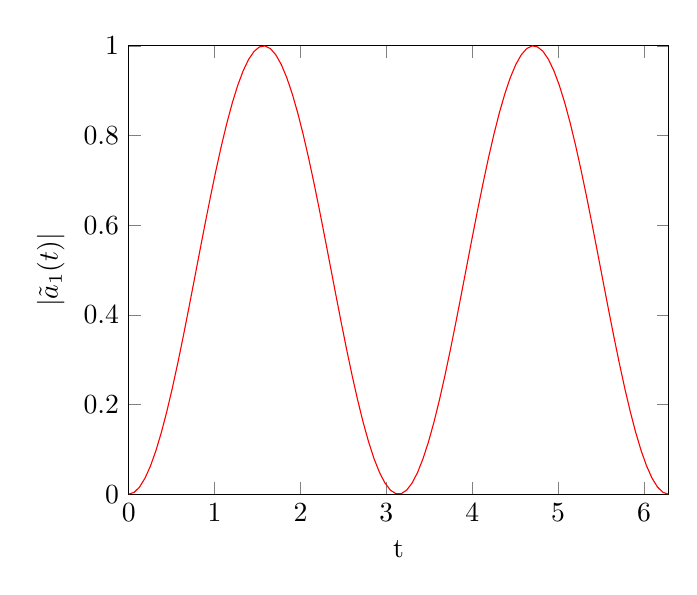
\begin{tikzpicture}
	\begin{axis}[
	    ylabel={$\left|\tilde{a}_1(t)\right|$},
	    xlabel=t,
	    xmin= 0, xmax= 2*pi,
	    ymin= 0, ymax =1,
	]
	\addplot[domain=0:2*pi, samples=100,color=red]{sin(deg(x))^2};
	\end{axis}
    \end{tikzpicture}
    \caption{$\left|\tilde{a}_1(t) \right|$ }
    \label{ddd}
\end{figure}
Il periodo di queste oscillazioni è $2\pi /\Omega_r$ , al tempo $\pi /\Omega_r = T_\pi$ il sistema si è "ribaltato": ha probabilità massima 1 di essere nel primo eccitato.
\begin{figure}[H]
    \centering
    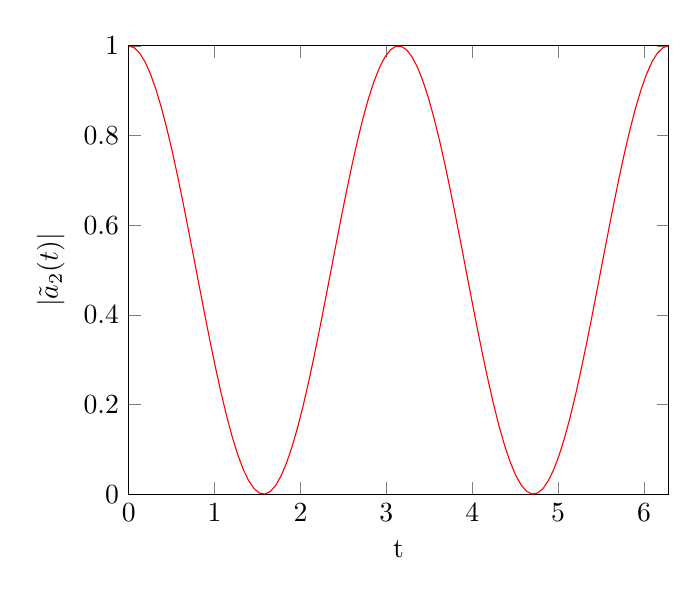
\begin{tikzpicture}
	\begin{axis}[
	    ylabel={$\left|\tilde{a}_2(t)\right|$},
	    xlabel=t,
	    xmin= 0, xmax= 2*pi,
	    ymin= 0, ymax =1,
	]
	\addplot[domain=0:2*pi, samples=100,color=red]{cos(deg(x))^2};
	\end{axis}
    \end{tikzpicture}
    \caption{$\left|\tilde{a}_2(t) \right|$.}
    \label{1111}
\end{figure}
Possiamo spiegarci questa cosa pensandola come tanti processi perturbativi consecutivi: il nostro atomo parte nel fondamentale ed interagendo con la radiazione passa nel primo eccitato. 
Arrivato nel livello eccitato non può più assorbire radiazione, può solo fare emissione stimolata ricadendo nel fondamentale.\\
Notiamo che la probabilità di transizione non è lineare nel tempo (come potevamo aspettarci per $\tau$ molto piccoli), inoltre tale soluzione deve contenere il trattamento perturbativo, quindi per tempi piccoli (ovvero tali da far rimanere la probabilità di transizione piccola). \\
Questo ci dice anche che l'approccio perturbativo vale per 
\[
\tau \ll \frac{2\pi}{\Omega_r}
.\] 
Possiamo anche risolvere le equazioni nel caso di $\delta \neq 0$, si ottiene:
\[
\left|\tilde{a}_1\right|^2= \frac{\Omega^2_r}{\Omega_r^2+\delta^2}
\sin^2\left(\frac{\sqrt{\Omega^2_r + \delta^2}}{2}t\right)
.\] 
Quindi la forma di $\left|\tilde{a}_1\right|^2$ si modifica nel seguente modo:
\begin{figure}[H]
    \centering
    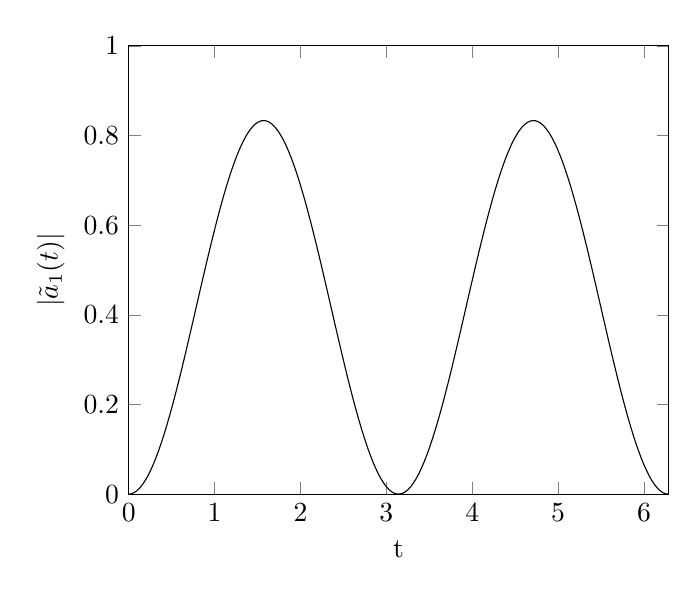
\begin{tikzpicture}
	\begin{axis}[
	    ylabel={$\left|\tilde{a}_1(t)\right|$},
	    xlabel=t,
	    xmin= 0, xmax= 2*pi,
	    ymin= 0, ymax = 1,
	]
	\addplot[domain=0:2*pi, samples=200]{5/6*sin(deg(x))^2};
	\end{axis}
    \end{tikzpicture}
    \caption{$\left|\tilde{a}_1(t)\right|$ considerando $\delta\neq 0$.}
    \label{delta non nullo}
\end{figure}
Con questa ultima equazione capiamo che l'approssimazione RWA è sensata, la correzione a questa sarebbero delle oscillazioni molto piccole sovrapposte all'andamento già oscillante. \\
Per poter visualizzare le onde di Rabi è necessario avere delle onde quanto più possibile monocromatiche, altrimenti la convoluzione di tutte le componenti oscillanti distruggerà la forma della oscillazione. \\
Per poter vedere tali oscillazioni quindi sarà necessario avere una ampiezza della distribuzione in frequenza $\Delta\omega$ pari a:
\[
\Delta\omega\ll\Omega_r
.\] 
Quindi gli esperimenti in questo campo si fanno tipicamente con Laser molto intensi.
\subsection{Interazione radiazione materia collegata alla termodinamica}%
\label{sub:Interazione radiazione materia collegata alla termodinamica}
Supponiamo di avere una Ensemble di N atomi, la probabilità al tempo $t$  di avere l'atomo nel livello $m$-esimo è $\left|a_m(t) \right|^2$. Il numero di atomi nel livello $m$-esimo al tempo $t$  sarà dato da:
\[
    N_m = N\left|a_m(t) \right|^2
.\] 
La probabilità di transizione l'abbiamo calcolata e supponiamo che gli atomi non abbiano altri tipi di interazione al di fuori del campo elettromagnetico. Possiamo quindi scrivere che:
\[
    \frac{\text{d} \left|a_n(t) \right|^2_\text{in} }{\text{d} t} =
    P_{m\to n}\left|a_m(t) \right|^2
.\] 
Viceversa:
\[
    \frac{\text{d} \left|a_m(t) \right|^2_\text{in} }{\text{d} t} =
    P_{n\to m}\left|a_n(t) \right|^2
.\] 
Questa è la probabilità che l'atomo vada nel livello $n$  per la prima formula e $m$  per la seconda.\\
La probabilità di uscire dal livello $n$  sarà invece:
\[
    \frac{\text{d} \left|a_n(t)\right|^2_\text{out} }{\text{d} t} =
    -\frac{\text{d} \left|a_n(t) \right|^2_\text{in} }{\text{d} t}=
    -P_{n\to m}\left|a_n\right|^2
.\] 
In totale (per tutti gli atomi) si ha che:
\[
\frac{\text{d} N_n}{\text{d} t} = \sum_{m}^{'} P_{m\to n}N_m 
-\sum_{m}^{'} P_{n\to m}N_n
.\] 
Le sommatoria sono su tutti i livelli diversi da $n$, la prima corrisponde al prodotto della probabilità di andare da $m$  a $n$  moltiplicata per gli atomi del livello $m$  (e poi sommiamo su tutti gli $m\neq n$) mentre il secondo termine corrisponde agli atomi che abbandonano il livello $n$.\\
Se siamo all'equilibrio ovviamente tale derivata deve essere nulla:
\[
\sum_{m}^{'} P_{m\to n}N_m =
\sum_{m}^{'} P_{n\to m}N_{n}
.\] 
Notiamo che stiamo ragionando sui moduli quadri delle ampiezze di probabilità, quindi quando facciamo una trattazione di rate abbiamo già perso un po di informazione (nella trattazione di Rabi invece potevamo vedere anche le fasi della ampiezza di probabilità), per questo motivo non siamo in grado di descrivere fenomeni coerenti o interferenze.\\
L'equazione per l'equilibrio che abbiamo trovato è parente di un'altra ancora più stringente che abbiamo già incontrato: l'equazione di bilancio dettagliato.\\
Infatti il bilancio dettagliato ci diceva che i singoli processi dai singoli stati devono essere uguali:
\[
\forall n,m \quad P_{m\to n}N_m = P_{n\to m}N_n 
.\] 
Dal punto di vista quantistico questa è strettamente connessa con il time revelsal simmetry.\\
Dal punto di vista classico (sistema alla Boltzmann) se prendiamo un sistema a due livelli sappiamo che all'equilibrio termico:
\[
    \frac{N_1^0}{N_2^0}= \frac{g_1}{g_2}\exp\left(-\frac{E_{12}}{kT}\right)
.\] 
Se gli atomi possono interagire solo con il campo elettromagnetico allora si ha che:
\[
P_{12} = B_{12}u_{\nu_{12}}=P_{21}=B_{21}u_{\nu_2}
.\] 
Applicando il bilancio dettagliato abbiamo che:
\[
\frac{N_1^0}{N_2^0} = \frac{P_{2\to 1}}{P_{1\to 2}} = 1
.\] 
Quindi sembra che le condizioni di equilibrio termodinamico e la condizione di equilibrio proveniente da un principio generale applicato all'interazione con il campo EM ci diano risultati diversi. \\
Einstein risolse questo problema assumendo che le probabilità fossero proporzionali alla intensità del campo elettromagnetico, egli introdusse un nuovo processo di emissione scrivendo:
\[
    P_{1\to 2}= B_{1\to 2}u_{\nu}(\nu_{12})  + A_{1\to 2}
.\] 
Il secondo termine è indipendente dalla densità di energia del campo elettromagnetico. Questo coefficiente è quello di emissione spontanea \footnote{Quantizzando il campo EM si vedrà che tale elemento viene fuori direttamente dagli elementi di matrice della interazione.}.\\
Possiamo ora scrivere le proprietà di equilibrio termodinamico:
\[
    \frac{N_1^0}{N_2^0} = \frac{B_{1\to 2 u_\nu(\nu_{12})}}{B_{1\to 2}u_\nu(\nu_{12}) + A_{1\to 2}} = \frac{g_1}{g_2}e^{-h\nu_{12} /k_BT}
.\] 
Possiamo quindi calcolare $A$  in funzione di $T$  :
\[
    A_{12} = \left(B_{1\to 2}\frac{g_2}{g_1}e^{h\nu_{12} /k_BT}-B_{1\to 2}\right)u_\nu(\nu_{12}) 
.\] 
Se siamo all'equilibrio termico possiamo utilizzare l'espressione di plank:
\[
A_{1\to 2} =
\frac{8\pi h\nu_{12}^3}{c^3}\left(\frac{B_{2\to 1}\frac{g_2}{g_1}e^{h\nu_{12} /k_BT}-B_{1\to 2}}{e^{h\nu_{12} /k_BT}-1}\right)
.\] 
Imponendo che tale coefficiente non dipenda dalla temperatura abbiamo che $B_{1\to 2}g_1=B_{2\to 1}g_2$, quindi rimane semplicemente:
\[
A_{1\to 2}=\frac{4}{3\hbar }\frac{\omega_{12}^3}{c ^3}\left|\bra{1}d\ket{2}\right|^2
.\] 
Questa è l'espressione del coefficiente di emissione spontanea, quella che si ottiene anche quantizzando il campo elettromagnetico.\\
Vediamo che dipende dal cubo della frequenza e dal modulo quadro del dipolo. Se siamo in una situazione di assenza del campo EM rimane l'emissione spontanea e troviamo dalla equazione di rate semplicemente un decadimento esponenziale con tempo caratteristico:
\[
\tau_{s}=\frac{1}{A_{1\to 2}}
.\] 
Diamo una dimensione numerica del tempo tipico di emissione spontanea:
\[
    \left|\bra{1}d\ket{2}\right|\approx ea \approx 2.4 \text{ Debye} = 2.4\cdot 10^{-30}\text{ [C][m]}
.\] 
Nel visibile ($\lambda\sim 600$ nm) abbiamo che il tempo di emissione spontanea viene $\tau_s \sim 100$  ns.\\
Se andiamo nell'infrarosso ($\lambda  = 10$ $\mu$m) abbiamo $\tau_s\sim 0.5$  ms.\\
Nel caso quantistico la trattazione fatta resta valida, tuttavia se cambiamo il tipo di particella sarà necessario cambiare l'assunzione che 
\[
\frac{\text{d} N_1}{\text{d} t} \propto N_{2}P_{21}
.\]   
Con particelle classiche questo funziona, con con particelle quantistiche invece no. \\
Prendiamo come esempio il caso di Fermioni: il rate con cui le particelle vanno dallo stato 1 a quello 2 deve tener conto del fatto che non ci può stare più di una particella per stato, gli stati finali devono essere liberi per transire.\\
Nel caso di Bosoni invece si ha che più particelle ci sono nello stato finale e più e probabile che un'altra particella ci finisca.\\
Vediamo adesso quando domina il processo di emissione stimolata e quando invece domina quello di emissione spontanea. Per far questo consideriamo il rapporto:
\[
    \frac{B_{1\to 2}u_\nu(\nu_{12})}{A_{1\to 2}} = \frac{1}{e^{h\nu_{12} /kT}-1}
    = n_\text{ph}^{(\nu_{12})} = n_{\nu_{12}}
.\] 
Questo è il numero medio di fotoni alla frequenza $\nu_{12}$  che è la frequenza della transizione. Quantizzando il campo magnetico troviamo che $P_\text{em} \propto n_\text{pH} + 1$, il primo termine sarà quello si emissione stimolata mentre quello di emissione spontanea è il secondo.\\
Questo comporta che in una situazione in cui $n_{\nu_{12}}\ll 1$ allora domina l'emissione spontanea, viceversa domina la stimolata.\\
Nel primo dei due casi se abbiamo fotoni termici la condizione comporta:
\[
e^{h\nu /kT}\ll 2
.\] 
Di conseguenza anche:
\[
    T\lambda\gg \frac{1}{\ln(2)}\frac{hc}{k}\sim 20000 [\mu\text{m}][\text{K}]
.\] 
L'emissione stimolata domina quindi per $\lambda\gg 10^4$.\\
\subsection{Applicazione dell'interazione radiazione materia: Laser}%
\label{sub:Applicazione dell'interazione radiazione materia: Laser}
Vediamo come varia l'intensità della radiazione quando attraversa un mezzo materiale (che noi schematizziamo come un sistema a due livelli). Dobbiamo studiare la variazione della intensità $I$  della radiazione (il flusso di energia per unità di tempo, la potenza per unità di area), ricordando che
\[
u = \frac{E_0^2}{8\pi}
.\] 
Questa è la densità di energia (nel corpo nero avevamo $u_\nu$: la densità di energia per unità di frequenza). Abbiamo quindi
\[
I=cu
.\] 
Considerando il seguente corpo
\begin{figure}[ht]
    \centering
    \incfig{corpo-per-interazione-radiazione-materia}
    \caption{Corpo per interazione radiazione materia}
    \label{fig:corpo-per-interazione-radiazione-materia}
\end{figure}
Vogliamo trovare l'andamento di $I_z$, in particolare vedremo che
\[
    I=\exp\left(-kz\right)I(0) 
.\] 
O in forma differenziale:
\[
    dI = -k I(z)dz
.\] 
Dove il segno negativo è per la convenzione che una variazione di intensità negativa si riferisce ad un $k$  positivo.\\
In generale $k$  potrebbe dipendere da $I$, al primo ordine non sarà così, $k$  si dice coefficiente di assorbimento.
Se tale parametro è positivo l'energia viene soppressa, se è negativo l'energia aumenta.\\
Per un sistema a due livelli questo significa che se $k$  è positivo l'energia viene persa dal campo elettromagnetico perché domina l'assorbimento, viceversa domina l'emissione stimolata.\\
Poniamoci nella situazione in cui $N_2$  ed $N_1$  (le popolazioni dei due livelli) sono fissate e diventano da qui in poi le densità di popolazione \footnote{Facciamo in modo che non si modifichino con l'applicazione di un campo elettromagnetico esterno}.
Consideriamo la variazione di $I$  in $z$  :
\[
\frac{\text{d} I}{\text{d} z} = c \frac{\text{d} u}{\text{d} z} 
= \frac{\text{d} z}{\text{d} t} \frac{\text{d} u}{\text{d} z} = \frac{\text{d} u}{\text{d} t} 
.\]
Ma l'ultima derivata la possiamo scrivere considerando che la densità di energia del campo EM cambia tramite processi di assorbimento o di emissione stimolata, trascuriamo l'emissione spontanea poiché consideriamo un campo elettromagnetico che si propaga con un vettore d'onda fissato nel nostro materiale. \\
Non abbiamo parlato le proprietà dei fotoni emessi nei vari processi, tuttavia i fotoni emessi per emissioni stimolata sono identici ai fotoni che li hanno stimolati, quelli emessi per emissione spontanea invece possono essere emessi in uno qualunque dei modi possibili del campo elettromagnetico, in particolare con un qualunque $k$. Per questo motivo li trascuriamo.\\
Abbiamo quindi processi di assorbimento o processi di emissione stimolata, per unità di tempo si produrranno tanti fotoni quanti atomi passano dal livello eccitato al fondamentale (per unità di tempo) e viceversa.
\[
\frac{\text{d} n^+}{\text{d} t} = \left|\frac{\text{d} N_1}{\text{d} t} \right|_\text{out} 
= P_{1\to 2}N_1
.\] 
\[
\frac{\text{d} n^-}{\text{d} t} =\left|\frac{\text{d} N_1}{\text{d} t} \right|_\text{out} = P_{2\to 1}N_2
.\] 
Quindi abbiamo che 
\[
\frac{\text{d} I}{\text{d} z} = \frac{\text{d} u}{\text{d} t} =
h\nu \left(P_{1\to 2}N_1 - P_{2\to 1}N_2\right)
.\] 
Inserendo dentro $P_{1\to 2}$  e $P_{2\to 1}$:
\[
    P_{1 \to 2} = B_{12}u_\nu (\nu_{12}) 
.\] 
Questa volta supponiamo che la radiazione sia molto "stretta" rispetto alla $g$, integriamo la $u_\nu$  lasciando la $g$.  \\
\[
    P_{1 \to 2} = B_{12}g(\nu-\nu_{12})u
.\] 
Inserendo dentro otteniamo l'espressione:
\[
    \frac{\text{d} I}{\text{d} z} = h\nu g(\nu-\nu_{12}) u\left(B_{1\to 2}N_1
    -B_{2\to 1}N_2\right)= -kI
.\] 
Nella formula abbiamo riscritto $u = I /c$  mentre il coefficiente $k$  vale:
\[
    k=\frac{h\nu}{c}g(\nu-\nu_{12})\left(B_{21}N_2 - B_{12}N_1\right) 
.\] 
All'equilibrio termodinamico la popolazione del livello i-esimo la popolazione sarà moltiplicata per la degenerazione del livello:
\[
N_i^0 = \frac{g_i e^{- E_i /kT}}{Z}
.\] 
Quindi abbiamo che:
\[
\frac{N_1^0}{N_2^0} = \frac{g_1}{g_2}e^{-E_{12} /kT}
.\] 
Inoltre
\[
\frac{B_{21}}{B_{12}} = \frac{g_1}{g_2}
.\] 
Anche con la degenerazione invece $A$ resta lo stesso. Supponiamo adesso che le degenerazioni siano uguali, il coefficiente di assorbimento diventa
\[
    k=\frac{h\nu}{c}g(\nu-\nu_{12}) (N_2-N_1) 
.\] 
Quindi il coefficiente di assorbimento è positivo quando $N_2$ è maggiore di $N_1$. \\
Se si riesce ad invertire la popolazione (cioè ad avere $N_1>N_2$) allora il coefficiente $k$ diventa negativo e la radiazione aumenta esponenzialmente nel passaggio nel materiale. 

\lez{26}{23-04-2020}{}
Abbiamo assunto nella trattazione che le popolazioni dei livelli $\ket{1}$ e $\ket{2}$ rimanessero invariate incidendo con della radiazione sul sistema, in generale questa assunzione non è rispettata.\\ 
Può infatti capitare di avere un oggetto completamente passivo che viene fatto attraversare dalla radiazione, ci aspettiamo che aumentando l'intensità della radiazione il numero di atomi eccitati da quest'ultima cresca: 
\[
    I\nearrow\implies N_1\nearrow
.\] 
Più atomi si eccitano e meno probabilità avremo di fare assorbimento.
Ci saranno poi dei processi che tengono a riportare il sistema in una condizione di equilibrio termodinamico (emissione spontanea, collisioni con i fononi o con le pareti del contenitore).\\
Cerchiamo di modellizzare questo sistema, vedremo che il coefficiente di assorbimento in questo caso dipenderà dalla intensità.\\
Il coefficiente trovato nella scorsa lezione è:
\[
    k = \frac{h\nu}{c}g(\nu-\nu_{12}) \left(N_2-N_1\right)
.\] 
Dove $g(\nu-\nu_{12})$ è la forma di riga della transizione. Ricordiamo anche che il livello superiore è (1) mentre il livello inferiore è il (2) e che le popolazioni sono definite per unità di volume.
Oppure se la degenerazione dei livelli è diversa abbiamo:
\[
    k = \frac{h\nu}{c}g(\nu-\nu_{12}) \left(B_{21}N_2-B_{12}N_1\right)
.\] 
Descriviamo un sistema che abbia popolazione dei livelli variabile:
\[\begin{aligned}
    \frac{\text{d} N_1}{\text{d} t} =& B_{21}N_2g(\nu-\nu_{12}) u 
    -B_{12}N_1 u g(\nu-\nu_{12}) =\\
	&=\left(B_{21}N_2- B_{12}N_1\right)ug(\nu-\nu_{12}) 
.\end{aligned}\]
Ovviamente per l'altro livello abbiamo la stessa cosa con il segno opposto:
\[
    \frac{\text{d} N_2}{\text{d} t} = -\frac{\text{d} N_1}{\text{d} t}
.\] 
La differenza delle ultime due equazioni ci da:
\[
    \frac{\text{d} \left(N_2-N_1\right)}{\text{d} t} =
    2\left|B_{21}N_1-B_{21}N_2\right|u g(\nu-\nu_{12}) 
.\] 
Questa riguarda l'interazione con il campo elettromagnetico, dobbiamo tener di conto anche dei processi che riportano il sistema all'equilibrio: introduciamo quindi il parametro $\gamma_{\parallel}$.
\begin{defn}[Rate di ritorno all'equilibrio]{defn:Rate di ritorno all'equilibrio}
Definiamo il rate di ritorno all'equilibrio come $\gamma_\parallel$, questo termine è un termine Euristico che ci descrive il ritorno all'equilibrio nella equazione per $N_2-N_1$. 
\end{defn}
Descriviamo la configurazione di equilibrio con le popolazioni $N_1^0$ e $N_2^0$ che seguono la distribuzione di Boltzmann:
\[
    \frac{N_2^0}{N_1^0} = \frac{g_2}{g_1}e^{-\left(E_2-E_1\right) /kT}
.\] 
Supponendo che questo nuovo rate descriva dei processi che tendono a far tornare il sistema all'equilibrio in modo esponenziale aggiungiamo un termine alla equazione del trasporto (come abbiamo fatto per l'equazione del trasporto) del tipo:
\[
    \frac{\text{d} \left(N_2-N_1\right)}{\text{d} t} =
    -2\left|B_{21}N_2-B_{12}N_2\right|u g(\nu-\nu_{12}) 
    +\gamma_{\parallel}\left[\left(N_2^0-N_1^0\right)-
    \left(N_2-N_1\right)\right]
.\] 
Il termine aggiunto è un termine lineare in tale equazione che tiene di conto della differenza tra la situazione di equilibrio e quella fuori equilibrio che consideriamo.\\
Possiamo quindi riscrivere l'equazione di Rate assumendo anche $B_{12}=B_{21}$:
\[
    \frac{\text{d} \left(N_2-N_1\right)}{\text{d} t} =
    \gamma_{\parallel}\left[N_2^0-N_1^0 - \left(N_2-N_1\right)\right]
    -2g(\nu-\nu_{12}) \frac{I}{c}B_{21}\left(N_2-N_1\right)
.\] 
Introducendo questo parametro di rate adesso possiamo di nuovo assumere che la derivata sia nulla (soluzioni stazionarie) quindi possiamo ricavare che:
\[
    N_2-N_1 = \frac{N_2^0-N_1^0}{1+2g(\nu-\nu_{12})
    \frac{B}{\gamma_{\parallel}c}I}=
    \frac{N_2^0-N_1^0}{1+\frac{I}{I_s(\nu)}}
.\] 
In cui per compattare l'espressione si introduce:
\begin{defn}[Intensità di dimezzamento]{defn:Intensità di dimezzamento}
L'intensità per la quale la differenza delle popolazioni si dimezza rispetto al valore di equilibrio è:
\[
    I_s = \frac{\gamma_\parallel c}{2B_{21}g(\nu-\nu_{12})}
.\] 
\end{defn}
All'aumentare dell'intensità la differenza di popolazioni tra il fondamentale ed il livello di sopra diventa più piccolo, questo perché a stazionarietà ho sempre più processi che tengono ad eccitare gli atomi quindi il $\gamma_\parallel$  non riesce a riportare il sistema esattamente all'equilibrio. \\
Se l'intensità tende a $\infty$ allora i due livelli tendono ad avere la stessa popolazione ($N_2-N_1\to 0$)
\footnote{Questo indipendentemente dalle dimensioni di $\gamma_\parallel$.}.
\begin{fact}[Con due livelli niente inversione]{fact:Con due livelli niente inversione}
Per un sistema a due livelli a stazionarietà non è possibile fare inversione di popolazione inviando una radiazione elettromagnetica, al massimo si riesce a fare $N_2=N_1$.
\end{fact}
Dobbiamo notare che questo approccio non contraddice le oscillazioni di Rabi, in questo caso siamo a stazionarietà mentre con tali oscillazioni non siamo stazionari. \\
Possiamo riscrivere il coefficiente di assorbimento inserendo il nuovo valore di $N_2-N_1$:
\[
    k= \frac{h\nu}{c}g(\nu-\nu_{12})B_{21} \frac{N_2^0-N_1^0}{1+\frac{I}{I_s}}=
    \frac{k_0}{1+\frac{I}{I_S}}
.\]
\begin{figure}[H]
    \centering
    \begin{tikzpicture}
	\begin{axis}[
	    xmin= 0, xmax= 11,
	    ymin= 0, ymax = 11,
	    xlabel={$I$},
	    ylabel={$k$},
	    axis lines = middle,
	    ytick={10},
	    yticklabel={$k_0$},
	    xtick={0}
	]
	\addplot[domain=0:10, samples=100]{10*1/(1+x)};
	\end{axis}
    \end{tikzpicture}
    \caption{Andamento di $k$ al variare della intensità.}
    \label{Andamento di k0 al variare della intensità.}
\end{figure}
\noindent
Questo fenomeno si chiama saturazione: aumentando l'intensità esauriscono gli atomi nel fondamentale. L'equazione di propagazione risulta quindi adesso modificata, la soluzione non ci porta più ad un esponenziale:
\[
    \text{d}I=-\frac{k_0}{1+\frac{I}{I_s}}I \text{d}z
.\] 
Il coefficiente di assorbimento è molto utilizzato da chi studia solidi, chi invece studia atomi o impurezze usa la sezione d'urto. Quest'ultima è in relazione al coefficiente di assorbimento tramite la seguente:
\[
    k = \sigma\left(\frac{B_{21}}{B_{12}}N_2-N_1\right)
.\] 
Possiamo anche riscrivere la $\sigma_0$:
\[
    \sigma_0=\frac{h\nu}{c}Bg(\nu-\nu_{12}) =
    \left[\frac{\lambda_{12}}{2}\right]^2Ag(\nu-\nu_{12}) 
.\] 
Dove $\lambda_{12}$ è la lunghezza d'onda della transizione: 
\[
    \lambda_{12} = \frac{c}{\nu_{12}}
.\] 
Siamo interessati a sistemi in cui $N_1>N_2$ in modo tale che il nostro mezzo sia in grado di amplificare la radiazione (coefficiente di assorbimento negativo). Possiamo far questo senza usare una eccitazione ottica (utilizzando ad esempio una eccitazione elettrica con il trasporto di carica).\\
Tuttavia l'inversione di popolazione storicamente si ottiene tramite sistemi ottici, il modo più semplice per farcela è con un sistema a tre livelli. Tipicamente i sistemi a tre livelli descrivono bene i Maser (Laser per le Microonde) che sono venuti prima dei sistemi ottici.
\subsection{Inversione di popolazione per un sistema a 3 livelli}%
Prendiamo un sistema a 3 livelli
\begin{figure}[ht]
    \centering
    \incfig{sistema-a-3-livelli}
    \caption{Sistema a 3 livelli}
    \label{fig:sistema-a-3-livelli}
\end{figure}
Supponiamo di essere nelle microonde e di avere tutte e due le differenze di energia minori di $kT$:
\[\begin{aligned}
    &h\nu_{12}\ll kT\\
    &h\nu_{23}\ll kT
.\end{aligned}\] 
Andiamo a pompare dall'esterno tra i livelli (3) e (1), in questo modo se la pompa è molto intensa le popolazioni in $\ket{1}$ e $\ket{3}$ possono diventare circa uguali:
\[
    N_1\approx N_3
.\] 
Supponiamo che la popolazione del livello (2) sia legata agli altri due semplicemente dall'equilibrio termodinamico 
\footnote{(2) si accorge della popolazione di (1) e (3) per via dei processi di rilassamento che tendono a riportare il sistema in equilibrio.}.
Possiamo quindi dire che (sviluppando al primo ordine gli esponenziali con $h\nu\ll kT$) :
\[\begin{aligned}
    &N_3^0 
    \approx N_2^0\left(1+ \frac{h\nu_{23}}{kT}\right)\\
    &N_1^0 
    \approx N_2^0\left(1-\frac{h\nu_{12}}{kT}\right)
.\end{aligned}\]
Dove i segni diversi sono dovuti al fatto che nel primo caso i pedici sono stati invertiti.\\
Nella ipotesi in cui $N_1\sim N_3$ possiamo fare una media:
\[
    N_1\sim N_3 = N_2^0\left(1+ h \frac{\nu_{23}-\nu_{12}}{2kT}\right)
.\] 
Se siamo nella ipotesi in cui $\nu_{23}>\nu_{12}$ allora abbiamo che $N_1>N_2$ e si ha inversione di popolazione nel seguente punto:
\begin{figure}[H]
    \centering
    \incfig{inversione-di-popolazione-1-2}
    \caption{Inversione di popolazione 1-2}
    \label{fig:inversione-di-popolazione-1-2}
\end{figure}
\noindent
viceversa se $\nu_{23}<\nu_{12}$ abbiamo che $N_2<N_3$, quindi:
\begin{figure}[H]
    \centering
    \incfig{inversione-di-popolazione-2-3}
    \caption{Inversione di popolazione 2-3}
    \label{fig:inversione-di-popolazione-2-3}
\end{figure}
\noindent
Quindi pompando i livelli (1) e (3) possiamo invertire la popolazione di altri due livelli. 
Con questa ulteriore inversione abbiamo che $k<0$, quindi nel propagarsi della radiazione nel nostro mezzo essa cresce esponenzialmente (almeno fino a che la popolazione non satura nel nuovo livello).
\subsection{Laser}%
Un sistema che inverte la popolazione è alla base della amplificazione della radiazione. Se aggiungiamo a quest'ultimo un oscillatore con feedback possiamo avere un dispositivo auto-oscillante dal momento che il guadagno diventa maggiore od uguale delle perdite.\\
Utilizzando degli specchi è quindi possibile, sfruttando l'inversione di popolazione, creare un sistema auto-oscillante molto selettivo in frequenza: un laser
\footnote{Light Amplification by Stimulated Emission of Radiation} 
(o maser nelle micro-onde). \\ 
Notiamo che si chiama Laser nonostante questo sia solo un oscillatore, non un amplificatore. L'amplificatore è un oggetto identico al laser ma senza gli specchi
\footnote{Il nome corretto sarebbe stato Loser, non era tuttavia un nome carino da dare ad una tecnologia tanto preziosa\ldots}.
Un laser per poter auto-oscillare deve avere un mezzo che guadagna (che abbiamo descritto) e dobbiamo inserire un circuito di Feedback (la cavità).\\
Un esempio di cavità può essere un sistema di 4 specchi
\begin{figure}[H]
    \centering
    \incfig{sistema-di-specchi-per-il-laser}
    \caption{Sistema di specchi per il Laser}
    \label{fig:sistema-di-specchi-per-il-laser}
\end{figure}
\noindent
Uno di questi specchi dovrebbe essere semitrasparente se vogliamo che esca qualcosa da questo dispositivo. Notiamo che è la cavità che determina la frequenza di emissione.\\
C'è poi un ulteriore tipo di cavità ottica che sfrutta soltanto 2 specchi facendo passare la radiazione 2 volte per periodo nell'amplificatore, concentriamoci su questo tipo di cavità.\\
Supponiamo che la cavità abbia volume $V$ (con gli specchi di superficie $S$ ed una distanza $L$ tra questi)  e che all'interno la densità di energia del campo EM sia uniforme, in questo modo l'energia totale all'interno della cavità sarà
\[
W = V\cdot u = S\cdot L\cdot u
.\] 
Questa cavità avrà delle perdite, la potenza persa dalla cavità sarà
\[
P_d+P_u
.\] 
In cui $P_d$  è quella dissipata da aria, dagli specchi imperfetti ecc\ldots mentre $P_u$  è la potenza persa a causa dello specchio semitrasparente, quest'ultima è quella che vogliamo: quella che ci dà la luce.\\
Possiamo inglobare queste informazioni introducendo un tempo medio in cui la radiazione esce dalla cavità $\tau$:
\[
\frac{\text{d} W}{\text{d} t} = - \frac{W}{\tau}
.\] 
Dove possiamo immaginare $\tau$ come il tempo di vita media dei fotoni nella cavità.\\
Assumiamo quindi fenomenologicamente che l'energia nella cavità venga persa in modo esponenziale. Solitamente anziché usare $\tau$  si usa il fattore di qualità della cavità:
\[
Q = \omega\tau
.\] 
Nella quale $\omega$ è la frequenza di risonanza determinata dalla fase (per avere un sistema auto-oscillante bisogna che dopo un giro nella cavità ottica il campo sia in fase per avere interferenza costruttiva).\\
Quindi l'uguaglianza "Guadagno = Perdite" ci dirà la condizione di soglia per la quale il sistema è in grado di auto-oscillare, la frequenza di oscillazione sarà fissata dalla fase che a sua volta sarà determinata dalla lunghezza della cavità.\\
Ribadiamo che $\omega$ è data dai modi risonanti del campo elettromagnetico che esistono nella cavità permessi dalle condizioni al contorno (dipendenti dalla lunghezza).
\subsubsection{Distribuzione Lorentziana della densità di energia uscente dal Laser}%
Supponiamo che all'interno della cavità il campo EM sia uniforme:
\[
    E(t) = E(0) \exp\left(-i\omega t- \frac{t}{2\tau}\right)
.\] 
Dove abbiamo inserito un fattore $1 /2$ perché $\tau$ è definito sull'energia che va come il quadrato del campo.\\
A noi interessa la coerenza di questa radiazione, per vederla possiamo effettuare una trasformata di Fourier:
\[\begin{aligned}
    E(\Omega) =& \frac{1}{\sqrt{2\pi} }\int_{0}^{\infty} E(t) e^{i\Omega t}dt=\\
    =&
    \frac{1}{\sqrt{2\pi}}E(0)\int_{0}^{\infty} 
    \exp\left(i\left[\left(\Omega -\omega\right)+ \frac{i}{2\tau}\right]t\right) dt=\\
    =&
    \frac{1}{\sqrt{2\pi}}
    \frac{E(0)}{i\left[\left(\Omega-\omega\right)+\frac{i}{2\tau}\right]}
.\end{aligned}\]
Quindi se prendiamo la $u(\Omega)$:
\[
    u(\Omega) = \frac{\left|E(\Omega)\right|^2}{8\pi} = \frac{1}{16\pi} 
    \frac{\left|E(0)\right|^2}{\left(\Omega-\omega\right)^2+ \frac{1}{4\tau^2}}
.\] 
\begin{figure}[H]
    \centering
    \begin{tikzpicture}
	\begin{axis}[
	    xmin= 0, xmax= 13,
	    ymin= 0, ymax = 10,
	    axis lines = middle,
	    xlabel={$\Omega$},
	    ylabel={$u(\Omega)$},
	    xtick={0,5},
	    ytick={0},
	    xticklabel={$\omega$},
	    %yticklabel={$$},
	]
	\addplot[domain=0+9/10*0:10+9/10*10, samples=100]{1/((x-5)^2+1/9)};
	\addplot +[mark=none,black,dotted] coordinates {(5, 0) (5, 9)};
	\end{axis}
    \end{tikzpicture}
    \caption{Distribuzione in frequenza di $u(\Omega)$.}
    \label{Lorentziana}
\end{figure}
\noindent
Avere un tempo $\tau$ di decadimento dei fotoni dalla cavità si traduce in una distribuzione Lorentziana piccata attorno ai modi risonanti $\omega$ e larga
\[
  \Delta\omega_c = \frac{1}{\tau}=\frac{\omega}{Q}  
.\] 
Di conseguenza possiamo scrivere anche che il fattore di qualità è:
\[
Q = \frac{\omega}{\Delta\omega}
.\] 
Quindi migliori sono gli specchi e più la distribuzione tende ad una $\delta$.
\subsubsection{Esempio: perdite dovute solo alle riflessioni sugli specchi}%
Se ci fossero solo le perdite per riflessione descritte da un coefficiente $R$ (detto riflettività: la capacità di riflettere dello specchio) possiamo chiederci come andrebbe il fattore di qualità. Ipotizziamo di avere uno specchio di area $S$ in una cavità lunga $L$, l'energia che incide per unità di tempo sullo specchio (Potenza incidente) è:
\[
E_\text{specchio} = \frac{Su\text{d}z}{\text{d}t} = Suc
.\] 
L'energia che viene trasmessa dagli specchi dalla riflessione è:
\[
E_\text{Lost} = SucR
.\] 
Quindi il fattore di qualità è:
\[\begin{aligned}
    Q &= \omega\tau = \\
      &= \omega  \frac{W}{P_u} =\\
      &=\omega\frac{SLu}{\left(1-R\right)Scu} =\\
      &=2\pi \frac{L}{\lambda } \frac{1}{1-R}
.\end{aligned}\]
La potenza in uscita dall'oggetto è data da quella incidente meno quella trasmessa dagli specchi (che non esce poiché riflessa) : $W = \left(1-R\right)Scu$.\\
Otteniamo allora i limiti asintodici:
\begin{itemize}
    \item Laser Buono: $R\to 1 \implies  Q\to \infty \implies  \Delta\omega\to 0$, nessuna perdita.
    \item Laser pessimo: $R\to 0 \implies  2\pi  L /\lambda$.
\end{itemize}
Notiamo che in generale il fattore $Q$ è direttamente proporzionale a $L$, quindi una cavità più grande crea una radiazione più coerente.\\
Possiamo capire quest'ultima osservazione considerando che più è lunga la cavità e meno volte la radiazione va a sbattere nello specchio, se la radiazione rimbalza meno volte le perdite saranno minori.\\
Facciamo un esempio numerico:
\begin{itemize}
    \item $L=50$ cm.
    \item $\lambda = 500$nm.
    \item $R = 0.98$. 
\end{itemize}
Con questi valori riusciamo ad ottenere $Q = 3\cdot 10^8$.\\
\subsection{Condizioni di auto-oscillazione per un sistema}%
Vediamo adesso di risolvere il seguente problema, esposto da due punti di vista diversi:
\begin{enumerate}
    \item Data l'inversione di popolazione troviamo $Q$ affinché il sistema oscilli.
    \item Dato $Q$ troviamo l'inversione di popolazione per avere un sistema auto-oscillante.	
\end{enumerate}
Normalmente il modo giusto di porsi la domanda è il secondo, infatti possiamo cambiare $N_1-N_2$ (con pompaggio) mentre $Q$ una volta costruito il Laser è definito (gli specchio ormai gli hai comprati e non puoi scorciare il tubo).\\
La condizione di oscillazione per noi sarà 
\begin{center}
    Guadagno = Perdite
\end{center}
Possiamo iniziare trovando il guadagno del sistema. L'equazione per l'intensità della radiazione che attraversa il mezzo attivo è:
\[
\text{d}I= -kI\text{d}z
.\] 
Senza dimenticare che adesso $k<0$. Moltiplicando tutto per la superficie degli specchi e ricordiamo che $I=cu$:
\[
    \text{d}\left(Scu\right)=\left|k\right|Scu\text{d}z=
    \frac{\hbar \omega}{c}g(\nu-\nu_{12})B_{12}\left(N_1-N_2\right)Scu\text{d}z
.\] 
Ricordiamoci che in questo caso abbiamo $N_1>N_2$. Consideriamo un mezzo attivo di lunghezza $l$ e supponiamo che il guadagno sia ragionevolmente piccolo, in particolare che siamo nel limite in cui $\left|k\right|l\ll 1$, in questo modo invece di inserire nella equazione gli esponenziali possiamo scrivere che dopo aver attraversato il mezzo attivo la variazione di $Scu$ è data da:
\[
    \Delta\left(Scu\right)= \hbar \omega g(\nu-\nu_{12}) B_{12}
    \left(N_1-N_2\right)Scul
.\] 
Possiamo introdurre il fattore di riempimento della cavità (la frazione di cavità che è piena di mezzo attivo) $\eta$:
\[
\eta = \frac{l}{L} 
.\] 
Possiamo quindi riscrivere la variazione di $Scu$:
\[
    \Delta (Scu) = \hbar \omega g(\nu-\nu_{12}) B_{12}\left(N_1-N_2\right)
    \eta W
.\] 
Quindi abbiamo la variazione di potenza dovuta alla amplificazione del mezzo attivo, questa deve eguagliare la variazione di potenza dovuta alle perdite che abbiamo trovato in precedenza (la potenza persa):
\[
P_u = \omega\frac{W}{Q}
.\] 
Uguagliando le due quantità si ha che:
\begin{fact}[Condizione sulla inversione di Pop. per avere auto-oscillazione]{fact:Condizione sulla inversione di Pop. per avere auto-oscillazione}
\[
    N_1-N_2 = \frac{1}{\eta\hbar  g(\nu-\nu_{12})B_{12}Q}
.\]
\end{fact}
Questa ci dice quanto deve essere l'inversione di popolazione a $Q$ fissato per avere una auto-oscillazione del sistema (o se invertiamo per $Q$ abbiamo il viceversa).\\
Possiamo vedere in funzione di $N_1-N_2$ che cosa esce dal Laser (la $P_\text{out}$ ).
\begin{figure}[H]
    \centering
    \incfig{andamento-della-potenza-in-uscita-in-funzione-della-differenza-tra-le-popolazioni}
    \caption{Andamento della Potenza in uscita in funzione della differenza tra le popolazioni}
    \label{fig:andamento-della-potenza-in-uscita-in-funzione-della-differenza-tra-le-popolazioni}
\end{figure}
\noindent
Fino a che siamo al di sotto della condizione di soglia dal laser non esce nulla. Quando arriviamo alla condizione di soglia abbiamo che l'inversione di popolazione non può più crescere perché in tal caso avremo un guadagno più grande delle perdite facendo divergere la $P_\text{out}$.\\
Sopra alla condizione di soglia (G=P) possiamo continuare a pompare il sistema, tutta l'energia che diamo andrà nella emissione stimolata dei fotoni che escono dalla cavità: luce LASER!\\
Non ha quindi senso scrivere la potenza in funzione di $N_1-N_2$, la possiamo invece scrivere in funzione del pompaggio $J$ (Potrebbe essere una densità di corrente oppure un altro laser da qualche parte, insomma una forma di pompaggio). In questo modo l'andamento che si ottiene è il seguente:
\begin{figure}[H]
    \centering
    \begin{tikzpicture}
	\begin{axis}[
	    xmin= 0, xmax= 10,
	    ymin= 0, ymax = 6,
	    axis lines = middle,
	    xlabel={$J$},
	    ylabel={$P_\text{out}$},
	    xtick={0,5},
	    ytick={0},
	    xticklabel={Soglia},
	    yticklabel={},
	]
	    \addplot[domain=0:5, samples=100, red]{0};
	    \addplot[domain=5:9, samples=100, red]{x-5};
	\end{axis}
    \end{tikzpicture}
    \caption{Andamento della potenza uscente in funzione di $J$.}
    \label{Pompaggio}
\end{figure}
\noindent
Una proprietà interessante dei Laser è che i fotoni uscenti sono tutti identici tra di loro, appartengono quindi tutti (circa) alla stessa cella dello spazio delle fasi. \\
Abbiamo trascurato fin'ora l'emissione spontanea, questa nei Laser gioca due importanti ruoli:
\begin{itemize}
    \item Perché si inneschi il processo di oscillazione ci deve essere un fotone, tale rumore è dato dalla emissione spontanea 
    \footnote{Non serve che sia dall'emissione spontanea della zona attiva, può anche esserci un fotone emesso dalla radiazione di corpo nero ad innestare.}.
\item La larghezza di riga, infatti anche se sono pochi i fotoni emessi per emissione spontanea che finiscono esattamente nel modo amplificato ogni tanto qualcuno può finire dentro. Questo causa delle fluttuazioni nelle densità della radiazione emessa e nella frequenza.
\end{itemize}
Quindi il Laser avrà sempre una minima larghezza di riga per via di questi processi, questo è il limite "quantum" della larghezza di riga (larghezza di Schawlow-Townes), tale larghezza è proporzionale a:
\[
    \Delta\omega_\text{ST} \propto\frac{\Delta\omega}{n_\text{phot} } 
.\] 
Con $n_\text{phot}$ il numero di fotoni nella cavità, mentre $\Delta\omega$ è la larghezza di riga della cavità dato dal modello Lorentziano.\\
\begin{fact}[Larghezza di riga di un LASER]{fact:Larghezza di riga di un LASER}
La larghezza in frequenza di un laser tende a stringersi quanto più ci avviciniamo alla soglia (quella trovata per $N_1-N_2$).
\end{fact}
Inoltre non ci scordiamo che noi abbiamo ricavato la larghezza di riga della cavità, che è ben diverso dal ricavare la larghezza di riga del LASER (facciamo un semplice esperimento di trasmissione dalla cavità). La larghezza di riga del laser in funzionamento è moolto più stretta di $\Delta\omega$.
\subsection{Introduzione alla soluzione "Termodinamica+Coerenze" e Matrice densità}%
Abbiamo detto nella scorsa lezione che andando a parlare di popolazioni ci si perde la parte coerente della interazione, ci siamo infatti ristretti a parlare dei moduli quadri delle ampiezze di probabilità perdendo informazioni sulla fase.\\
C'è la necessità di trovare un formalismo che ci permetta di mantenere la descrizione della evoluzione coerente derivante dalla equazione di Schrodinger (che da le oscillazioni di Rabi) e di poter inserire dentro questo formalismo anche la termodinamica (Ensemble di sistemi, popolazioni che seguono l'equilibrio ecc\ldots). \\
Quando si tratta di mischiare termodinamica e MQ tipicamente si usa la matrice densità $\rho$, questo è uno operatore che, scritto su una serie di stati restituisce:
\begin{defn}[Matrice densità]{defn:Matrice densità}
    L'operatore Matrice Densità $\rho$ è così definito:
\[
    \rho_{mn}(t) = \frac{1}{\eta}\sum_{k=1}^{\eta} \left\{a^k_m(t) a^k_n(t) \right\}
.\] 
Nella quale 
\begin{itemize}
    \item $\eta$: Numero di sistemi presenti nella Ensemble (ad esempio il numero di Atomi)
    \item $a_{m}^ka_n^k$: Ampiezze di probabilità per ciascun singolo sistema di trovarsi nello stato $m$ o $n$.
\end{itemize}
\end{defn}
Abbiamo quindi $\eta$ copie dello stesso sistema e ciascuna copia può trovarsi in una qualunque sovrapposizione degli autostati $\varphi_n$ con ampiezza di probabilità $a_n(t)$, la matrice di densità rappresenta una media pesata delle ampiezze di probabilità di trovarsi in ciascuno di questi autostati pesata su tutti gli atomi. \\
Possiamo ricordare alcune proprietà di tale matrice:
\begin{itemize}
    \item $Tr(\rho) = 1$: le ampiezze di probabilità sono normalizzate, gli stati $\ket{\psi_k}$  sono normalizzati, le probabilita $P_k$ sono normalizzate in maniera che la somma delle probabilità faccia 1. 
    \item L'evoluzione della matrice di densità è descritta da:
	\[
	    i\hbar \dot{\hat{\rho}} = \left[\hat{H},\hat{\rho}\right]
	.\] 
	Chiaramente se siamo nelle ipotesi in cui $\dot{\hat{\rho}}=0$ (sistema all'equilibrio) allora significa che l'Ensemble deve essere stazionario e quindi $\hat{\rho}= \hat{\rho}(\hat{H})$.
    \item Il valore di aspettazione di una certa grandezza fisica si può scrivere come:
	\[
	    \left<G\right>= Tr(\hat{\rho}\hat{G}) 
	.\] 
	Per valore di aspettazione si attende valore di aspettazione quantistico (pesato con le ampiezze di probabilità quantistiche) e poi mediato sull'Ensemble.
    \item Gli elementi diagonali della matrice densità si chiamano popolazioni, infatti possiamo scrivere per il livello i-esimo:
	\[
		N_i = N\rho_{ii}
	.\] 
\end{itemize}
Consideriamo una Ensemble di atomi con due livelli (i soliti due), la matrice di densità sarà ovviamente una matrice $2x 2$. 
\begin{defn}[Coerenze]{defn:Coerenze}
Si dicono coerenze elementi fuori diagonale della matrice densità
\[
\rho_{12} \quad \quad \rho_{21}
.\]
\end{defn}
Possiamo vedere il perché di questo nome considerando uno stato puro (in cui non c'è una media quantistica definita e $\rho^2=\rho$), vediamo chiaramente che per avere questi elementi fuori diagonale diversi da zero devono essere diverse da zero entrambe le occupazioni $a_1$ e $a_2$ (perché essenzialmente contengono i complessi coniugati di tali occupazioni).\\
Questa cosa resta vera anche se lo stato non è puro, per avere le coerenze non nulle è necessario che gli $a_1$ e $a_2$ siano entrambi non nulli. Deve essere quindi vero che ogni atomo si trovi in uno stato che è sovrapposizione degli autostati. \\
Quando il sistema si trova in una sovrapposizione quantistica degli autostati allora abbiamo gli effetti di coerenza di oscillazione di evoluzione temporale che ci permettono il passaggio da uno stato all'altro. 
\subsubsection{Esempio di coerenze: operatore di Dipolo}%
Possiamo vedere il ruolo delle coerenze studiando l'operatore di dipolo $\hat{P}$:
\[
    \hat{P}= N\hat{e}p\left(\ket{1}\bra{2}+ \ket{2}\bra{1}\right)
.\]
Dove $\hat{e}$ è il versore del campo elettrico, mentre $p$ è l'elemento di matrice di dipolo:
\[
    p = \bra{1}e\v{r}\cdot \hat{e}\ket{2} \label{eq:mat-dip-el}
.\] 
Che abbiamo supposto essere reale in modo tale da poterlo raccogliere. \\
Facciamo adesso il valor medio dell'operatore di dipolo sull'Ensemble di atomi:
\[
    \left<\hat{P}\right>= Tr\left(\rho\hat{P}\right) =
    Np\hat{e}\left(\rho_{12}+\rho_{21}\right)
.\] 
Quindi il valor medio dell'operatore di dipolo è legato strettamente alle coerenze. Quindi se gli atomi sono in uno stato che è sovrapposizione quantistica degli stati (1) e (2) il dipolo è diverso da zero, altrimenti il dipolo è nullo. \\
Dobbiamo stare attenti al fatto che quello che abbiamo calcolato  è il valore medio del dipolo sull'Ensemble e sugli stati del nostro sistema, non è l'elemento di matrice di equazione \ref{eq:mat-dip-el}.\\
Notiamo che in assenza di campo elettrico il valor medio del nostro dipolo deve essere nullo ($\left<\hat{P}\right>=0$ ), per uno stato puro significa che gli elementi di matrice fuori diagonale sono nulli, quindi significa che $a_1$  oppure $a_2$  e nullo. Tuttavia quest'ultima non può essere una condizione di equilibrio termodinamico (in cui noi vogliamo avere una certa probabilità che il nostro sistema di trovi nello stato (1) ed un'altra probabilità che il sistema stia nello stato (2) con entrambe le prob. non nulle).\\
Quindi uno stato puro non può avere sia dipolo nullo che equilibrio termodinamico, fortunatamente quando siamo in uno stato non puro allora possiamo avere le coerenze nulle ed avere le $\rho_{11}$ e $\rho_{22}$  non nulle (un esempio si trova nell'arimondo).\\
Quindi la $\rho$ ci permetterà di fare medie sull'Ensemble delle popolazioni e al tempo stesso di considerare evoluzione coerente del nostro Ensemble di sistemi sotto l'azione del campo EM.
\subsection{Soluzione della evoluzione temporale per la matrice densità}%
Vorremmo adesso sviluppare questo formalismo utilizzando la matrice densità e mostrando che nei limiti di stati puri troviamo le oscillazioni di Rabi oppure verso il formalismo in cui abbiamo le equazioni di rate con le popolazioni ecc\ldots. In questo modo possiamo capire come si passa da un caso all'altro.\\
Scriviamo allora l'equazione della matrice di densità che descrive l'evoluzione temporale del sistema anche in presenza di un campo EM:
\[
\frac{\text{d} \rho}{\text{d} t} = \frac{1}{i \hbar}\left[H,\rho\right]
.\] 
L'Hamiltoniana sarà come sempre in presenza di un campo elettrico:
\[
H= H_0+V
.\]
dove $H_0$ descrive i livelli energetici:
\[
H_0=E_1\ket{1}\bra{1}+E_2\ket{2}\bra{2}
.\] 
Mentre $V$ è l'Hamiltoniana di interazione con il campo elettromagnetico (facciamo già l'approssimazione di onda rotante che toglie gli elementi di matrice anti-oscillanti):
\[
V=-\frac{1}{2}pE_0e^{-i\omega t}\ket{1}\bra{2}-\frac{1}{2}pE_0e^{i\omega t}\ket{2}\bra{1}
.\] 
A questo punto possiamo riscrivere la derivata della $\rho$ (con il conto già svolto):
\[\begin{aligned}
    &\frac{\text{d} \rho_{11}}{\text{d} t} =
	-\frac{1}{i\hbar }\frac{pE_0}{2}e^{-i\omega t}\rho_{21}
	+\frac{1}{i\hbar }\frac{pE_0}{2}e^{i\omega t}\rho_{12} \\
    &\frac{\text{d} \rho_{22}}{\text{d} t} = 
    -\frac{\text{d} \rho_{11}}{\text{d} t} \\
    &\frac{\text{d} \rho_{12}}{\text{d} t} =
    \frac{1}{i\hbar }\left(E_1-E_2\right)\rho_{12}
    -\frac{1}{i\hbar}p\frac{E_0}{2}e^{-i\omega t}
    \left(\rho_{22}-\rho_{11}\right)
.\end{aligned}\]
Naturalmente si ha che $\rho_{12}=\rho_{21}^*$.
\subsubsection{Vettore di Feynmann e precessione}%
Le equazioni precedenti descrivono in modo completo il nostro sistema, tuttavia per renderle leggibili è necessario riscriverle utilizzando una notazione vettoriale, definiamo:
\begin{defn}[Vettore di Feynmann]{defn:Vettore di Feynmann}
    Il vettore di Feynmann $\v{R}$ è il vettore costruito tramite le componenti della matrice densità nel seguente modo:
\[\begin{aligned}
    &R_1=2Re\left(\rho_{12}e^{i\omega t}\right)=\rho_{12}e^{i\omega t}+ CC\\
    &R_2= -2 Im\left(\rho_{12}e^{i\omega t}\right)=i\rho_{12}e^{i\omega t}- CC\\
    &R_3 = \rho_{11}-\rho_{22}
.\end{aligned}\]
\end{defn}
In questo modo otteniamo delle equazioni:
\[\begin{aligned}
    &\frac{\text{d} R_1}{\text{d} t} = \left(\omega-\omega_{12}\right)R_2\\
    & \frac{\text{d} R_2}{\text{d} t} = -\left(\omega-\omega_{12}\right)R_1+
    p \frac{E_0}{\hbar }R_3\\
    &\frac{\text{d} R_3}{\text{d} t} =-p \frac{E_0}{\hbar }R_2
.\end{aligned}\]
Possiamo usare la notazione vettoriale per compattare ancora di più le equazioni:
\[
    \frac{\text{d} \v{R}}{\text{d} t} = \v{R} \times \v{B} 
    \label{eq:precessione}
.\] 
Dove si introduce il vettore $\v{B}$ :
\[
    \v{B} = \left(\underbrace{p \frac{E_0}{\hbar}}_{\Omega_R} \ , \  0 \,
    ,\ \underbrace{\omega-\omega_{12}}_{\delta}\right)
.\] 
Un vettore la cui equazione del moto è scritta come la \ref{eq:precessione} fa una precessione, il vettore $\v{R}$ precede attorno al vettore $\v{B}$ (la sua derivata è sempre ortogonale a $\v{R}\times \v{B}$), la velocità angolare di precessione è proprio $\left|\v{B}\right|$. \\
Vediamo questa precessione nello spazio $x-y-z$, il vettore $\v{B}$ è così fatto:
\begin{figure}[H]
    \centering
    \incfig{vettore-b-della-precessione}
    \caption{Moto di precessione di $\v{R}$.}
    \label{fig:vettore-b-della-precessione}
\end{figure}
\noindent
Il vettore di Feynmann $\v{R}$ precede attorno alla direzione individuata da $\v{B}$.
\subsubsection{Soluzione alle equazioni con condizioni iniziali: Ritorno delle oscillazioni di Rabi.}%
Supponiamo che all'istante iniziale si accenda il campo EM, in tal caso siamo inizialmente all'equilibrio termodinamico (coerenze nulle $\v{R}_1^0 = \v{R}_2^0=0$) quindi $\v{R}$ è diretto lungo l'asse $z$ all'istante iniziale.
In particolare si ha che:
\[
    R_3^0 = \frac{1}{N}\left(N_1^0 -N_2^0\right)
.\] 
Dove:
\[\begin{aligned}
    &N_1^0 = \frac{N}{Z}e^{-E_1 /kT}\\
    &N_2^0 = \frac{N}{Z}e^{-E_2 /kT}
.\end{aligned}\]
Supponiamo di essere nella situazione più tipica dell'ottica: $E_{12}\gg kT$, in questo caso possiamo assumere che all'equilibrio termodinamico:
\[
N_1^0\sim 0\qquad
N_2^0 \sim N
.\] 
In questo modo abbiamo che:
\[
    \rho_{11}^0\sim 0\qquad
    \rho_{22}^0\sim 1
.\] 
Di conseguenza questa situazione corrisponde ad avere $R_3^0\approx-1$.
Iniziamo allora a capire che aria tira: se $\delta =0$ abbiamo che $\omega = \omega_{12}$: la componente lungo $z$ di $\v{R}$ ruota con velocità angolare $\Omega_R$. 
\begin{figure}[H]
    \centering
    \incfig{condizioni-iniziali-su-r}
    \caption{Condizioni iniziali su R}
    \label{fig:condizioni-iniziali-su-r}
\end{figure}
\noindent
Quindi in particolare dopo un tempo $\pi /\Omega_R$  il vettore $\v{R}$ arriva in $z=+1$ e prosegue con la sua precessione. Queste sono proprio le oscillazioni di Rabi.\\
Ci siamo infatti messi con tutti gli atomi nel fondamentale e abbiamo soltanto l'interazione con il campo EM.\\
Se avessimo $\delta\neq 0$ allora avremmo che $\v{B}$ si inclina e quindi la precessione ci descrive un cerchio nel piano ortogonale alla direzione di $\v{B}$ e smette di arrivare in $z=+1$ esattamente come quando le oscillazioni di Rabi non ci portavano più esattamente ad $z=1$.\\
La frequenza a cui gira in questo caso è: $\sqrt{\Omega_R^2+\delta^2}$. Il formalismo quindi riproduce quindi esattamente le oscillazioni di Rabi.\\
Nella prossima lezione mettiamo la termodinamica: dei processi di rilassamento che ci riportano alla configurazione di equilibrio.


\lez{27}{25-04-2020}{}
Abbiamo visto nella scorsa lezione il moto di precessione del vettore $\v{R}$
\[
    \frac{\text{d} \v{R}}{\text{d} t} = \v{R}\times \v{B}
.\] 
attorno al vettore $\v{B}$:
\[
\v{B}=\begin{pmatrix} \Omega_R \\ 0 \\ \delta \end{pmatrix}
.\] 
Dobbiamo adesso aggiungere alla equazione dei termini fenomenologicamente per tornare alla condizione di equilibrio in modo esponenziale.\\
Per le due componenti $R_1$ e $R_2$ il termine di rilassamento lo chiamiamo $\gamma_{\perp}$ e lo mettiamo uguale per entrambe:
\[\begin{aligned}
    &\frac{\text{d} R_1}{\text{d} t} = -\gamma_\perp R_1\\
    &\frac{\text{d} R_2}{\text{d} t} = -\gamma_{\perp}R_2
.\end{aligned}\]
Visto che $R_1$  e $R_2$  sono parte reale e parte immaginaria delle coerenze (i termini fuori diagonale della matrice densità), hanno a che fare con la fase del sistema quantistico quindi $\gamma_\perp$ sono i Rate per cui il sistema perde informazioni sulla fase. \\
Abbiamo scritto due equazioni che danno un decadimento esponenziale in $t$, questo ha senso perché ci aspettiamo che per $t\to \infty$  i termini fuori diagonale della matrice densità siano zero (dipolo nullo all'equilibrio termodinamico).\\
Per le popolazioni $R_3$  (il termine diagonale della matrice densità) introduciamo un $\gamma_{\parallel}$:
\[
    \frac{\text{d} R_3}{\text{d} t} =-\gamma_\parallel \left(R_3-R_3^0\right)
.\] 
Questo perché possiamo aspettarci che il rate per cui si perde l'informazione sulla coerenza del sistema sia diverso dal rate di dissipazione per cui si perde energia. \\
Nella equazione abbiamo che $R_3^0$ è la differenza di popolazioni $\rho_{11}$  e $\rho_{22}$  all'equilibrio termodinamico.\\
In generale ci aspettiamo che $\gamma_{\perp}>\gamma_\parallel$, questo perché per un solido in contatto con un bagno termico la fase si perde molto più rapidamente dell'energia in generale. Esistono dei sistemi in cui non è vero, ed esempio se il processo che ci  riporta all'equilibrio è soltanto l'emissione spontanea. 
\subsubsection{Rate di ritorno all'equilibrio nel caso di emissione spontanea}%
L'emissione spontanea è regolata dal parametro $A_{12}$:
\[\begin{aligned}
&\frac{\text{d} N_1}{\text{d} t} = -A_{12}N_1\\
&\frac{\text{d} N_2}{\text{d} t} = -A_{21}N_2	
.\end{aligned}\]
In questo caso quindi possiamo assumere $\gamma_\parallel = -A_{12}$:
\[
    \frac{\text{d} R_3}{\text{d} t} = -A_{12}\left(R_3+1\right)
.\] 
In cui abbiamo preso frequenze ottiche (visibile) ed abbiamo approssimato tutti gli atomi inizialmente nel fondamentale quindi $R_3^0 = -1$.\\
In questo caso $A_{12} = \gamma_\parallel$ , questo coefficiente rappresenta anche il decadimento del modulo quadro dell'ampiezza, per la singola ampiezza invece:
\[
\frac{\text{d} a_1}{\text{d} t} = \frac{A_{12}}{2}a_1
.\] 
Ci aspettiamo che sia la metà perché si tratta di una singola ampiezza.\\
Inserendo questa forma di decadimento per le ampiezze di probabilità troviamo che per $R_1$  e $R_2$  si ha che $\gamma_\perp  = \gamma_\parallel /2$ (ricordiamo che vale solo nel caso di emissione spontanea questo).
\subsection{Equazioni di Bloch ottiche}%
Abbandonando l'emissione spontanea abbiamo che le equazioni con i sistemi di rilassamento sono allora le stesse viste nella scorsa lezione con le modifiche introdotte adesso:
\begin{defn}[Equazioni di Bloch ottiche]{defn:Equazioni di Bloch ottiche}
\[\begin{aligned}
    &\frac{\text{d} R_1}{\text{d} t} = \left(\omega-\omega_{12}\right)R_2
    - \gamma_\perp R_1\\
    &\frac{\text{d} R_2}{\text{d} t} = - \left(\omega-\omega_{12}\right)R_1 +
    \frac{pE_0}{\hbar }R_3-\gamma_\perp R_2\\
    &\frac{\text{d} R_3}{\text{d} t} = -\frac{pE_0}{\hbar }R_2 - 
    \gamma_\parallel\left(R_3-R_3^0\right)
.\end{aligned}\]
Queste descrivono l'evoluzione di un sistema a due livelli termodinamico in interazione con il campo elettromagnetico e con dei processi di rilassamento che lo riportano verso l'equilibrio. 
\end{defn}
Queste sono più generali dei processi di Rate perché ci dicono anche come evolvono gli elementi fuori diagonale.\\
Tuttavia notiamo che i Rate introdotti $\gamma$ potrebbero dipendere dalla intensità del campo elettromagnetico (in generale), in tal caso allora assumere di poterli semplicemente sommare in questo modo non sarebbe corretto. 
Nella nostra trattazione li consideriamo indipendenti e li sommiamo (per molti sistemi ottici va bene così).\\
Le soluzioni di queste equazioni in funzione del tempo dipenderanno dalle condizioni iniziali, l'evoluzione dipenderà dalla interazione con il campo elettromagnetico combinata con l'effetto dei termini di rilassamento che tendono a riportare il sistema verso l'equilibrio.\\
Qualitativamente se partiamo all'istante iniziale con $R_1^0=0$, $R_2^0 = 0$ e $R_3^0= -1$ ci aspettiamo che inizi una evoluzione stile oscillazioni di Rabi ma nel frattempo agisca anche il rilassamento che tenderà a smorzare questo andamento oscillatorio. 
A tempi lunghi ci si aspetta che tale andamento sia scomparso e che avremo delle soluzioni stazionarie, tali soluzioni ci diranno come sono cambiate le popolazioni e le coerenze del nostro sistema dovute alle interazioni con il campo elettromagnetico e saranno diverse dai valori che avevamo prima all'equilibrio termodinamico. \\
Possiamo trovare tali soluzioni a tempi lunghi imponendo che il sistema sia stazionario:
\[
\frac{\text{d} R_1}{\text{d} t} =\frac{\text{d} R_2}{\text{d} t} = 
\frac{\text{d} R_3}{\text{d} t} =0
.\] 
In questo modo si trova 
\[\begin{aligned}
    &R_1 = \frac{1}{\gamma_\parallel}\left(\omega-\omega_{12}\right)R_2\\
    &R_2=\frac{pE_0}{\hbar }
    \frac{\gamma_\perp}{\gamma_\perp^2+\left(\omega-\omega_{12}\right)^2}R_3\\
    &R_3+1=-\frac{pE_0}{\hbar  }\frac{1}{\gamma_\parallel}R_2 =
    -\frac{\left(\frac{pE_0}{\hbar }\right)^2
	\frac{\gamma_\perp}
    {\gamma_\parallel}}{\gamma_\perp +\left(\omega-\omega_{12}^2\right)}R_3
.\end{aligned}\]
Possiamo risolvere queste 3 equazioni ottenendo:
\[\begin{aligned}
    &R_1= \frac{-\frac{pE_0}{\hbar  }\frac{1}{\gamma_\perp^2}
    \left(\omega-\omega_{12}\right)}
    {1+\frac{1}{\gamma_\perp^2}\left(\omega-\omega_{12}\right)^2 
    + \left(\frac{pE_0}{\hbar }\right)^2 
	\frac{1}{\gamma_\perp\gamma_\parallel}}\\
    &R_2 = \frac{- \frac{pE_0}{\hbar }\frac{1}{\gamma_\perp}}
{1+\frac{1}{\gamma_\perp^2}\left(\omega-\omega_{12}\right)^2 
    + \left(\frac{pE_0}{\hbar }\right)^2 
	\frac{1}{\gamma_\perp\gamma_\parallel}}\\
    &R_3 = - \frac{1+ \frac{1}{\gamma_\perp^2}\left(\omega-\omega_{12}\right)^2}
    {1+\frac{1}{\gamma_\perp^2}\left(\omega-\omega_{12}\right)^2 
    + \left(\frac{pE_0}{\hbar }\right)^2 
	\frac{1}{\gamma_\perp\gamma_\parallel}}
.\end{aligned}\]
Possiamo anche scriverle in maniera più compatta con il parametro che ci caratterizza l'intensità della radiazione che incide sul sistema, ricordiamo intanto che valgono le formule:
\[\begin{aligned}
&u = \frac{E_0^2}{8\pi}\\
&I = cu = c \frac{E_0^2}{8\pi}
.\end{aligned}\]
Definiamo allora l'intensità di saturazione:
\[
I_s = \frac{\hbar ^2}{8\pi}\frac{c\gamma_\perp\gamma_\parallel}{p^2}
.\] 
Otteniamo così le nuove $R_i$:
\[\begin{aligned}
    &R_1= \frac{-\frac{\omega-\omega_{12}}{\gamma_\perp^2}}
    {1+ \frac{\left(\omega-\omega_{12}\right)^2}{\gamma_\perp^2}
    + \frac{I}{I_s}} 
    \frac{pE_0}{\hbar }\\
    &R_2 = \frac{-\frac{1}{\gamma_\perp}}
    {1+ \frac{\left(\omega-\omega_{12}\right)^2}{\gamma_\perp^2}
    + \frac{I}{I_s}}
    \frac{pE_0}{\hbar }\\
    &R_3= 
    \frac{-\left(1+ 
    \frac{\left(\omega-\omega_{12}\right)^2}{\gamma_\perp^2}\right)}
    {1+ \frac{\left(\omega-\omega_{12}\right)^2}{\gamma_\perp^2}
    + \frac{I}{I_s}}
.\end{aligned}\]
Partiamo da $R_3$: la differenza delle due popolazioni. In assenza di campo EM abbiamo $R_3^0 = -1$ quindi $N_1^0 =0$ e $N_2^0 = N$.\\
In generale abbiamo che la formula per $R_3$ diventa:
\[
    R_3= 
    \frac{
    1+\frac{\left(\omega-\omega_{12}\right)^2}{\gamma_\perp^2}}
    {1+ \frac{\left(\omega-\omega_{12}\right)^2}{\gamma_\perp^2}
    + \frac{I}{I_s}}
    \frac{N_1^0-N_2^0}{N}
.\]
Possiamo allora trovare la differenza delle popolazioni moltiplicando a destra e sinistra di quest'ultima equazione per $N$:
\[
N_1-N_2 = 
    \frac{
    1+\frac{\left(\omega-\omega_{12}\right)^2}{\gamma_\perp^2}}
    {1+ \frac{\left(\omega-\omega_{12}\right)^2}{\gamma_\perp^2}
    + \frac{I}{I_s}}
    \left(N_1^0-N_2^0\right)
.\] 
Se siamo a risonanza (frequenza della radiazione esattamente uguale a quella della transizione) allora i termini con $\omega_{12}$  si annullano e rimane l'andamento di saturazione trovato con le equazioni di rate.
\[
N_1-N_2= \frac{N_1^0 -N_2^0}{1+\frac{I}{I_s}}
.\] 
Se invece abbiamo che $\omega\neq \omega_{12}$ allora abbiamo lo stesso andamento di sopra ma l'intensità di saturazione $I_s$ va aumentata di un fattore:
\[
    I_s \to
    I_s \left(1+ \frac{\left(\omega-\omega_{12}\right)^2}{\gamma_\perp^2}\right)
.\] 
Quindi l'intensità di saturazione se $\omega$ non è risonante con l'energia della transizione diventa sempre più grande, questo torna perché più siamo distanti dalla energia della transizione e meno il nostro sistema assorbe la radiazione e quindi ci vuole una maggiore intensità a saturarlo.\\
Vediamo adesso cosa succede a $R_1$ ed $R_2$ in funzione di $\omega$:
\begin{figure}[ht]
    \centering
    \incfig{andamento-di-r1-e-r2-in-funzione-di-w}
    \caption{Andamento di $R_1$  e $R_2$  in funzione di $\omega$.}
    \label{fig:andamento-di-r1-e-r2-in-funzione-di-w}
\end{figure}
Vediamo che $R_2$ ha la forma di una Lorentziana invertita, mentre $R_1$ è una Lorentziana moltiplicata per $\omega_{12}-\omega$. La larghezza della Lorentziana è:
\[
    \Delta\omega =2\gamma_\perp\sqrt{1+\left(\frac{pE_0}{\hbar }\right)^2 
    \frac{1}{\gamma_\perp\gamma_\parallel}} =
    2\gamma_\perp  \sqrt{1+ \frac{I}{I_s}} 
.\] 
Nel limite in cui il campo elettro magnetico è poco intenso ($\frac{I}{I_s}\to 0$) la Lorentziana è larga $2\gamma_\perp$. Se aumentiamo l'intensità la Lorentziana si allarga progressivamente. \\
Queste forme sono interessanti perché $R_1$ ed $R_2$ sono legate al valore di aspettazione del dipolo:
\[
    \left<\v{p}\right> = Np\left(\rho_{12}+\rho_{21}\right)\hat{e}
.\] 
Quindi se lo riscriviamo in termini di $R_1$ ed $R_2$ si ha:
\[
    \left<\v{p}\right>= p \frac{N}{2} 
    \left[\left(R_1+iR_2\right)e^{i\omega t}
    +
    \left(R_1-iR_2\right)e^{-i\omega t}\right]
.\] 
Visto che il valor medio del dipolo in un sistema è la polarizzazione abbiamo che questa può essere scritta come:
\[
\v{P}= \frac{1}{2}P_0e^{i\omega t} + CC
.\] 
Quindi confrontando il valor medio del dipolo con questa (che si ottiene invece dalle equazioni di Maxwell):
\[\begin{aligned}
    &Re(P) =P_{0,R}= pN R_1\\
    &Imm(P) =P_{0,I}= pNR_2
.\end{aligned}\]
Quindi $R_1$ e $R_2$ sono la parte reale e la parte immaginaria della polarizzazione del materiale investito dall'onda elettromagnetica. \\
Nel caso generale possiamo allora scrivere che:
\[\begin{aligned}
    &P_{0,R} = \frac{N_1^0-N_2^0}{\hbar }p^2E_0 
    \frac{\frac{\left(\omega-\omega_{12}\right)}{\gamma_\perp^2}}
    {1+\frac{\left(\omega-\omega_{12}\right)^2}{\gamma_\perp^2}
    + \frac{I}{I_s}}\\
    &P_{0,I} = \frac{N_1^0-N_2^0}{\hbar }p^2E_0 
    \frac{\frac{1}{\gamma_\perp}}
    {1+\frac{\left(\omega-\omega_{12}\right)^2}{\gamma_\perp^2}
    + \frac{I}{I_s}}
.\end{aligned}\]
Nelle equazioni di Maxwell possiamo scrivere la polarizzazione come 
\[
    P_0 = \epsilon\left(\chi'-i\chi''\right)E_0
.\] 
In cui le $\chi$ che abbiamo introdotto (la suscettività) non sono termini lineari (abbiamo la dipendenza dall'intensità), troviamo quindi tali suscettività tramite le nostre equazioni.\\
Quindi le quantità $R_1$  e $R_2$   ci dicono come è fatto l'indice di rifrazione e l'assorbimento del materiale visto che si ha:
\[
    \epsilon = \epsilon_0\left(1+\chi\right)
.\] 
Inoltre:
\[
n+in = \sqrt{\epsilon} 
.\] 
Quindi la $\chi'$  che è la parte reale della polarizzazione ci dice come cambia la propagazione (come cambia il $\v{k}$ della radiazione mentre si propaga nella materia), la parte immaginaria ($R_2$) ci dice come è fatto il coefficiente di assorbimento del materiale. \\
Abbiamo allora che il coefficiente di assorbimento è una Lorentziana in funzione di $\omega$ con larghezza $2\gamma_\perp$
\footnote{Questa volta non ribaltata ovviamente} (che aumenta per intensità elevate), invece il contributo alla parte reale della $\epsilon$ è la Lorentziana truccata vista nella immagine precedente, quest'ultima ci dice come si modifica l'indice di rifrazione del materiale.\\
Le soluzioni stazionarie delle equazioni di Bloch ci dicono come sono fatte le popolazioni e come si modificano rispetto a quelle senza campo elettrico ma ci dicono anche come sono fatte le costanti ottiche del materiale e come si modifica di conseguenza la propagazione del campo elettromagnetico.\\
Nel modello che abbiamo costruito
\footnote{Valido per i sistemi a due livelli} devono essere contenute le equazioni di Rate (che sono le approssimazioni di questo modello che scartano la parte coerente). Il principio base delle equazioni di rate era il fatto che:
\[
    \frac{\text{d} \left(N_1-N_2\right)}{\text{d} t} = 
    -2 P_{1\to 2}\left(N_1-N_2\right)
.\] 
Nella ipotesi che $P_{1\to 2}= P_{2\to 1}$ (si trascura quindi l'emissione spontanea). Confrontiamo questa con quella trovata per $R_3$:
\[
\frac{\text{d} R_3}{\text{d} t} =
\frac{1}{N} \frac{\text{d} \left(N_1-N_2\right)}{\text{d} t} =
- p \frac{E_0}{\hbar }R_2-\gamma_\parallel\left(R_3+1\right)
.\] 
Dove ci siamo messi nella ipotesi in cui $R_3^0 = 1$, il termine con $\gamma_\parallel$ è il rilassamento, ne segue che il nostro $P_{1\to 2}$ deve essere il termine con $R_2$.\\
Per recuperare l'equazione di Rate dobbiamo supporre che $R_2$ sia stazionario.
Ricordiamo che siamo già nelle ipotesi in cui $\gamma_\perp\gg\gamma_\parallel$, quindi gli elementi fuori diagonale sono già a stazionarietà prima che vi arrivino gli elementi diagonali ($R_3$). Possiamo allora mettere nell'ultima equazione di rate il valore di $R_2$ a stazionarietà:
\[
    R_2 = \frac{pE_0}{\hbar } 
    \frac{\gamma_\perp}{\gamma_\perp^2 + \left(\omega-\omega_{12}\right)^2}R_3
.\] 
Si lavora inoltre nelle ipotesi $I\ll I_s$.\\
Abbiamo allora che:
\[
\frac{\text{d} R_3}{\text{d} t} =
-\left(p \frac{E_0}{\hbar }\right)^2 
\frac{\gamma_\perp}
{\gamma_\perp^2+\left(\omega-\omega_{12}\right)^2}
R_3-\gamma_\parallel\left(R_3+1\right)
.\] 
Confrontando questo oggetto con l'equazione di rate il primo termine dopo l'uguale deve essere la probabilità $P_{1\to 2}$, raccogliendo un $2\pi /\hbar ^2$ si ha:
\[
    P_{1\to 2}=P_{2\to 1} =
    \frac{2\pi}{\hbar ^2} 
    \frac{2\gamma_\perp}
    {\gamma_\perp^2+\left(\omega-\omega_{12}\right)^2}
    p^2 \frac{E_0^2}{8\pi}
.\] 
Confrontando questa con l'espressione per la regola d'oro di Fermi
\footnote{Sempre nelle ipotesi di coerenze stazionarie con $\gamma_\perp\gg\gamma_\parallel$}
 si ottiene che:
\[
    g(\omega-\omega_{12}) = \frac{1}{\pi}
    \frac{\gamma_\perp}
    {\gamma_\perp^2+\left(\omega-\omega_{12}\right)^2}
.\] 
Oppure possiamo scriverla per la frequenza:
\[
    g(\nu-\nu_{12}) = 
    \frac{2\gamma_\perp}
    {\gamma_\perp^2+\left(\nu-\nu_{12}\right)^24\pi^2}
.\] 
Abbiamo quindi una espressione per la larghezza di riga $g(\nu-\nu_{12})$ che avevamo fenomenologicamente inserito nella nostra espressione della regola d'oro di Fermi. Quando abbiamo introdotto tale regola abbiamo detto che questa $g$ descriveva la distribuzione degli stati mentre qui abbiamo trovato che esiste una $g$ anche in presenza di due soli stati.\\
In questo caso la $g$ deriva dalla indeterminazione che abbiamo nella energia per il fatto che il sistema interagisce con un bagno termico ecc\ldots\\
Una cosa notevole è il fatto che la larghezza di riga di questa funzione $g$ è proprio $\gamma_\perp$, quindi alla fine più che l'indeterminazione dell'energia quello che pesa  è l'indeterminazione della fase (dovuta all'interazione con il bagno termico).\\
In questo caso quando in una misura troviamo una riga Lorentziana in funzione della frequenza (con una sua larghezza che è essenzialmente $\gamma_\perp$ ) si parla di \textit{Allargamento omogeneo}.
Questo tipo di forma di riga è una conseguenza naturale del fatto che il nostro sistema perde informazione sulla coerenza (sulla fase del sistema). \\
Possiamo considerare questa cosa "intrinseca" al sistema, anche con due livelli singoli (che però possono interagire con il bagno termico che li riporta all'equilibrio) il rate di interazione con tale bagno (per la parte sulla fase) è quello che determina la larghezza di riga della misura spettroscopica. Ricordiamo che questa è valida per  $\gamma_\perp\gg \gamma_\parallel$. 
\subsection{Allargamenti di riga: omogenei o disomogenei}%
Per allargamento omogeneo si intende un allargamento dovuto alla sola larghezza di riga intrinseca (solo le interazioni degli atomi con il bagno termico). Per allargamento disomogeneo invece si intende un allargamento non dovuto alla larghezza di riga intrinseca ma dovuta al fatto che i nostri $N$ (il nostro Ensemble di sistemi a due livelli) non hanno tutti la stessa energia di risonanza. \\
Possiamo pensare alla disomogeneità come una conseguenza dell'avere una legge di dispersione non piatta, oppure nei solidi possiamo avere dei \textit{Quantum Dot}: delle regioni di spazio molto piccole in cui gli elettroni sono confinati in una regione di spazio delle dimensioni della loro stessa lunghezza d'onda, in questo caso non abbiamo più delle bande ma dei livelli discreti. In quest'ultimo caso se in un solido abbiamo tanti di questi Quantum Dot (tutti diversi tra loro) a seconda delle loro dimensioni cambiano le energie di transizione che ci da un allargamento disomogeneo (ci si aspetta che questo tipo di allargamento sia gaussiano).
\subsubsection{Allargamento omogeneo: collisionale}%
In un sistema di atomi il meccanismo che da origine al $\gamma_\perp$ sono tipicamente le collisioni. Possiamo stimare quanto è il tempo collisionale (il rate sarà l'inverso di questo tempo $T_c$), il tempo medio tra due collisioni sarà:
\[
    T_c = \frac{\lambda}{v}
.\] 
In cui $\lambda$ è il libero cammino medio. Supponiamo che l'atomo sia una pallina di raggio $d$ che muovendosi nel volume di un tratto $\lambda$ spazza un cilindretto di volume $\hat{V} = \pi d^2\lambda$. Per definizione quando l'atomo si sposta di $\lambda$ incontra una particella, quindi nel volumetto spazzato deve incontrare una particella. All'interno di tale volume ci sono $\hat{V}n$ (con $n$ densità di particelle), dobbiamo allora imporre che:
\[
    \hat{V}n = 1
.\] 
Di conseguenza si ottiene che:
\[
    \lambda  \propto \frac{1}{\pi nd^2}
.\] 
Facendo un conto più dettagliato si ottiene che:
\[
    \lambda  = \frac{1}{\sqrt{2}}\frac{1}{\pi nd^2}
.\] 
Nella espressione per $T_c$ abbiamo che $v$ è velocità relativa tra i due atomi (mediata sulla distribuzione di atomi). Questa seguirà quindi una Maxell-Boltzmann:
\[
    \overline{v} \propto e^{-(1 /2mv^2)/kT} 
.\] 
In cui $m$ è la massa ridotta. Quindi $\overline{v}$ sarà una gaussiana con massimo a $v = 0$. Visto che possiamo aspettarci 
\[
    \frac{1}{2}mv^2 \sim kT
.\] 
$\overline{v}$  sarà proporzionale a:
\[
    \overline{v} \propto \sqrt{\frac{kT}{m}} 
.\] 
Un conto più dettagliato può dirci che:
\[
    \overline{v} = \sqrt{\frac{8kT}{\pi m}} 
.\] 
In conclusione si ottiene che il tempo di collisioni è:
\[
    T_c = \frac{1}{\sqrt{2}}\frac{1}{\pi n d^2}
    \sqrt{\frac{\pi m}{8kT}} 
.\] 
Abbiamo già supposto di essere in un gas classico, avremo allora che 
\[
    n = \frac{P}{kT}
.\] 
Dove $P$ è la pressione, abbiamo allora che:
\[
    T_c = \sqrt{\frac{mkT}{\pi}} \frac{1}{4d^2}\frac{1}{P}
.\] 
La larghezza di riga della nostra Lorentziana sarà:
\[
    \Delta\omega =\frac{2}{T_c}
.\] 
Quindi abbiamo la formuletta della larghezza di riga di un gas di atomi classico:
\[
    \Delta\omega  = \sqrt{\frac{\pi}{ mkT}} 8d^2P
.\] 
Per un gas classico si ha quindi che $\Delta\omega\propto P$  con valori tipici di 50-60 MHz/Torr.\\
\begin{fact}[Allargamento collisionale omogeneo]{fact:Allargamento collisionale omogeneo}
    L'allargamento collisionale è un allargamento omogeneo, ovvero dipende dal tempo di rilassamento della fase $T_c$. 
\end{fact}
\subsubsection{Allargamento disomogeneo: effetto doppler}%
Un caso particolare di allargamento gaussiano disomogeneo è quello dovuto all'effetto doppler per un gas di atomi classico.\\
Supponiamo che l'atomo si muova ad una certa velocità $v_z$  non trascurabile rispetto a $c$, questo vedrà una frequenza del campo elettromagnetico diversa da quella che vedrebbe se fosse fermo $\nu_0$, al primo ordine sappiamo che la frequenza che tale atomo vede è data da:
\[
    \nu  = \nu_0\left(1+\frac{v_z}{c}\right)
.\] 
Di conseguenza è $\nu$ che deve essere uguale a $\nu_{12}$  perché possa avvenire la transizione tra i livelli.\\
Dal punto di vista della radiazione abbiamo una distribuzione di atomi aventi tutte frequenze di transizione diverse dipendenti dalla $v_z$. Quindi possono assorbire un determinato $\nu_0 $ solo gli atomi che hanno un $v_z$  tale da
\[
    \nu_0\left(1+\frac{v_z}{c}\right) = \nu_{12}
.\] 
Assumiamo che per queste particelle valga la distribuzione di Boltzmann, quindi per la velocità:
\[
    f(v_z) dz = 
    \sqrt{\frac{m}{2\pi kT}} \exp\left(- \frac{mv_z^2}{2kT}\right)dv_z
.\] 
Dalla espressione scritta prima per l'effetto doppler si ha che:
\[
    v_z = c \frac{\nu_0-\nu_{12}}{\nu_{12}}
.\] 
Si ha quindi che il differenziale della velocità è:
\[
    dv_z = c \frac{d\nu_0}{\nu_{12}}
.\] 
La larghezza di riga è quindi fatta, possiamo scrivere $g(\nu_0-\nu_{12})d\nu_0$ :
\[
    g(\nu_0-\nu_{12}) d\nu_0 = 
    \sqrt{\frac{m}{2\pi kT}}
    \exp\left(-\frac{m}{2kT}
    \frac{c^2\left(\nu_0^2-\nu_{12}\right)^2}{\nu_{12}^2}\right)
    \frac{c}{\nu_{12}}d\nu_0
.\] 
La forma di riga diventa una gaussiana grazie a Boltzmann. La larghezza di riga doppler è quindi:
\[
    \Delta\nu _\text{Doppler} = \frac{\nu_{12}}{c}\sqrt{\ln (2)  \frac{2kT}{m}}
.\] 
Possiamo allora riscrivere la forma di riga:
\[
    g(\nu_0-\nu_{12}) = \sqrt{\frac{\ln (2) }{\pi}}
    \frac{1}{\Delta\nu_\text{D} }
    \exp\left[- 
    \frac{\left(\nu_0-\nu_{12}\right)^2}{\Delta\nu_\text{D} ^2}\ln (2)
    \right]
.\]
 
\chapter{Domande D'esame}
Una serie di domande poste dal professor Tredicucci e dalla professoressa Tozzini in sede di esame telematico.
\section{21 maggio}%
\label{sub:21 maggio}
\subsection{Doulong Depetit è l'espressione di un teorema più generale.. Quale? Come spiega per l'oscillatore armonico il risultato $C_V = 3NkT$?}%
Deriva dal principio di equipartizione dell'energia: ogni termine quadratico dell'Hamiltoniana porta un contributo all'energia di $1 /2 kT$. Per il solido armonico siamo in 3 dimensioni la somma dei termini quadratici cinetici e quelli potenziali ci porta 6 contributi per particella, se in tutto abbiamo $N$ oscillatori il risultato è:
\[
    C_V = 3NkT
.\] 
\paragraph{Perché per il corpo nero non si arriva mai al limite di Doulong Depetit? Perché un gas di fotoni non ha un regime classico mentre un gas di fononi si?}%
\label{par:Perchè per il corpo nero non si arriva mai al limite di Doulong Depetit?}
Entrambe le particelle hanno la stessa dispersione $\mathcal{E}  = c P$ con diversa $c$, la funzione di distribuzione è la stessa (Bose-Einstein). 
La differenza sta nel fatto che i fononi hanno una energia massima dettata dalla $\gamma_D$ (frequenza di Debye), i fotoni invece non hanno un limite in energia, per ogni temperatura si trova sempre dei modi con energia maggiore di $kT$.
\subsection{Descrivere la distribuzione di energia del corpo nero.}%
Si tratta della arcinota distribuzione di Plank.
\begin{figure}[ht]
    \centering
    \incfig{black-body}
    \caption{Black Body}
    \label{fig:black-body}
\end{figure}
\paragraph{Dove si trova il massimo di tale distribuzione?}%
Il massimo segue la legge di spostamento di Wien:
\[
    \omega_\text{max} \approx  T
.\] 
\paragraph{Nella stanza chiusa e buia in che regione dello spettro devo guardare?}%
\label{par:Nella stanza chiusa e buia in che regione dello spettro devo guardare?}
 $10 \mu m$.

\subsection{Ricavare la distribuzione di energia del corpo nero.}%
\label{sub:Ricavare la distribuzione di energia del corpo nero.}
Si utilizzano l'oscillatore armonico, trascuriamo il termine di vuoto. Per trovare la $u (\omega)$  dobbiamo convertire la 
\[
    \rho (E) dE \to \rho (\omega) d\omega
.\] 
Utilizzando la legge di dispersione. Abbiamo che (per unità di volume) :
\[
    \rho (E) dE = 2\frac{4\pi P^2 dP}{\left(2\pi h\right)^3} = 2 \frac{4\pi  \omega^2 d\omega  \hbar ^3}{\left(2\pi h\right)^3c^3}
.\] 
In conclusione:
\[
    \rho (\omega) d\omega = \frac{\omega^2 d\omega}{\pi^2c^3}
.\] 
\[
    u(\omega) d\omega  = 
.\]  
\paragraph{Supponiamo che questa curva sia data per una temperatura, come cambia al variare della temperatura?}%
\label{par:Supponiamo che questa curva sia data per una temperatura, come cambia al variare della temperatura?}
Il massimo sarà proporzionale alla temperatura, se la temperatura aumenta allora la curva sarà più piccata passando sopra alla curva precedente senza intersecarla:
%\begin{figure}[ht]
%    \centering
%    \incfig{black-body-1}
%    \caption{black body 1}
%    \label{fig:black-body-1}
%\end{figure}
L'energia va come $T^4$ quindi $C_V \propto  T^3$. 
\paragraph{Da dove prende il nome la distribuzione di corpo nero}%
\label{par:Da dove prende il nome la distribuzione di corpo nero}
Hint supponendo di avere un sistema di Bosoni, un gas dentro ad una scatola. Che cosa significa che la scatola è un corpo nero?\\
Abbiamo un corpo in equilibrio con la radiazione elettromagnetica, possiamo considerare tale corpo perfettamente assorbente a tutte le frequenze.
\paragraph{Perché la densità di stati si accorge di come sono le pareti?}%
\label{par:Perché la densità di stati si accorge di come sono le pareti?}
La densità di stati è un concetto quantistico, si accorge del "colore" delle pareti grazie alle condizioni al contorno. 
\subsection{Perchè si mette $\mu =0$ nella Bose Einstein per i fotoni?}%
\label{sub:Perchè si mette mu =0 nella Bose Einstein per i foo}
Perché non si ha una legge di conservazione del numero di fotoni e l'energia è completamente indipendente dal numero di Fotoni.
\paragraph{Si può fare una condensazione di Bose-Einstein con i fotoni oppure no?}%
\label{par:Si può fare una condensazione di Bose-Einstein con i fotoni oppure no?}
Hint: Lo stato fondamentale per i fotoni è problematico, supponiamo che abbia comunque un qualche significato..è possibile trovare una transizione di fase raffreddando il sistema?\\
Non  ho la conservazione del numero di particelle, abbassando la temperatura il numero di fotoni nella scatola si riduce e quindi non ho la condensazione.
\paragraph{Come posso abbassare la temperatura e tenere il numero di fotoni costante?}%
\label{par:Come posso abbassare la temperatura e tenere il numero di fotoni costante?}
Se ho un corpo nero non funziona. Dovrei circondare il sistema di oscillatori armonici, la scatola dovrebbe essere un cristallo con risposta dipendente dalla frequenza: un sistema di fotoni termalizzato con \ldots
\subsection{Parlare della condensazione di Bose-Einstein.}%
\label{sub:Parlare della condensazione di Bose-Einstein.}
Prendendo la distribuzione di Bose-Einstein:
\[
    n = \frac{1}{\exp\left(\frac{\mathcal{E}-\mu}{kT}\right)-1}
.\] 
Proviamo a calcolare il numero di particelle al tendere di $\mu\to 0$:
\[
    N = \int r \rho (\mathcal{E}) n(\mathcal{E}) d\mathcal{E}
.\] 
Ci aspettiamo per la distribuzione che il numero di particella diverga, tuttavia l'integrale non diverge. L'unica soluzione è che nell'integrale (nella $\rho$ ) abbiamo escluso lo stato fondamentale. \\
Come conseguenza le particelle che non stiamo considerando sono quelle che finiscono nel fondamentale che acquista una occupazione macroscopica.
\paragraph{Perché non considero il fondamentale non vengono considerate nel calcolo con la $\rho$?}%
Perché lo stato fondamentale non ha energia e $\rho  \propto\left(\mathcal{E}\right)^2$: lo stato fondamentale nel nostro modello ha densità nulla.
\paragraph{Possiamo immaginare un sistema in cui la densità di stati diverge?}%
\label{par:Possiamo immaginare un sistema in cui la densità di stati diverge?}
Si, basta ridurre la dimensione del sistema.
\paragraph{In 2D come va la $\rho$?}%
Va come $\mathcal{E}^0$: è costante nella energia. Mettendo questa nella $N$ si ha che l'integrale non diverge ovvero niente condensazione.
\subsection{Come va il calore specifico del gas di Bosoni in funzione della tempertura?}%
Il conto da fare al di sotto della temperatura critica è:
\[
 F = \int_{0}^{\infty} \frac{\mathcal{E}^{3 /2}}{\exp\left(\frac{\mathcal{E}-\mu}{kT}\right)-1}d\mathcal{E} 
.\] 
Da questo esce una dipendenza di $F$ da $\left(kT\right)^{5 /2}$ quindi $C_V \propto \left(kT\right)^{3 /2}$.
Dopo torniamo nella approssimazione di Doulong-Depetit.
\subsection{Misurare il fattore di struttura dei liquidi e cosa significa.}%
\label{sub:Misurare il fattore di struttura dei liquidi e cosa significa.}
Scattering di fotoni a raggi X oppure neutroni. Si misura lo scattering di particelle su un centro diffusore.
\[
    S(q) = -N\delta_q + \frac{1}{N}\left< \sum_{i,j}^{} \exp\left(-i\v{q}\left(\v{r}_i-\v{r}_j\right)\right)\right>
.\] 
\paragraph{E per lo scattering inelastico che si fa?}%
\label{par:E per lo scattering inelastico che si fa?}
Si usa la $S(\v{k},\omega)$\ldots $G(r,t)$: la probabilità di trovare un'altra particella alla distanza $r$. Noi misuriamo la trasformata di Fourier di questa quantità (a parte fattori geometrici).
La misura di scattering elastico si usa per trovare la legge di dispersione dei fononi nel materiale. 
\paragraph{E in un liquido questa misura a cosa corrisponde? (qual'è il collegamento microscopico).}%
\label{par:E in un liquido questa misura a cosa corrisponde? (qual'è il collegamento microscopico).}
Nel liquido non abbiamo più le posizioni di equilibrio, possiamo pensare alla propagazione di onde di pressione. \\
A numeri d'onda finiti posso vedere il fonone nel liquido come una fluttuazione di densità. 
\subsection{Distribuzione dei Fermioni.}%
\label{sub:Distribuzione dei Fermioni.}
La distribuzione di fermi è la seguente:
\[
    \overline{n}_q = \frac{1}{\exp\left(\frac{\mathcal{E}-\mu}{kT}+1\right)}
.\] 
Il disegno è quello pseudo gradino  ecc\ldots\\
A temperatura nulla possiamo definire il potenziale chimico $\mu (T=0) = \mathcal{E}_F$. 
\paragraph{Se il nostro stato ha numero di particelle fissate che succede al potenziale chimico?}%
\label{par:Se il nostro stato ha numero di particelle fissate che succede al potenziale chimico?}
Il potenziale chimico diminuisce in maniera proporzionale a $\left(kT\right)^2$. Si riesce a tornare nel caso classico all'aumentare della temperatura.
\paragraph{Per quali particelle è negativo?}%
\label{par:Per quali particelle è negativo?}
Per le particelle classiche.
\paragraph{E perchè ci aspettiamo che il potenziale chimico torni negativo quindi?}%
\label{par:E perchè ci aspettiamo che il potenziale chimico torni negativo quindi?}
Perché per 
\[
    \frac{N}{V\Lambda} \ll 1
.\] 
Si torna classici, quindi all'aumentare della temperatura si torna classici.
\paragraph{Situazione in cui il potenziale chimico cresce con la temperatura??}%
\label{par:Situazione in cui il potenziale chimico cresce con la temperatura??}
É il caso dei semiconduttori, il numero di particelle deve rimanere costante, quindi:
\[
    N = \int_{0}^{\infty} \rho (\mathcal{E})\overline{n}_q d\mathcal{E} 
.\] 
IL calcolo di $N$ a $T=0$ può essere eguagliato a quello a $T = T'$, in questo integrale l'unica cosa che cambia con la temperatura è la Fermi Dirac, quindi la variazione avviene soltanto in energie prossime a $\mathcal{E}_F$ con un intorno largo $kT$. Se il potenziale chimico diminuisce con $T$ è perché nel fare questo integrale a $T\neq 0$ viene leggermente inferiore a $T=0$, quindi per eguagliarli devo abbassare il potenziale chimico. Se voglio che succeda il contrario tale integrale voglio che diminuisca.\\
Quindi oltre alla Fermi-Dirac devo lavorare sulla densità di stati: deve diminuire. $\rho  \propto  \left(\mathcal{E}\right)^{1 /2}$, se aumentiamo poco la temperatura aumenta l'energia ed aumenta anche la densità di stati, la Fermi dirac cambia di poco (il pezzo sopra si elude con il pezzo sotto), la densità di stati allora deve decrescere tra sotto e sopra il livello di fermi.
\subsection{Calore specifico per il gas di elettroni}%
\label{sub:Calore specifico per il gas di elettroni}
Ci aspettiamo che il calore specifico vada con la temperatura come:
\[
    C_V \propto  \frac{T}{T_F}
.\] 
Lo possiamo vedere considerando che, se aumento l'energia del sistema sposto solo le particelle nel presso del livello di fermi, quindi:
\[
    \Delta E \sim kT \cdot N\frac{T}{T_F}
.\] 
Dove $N T /T_F$ sono gli elettroni che cambiano energia.
Quindi abbiamo che:
\[
\frac{\Delta E}{\Delta T}  \approx  C_V \sim \frac{T}{T_F}
.\] 
Lineare nella temperatura.
\subsection{In che range di temperatura devo fare una misura nei metalli per vedere questo calore specifico lineare?}
Sicuramente sotto a $T_F$ perché altrimenti il metallo è sciolto, le temperature dovranno essere piccole rispetto alla temperatura di Debye.\\
Infatti gli ioni contribuiscono al calore specifico con circa $3NK$ dal principio di equipartizione ad alta temperatura, mentre a bassa temperatura vanno con Debye ($T^3$). \\
Abbiamo allora due possibilità: temperature del tipo $T>T_F$ ma il cristallo si scioglie, oppure vado a temperature basse dove l'andamento lineare diventa predominante su quello cubico e posso vedere l'andamento lineare.
\subsection{In un gas di elettroni liberi con un campo magnetico come va la risposta degli elettroni ad un campo magnetico? (magnetizzazione).}%
\label{sub:In un gas di elettroni liberi con un campo magnetico come va la risposta degli elettroni ad un campo magnetico? (magnetizzazione).}
Abbiamo una energia del tipo:
\[
    E = \pm \mu  B + \frac{\hbar ^2q^2}{2m}
.\] 
Se metto sulle $x$ la distribuzione degli stati per gli elettroni (le popolazioni) e sulle $y$  l'energia posso fare una parabola. Si disegna la funzione in questo modo perché adesso l'area sottesa tra la parabola e la $x$  è proprio il popolamento $N\uparrow\downarrow$.
\paragraph{Che succede se tolgo il termine cinetico?}%
\label{par:Che succede se tolgo il termine cinetico?}
Ho il sistema della diamagnetizzazione adiabatica. In questo caso si tratta di particelle ferme, impurezze\ldots
\paragraph{Perchè abbiamo potuto trattarlo con Boltzmann e non con Fermi-Dirac pur avendo preso particelle con uno spin?}%
\label{par:Perchè abbiamo potuto trattarlo con Boltzmann e non con Fermi-Dirac pur avendo preso particelle con uno spin?}
Perché le particelle ferme hanno impulso nullo, le particelle classiche possono differenziarsi da quelle di fermi dirac tramite la relazione:
\[
    \frac{N}{V\Lambda^3}\ll 1
.\] 
Visto che non si ha impulso si ha che:
\[
    \Lambda  \sim \frac{\hbar }{p} \to \infty
.\] 
Inoltre dal punto di vista statistico queste particelle sono distinguibili e di conseguenza seguono Boltzmann.
Allora la disuguaglianza per queste particelle risulta sempre rispettata.
\subsection{Perché non possiamo usare la funzione di partizione $Z_1^N$  per le particelle quantistiche?}%
Perché tali particelle sono indistinguibili, per le particelle classiche abbiamo assunto che $Z = Z_1^N$, non possiamo più farlo. Fare l'elevamento alla $N$  induce in errore perché stiamo di fatto contando lo "scambio di stato". 
\subsection{Diamagnetizzazione adiabatica}%
\paragraph{Perché l'entropia va a zero a temperatura nulla per questo sistema?}%
\label{par:Perché l'entropia va a zero a temperatura nulla per questo sistema?}
Per il terzo principio della termodinamica.
\paragraph{Qual'è il limite per alte temperature della entropia?}%
\label{par:Qual'è il limite per alte temperature della entropia?}
Abbiamo che tale limite deriva dal fatto che $Z\to 2$  allora visto che:
\[
    S = k\ln (\Gamma) 
.\] 
Se abbiamo $Z_1=2$  si ha che gli stati possibili saranno $2^N$. Quindi:
\[
    S \to Nk\ln (2) 
.\] 
Tale entropia sarà una funzione di $\frac{\mu B}{kT}$.
\paragraph{Funzionamento della demagnetizzazione adiabatica.}%
\label{par:Funzionamento della demagnetizzazione adiabatica.}
\paragraph{Qual'è il limite di questo metodo di raffreddamento?}%
\label{par:Qual'è il limite di questo metodo di raffreddamento?}
L'entropia prende la forma di una funzione a gradino nel limite di basse temperature, quindi in linea di principio si potrebbe procedere fino a $T=0$, tuttavia abbiamo che $B_1$  non è piccolo a piacere, ha un limite inferiore dovuto alla magnetizzazione interna residua del solido.
\subsection{Bande elettroniche dei cristalli: cosa sono e da dove vengono fuori?}%
\label{sub:Bande elettroniche dei cristalli: cosa sono e da dove vengono fuori?}
Per il teorema di Bloch abbiamo che le autofunzioni nel nostro cristallo sono gli autostati delle traslazioni:
\[
    \psi_{k,n}=e^{i\v{k}\cdot \v{r}}u_{k,n}(\v{r}) 
.\] 
Dove $u$ ha la stessa periodicità del reticolo, mentre possiamo considerare $\v{k}$ continuo poiché suddivide la prima zona di Brilluin in numeri razionali:
\[
    \v{k}= \sum_{}^{} \frac{n_i}{N_I}\v{b}_i
.\] 
Quindi abbiamo che 
\[
    \left(\Delta\v{k}\right)^3 = \frac{\left(h\right)^3}{V}
.\] 
\ldots\\
\paragraph{Struttura a Bande e proprietà di conducibilità del cristallo}%
\paragraph{Oscillazioni di Bloch.}%
\label{par:Oscillazioni di Bloch.}
\paragraph{Conduzione dei metalli spiegata con il modello a bande.}%
\label{par:Conduzione dei metalli spiegata con il modello a bande.}
\subsection{Che succede alle bande se gli elettroni nel metallo fossero Bosoni??}%
\label{sub:Che succede alle bande se gli elettroni nel metallo fossero Bosoni??}
Hint: cosa ci sarebbe di particolare nella materia? Ci sarebbe qualcosa di strano? Si ha che i cristalli sarebbero tutti conduttori: non ci sono più bande occupate.
\subsection{Per sistemi cristallini come sono fatte le bande di energia? (Tozzini).}%
\paragraph{Cosa cambia tra fononi ottici ed acustici?}%
\paragraph{Che proprietà devono avere gli atomi all'interno della cella per la oscillazione di fononi ottici?}%
Deve essere un elemento dipolare quindi dovranno avere carica opposta.

 
\end{document}
